\chapter{Modelos Convolucionales (CNN)}\label{ch:cnn}

Las \glspl{CNN} representan un caso paradigmático de arquitecturas neuronales equivariantes, donde la estructura matemática subyacente dicta tanto sus capacidades como sus limitaciones. Este capítulo desarrolla los fundamentos matemáticos de la equivarianza convolucional: desde sus orígenes históricos y empíricos hasta su formalización rigurosa, y las extensiones sistemáticas que surgen al preguntarse qué ocurre cuando se requiere equivarianza respecto a grupos de simetrías más generales que las traslaciones.

Partimos de las \glspl{CNN} clásicas, cuyo éxito en visión por computador se explica matemáticamente por la equivarianza a traslaciones, pero cuya restricción a este único grupo de simetrías constituye también su limitación fundamental. Una vez formalizadas estas limitaciones y establecida la conexión con el análisis armónico, extendemos sistemáticamente la operación de convolución a grupos de simetrías cada vez más generales: grupos finitos, grupos de Lie compactos como $SO(2)$ y $SO(3)$, grupos no compactos como $SE(3)$, variedades riemannianas sin estructura de grupo global, y finalmente fibrados con equivarianza gauge local. Cada extensión amplía la clase de dominios geométricos que la arquitectura puede explotar de manera eficiente.

Esta progresión desde la restricción inicial hacia la generalidad completa es precisamente la que el marco unificador del \autoref{ch:gdl} predice: las \glspl{CNN} fueron allí identificadas como instancias del marco \gls{MPNN} sobre grillas regulares (\autoref{prop:cnn_mpnn}), y este capítulo desarrolla en profundidad los fundamentos matemáticos de esa conexión.

\section{Redes Neuronales Convolucionales Clásicas}\label{sec:cnn_clasicas}

Las \glspl{CNN} surgen en el contexto del reconocimiento automático de patrones en imágenes. Su origen data de finales de 1980 y principios de 1990, cuando Yann LeCun demostró su potencial para el reconocimiento de dígitos escritos a mano~\citep{lecun1989}.

La idea de las redes convolucionales nace de las técnicas que se utilizaban para detectar patrones en imágenes. La técnica era relativamente sencilla: consistía en una convolución con un kernel que detectara un patrón específico en la imagen. Por ejemplo, un kernel que detectara bordes horizontales, verticales, diagonales, etc. Matemáticamente, esto se puede traducir en la siguiente operación, donde \(I\) es la imagen y \(K\) es el kernel:

\begin{equation}
    (I \star K)(x,y) = \sum_{u=-k}^{k}\sum_{v=-k}^{k} I(x+u, y+v)K(u,v)
    \label{eq:convolution2d}
\end{equation}

Estrictamente, esta operación es una \textit{correlación cruzada} (cross-correlation), no una convolución, pues la convolución matemática usa $I(x-u, y-v)K(u,v)$ (véase \autoref{def:discrete_convolution}). Sin embargo, en la literatura de deep learning es convención denominarla ``convolución'' porque, al aprender los pesos del kernel, la diferencia entre convolución y correlación cruzada es irrelevante: el kernel aprendido simplemente se invierte. Seguimos esta convención estándar en lo sucesivo.

Un ejemplo clásico ilustra el tipo de kernels que se diseñaban manualmente para el procesamiento de imágenes:

\begin{example}[Kernel de Sobel]\label{ex:kernel_sobel}
Los \textbf{kernels de Sobel} detectan bordes horizontales y verticales mediante aproximaciones de las derivadas parciales:

\textbf{Sobel Horizontal} (detecta bordes verticales):
\[
K_x = \begin{pmatrix}
-1 & 0 & 1 \\
-2 & 0 & 2 \\
-1 & 0 & 1
\end{pmatrix}
\]

\textbf{Sobel Vertical} (detecta bordes horizontales):
\[
K_y = \begin{pmatrix}
-1 & -2 & -1 \\
0 & 0 & 0 \\
1 & 2 & 1
\end{pmatrix}
\]

Estos kernels aproximan las derivadas parciales $\frac{\partial I}{\partial x}$ y $\frac{\partial I}{\partial y}$ respectivamente, donde $I(x,y)$ representa la intensidad de la imagen. La magnitud del gradiente se calcula como:
\[
|\nabla I| \approx \sqrt{(I \star K_x)^2 + (I \star K_y)^2}
\]
\end{example}

Los kernels como los de Sobel exhiben propiedades de simetría reveladoras: los detectores de bordes son antisimétricos respecto a la dirección de detección y suman cero (eliminando componentes de corriente continua), mientras que los kernels de suavizado son simétricos. Estas simetrías reflejan directamente las transformaciones geométricas que cada kernel detecta.

El problema de utilizar kernels era encontrar el específico para cada patrón que se quisiera detectar; además, dichos patrones deberían ser sencillos. La solución propuesta por LeCun fue utilizar una red neuronal para aprender los kernels. Esta idea se puede llevar un paso más allá y no solo aprender kernels para detectar patrones sencillos, sino también para detectar patrones más complejos aplicando kernels a los resultados de otros kernels. Es decir, se pueden aprender una serie de kernels en la primera capa de la red de neuronas y continuar añadiendo capas de kernels sobre las anteriores para detectar patrones más complejos. Las primeras capas aprenden trazos simples como líneas horizontales y verticales, pero cada capa subsiguiente aprende conceptos más abstractos, como cubos o rectángulos, y así sucesivamente hasta ser capaz de reconocer objetos complejos como un gato o un perro.

La explosión de las redes convolucionales y el aprendizaje profundo (deep learning) tuvo lugar en 2012 cuando AlexNet ganó por una diferencia significativa la competición de ImageNet~\citep{alexnet}. Se dieron los 3 factores necesarios y relevantes para el éxito del deep learning: un dataset de gran tamaño, una arquitectura de redes de neuronas que utilizaba las técnicas del deep learning, y la capacidad de procesamiento de las \glspl{GPU}.

\begin{figure}[htbp]
    \centering
    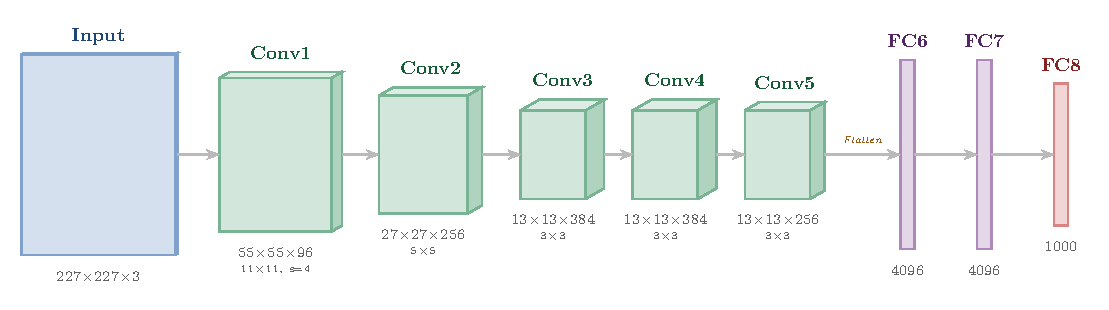
\includegraphics[width=0.95\textwidth]{images/alexnet_architecture}
    \caption[Arquitectura de AlexNet]{Arquitectura de AlexNet: red convolucional con 8 capas (5 convolucionales y 3 completamente conectadas) que alcanzó un error Top-5 del 15.3\% en ImageNet ILSVRC-2012, una mejora significativa respecto al 26.2\% del segundo mejor modelo.}
    \label{fig:alexnet}
\end{figure}

Desde la perspectiva matemática, el principio arquitectónico central de las \glspl{CNN} es la \textit{compartición de pesos} (weight sharing): los mismos kernels se aplican en todas las posiciones espaciales, lo que constituye precisamente la realización de la equivarianza traslacional como sesgo inductivo. La conectividad local de cada kernel, combinada con la composición jerárquica de capas (de bordes simples a representaciones abstractas), permite que la red construya progresivamente representaciones de complejidad creciente. Sin embargo, la restricción al grupo de traslaciones constituye también la limitación fundamental de estas arquitecturas, motivando las extensiones geométricas desarrolladas en las secciones posteriores de este capítulo.

Las convoluciones no solo se pueden aplicar en imágenes, sino que podemos extrapolarlas a cualquier dimensión. Por ejemplo, en el caso de las series temporales, podemos aplicar convoluciones en una dimensión y, en el caso de volúmenes 3D, podemos aplicar convoluciones en tres dimensiones. La formulación es similar:

\begin{equation}
    (I * K)(x) = \sum_{u=-k}^{k} I(x+u)K(u)
    \label{eq:convolution1d}
\end{equation}

\begin{equation}
    (I * K)(x,y,z) = \sum_{u=-k}^{k}\sum_{v=-k}^{k}\sum_{w=-k}^{k} I(x+u, y+v, z+w)K(u,v,w)
    \label{eq:convolution3d}
\end{equation}

\subsection{Fundamentos Matemáticos y Limitaciones de las CNNs Clásicas}\label{subsec:fundamentos_limitaciones_cnn}

\subsubsection{Convolución como Operación Equivariante}\label{subsubsec:convolucion_equivariante}

La propiedad fundamental que hace exitosas a las \glspl{CNN} es su equivarianza a traslaciones: cuando la entrada se traslada, la salida se traslada de la misma manera. Esta propiedad, que exploraremos con un ejemplo simple, es la base de su eficiencia en el procesamiento de imágenes.

\begin{example}[Equivarianza a Traslaciones en 1D]\label{ex:equivarianza_traslaciones_1d}
Considere una señal 1D $f: \mathbb{Z} \to \mathbb{R}$ y un kernel $K = [-1, 0, 1]$ (detector de bordes). 
La acción de traslación por $\tau \in \mathbb{Z}$ está dada por $(T_\tau f)(n) = f(n-\tau)$.

Sea $f = [1, 2, 1, 0, 0]$ y $\tau = 1$. Usando la definición~\eqref{eq:convolution1d} con extensión por ceros fuera del dominio:
\begin{align}
(T_1 f) &= [0, 1, 2, 1, 0] \quad \text{(señal trasladada)} \\
(f * K) &= [2, 0, -2, -1, 0] \quad \text{(convolución original)} \\
((T_1 f) * K) &= [1, 2, 0, -2, -1] \quad \text{(convolución de señal trasladada)} \\
T_1((f * K)) &= [1, 2, 0, -2, -1] \quad \text{(traslación de convolución)}
\end{align}

Observamos que $((T_1 f) * K) = T_1((f * K))$, verificando la equivarianza.
\end{example}

Esta propiedad de equivarianza es fundamental para entender tanto las fortalezas como las limitaciones de las \glspl{CNN}. Los conceptos formales de equivarianza y su generalización a otros grupos de transformaciones se desarrollan en detalle en el \autoref{ch:gdl}.

\begin{figure}[htbp]
	\centering
	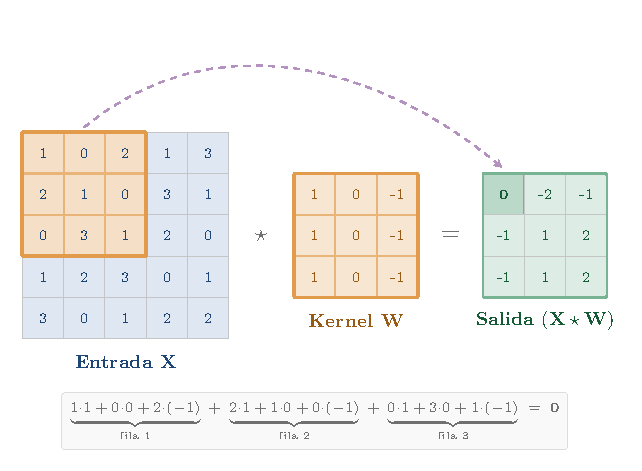
\includegraphics[width=0.85\textwidth]{images/convolution_operation}
	\caption[Operación convolucional 2D]{Operación convolucional 2D: un kernel $\mathbf{W}$ de tamaño $3 \times 3$ se desliza sobre la imagen de entrada $\mathbf{X}$, computando el producto interno local en cada posición para producir el mapa de activación de salida $(\mathbf{X} \star \mathbf{W})$.}
	\label{fig:convolution_operation}
\end{figure}

\begin{definition}[Convolución Discreta]\label{def:discrete_convolution}
Para funciones \(f, g: \mathbb{Z}^d \to \mathbb{R}\), la \textit{convolución discreta} es:
\[
(f * g)(x) = \sum_{a \in \mathbb{Z}^d} f(a)\,g(x - a)
\]
donde la suma recorre todos los puntos \(a\) del dominio \(\mathbb{Z}^d\). En la práctica, si \(f\) tiene soporte finito (como en una imagen digital), la suma se reduce a los índices donde \(f(a) \neq 0\).
\end{definition}

\begin{definition}[Convolución Continua]\label{def:continuous_convolution}
Para funciones \(f, g: \mathbb{R}^d \to \mathbb{R}\), la \textit{convolución continua} es:
\[
(f * g)(x) = \int_{\mathbb{R}^d} f(a)\,g(x - a) \, \mathrm{d}a
\]
donde la integral se toma respecto a la medida de Lebesgue sobre todo \(\mathbb{R}^d\), y existe cuando \(f, g \in L^1(\mathbb{R}^d)\) o bajo condiciones de soporte compacto.
\end{definition}

La convolución discreta puede verse como una discretización de la convolución continua, donde la integral se aproxima mediante una suma de Riemann. En el contexto de procesamiento de imágenes digitales, trabajamos con la versión discreta, mientras que en señales analógicas o análisis teórico se emplea la versión continua.

\begin{proposition}[Propiedades Algebraicas de la Convolución]\label{prop:propiedades_convolucion}
La convolución discreta satisface las siguientes propiedades para funciones
\(f, g, h: \mathbb{Z}^d \to \mathbb{R}\) con soporte finito:
\begin{enumerate}
    \item \textbf{Conmutatividad}: \(f * g = g * f\)
    \item \textbf{Asociatividad}: \((f * g) * h = f * (g * h)\)
    \item \textbf{Distributividad}: \(f * (g + h) = f * g + f * h\)
    \item \textbf{Elemento neutro}: \(f * \delta = f\), donde \(\delta\) es la delta de Kronecker
\end{enumerate}
\end{proposition}

\begin{proof}
\textbf{(1) Conmutatividad.} Mediante el cambio de variable \(b = x - a\):
\begin{align}
(f * g)(x) &= \sum_{a \in \mathbb{Z}^d} f(a)\,g(x - a) = \sum_{b \in \mathbb{Z}^d} f(x - b)\,g(b) = (g * f)(x)
\end{align}

\textbf{(2) Asociatividad.} Por aplicación directa de la definición y cambio de orden de sumación (Fubini discreto):
\begin{align}
((f * g) * h)(x) &= \sum_{b \in \mathbb{Z}^d} (f * g)(b)\,h(x - b) = \sum_{b \in \mathbb{Z}^d} \left[\sum_{a \in \mathbb{Z}^d} f(a)\,g(b - a)\right] h(x - b) \nonumber \\
                  &= \sum_{a \in \mathbb{Z}^d} f(a) \sum_{b \in \mathbb{Z}^d} g(b - a)\,h(x - b)
\end{align}
Con el cambio \(c = b - a\):
\begin{align}
&= \sum_{a \in \mathbb{Z}^d} f(a) \sum_{c \in \mathbb{Z}^d} g(c)\,h(x - a - c) = \sum_{a \in \mathbb{Z}^d} f(a)\,(g * h)(x - a) = (f * (g * h))(x)
\end{align}

\textbf{(3) Distributividad.} Por linealidad de la suma:
\begin{align}
(f * (g + h))(x) &= \sum_{a \in \mathbb{Z}^d} f(a)\,(g + h)(x - a) \nonumber \\
                  &= \sum_{a \in \mathbb{Z}^d} f(a)\,g(x - a) + \sum_{a \in \mathbb{Z}^d} f(a)\,h(x - a) = (f * g)(x) + (f * h)(x)
\end{align}

\textbf{(4) Elemento neutro.} La delta de Kronecker satisface \(\delta(a) = 1\) si \(a = 0\) y \(\delta(a) = 0\) en otro caso:
\begin{align}
(f * \delta)(x) &= \sum_{a \in \mathbb{Z}^d} f(a)\,\delta(x - a) = f(x)
\end{align}
ya que \(\delta(x - a) \neq 0\) únicamente cuando \(a = x\).
\end{proof}

\begin{theorem}[Equivarianza de la Convolución a Traslaciones]\label{theorem:convolution_translation_equivariance}
La operación de convolución es equivariante al grupo de traslaciones \(T = \mathbb{Z}^d\):
\[
T_b(f * g) = (T_b f) * g = f * (T_b g)
\]
donde \(T_b f(x) = f(x - b)\) es la traslación por \(b\).
\end{theorem}

\begin{proof}
Para la primera igualdad, mediante el cambio de índice $a' = a - b$:
\begin{align}
[(T_b f) * g](x) &= \sum_a (T_b f)(a) g(x - a) = \sum_a f(a - b) g(x - a) \\
                  &= \sum_{a'} f(a') g(x - a' - b) = (f * g)(x - b) = [T_b(f * g)](x)
\end{align}
Para la segunda igualdad:
\begin{align}
[T_b(f * g)](x) &= (f * g)(x - b) = \sum_a f(a)g((x-b) - a) \\
                 &= \sum_a f(a)g((x - a) - b) = \sum_a f(a)[T_b g](x - a) \\
                 &= [f * (T_b g)](x)
\end{align}
\end{proof}

La equivarianza a traslaciones implica que los pesos del kernel deben ser compartidos espacialmente, lo que reduce drásticamente el número de parámetros comparado con una red completamente conectada. Esta propiedad fundamental se generaliza en la \autoref{sec:group_convolutions}.

\subsubsection{Limitaciones de las CNNs Clásicas}

\begin{example}[Falta de Equivarianza Rotacional]
Considere una imagen de un dígito ``6'' y su rotación de $180^{\circ}$ que parece un ``9''. Una \gls{CNN} estándar debe aprender estas transformaciones desde los datos mediante aumentación de datos, en lugar de incorporarlas estructuralmente. Si $R_{90}$ denota una rotación de $90^{\circ}$:
\[
f(R_{90}(\text{imagen})) \neq R_{90}(f(\text{imagen}))
\]
Esto ilustra cómo las \glspl{CNN} estándar solo son equivariantes a traslaciones, no a otras transformaciones geométricas.
\end{example}

Aunque las \glspl{CNN} han revolucionado la visión por computador, su diseño presenta limitaciones fundamentales que restringen su aplicabilidad. Estas limitaciones, que surgen directamente de su restricción a la equivarianza de traslaciones, pueden clasificarse en cuatro categorías principales:

\begin{enumerate}
    \item \textbf{Limitaciones de simetría}: Solo son equivariantes a traslaciones discretas $\mathbb{Z}^d$, requiriendo aumentación de datos para transformaciones como rotaciones, reflexiones o escalamientos. Esto es ineficiente tanto computacional como estadísticamente.
    
    \item \textbf{Limitaciones topológicas}: Diseñadas para grillas regulares euclidianas, son inadecuadas para datos con topologías no triviales como grafos, nubes de puntos, variedades riemannianas o complejos simpliciales.
    
    \item \textbf{Limitaciones de localidad}: Su dependencia de estructuras locales implica que las relaciones globales requieren múltiples capas para ser capturadas, limitando eficiencia en dominios donde las dependencias de largo alcance son críticas.
    
    \item \textbf{Limitaciones de campo receptivo}: El crecimiento lineal del campo receptivo con la profundidad requiere arquitecturas profundas para capturar patrones globales, introduciendo problemas de gradiente desaparecido e ineficiencia computacional.
\end{enumerate}

Estas limitaciones sistemáticas han motivado el desarrollo de extensiones geométricas que constituyen el núcleo del presente capítulo. Cada extensión aborda conjuntos específicos de estas limitaciones mediante la generalización controlada de las simetrías preservadas:

\begin{itemize}
    \item \textbf{Convoluciones de Grupo} (\autoref{sec:group_convolutions}): Generalizan equivarianza desde traslaciones hacia grupos finitos como $D_4$ (rotaciones y reflexiones), abordando las limitaciones de simetría.
    \item \textbf{Spherical/Steerable \glspl{CNN}}: Extienden equivarianza a grupos continuos como $SO(2)$ y $SO(3)$, permitiendo procesamiento de datos esféricos y tridimensionales.
    \item \textbf{\glspl{CNN} en Variedades} (\autoref{sec:manifold_cnns}): Superan las limitaciones topológicas mediante la generalización a superficies curvas y variedades riemannianas.
    \item \textbf{Convoluciones Gauge} (\autoref{sec:gauge_cnns}): Introducen equivarianza a transformaciones gauge en fibrados, la generalización más abstracta posible.
\end{itemize}

Esta progresión sistemática desde la equivarianza restringida hacia la generalidad completa constituye la narrativa central del capítulo y ejemplifica los principios del \gls{GDL} en acción.

\section{Análisis Armónico y Convoluciones Espectrales}\label{sec:analisis_armonico}

Mientras que las extensiones geométricas de \glspl{CNN} abordan las limitaciones de simetría, topología y localidad mediante la generalización directa de las operaciones convolucionales, el análisis armónico proporciona una perspectiva dual y complementaria que revela la estructura matemática profunda subyacente a todas estas arquitecturas. Esta sección desarrolla el marco teórico que conecta las convoluciones clásicas con sus generalizaciones espectrales, desde los fundamentos del análisis de Fourier hasta las aplicaciones modernas en dominios irregulares.

La dualidad espacial-espectral constituye uno de los principios más fundamentales en matemáticas aplicadas: mientras que las operaciones de convolución se realizan naturalmente en el dominio espacial, su estructura algebraica se comprende mejor en el dominio frecuencial. El teorema de convolución, $\mathcal{F}[f * g] = \mathcal{F}[f] \cdot \mathcal{F}[g]$, revela que la operación convolucional compleja en el espacio se reduce a una simple multiplicación puntual en frecuencia. Esta perspectiva no solo proporciona ventajas computacionales mediante algoritmos como la \gls{FFT}, sino que también ofrece perspectivas profundas sobre qué características aprenden las redes neuronales y cómo pueden diseñarse arquitecturas más eficientes.

En el contexto del \gls{GDL}, el análisis armónico adquiere una importancia fundamental al proporcionar las herramientas matemáticas necesarias para generalizar las convoluciones a dominios no euclidianos. La teoría de representaciones de grupos, desarrollada en el marco del análisis armónico, permite diseñar capas convolucionales que preservan automáticamente las simetrías específicas del dominio de datos. Del mismo modo, el análisis espectral en grafos mediante el Laplaciano proporciona la base teórica para las \glspl{GCN} espectrales, mientras que las wavelets ofrecen representaciones jerárquicas naturales que se alinean con las arquitecturas profundas modernas.

\subsection{Fundamentos del Análisis de Fourier}\label{subsec:fundamentos_fourier}

El análisis de Fourier constituye una de las herramientas matemáticas más poderosas para el estudio de fenómenos periódicos y el análisis frecuencial. Su aplicación en el contexto de redes neuronales convolucionales permite una comprensión profunda de las propiedades espectrales de los filtros y operaciones convolucionales.

\begin{definition}[Transformada de Fourier Continua]\label{def:transformada_fourier_continua}
Sea $f: \mathbb{R}^d \to \mathbb{C}$ una función integrable. La \textit{transformada de Fourier} de $f$ se define como:
\begin{equation}
\mathcal{F}[f](\omega) = \hat{f}(\omega) = \int_{\mathbb{R}^d} f(x) e^{-2\pi i \omega \cdot x} dx
\end{equation}
donde $\omega \in \mathbb{R}^d$ representa la variable frecuencial y $\omega \cdot x = \sum_{j=1}^d \omega_j x_j$ es el producto escalar euclidiano.
\end{definition}

\textbf{Condiciones de Existencia.} La transformada de Fourier está bien definida para funciones en $L^1(\mathbb{R}^d)$ (funciones absolutamente integrables). Para funciones en $L^2(\mathbb{R}^d)$, la transformada se define como límite en media cuadrática.

\begin{definition}[Transformada de Fourier Inversa]\label{def:transformada_fourier_inversa}
Si $\hat{f} \in L^1(\mathbb{R}^d)$, la \textit{transformada de Fourier inversa} se define como:
\begin{equation}
\mathcal{F}^{-1}[\hat{f}](x) = f(x) = \int_{\mathbb{R}^d} \hat{f}(\omega) e^{2\pi i \omega \cdot x} d\omega
\end{equation}
\end{definition}

\begin{theorem}[Teorema de Inversión de Fourier]\label{thm:inversion_fourier}
Si $f, \hat{f} \in L^1(\mathbb{R}^d)$, entonces:
\begin{equation}
f(x) = \mathcal{F}^{-1}[\mathcal{F}[f]](x) = \int_{\mathbb{R}^d} \hat{f}(\omega) e^{2\pi i \omega \cdot x} d\omega
\end{equation}
para casi todo $x \in \mathbb{R}^d$. Para la demostración, véase \citep[Theorem~8.26]{Folland1999}.
\end{theorem}

\begin{definition}[Convolución en $\mathbb{R}^d$]\label{def:convolucion_continua}
Para funciones $f, g: \mathbb{R}^d \to \mathbb{C}$, la \textit{convolución} se define como:
\begin{equation}
(f * g)(x) = \int_{\mathbb{R}^d} f(y) g(x - y) dy = \int_{\mathbb{R}^d} f(x - y) g(y) dy
\end{equation}
cuando la integral converge.
\end{definition}

\subsubsection{Ejemplos Concretos de Transformadas de Fourier}

Los siguientes ejemplos ilustran las propiedades fundamentales de la transformada de Fourier en contextos relevantes para el análisis de CNNs.

\begin{example}[Transformada de la Función Gaussiana]\label{ex:fourier_gaussian}
Para la función gaussiana $f(x) = e^{-\alpha x^2}$ con $\alpha > 0$:
\begin{equation}
\mathcal{F}[e^{-\alpha x^2}](\omega) = \sqrt{\frac{\pi}{\alpha}} e^{-\pi^2 \omega^2/\alpha}
\end{equation}

\textbf{Propiedades notables}:
\begin{itemize}
    \item La transformada de una gaussiana es otra gaussiana
    \item Localización dual: función estrecha $\Leftrightarrow$ transformada ancha
    \item Minimiza el principio de incertidumbre tiempo-frecuencia
    \item Fundamental en filtros de suavizado para CNNs
\end{itemize}
\end{example}

\begin{example}[Transformada de la Función Escalón]\label{ex:fourier_step}
Para la función escalón unitaria $\mathbf{1}_{[0,1]}(x)$:
\begin{equation}
\mathcal{F}[\mathbf{1}_{[0,1]}](\omega) = \frac{e^{-2\pi i \omega} - 1}{-2\pi i \omega} = \frac{\sin(\pi\omega)}{\pi\omega} e^{-\pi i \omega}
\end{equation}

\textbf{Interpretación para CNNs}:
\begin{itemize}
    \item Representa filtros de promediado (kernels constantes)
    \item La función sinc en frecuencia indica comportamiento pasa-bajos
    \item Oscilaciones en frecuencia debidas a discontinuidades en el dominio espacial
\end{itemize}
\end{example}

\begin{example}[Transformada de la Función Sinc]\label{ex:fourier_sinc}
Para la función sinc $f(x) = \frac{\sin(\pi x)}{\pi x}$:
\begin{equation}
\mathcal{F}[\operatorname{sinc}(x)](\omega) = \mathbf{1}_{[-1/2,1/2]}(\omega)
\end{equation}

Esta dualidad escalón $\leftrightarrow$ sinc es fundamental:
\begin{itemize}
    \item Filtro ideal pasa-bajos en frecuencia $\rightarrow$ respuesta sinc en espacio
    \item Imposible de implementar exactamente (soporte infinito)
    \item Inspira diseño de filtros aproximados en CNNs espectrales
\end{itemize}
\end{example}

\begin{example}[Transformada del Delta de Dirac]\label{ex:fourier_delta}
Para la distribución delta $\delta(x)$:
\begin{equation}
\mathcal{F}[\delta](\omega) = 1 \quad \text{y} \quad \mathcal{F}[1](\omega) = \delta(\omega)
\end{equation}

\textbf{Significado para CNNs}:
\begin{itemize}
    \item Delta espacial = espectro plano (todas las frecuencias presentes)
    \item Constante espacial = impulso frecuencial (frecuencia cero únicamente)
    \item Principio de localización en el análisis espectral de filtros
\end{itemize}
\end{example}

\textbf{Implementación Computacional.} En la práctica, estas transformadas se calculan mediante \gls{FFT} discreta. El análisis espectral de kernels comunes revela patrones importantes:

\textbf{Proceso de análisis}:
\begin{enumerate}
    \item \textbf{Padding}: Se extiende el kernel con ceros para mejorar la resolución frecuencial
    \item \textbf{\gls{FFT} 2D}: Se calcula la transformada rápida de Fourier bidimensional
    \item \textbf{Centrado del espectro}: Se aplica fftshift para centrar las frecuencias bajas
    \item \textbf{Análisis de magnitud y fase}: Se separan los componentes para interpretación
\end{enumerate}

\textbf{Ejemplos de kernels típicos}:
\begin{itemize}
    \item \textbf{Sobel X}: Detector de bordes con respuesta pasa-altos en dirección horizontal
    \item \textbf{Gaussiano}: Filtro pasa-bajos con respuesta suave y simétrica
    \item \textbf{Laplaciano}: Detector de bordes isotrópico con respuesta pasa-altos
\end{itemize}

\textbf{Conexión con Wavelets.} Las transformadas anteriores motivan el uso de wavelets en CNNs:
\begin{itemize}
    \item \textbf{Gaussianas}: Base para wavelets Gabor (análisis tiempo-frecuencia)
    \item \textbf{Escalones}: Relacionados con wavelets de Haar (características de borde)
    \item \textbf{Sinc}: Fundamento de wavelets Daubechies (reconstrucción perfecta)
\end{itemize}
La capacidad de analizar múltiples escalas simultáneamente hace que las wavelets sean especialmente atractivas para arquitecturas CNN jerárquicas.

\begin{figure}[htbp]
	\centering
	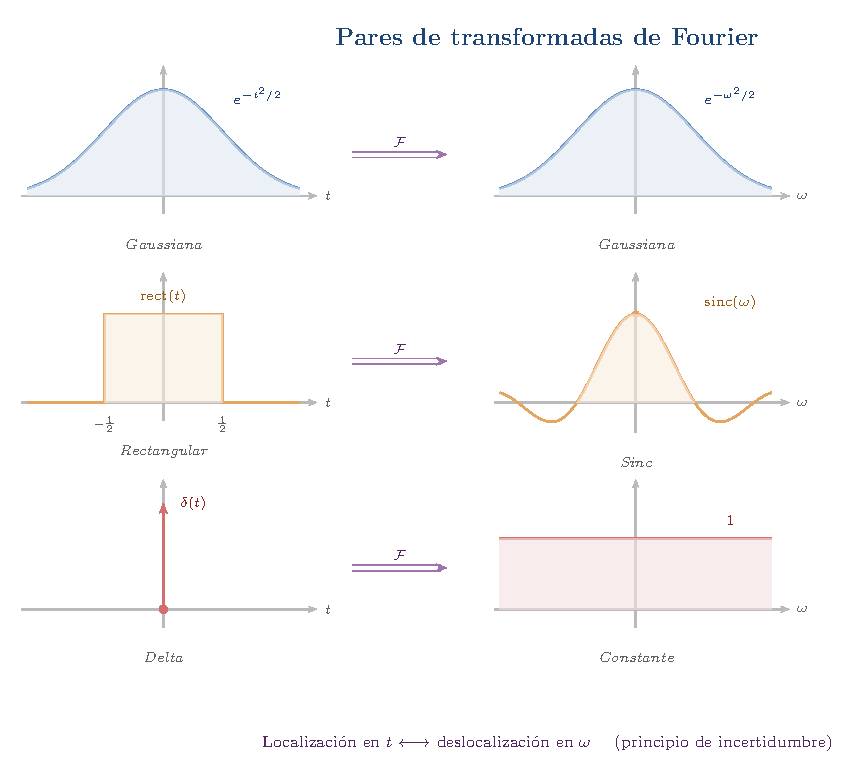
\includegraphics[width=0.85\textwidth]{images/fourier_pairs}
	\caption[Pares de transformadas de Fourier]{Pares de transformadas de Fourier: correspondencia entre señales en el dominio temporal ($t$) y sus representaciones en el dominio frecuencial ($\omega$). Se observa la dualidad localización-deslocalización que fundamenta el principio de incertidumbre.}
	\label{fig:fourier_pairs}
\end{figure}

\subsection{Propiedades Fundamentales del Análisis Armónico}\label{subsec:propiedades_fundamentales}

\begin{theorem}[Teorema de Convolución en Dominio de Fourier]\label{thm:convolucion_fourier}
Para funciones \(f, g: \mathbb{R}^d \to \mathbb{C}\):
\[
\mathcal{F}[f * g] = \mathcal{F}[f] \cdot \mathcal{F}[g]
\]
donde \(\mathcal{F}\) denota la transformada de Fourier.
\end{theorem}

\begin{proof}
Sean $f, g \in L^1(\mathbb{R}^d)$. Aplicando el teorema de Fubini:
\begin{align}
\mathcal{F}[f * g](\omega) &= \int_{\mathbb{R}^d} (f * g)(x) e^{-2\pi i\omega \cdot x} dx \\
&= \int_{\mathbb{R}^d} \left[\int_{\mathbb{R}^d} f(y)g(x-y) \, dy\right] e^{-2\pi i\omega \cdot x} dx \\
&= \int_{\mathbb{R}^d} f(y) \left[\int_{\mathbb{R}^d} g(x-y) e^{-2\pi i\omega \cdot x} dx\right] dy \\
&= \int_{\mathbb{R}^d} f(y) e^{-2\pi i\omega \cdot y} \mathcal{F}[g](\omega) \, dy \\
&= \mathcal{F}[f](\omega) \cdot \mathcal{F}[g](\omega)
\end{align}
donde en el cuarto paso se usa el cambio de variable $z = x - y$ y la definición de $\mathcal{F}[g]$.
\end{proof}

\begin{corollary}[Eficiencia Computacional vía FFT]
La convolución puede computarse en \(O(n \log n)\) usando:
\[
f * g = \mathcal{F}^{-1}[\mathcal{F}[f] \cdot \mathcal{F}[g]]
\]
\end{corollary}

\begin{proof}
Por el teorema de convolución anterior, $\mathcal{F}[f * g] = \mathcal{F}[f] \cdot \mathcal{F}[g]$, luego $f * g = \mathcal{F}^{-1}[\mathcal{F}[f] \cdot \mathcal{F}[g]]$. Para señales discretas de longitud $n$, la \gls{FFT} computa $\mathcal{F}[f]$ y $\mathcal{F}[g]$ cada una en $O(n \log n)$ operaciones, la multiplicación puntual $\mathcal{F}[f] \cdot \mathcal{F}[g]$ requiere $O(n)$ operaciones, y la transformada inversa $\mathcal{F}^{-1}$ tiene el mismo coste $O(n \log n)$. El coste total es $O(n \log n)$, frente al $O(n^2)$ del cálculo directo de la convolución.
\end{proof}

\begin{theorem}[Identidad de Plancherel]\label{thm:plancherel}
Para funciones $f, g \in L^2(\mathbb{R}^d)$, la transformada de Fourier preserva el producto interno:
\begin{equation}
\langle f, g \rangle_{L^2} = \langle \hat{f}, \hat{g} \rangle_{L^2}
\end{equation}
En particular, $\|\hat{f}\|_{L^2} = \|f\|_{L^2}$ (isometría). Véase \citep[Theorem~8.29]{Folland1999}.
\end{theorem}

\textbf{Importancia en Redes Neuronales.} La identidad de Plancherel garantiza que las operaciones en el dominio frecuencial preservan la energía de las señales, lo cual es fundamental para la estabilidad numérica de algoritmos espectrales en CNNs.

\begin{definition}[Transformada de Fourier Discreta (DFT)]\label{def:dft}
Para una secuencia finita $\{x_n\}_{n=0}^{N-1}$, la \textbf{transformada de Fourier discreta} se define como:
\begin{equation}
X_k = \sum_{n=0}^{N-1} x_n e^{-2\pi i kn/N}, \quad k = 0, 1, \ldots, N-1
\end{equation}
\end{definition}

\begin{definition}[Fast Fourier Transform (FFT)]\label{def:fft}
El algoritmo \gls{FFT} calcula la DFT en tiempo $O(N \log N)$ en lugar de $O(N^2)$ mediante factorización recursiva:
\begin{equation}
X_k = \sum_{n=0}^{N/2-1} x_{2n} e^{-2\pi i kn/(N/2)} + e^{-2\pi i k/N} \sum_{n=0}^{N/2-1} x_{2n+1} e^{-2\pi i kn/(N/2)}
\end{equation}
\end{definition}

\begin{theorem}[Teorema de Muestreo de Nyquist-Shannon]\label{thm:nyquist_shannon}
Sea $f: \mathbb{R} \to \mathbb{C}$ una función de banda limitada con $\hat{f}(\omega) = 0$ para $|\omega| > W$. Entonces $f$ está completamente determinada por sus muestras en intervalos de $1/(2W)$:
\begin{equation}
f(t) = \sum_{n=-\infty}^{\infty} f\left(\frac{n}{2W}\right) \operatorname{sinc}(2W(t - \frac{n}{2W}))
\end{equation}
donde $\operatorname{sinc}(x) = \sin(\pi x)/(\pi x)$. Este resultado fundamental fue establecido por \citet{Shannon1948}.
\end{theorem}

\textbf{Frecuencia de Nyquist y Aliasing.} La frecuencia de Nyquist $f_N = W$ es la máxima frecuencia que puede representarse sin aliasing. En CNNs, el sub-muestreo (pooling) puede introducir aliasing si no se aplican filtros anti-aliasing apropiados.

\begin{definition}[Serie de Fourier]\label{def:serie_fourier}
Para una función periódica $f: \mathbb{R} \to \mathbb{C}$ con período $T$, la serie de Fourier se expresa como:
\begin{equation}
f(t) = \sum_{n=-\infty}^{\infty} c_n e^{2\pi i n t/T}
\end{equation}
donde los coeficientes son $c_n = \frac{1}{T} \int_0^T f(t) e^{-2\pi i n t/T} dt$.
\end{definition}

\begin{definition}[Transformada de Fourier Ventaneada (STFT)]\label{def:stft}
Para analizar señales no estacionarias, se define:
\begin{equation}
\text{STFT}_f(t, \omega) = \int_{-\infty}^{\infty} f(\tau) w(\tau - t) e^{-2\pi i \omega \tau} d\tau
\end{equation}
donde $w$ es una función ventana (típicamente Gaussiana o Hann).
\end{definition}

\textbf{Principio de Incertidumbre Tiempo-Frecuencia.} La STFT está sujeta al principio de incertidumbre: $\Delta t \cdot \Delta \omega \geq \frac{1}{4\pi}$, lo que implica un trade-off fundamental entre resolución temporal y frecuencial.

\subsubsection{Ejemplos Numéricos del Teorema de Convolución}

El teorema de convolución es fundamental para entender la eficiencia computacional de las CNNs espectrales. Los siguientes ejemplos ilustran su aplicación práctica.

\begin{example}[Convolución Rápida vía FFT: Análisis de Complejidad]\label{ex:convolution_fft_complexity}
Considere la convolución de una imagen $f \in \mathbb{R}^{N \times N}$ con un kernel $g \in \mathbb{R}^{K \times K}$.

\textbf{Método directo}:
\begin{equation}
(f * g)[i,j] = \sum_{u=0}^{K-1} \sum_{v=0}^{K-1} f[i-u, j-v] \cdot g[u,v]
\end{equation}
Complejidad: $O(N^2 K^2)$

\textbf{Método espectral}:
\begin{align}
\hat{f} &= \text{FFT2D}(f) \quad \text{[Complejidad: } O(N^2 \log N)\text{]} \\
\hat{g} &= \text{FFT2D}(\text{pad}(g, N)) \quad \text{[Complejidad: } O(N^2 \log N)\text{]} \\
\hat{h} &= \hat{f} \odot \hat{g} \quad \text{[Complejidad: } O(N^2)\text{]} \\
h &= \text{IFFT2D}(\hat{h}) \quad \text{[Complejidad: } O(N^2 \log N)\text{]}
\end{align}
Complejidad total: $O(N^2 \log N)$

\textbf{Punto de equilibrio}: El método espectral es más eficiente cuando $K > O(\log N)$.
\end{example}

\begin{example}[Implementación Práctica: Convolución Rápida]\label{ex:fast_convolution_implementation}
La convolución rápida mediante \gls{FFT} sigue estos pasos algorítmicos:

\textbf{Algoritmo de convolución espectral}:
\begin{enumerate}
    \item \textbf{Dimensionamiento}: Calcular tamaño óptimo como potencia de 2 para eficiencia de \gls{FFT}
    \item \textbf{Transformación}: Aplicar FFT2D tanto a la imagen como al kernel con padding apropiado
    \item \textbf{Multiplicación}: Producto elemento a elemento en el dominio frecuencial
    \item \textbf{Inversión}: IFFT2D para recuperar el resultado en dominio espacial
    \item \textbf{Recorte}: Extraer la región válida del resultado
\end{enumerate}

\textbf{Análisis comparativo de rendimiento}:
Para diferentes tamaños de imagen y kernel, los resultados típicos muestran:
\begin{itemize}
    \item \textbf{Imágenes pequeñas (64$\times$64)}: Método directo más eficiente para kernels $< 7 \times 7$
    \item \textbf{Imágenes medianas (256$\times$256)}: \gls{FFT} ventajosa para kernels $> 5 \times 5$
    \item \textbf{Imágenes grandes (512$\times$512)}: \gls{FFT} consistentemente más rápida con speedups de 2-10x
    \item \textbf{Error numérico}: Típicamente $< 10^{-12}$ con precisión doble
\end{itemize}
\end{example}

\begin{example}[Análisis de Error Numérico]\label{ex:numerical_error_analysis}
El análisis de errores en convoluciones \gls{FFT} revela patrones importantes de estabilidad numérica:

\textbf{Metodología de análisis}:
\begin{enumerate}
    \item \textbf{Señales de prueba}: Utilizar matrices aleatorias con distribución normal
    \item \textbf{Kernel de referencia}: Laplaciano discreto como caso de prueba estándar
    \item \textbf{Comparación}: Convolución directa vs. método \gls{FFT}
    \item \textbf{Métricas}: Error relativo en norma L2
\end{enumerate}

\textbf{Resultados empíricos observados}:
\begin{itemize}
    \item \textbf{Error relativo típico}: $10^{-12}$ a $10^{-14}$ con precisión doble
    \item \textbf{Escalabilidad}: El error crece logarítmicamente con el tamaño de imagen
    \item \textbf{Estabilidad de kernel}: Kernels bien condicionados minimizan propagación
    \item \textbf{Accumulation pattern}: Errores se concentran en componentes de alta frecuencia
\end{itemize}

\textbf{Implicaciones prácticas}:
La alta precisión numérica (error $< 10^{-12}$) hace que el método \gls{FFT} sea prácticamente equivalente al método directo para la mayoría de aplicaciones de deep learning, donde la precisión single ($\sim 10^{-7}$) es estándar.
\end{example}

\textbf{Optimizaciones Avanzadas.} En implementaciones prácticas de CNNs espectrales:

\textbf{1. Uso de FFTW (Fastest Fourier Transform in the West)}:
\begin{itemize}
    \item Optimización específica para hardware (SIMD, multi-core)
    \item Planning automático del algoritmo \gls{FFT} óptimo
    \item Speedups de 2-5x sobre implementaciones básicas
\end{itemize}

\textbf{2. Overlap-Add/Overlap-Save}:
Para convoluciones con kernels grandes en CNNs, se usan técnicas de procesamiento por bloques:
\begin{itemize}
    \item Dividir la imagen en bloques superpuestos
    \item FFT de bloques pequeños (más eficiente en cache)
    \item Reconstrucción con manejo de solapamiento
\end{itemize}

\textbf{3. GPU Acceleration}:
\begin{itemize}
    \item cuFFT para implementaciones en CUDA
    \item Uso de memoria compartida para minimizar transferencias
    \item Batching de múltiples convoluciones simultáneas
\end{itemize}

\subsection{Análisis Armónico en Grupos}\label{subsec:analisis_armonico_grupos}

El análisis armónico en grupos generaliza la transformada de Fourier clásica a espacios más generales con estructura de grupo, proporcionando las herramientas matemáticas fundamentales para las convoluciones geométricas en redes neuronales.

Recordamos que la \textit{medida de Haar} de un grupo localmente compacto $G$ es la única medida de Borel (salvo constante) invariante por traslaciones izquierdas: $\mu(gE) = \mu(E)$ para todo $g \in G$ (\autoref{def:medida_haar_gdl} del \autoref{ch:gdl}).\label{def:medida_haar}

\textbf{Existencia y Unicidad.} El teorema de Haar garantiza que toda medida de Haar existe y es única salvo constante multiplicativa. Para grupos finitos, la medida de Haar es la medida de conteo.

Los conceptos fundamentales de representaciones de grupos (incluyendo la definición de representación (\autoref{def:representacion_grupo}), representaciones irreducibles (\autoref{def:representacion_irreducible}) y el teorema de Peter-Weyl (\autoref{thm:peter_weyl})) se desarrollan en el \autoref{ch:gdl}, Sección~\ref{subsec:teoria_grupos_representaciones}. Aquí recordamos brevemente las herramientas específicas del análisis armónico que utilizaremos para CNNs.

El \textit{carácter} de una representación $\rho: G \to GL(\mathbb{C}^d)$ es la función $\chi(g) = \operatorname{tr}(\rho(g))$, y los caracteres irreducibles satisfacen la relación de ortogonalidad $\frac{1}{|G|} \sum_{g \in G} \chi_i(g) \overline{\chi_j(g)} = \delta_{ij}$. A partir de estas herramientas se define la transformada de Fourier en grupos finitos: para $f: G \to \mathbb{C}$ y representación irreducible $\rho_i$ de dimensión $d_i$,
\begin{equation}\label{eq:fourier_grupo_finito}
\hat{f}(\rho_i) = \sum_{g\in G} f(g)\rho_i(g) \in \mathbb{C}^{d_i \times d_i},
\end{equation}
con inversión $f(g) = \frac{1}{|G|} \sum_i d_i \operatorname{tr}(\hat{f}(\rho_i) \rho_i(g^{-1}))$. El resultado fundamental para CNNs es el \textbf{teorema de convolución}: la transformada de Fourier convierte la convolución en grupo en producto matricial,
\begin{equation}\label{eq:convolucion_fourier_grupos}
\widehat{f *_G h}(\rho_i) = \hat{f}(\rho_i) \hat{h}(\rho_i),
\end{equation}
generalizando el resultado clásico de la DFT.

\begin{example}[Grupo Cíclico $\mathbb{Z}_n$]\label{ex:grupo_ciclico_fourier}
Para el grupo cíclico de orden $n$, las representaciones irreducibles son unidimensionales:
\begin{equation}
\rho_k(j) = e^{-2\pi i jk/n}, \quad k = 0, 1, \ldots, n-1
\end{equation}
La transformada de Fourier se reduce a la DFT clásica:
\begin{equation}
\hat{f}(k) = \sum_{j=0}^{n-1} f(j) e^{-2\pi i jk/n}
\end{equation}
\end{example}

\begin{example}[Grupo Diédrico $D_n$]\label{ex:grupo_diedrico_fourier}
Para el grupo diédrico de orden $2n$ (simetrías de un $n$-gono), las representaciones incluyen:
\begin{itemize}
    \item \textbf{Representaciones triviales}: $\rho(g) = 1$ para todo $g$
    \item \textbf{Representaciones de signo}: $\rho(r^j) = 1$, $\rho(sr^j) = -1$
    \item \textbf{Representaciones bidimensionales}: Para rotaciones y reflexiones
\end{itemize}
\end{example}

\subsubsection{Ejemplos Detallados de Análisis Armónico en Grupos Finitos}

Los siguientes ejemplos proporcionan cálculos explícitos que ilustran la construcción práctica de representaciones y transformadas de Fourier para grupos relevantes en GDL.

\begin{example}[Grupo Cíclico $\mathbb{Z}_4$: Cálculos Explícitos]\label{ex:grupo_z4_detallado}
El grupo cíclico $\mathbb{Z}_4 = \{0, 1, 2, 3\}$ con operación suma módulo 4 representa rotaciones de $90^\circ$.

\textbf{Representaciones irreducibles}:
Las representaciones 1D son homomorfismos $\rho_k: \mathbb{Z}_4 \to \mathbb{C}^*$:
\begin{align}
\rho_0(j) &= 1 \quad \text{(representación trivial)} \\
\rho_1(j) &= i^j \quad \text{donde } i = e^{2\pi i/4} \\
\rho_2(j) &= (-1)^j \\
\rho_3(j) &= (-i)^j
\end{align}

\textbf{Matriz de caracteres}:
\begin{equation}
\chi = \begin{bmatrix}
1 & 1 & 1 & 1 \\
1 & i & -1 & -i \\
1 & -1 & 1 & -1 \\
1 & -i & -1 & i
\end{bmatrix}
\end{equation}

\textbf{Transformada de Fourier discreta}:
Para una función $f: \mathbb{Z}_4 \to \mathbb{C}$, $f = (f_0, f_1, f_2, f_3)^T$:
\begin{equation}
\hat{f} = \chi f = \begin{bmatrix}
f_0 + f_1 + f_2 + f_3 \\
f_0 + if_1 - f_2 - if_3 \\
f_0 - f_1 + f_2 - f_3 \\
f_0 - if_1 - f_2 + if_3
\end{bmatrix}
\end{equation}

\textbf{Aplicación en G-CNNs}:
\begin{itemize}
    \item Cada representación $\rho_k$ corresponde a un canal en convoluciones equivariantes a rotaciones de $90^\circ$
    \item Los filtros se expresan como combinaciones lineales de las representaciones
    \item La equivarianza se preserva automáticamente por la estructura del grupo
\end{itemize}
\end{example}

\begin{example}[Grupo Diédrico $D_3$: Simetrías del Triángulo]\label{ex:grupo_d3_detallado}
$D_3$ contiene las 6 simetrías del triángulo equilátero: 3 rotaciones y 3 reflexiones.

\textbf{Elementos del grupo}:
\begin{itemize}
    \item $e$: identidad
    \item $r, r^2$: rotaciones de $120^\circ, 240^\circ$
    \item $s, sr, sr^2$: reflexiones respecto a las mediatrices
\end{itemize}

\textbf{Representaciones irreducibles}:
\begin{enumerate}
    \item \textbf{Trivial} $\rho^{(1)}$: $\rho^{(1)}(g) = 1$ para todo $g$
    \item \textbf{Alternante} $\rho^{(2)}$: 
    \begin{align}
    \rho^{(2)}(r^k) &= 1, \quad k = 0,1,2 \\
    \rho^{(2)}(sr^k) &= -1, \quad k = 0,1,2
    \end{align}
    \item \textbf{Estándar bidimensional} $\rho^{(3)}$:
    \begin{align}
    \rho^{(3)}(e) &= \begin{bmatrix} 1 & 0 \\ 0 & 1 \end{bmatrix} \\
    \rho^{(3)}(r) &= \begin{bmatrix} -1/2 & -\sqrt{3}/2 \\ \sqrt{3}/2 & -1/2 \end{bmatrix} \\
    \rho^{(3)}(r^2) &= \begin{bmatrix} -1/2 & \sqrt{3}/2 \\ -\sqrt{3}/2 & -1/2 \end{bmatrix} \\
    \rho^{(3)}(s) &= \begin{bmatrix} 1 & 0 \\ 0 & -1 \end{bmatrix}
    \end{align}
\end{enumerate}

\textbf{Tabla de caracteres}:
\begin{equation}
\begin{array}{c|ccc}
 & e & r, r^2 & s, sr, sr^2 \\
\hline
\rho^{(1)} & 1 & 1 & 1 \\
\rho^{(2)} & 1 & 1 & -1 \\
\rho^{(3)} & 2 & -1 & 0
\end{array}
\end{equation}

\textbf{Implementación computacional}:
La implementación práctica del grupo diédrico $D_3$ requiere:

\textbf{Representaciones matriciales}:
\begin{itemize}
    \item \textbf{Identidad}: Matriz identidad $2 \times 2$
    \item \textbf{Rotaciones}: Matrices de rotación para $120^\circ$ y $240^\circ$
    \item \textbf{Reflexiones}: Combinación de reflexión básica con rotaciones
\end{itemize}

\textbf{Transformada de Fourier en $D_3$}:
Para una función $f: D_3 \to \mathbb{C}$, el proceso computacional implica:
\begin{enumerate}
    \item \textbf{Proyección trivial}: Promedio de todos los valores de función
    \item \textbf{Proyección alternante}: Diferencia entre rotaciones y reflexiones
    \item \textbf{Proyección bidimensional}: Combinación lineal más compleja
\end{enumerate}

\textbf{Ejemplo de análisis}:
Para la función característica de rotaciones $f(g) = 1$ si $g$ es rotación, $f(g) = 0$ si es reflexión:
\begin{itemize}
    \item Componente trivial: $\frac{3}{6} = 0.5$
    \item Componente alternante: $\frac{3-0}{6} = 0.5$
    \item Componente 2D: Vector con estructura específica
\end{itemize}
\end{example}

\textbf{Conexión con G-CNNs Prácticas.} Los cálculos anteriores se traducen directamente en arquitecturas de redes neuronales:

\textbf{Para $\mathbb{Z}_4$-CNNs}:
\begin{itemize}
    \item 4 orientaciones de filtros $(0^\circ, 90^\circ, 180^\circ, 270^\circ)$
    \item Cada canal de salida corresponde a una representación irreducible
    \item La convolución se implementa como suma sobre órbitas del grupo
\end{itemize}

\textbf{Para $D_3$-CNNs}:
\begin{itemize}
    \item 6 transformaciones de filtros (3 rotaciones $\times$ 2 reflexiones)
    \item Manejo especial de la representación 2D (canales acoplados)
    \item Aplicación en análisis de simetrías triangulares (cristalografía, materiales)
\end{itemize}

\textbf{Implementación eficiente}:
La transformada de Fourier rápida en grupos finitos se implementa mediante:
\begin{equation}
\text{Complejidad}: O(|G|^{3/2}) \text{ vs } O(|G|^2) \text{ para DFT directa}
\end{equation}

\begin{example}[Conexión con Wavelets en Grupos]\label{ex:wavelets_grupos_finitos}
Los grupos finitos también admiten análisis wavelet mediante funciones madre apropiadas.

\textbf{Wavelet madre en $\mathbb{Z}_4$}:
\begin{equation}
\psi(j) = \delta_{j,1} - \delta_{j,3} \quad \text{(función diferencia)}
\end{equation}

\textbf{Familia wavelet}:
\begin{equation}
\psi_{k,j}(m) = \psi((m - j) \bmod 4) \cdot \omega_4^{km}
\end{equation}
donde $\omega_4 = e^{2\pi i/4}$.

Esta construcción permite análisis multiresolución en espacios discretos con simetría rotacional.
\end{example}

\begin{definition}[Transformada de Fourier en Grupos Compactos]\label{def:fourier_grupos_compactos}
Para un grupo compacto $G$ y función $f \in L^2(G)$, la transformada de Fourier se define mediante el teorema de Peter-Weyl:
\begin{equation}
f = \sum_{\lambda \in \widehat{G}} d_\lambda \operatorname{tr}(\hat{f}(\lambda) U^\lambda)
\end{equation}
donde $\widehat{G}$ indexa las representaciones irreducibles.
\end{definition}

\subsubsection{Análisis Armónico en SO(2) y SO(3)}

\begin{definition}[Armónicos Circulares en SO(2)]\label{def:armonicos_circulares}
Para el grupo de rotaciones planares $SO(2) \cong S^1$, las representaciones irreducibles son:
\begin{equation}
U^n(\theta) = e^{in\theta}, \quad n \in \mathbb{Z}
\end{equation}
Una función $f: S^1 \to \mathbb{C}$ se expande como:
\begin{equation}
f(\theta) = \sum_{n=-\infty}^{\infty} c_n e^{in\theta}
\end{equation}
\end{definition}

\begin{definition}[Armónicos Esféricos en SO(3)]\label{def:armonicos_esfericos}
Para el grupo de rotaciones tridimensionales $SO(3)$, las funciones sobre la esfera $S^2$ se expanden en armónicos esféricos:
\begin{equation}
f(\theta, \phi) = \sum_{l=0}^{\infty} \sum_{m=-l}^{l} c_{lm} Y_l^m(\theta, \phi)
\end{equation}
donde $Y_l^m$ son los armónicos esféricos de grado $l$ y orden $m$.
\end{definition}

\textbf{Aplicaciones del Teorema de Peter-Weyl.} El teorema de Peter-Weyl (\autoref{thm:peter_weyl}, \autoref{ch:gdl}) proporciona la base teórica para:
\begin{itemize}
    \item La descomposición en canales en G-CNNs
    \item El diseño de filtros equivariantes en esferas
    \item La parametrización eficiente de convoluciones en grupos de Lie
\end{itemize}

\subsection{Análisis Espectral en Grafos}\label{subsec:analisis_espectral_grafos}

El análisis espectral en grafos extiende las ideas del análisis de Fourier a dominios irregulares, proporcionando las bases matemáticas para convoluciones espectrales en redes neuronales sobre grafos. Los fundamentos teóricos del Laplaciano de grafo, incluyendo definiciones y propiedades espectrales, se desarrollan en el \autoref{ch:gdl}, Sección~\ref{subsec:geometria_topologica_grafos}. Para la matriz Laplaciana $L = D - A$ y sus variantes normalizadas, véase la \autoref{def:laplaciano_grafo} y la \autoref{prop:propiedades_espectrales_laplaciano_grafos}.

En esta sección nos enfocamos en las aplicaciones del análisis espectral al diseño de convoluciones en grafos, asumiendo familiaridad con el Laplaciano $L$ y su versión normalizada $\mathcal{L} = D^{-1/2} L D^{-1/2}$.

\begin{theorem}[Teorema Espectral para el Laplaciano]\label{thm:espectral_laplaciano}
Sea $L$ la matriz Laplaciana de un grafo conectado. Entonces:
\begin{enumerate}
    \item Los eigenvalores satisfacen $0 = \lambda_0 < \lambda_1 \leq \lambda_2 \leq \cdots \leq \lambda_{n-1}$
    \item El eigenvector asociado a $\lambda_0 = 0$ es $\phi_0 = \frac{1}{\sqrt{n}} \mathbf{1}$
    \item Los eigenvectores $\{\phi_k\}_{k=0}^{n-1}$ forman una base ortonormal de $\mathbb{R}^n$
    \item La multiplicidad de $\lambda_0$ es igual al número de componentes conexas
\end{enumerate}
Para la demostración, véase \citep[Capítulos~1--2]{Chung1997} y la \autoref{prop:propiedades_espectrales_laplaciano_grafos}.
\end{theorem}

La transformada de Fourier en grafos (\autoref{def:transformada_fourier_grafos}, \autoref{ch:gdl}) proyecta señales sobre los eigenvectores del Laplaciano: $\hat{f}(\lambda_k) = \langle \mathbf{f}, \phi_k \rangle$, con forma matricial $\hat{f} = U^T f$. A partir de esta transformada se definen las convoluciones espectrales:

\begin{definition}[Convolución Espectral en Grafos]\label{def:convolucion_espectral_grafos}
Para una función $f: V \to \mathbb{R}$ y un filtro espectral $g: \mathbb{R}_+ \to \mathbb{R}$:
\begin{equation}
(g \star f)(v_i) = \sum_{k=0}^{n-1} g(\lambda_k) \hat{f}(\lambda_k) \phi_k(v_i)
\end{equation}
En forma matricial: $g \star f = \Phi g(\Lambda) \Phi^T f$, donde $\Phi = [\phi_0, \ldots, \phi_{n-1}]$ y $\Lambda = \operatorname{diag}(\lambda_0, \ldots, \lambda_{n-1})$.
\end{definition}

\begin{theorem}[Interpretación Frecuencial]\label{thm:interpretacion_frecuencial_grafos}
Los eigenvalores del Laplaciano tienen interpretación frecuencial:
\begin{itemize}
    \item \textbf{Frecuencias bajas} ($\lambda_k$ pequeño): Eigenvectores varían suavemente sobre el grafo
    \item \textbf{Frecuencias altas} ($\lambda_k$ grande): Eigenvectores oscilan rápidamente entre vértices adyacentes
    \item \textbf{Filtros pasa-bajos}: $g(\lambda) \approx 1$ para $\lambda$ pequeño, $g(\lambda) \approx 0$ para $\lambda$ grande
\end{itemize}
\end{theorem}

\begin{proof}
La interpretación se justifica mediante el cociente de Rayleigh. Para una señal $\mathbf{f} \in \mathbb{R}^n$ sobre el grafo, la variación total se mide como:
\[
\mathbf{f}^T L \mathbf{f} = \sum_{(i,j) \in E} w_{ij}(f_i - f_j)^2
\]
El $k$-ésimo eigenvector $\phi_k$ minimiza esta variación total sujeto a ortogonalidad con los eigenvectores previos: $\lambda_k = \min_{\mathbf{f} \perp \phi_0, \ldots, \phi_{k-1}} \frac{\mathbf{f}^T L \mathbf{f}}{\mathbf{f}^T \mathbf{f}}$. Luego eigenvectores con eigenvalores pequeños minimizan la variación entre nodos adyacentes (variación suave, baja frecuencia), mientras que eigenvalores grandes corresponden a eigenvectores con alta variación (oscilaciones rápidas, alta frecuencia).
\end{proof}

\begin{figure}[htbp]
    \centering
    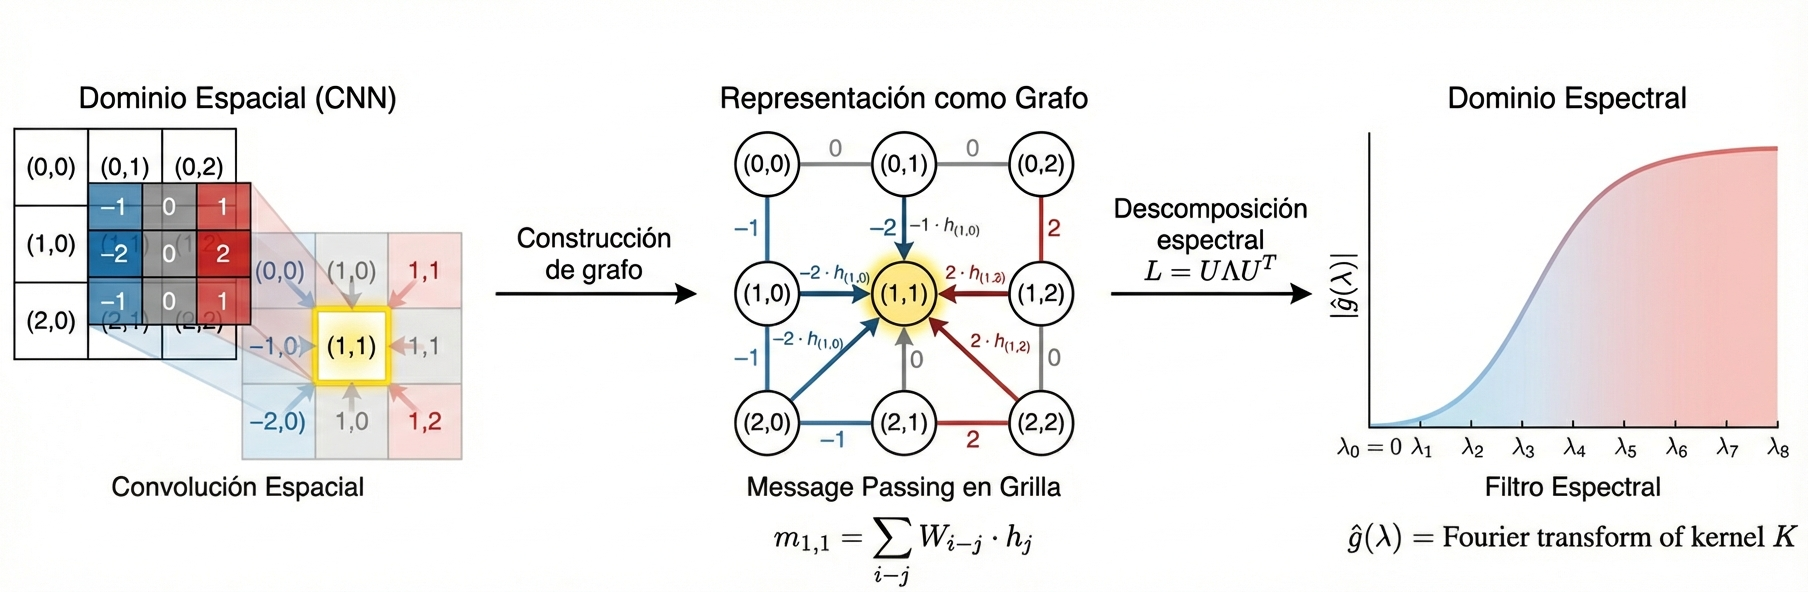
\includegraphics[width=0.85\textwidth]{images/cnn_graph_kernel_spectral}
    \caption[De kernel CNN a representación espectral en grafos]{Transformación de un kernel de CNN a representación espectral en grafos. El kernel espacial de una CNN tradicional (izquierda) se puede interpretar como un filtro espectral sobre el grafo de la grilla regular (derecha), donde los autovalores del Laplaciano determinan las frecuencias y el filtro modula cada componente frecuencial.}
    \label{fig:cnn_graph_kernel_spectral}
\end{figure}

\begin{theorem}[Localización Espectral]\label{thm:localizacion_espectral}
Si un filtro espectral $g(\lambda)$ satisface las condiciones de decaimiento:
\begin{equation}
|g^{(k)}(\lambda)| \leq C_k (1 + \lambda)^{-k-\epsilon}
\end{equation}
para algún $\epsilon > 0$ y constantes $C_k$, donde $g^{(k)}$ denota la $k$-ésima derivada, entonces $g$ produce operaciones localmente soportadas en el grafo.
\end{theorem}

\begin{proof}[Esbozo de demostración]
El kernel del filtro en el dominio del grafo es $K(i,j) = \sum_k g(\lambda_k) \phi_k(i) \phi_k(j)$, donde $\{\lambda_k, \phi_k\}$ son los pares propios del Laplaciano. La condición de decaimiento sobre $g^{(k)}$ implica, mediante integración por partes generalizada, que el kernel $K(i,j)$ decae exponencialmente con la distancia geodésica $d(i,j)$ en el grafo. Formalmente, para nodos $i,j$ a distancia $d(i,j) > K$ se tiene $|K(i,j)| \leq C \cdot \alpha^{d(i,j)}$ para algún $\alpha < 1$, lo que garantiza que la operación de filtrado es esencialmente local. Véase \citep[Theorem~5.5]{hammond2011wavelets} para la demostración completa en el contexto de wavelets en grafos.
\end{proof}

\subsubsection{Aproximación Polinomial de Filtros}

Para hacer las convoluciones espectrales computacionalmente eficientes, se aproximan los filtros mediante polinomios, evitando la diagonalización explícita del Laplaciano.

\begin{definition}[Filtros Polinomiales]\label{def:filtros_polinomiales}
Un filtro espectral $g(\lambda)$ se aproxima como:
\begin{equation}
g(\lambda) \approx \sum_{k=0}^K \theta_k p_k(\lambda)
\end{equation}
donde $\{p_k\}$ es una base polinomial y $\{\theta_k\}$ son parámetros entrenables.
\end{definition}

\begin{example}[Aproximación de Chebyshev]\label{ex:chebyshev_aproximacion}
Usando polinomios de Chebyshev $T_k$ en el intervalo $[-1, 1]$:
\begin{equation}
g(\tilde{\lambda}) = \sum_{k=0}^K \theta_k T_k(\tilde{\lambda})
\end{equation}
donde $\tilde{\lambda} = 2\lambda/\lambda_{\max} - 1$ reescala los eigenvalues.
\end{example}

\begin{theorem}[Eficiencia Computacional]\label{thm:eficiencia_chebyshev}
La aproximación de Chebyshev permite calcular $g(L)f$ en tiempo $O(K|E|)$ sin diagonalizar $L$, usando la recurrencia:
\begin{align}
\bar{x}_0 &= f \\
\bar{x}_1 &= \tilde{L} f \\
\bar{x}_k &= 2\tilde{L}\bar{x}_{k-1} - \bar{x}_{k-2}, \quad k \geq 2
\end{align}
donde $\tilde{L} = 2L/\lambda_{\max} - I$.
\end{theorem}

\begin{proof}
Por la recurrencia de Chebyshev, $T_k(\tilde{L})f$ se calcula inductivamente: $\bar{x}_0 = f$ requiere $O(n)$, $\bar{x}_1 = \tilde{L}f$ requiere una multiplicación matriz-vector dispersa con coste $O(|E|)$ (pues $\tilde{L}$ tiene a lo sumo $2|E| + n$ entradas no nulas), y cada paso $\bar{x}_k = 2\tilde{L}\bar{x}_{k-1} - \bar{x}_{k-2}$ requiere igualmente $O(|E|)$. Como se realizan $K$ pasos de recurrencia, el coste total es $O(K|E|)$. Nótese que no se requiere calcular los eigenvalores ni eigenvectores de $L$, pues la recurrencia opera directamente con la matriz dispersa $\tilde{L}$.
\end{proof}

\subsubsection{Ejemplo Completo: Análisis Espectral de un Grafo Pequeño}

El siguiente ejemplo ilustra todos los conceptos anteriores mediante cálculos explícitos en un grafo de 4 nodos.

\begin{example}[Laplaciano de Grafo Triangular con Vértice Aislado]\label{ex:laplaciano_triangulo_4_nodos}
Considere el grafo $G$ con 4 vértices y aristas $E = \{(1,2), (1,3), (2,3), (3,4)\}$:

\begin{center}
\begin{tikzpicture}[scale=1.2]
    \node[circle, draw, fill=gdlblue!20] (1) at (0, 1) {1};
    \node[circle, draw, fill=gdlblue!20] (2) at (-1, -0.5) {2};
    \node[circle, draw, fill=gdlblue!20] (3) at (1, -0.5) {3};
    \node[circle, draw, fill=gdlgreen!20] (4) at (2.5, 0) {4};
    
    \draw[thick] (1) -- (2);
    \draw[thick] (1) -- (3);
    \draw[thick] (2) -- (3);
    \draw[thick] (3) -- (4);
\end{tikzpicture}
\end{center}

\textbf{1. Matriz de adyacencia}:
\begin{equation}
A = \begin{bmatrix}
0 & 1 & 1 & 0 \\
1 & 0 & 1 & 0 \\
1 & 1 & 0 & 1 \\
0 & 0 & 1 & 0
\end{bmatrix}
\end{equation}

\textbf{2. Matriz de grados}:
\begin{equation}
D = \begin{bmatrix}
2 & 0 & 0 & 0 \\
0 & 2 & 0 & 0 \\
0 & 0 & 3 & 0 \\
0 & 0 & 0 & 1
\end{bmatrix}
\end{equation}

\textbf{3. Laplaciano no normalizado}:
\begin{equation}
L = D - A = \begin{bmatrix}
2 & -1 & -1 & 0 \\
-1 & 2 & -1 & 0 \\
-1 & -1 & 3 & -1 \\
0 & 0 & -1 & 1
\end{bmatrix}
\end{equation}

\textbf{4. Cálculo de eigenvalores y eigenvectores}:
El polinomio característico es:
\begin{equation}
\det(L - \lambda I) = \lambda(\lambda - 1)(\lambda - 3)(\lambda - 4)
\end{equation}

Los eigenvalores son: $\lambda_0 = 0, \lambda_1 = 1, \lambda_2 = 3, \lambda_3 = 4$.

\textbf{Eigenvectores (calculados y normalizados)}:
\begin{align}
\phi_0 &= \tfrac{1}{2}(1, 1, 1, 1)^T \quad \text{(vector constante, $\lambda_0 = 0$)} \\
\phi_1 &= \tfrac{1}{\sqrt{6}}(-1, -1, 0, 2)^T \quad \text{(variación suave, $\lambda_1 = 1$)} \\
\phi_2 &= \tfrac{1}{\sqrt{2}}(1, -1, 0, 0)^T \quad \text{(contraste 1-2, $\lambda_2 = 3$)} \\
\phi_3 &= \tfrac{1}{2\sqrt{3}}(1, 1, -3, 1)^T \quad \text{(alta frecuencia, $\lambda_3 = 4$)}
\end{align}

Se verifica que $L\phi_k = \lambda_k \phi_k$, $\|\phi_k\| = 1$ y $\langle \phi_i, \phi_j \rangle = \delta_{ij}$ para todo $i, j$.

\textbf{5. Interpretación frecuencial}:
\begin{itemize}
    \item $\phi_0$ (DC): función constante sobre todo el grafo
    \item $\phi_1$ (baja frecuencia): variación suave, vértice 4 contrasta con vértices 1-2
    \item $\phi_2$ (media frecuencia): contraste entre vértices 1 y 2
    \item $\phi_3$ (alta frecuencia): oscilación rápida, vértice 3 contrasta fuertemente con sus vecinos
\end{itemize}

\textbf{6. Convolución espectral - Ejemplo práctico}:
Sea $f = (1, 0, -1, 2)^T$ una señal en el grafo y $g(\lambda) = e^{-\lambda/2}$ un filtro pasa-bajos.

\textbf{Transformada de Fourier de $f$}:
\begin{align}
\hat{f}_0 &= \phi_0^T f = \tfrac{1}{2}(1 + 0 - 1 + 2) = 1 \\
\hat{f}_1 &= \phi_1^T f = \tfrac{1}{\sqrt{6}}(-1 + 0 + 0 + 4) = \tfrac{3}{\sqrt{6}} = \tfrac{\sqrt{6}}{2} \\
\hat{f}_2 &= \phi_2^T f = \tfrac{1}{\sqrt{2}}(1 - 0 + 0 + 0) = \tfrac{1}{\sqrt{2}} = \tfrac{\sqrt{2}}{2} \\
\hat{f}_3 &= \phi_3^T f = \tfrac{1}{2\sqrt{3}}(1 + 0 + 3 + 2) = \tfrac{6}{2\sqrt{3}} = \sqrt{3}
\end{align}

\textbf{Aplicación del filtro}:
\begin{align}
g(\lambda_0) \hat{f}_0 &= e^{0} \cdot 1 = 1 \\
g(\lambda_1) \hat{f}_1 &= e^{-1/2} \cdot \tfrac{\sqrt{6}}{2} \approx 0.74 \\
g(\lambda_2) \hat{f}_2 &= e^{-3/2} \cdot \tfrac{\sqrt{2}}{2} \approx 0.16 \\
g(\lambda_3) \hat{f}_3 &= e^{-2} \cdot \sqrt{3} \approx 0.23
\end{align}

\textbf{Señal filtrada}:
\begin{equation}
f_{\text{filtered}} = \sum_{k=0}^{3} g(\lambda_k)\hat{f}_k \phi_k \approx (0.38, 0.15, 0.30, 1.17)^T
\end{equation}

\textbf{Interpretación}: El filtro pasa-bajos ha suavizado la señal, reduciendo especialmente las componentes de alta frecuencia ($\lambda_2 = 3$ y $\lambda_3 = 4$) mientras preserva la componente constante.
\end{example}

\textbf{Implementación Computacional del Ejemplo.} La verificación computacional del ejemplo sigue esta metodología:

\textbf{Construcción del grafo}:
\begin{enumerate}
    \item Definir 4 nodos con conectividad específica: $(1,2)$, $(1,3)$, $(2,3)$, $(3,4)$
    \item Calcular matrices de adyacencia y Laplaciano usando bibliotecas estándar
    \item Verificar propiedades básicas: simetría, semi-definitud positiva
\end{enumerate}

\textbf{Análisis espectral}:
\begin{itemize}
    \item \textbf{Eigenvalores}: $\{0, 1, 3, 4\}$ con interpretación frecuencial clara
    \item \textbf{Eigenvectores}: Base ortogonal para representar señales en el grafo
    \item \textbf{Verificación}: Comprobar ortogonalidad y propiedades de normalization
\end{itemize}

\textbf{Convolución espectral}:
Para la señal de prueba $f = [1, 0, -1, 2]^T$ y filtro pasa-bajos $g(\lambda) = e^{-\lambda/2}$:
\begin{enumerate}
    \item \textbf{Transformada directa}: $\hat{f} = U^T f$ usando eigenvectores
    \item \textbf{Filtrado}: Multiplicación por $g(\lambda_k)$ para cada componente
    \item \textbf{Transformada inversa}: $f_{filtrado} = U \hat{f}_{filtrado}$
\end{enumerate}

\textbf{Resultados numéricos}:
El filtro pasa-bajos produce una señal suavizada $\approx [0.38, 0.15, 0.30, 1.17]^T$, demostrando la atenuación de componentes de alta frecuencia mientras preserva las tendencias globales.

\textbf{Observaciones del Ejemplo.} Este ejemplo ilustra conceptos clave del análisis espectral en grafos:

\textbf{1. Conectividad y multiplicidad}:
El grafo es conexo, por lo que $\lambda_0 = 0$ tiene multiplicidad 1.

\textbf{2. Interpretación geométrica}:
- Los eigenvectores de baja frecuencia capturan la estructura global
- Los de alta frecuencia revelan variaciones locales entre nodos adyacentes

\textbf{3. Filtrado eficaz}:
El filtro pasa-bajos $e^{-\lambda/2}$ preserva la componente DC y atenúa progresivamente las frecuencias más altas.

\textbf{4. Complejidad computacional}:
- Diagonalización: $O(n^3)$ para $n = 4$ (trivial)
- En grafos grandes, se prefiere la aproximación polinomial Chebyshev

\begin{example}[Otros Tipos de Filtros Espectrales]\label{ex:otros_filtros_espectrales}
\leavevmode
\begin{enumerate}
    \item \textbf{Filtros Racionales}: $g(\lambda) = \frac{P(\lambda)}{Q(\lambda)}$ donde $P, Q$ son polinomios
    \item \textbf{Filtros de Lanczos}: $g(\lambda) = \theta \cdot \operatorname{sinc}(\pi\lambda/\lambda_{\max})$
    \item \textbf{Splines}: Funciones spline por tramos sobre el espectro
    \item \textbf{Filtros Wavelets}: Basados en wavelets espectrales en grafos
\end{enumerate}
\end{example}

\textbf{Trade-off Localización vs Eficiencia.} Existe un trade-off fundamental:
\begin{itemize}
    \item \textbf{Filtros espectrales globales}: Más expresivos pero $O(n^3)$ para diagonalización
    \item \textbf{Aproximaciones polinomiales}: Locales y eficientes $O(K|E|)$ pero menos expresivos
    \item \textbf{Grado del polinomio $K$}: Controla el radio de localización espacial
\end{itemize}

\subsection{Bases Wavelets y Análisis Multiresolución}\label{subsec:wavelets_multirresolucion}

Las wavelets proporcionan una alternativa a la transformada de Fourier que permite análisis tiempo-frecuencia simultáneo, superando las limitaciones del principio de incertidumbre. Su aplicación en redes neuronales ofrece representaciones jerárquicas naturales.

\begin{definition}[Wavelet Madre]\label{def:wavelet_madre}
Una función $\psi \in L^2(\mathbb{R})$ es una \textbf{wavelet madre} si satisface la condición de admisibilidad:
\begin{equation}
C_\psi = \int_{-\infty}^{\infty} \frac{|\hat{\psi}(\omega)|^2}{|\omega|} d\omega < \infty
\end{equation}
donde $\hat{\psi}$ es la transformada de Fourier de $\psi$.
\end{definition}

\textbf{Implicaciones de la Condición de Admisibilidad.} La condición $C_\psi < \infty$ implica que $\hat{\psi}(0) = 0$, lo que significa $\int_{-\infty}^{\infty} \psi(t) dt = 0$. Esto garantiza que las wavelets tienen media cero y proporcionan análisis local.

\begin{definition}[Transformada Wavelet Continua]\label{def:transformada_wavelet_continua}
Para una función $f \in L^2(\mathbb{R})$ y wavelet madre $\psi$, la transformada wavelet continua se define como:
\begin{equation}
W_f(a, b) = \frac{1}{\sqrt{|a|}} \int_{-\infty}^{\infty} f(t) \psi^*\left(\frac{t-b}{a}\right) dt
\end{equation}
donde $a \in \mathbb{R}\setminus\{0\}$ es el parámetro de escala y $b \in \mathbb{R}$ es el parámetro de traslación.
\end{definition}

\begin{theorem}[Fórmula de Reconstrucción Wavelet]\label{thm:reconstruccion_wavelet}
Si $\psi$ satisface la condición de admisibilidad, entonces:
\begin{equation}
f(t) = \frac{1}{C_\psi} \int_{-\infty}^{\infty} \int_{-\infty}^{\infty} W_f(a, b) \psi_{a,b}(t) \frac{da \, db}{a^2}
\end{equation}
donde $\psi_{a,b}(t) = \frac{1}{\sqrt{|a|}} \psi\left(\frac{t-b}{a}\right)$.

Véase la Sección~\ref{sec:reconstruccion_wavelet} del \autoref{ch:teoremas_complementarios} para la demostración completa.
\end{theorem}

\begin{definition}[Análisis Multiresolución (MRA)]\label{def:mra}
Un \textbf{análisis multiresolución} de $L^2(\mathbb{R})$ es una secuencia de subespacios cerrados $\{V_j\}_{j \in \mathbb{Z}}$ que satisface:
\begin{enumerate}
    \item \textbf{Inclusión}: $\cdots \subset V_{-1} \subset V_0 \subset V_1 \subset \cdots$
    \item \textbf{Densidad}: $\overline{\bigcup_{j \in \mathbb{Z}} V_j} = L^2(\mathbb{R})$
    \item \textbf{Separación}: $\bigcap_{j \in \mathbb{Z}} V_j = \{0\}$
    \item \textbf{Escalado}: $f(x) \in V_j \Leftrightarrow f(2x) \in V_{j+1}$
    \item \textbf{Traslación}: $f(x) \in V_0 \Rightarrow f(x-k) \in V_0$ para $k \in \mathbb{Z}$
    \item \textbf{Base de Riesz}: Existe $\phi \in V_0$ tal que $\{\phi(x-k)\}_{k \in \mathbb{Z}}$ es base de Riesz de $V_0$
\end{enumerate}
\end{definition}

\begin{definition}[Función de Escala]\label{def:funcion_escala}
La función $\phi$ en la condición 6 del MRA se llama \textbf{función de escala} o \textbf{wavelet padre}. Satisface la ecuación de escalado:
\begin{equation}
\phi(x) = \sqrt{2} \sum_{k \in \mathbb{Z}} h_k \phi(2x - k)
\end{equation}
donde $\{h_k\}$ son los coeficientes de escalado.
\end{definition}

\begin{definition}[Wavelet Ortogonal]\label{def:wavelet_ortogonal}
Dado un MRA con función de escala $\phi$, la \textbf{wavelet ortogonal} asociada se define como:
\begin{equation}
\psi(x) = \sqrt{2} \sum_{k \in \mathbb{Z}} g_k \phi(2x - k)
\end{equation}
donde $g_k = (-1)^k h_{1-k}$ están relacionados con los coeficientes de escalado.
\end{definition}

\begin{theorem}[Descomposición Wavelet]\label{thm:descomposicion_wavelet}
Toda función $f \in L^2(\mathbb{R})$ puede descomponerse como:
\begin{equation}
f(x) = \sum_{k \in \mathbb{Z}} c_{J,k} \phi_{J,k}(x) + \sum_{j=J}^{\infty} \sum_{k \in \mathbb{Z}} d_{j,k} \psi_{j,k}(x)
\end{equation}
donde $\phi_{j,k}(x) = 2^{j/2} \phi(2^j x - k)$ y $\psi_{j,k}(x) = 2^{j/2} \psi(2^j x - k)$.

Véase la Sección~\ref{sec:descomposicion_wavelet} del \autoref{ch:teoremas_complementarios} para la demostración.
\end{theorem}

\begin{example}[Wavelets de Haar]\label{ex:wavelets_haar}
Las wavelets de Haar son las más simples:
\begin{align}
\phi(x) &= \begin{cases} 1 & \text{si } 0 \leq x < 1 \\ 0 & \text{en otro caso} \end{cases} \\
\psi(x) &= \begin{cases} 1 & \text{si } 0 \leq x < 1/2 \\ -1 & \text{si } 1/2 \leq x < 1 \\ 0 & \text{en otro caso} \end{cases}
\end{align}
\end{example}

\begin{example}[Wavelets de Daubechies]\label{ex:wavelets_daubechies}
Las wavelets de Daubechies $D_N$ tienen soporte compacto $[0, 2N-1]$ y $N$ momentos nulos:
\begin{equation}
\int_{-\infty}^{\infty} x^k \psi(x) dx = 0, \quad k = 0, 1, \ldots, N-1
\end{equation}
\end{example}

\subsubsection{Wavelets en Grafos}

\begin{definition}[Wavelets Espectrales en Grafos]\label{def:wavelets_grafos}
Para un grafo con Laplaciano $L$ y eigenvectores $\{\phi_k\}$, las wavelets espectrales se definen como:
\begin{equation}
\psi_{s,i} = \sum_{k=0}^{n-1} g(s\lambda_k) \phi_k(i) \phi_k
\end{equation}
donde $g$ es una función wavelet madre y $s$ es el parámetro de escala.
\end{definition}

\begin{example}[GraphWavelets]\label{ex:graph_wavelets}
Una elección común para la función madre es:
\begin{equation}
g(x) = x e^{-x}
\end{equation}
que proporciona localización tanto espectral como espacial en el grafo.
\end{example}

\textbf{Ventajas de Wavelets en CNNs.} Las wavelets ofrecen ventajas específicas para redes neuronales:
\begin{itemize}
    \item \textbf{Análisis multiresolución}: Natural para arquitecturas jerárquicas
    \item \textbf{Localización}: Mejor que Fourier para características locales
    \item \textbf{Parsimonia}: Representaciones sparse para señales naturales
    \item \textbf{Invarianza por traslación}: Aproximada según el tipo de wavelet
\end{itemize}

\subsubsection{Wavelet de Morlet y Análisis Tiempo-Frecuencia}

\begin{definition}[Wavelet de Morlet]\label{def:wavelet_morlet}
La \textit{wavelet de Morlet} es una onda modulada por una gaussiana:
\begin{equation}
\psi_{\omega_0}(t) = c_\sigma \pi^{-1/4} e^{i\omega_0 t} e^{-t^2/2}
\end{equation}
donde $\omega_0 \geq 5$ es la frecuencia central y $c_\sigma$ es una constante de normalización. Su transformada de Fourier es $\hat{\psi}_{\omega_0}(\omega) = c_\sigma \pi^{-1/4} e^{-(\omega - \omega_0)^2/2}$, una gaussiana centrada en $\omega_0$.
\end{definition}

\begin{remark}[Resolución Tiempo-Frecuencia Óptima]
La wavelet de Morlet alcanza la igualdad en el principio de incertidumbre de Heisenberg-Gabor:
\[
\Delta t \cdot \Delta \omega = \frac{1}{2}
\]
lo que la convierte en la wavelet con mejor resolución simultánea en tiempo y frecuencia. A escala $a$, la wavelet $\psi_{a,b}(t) = a^{-1/2}\psi((t-b)/a)$ tiene resolución temporal $\Delta t \propto a$ y frecuencial $\Delta \omega \propto 1/a$, implementando exactamente la propiedad de multiresolución adaptativa.
\end{remark}

\subsubsection{Scattering Transform: CNNs con Wavelets Predefinidas}

La conexión más profunda entre wavelets y CNNs se establece a través del \textit{Scattering Transform} de Mallat~\citep{Mallat2012scattering}, que muestra que las primeras capas de una CNN pueden entenderse como un banco de filtros wavelet con no linealidad de módulo.

\begin{definition}[Scattering Transform]\label{def:scattering_transform}
Sea $\psi$ una wavelet madre y $\phi$ una función de escala (paso-bajo). El \textit{operador de scattering} de orden $m$ se define recursivamente:
\begin{align}
S_0 f &= f \star \phi_J \\
S_1 f &= \{|f \star \psi_{j_1}| \star \phi_J\}_{j_1} \\
S_m f &= \{|\cdots|f \star \psi_{j_1}| \star \psi_{j_2}| \cdots \star \psi_{j_m}| \star \phi_J\}_{j_1 < j_2 < \cdots < j_m}
\end{align}
donde $\psi_j(t) = 2^{-j}\psi(2^{-j}t)$ son las wavelets dilatadas y $\phi_J$ es la función de escala a la resolución más gruesa.
\end{definition}

\begin{proposition}[Propiedades del Scattering Transform]\label{prop:propiedades_scattering}
El operador de scattering $Sf = (S_0 f, S_1 f, S_2 f, \ldots)$ satisface:
\begin{enumerate}
    \item \textbf{Invarianza por traslación}: $S[\tau_c f] = S[f]$ para toda traslación $\tau_c f(t) = f(t - c)$.
    \item \textbf{Estabilidad Lipschitz a deformaciones}: Para todo difeomorfismo $\tau$ cercano a la identidad:
    \begin{equation}
    \|Sf - S(f \circ \tau)\| \leq C\|\nabla \tau\|_\infty \|f\|
    \end{equation}
    \item \textbf{Conservación de energía}: $\sum_{m=0}^{\infty} \|S_m f\|^2 = \|f\|^2$.
\end{enumerate}
\end{proposition}

\begin{proof}
(1) La traslación conmuta con la convolución: $\tau_c f \star \psi_j = \tau_c(f \star \psi_j)$. El módulo preserva esta traslación: $|\tau_c(f \star \psi_j)| = \tau_c|f \star \psi_j|$. Finalmente, la convolución con $\phi_J$ (paso-bajo a escala $2^J$) promedia sobre traslaciones menores que $2^J$, eliminando la dependencia en $c$.

(2) Dado que $\psi_j$ tiene soporte frecuencial concentrado en $|\omega| \sim 2^j$, la convolución $f \star \psi_j$ es sensible a variaciones de $f$ a escala $2^{-j}$. Una deformación $\tau$ con $\|\nabla \tau\|_\infty \leq \epsilon$ desplaza las frecuencias como máximo en $\epsilon \cdot 2^j$, que es pequeño comparado con el ancho de banda $2^j$ del filtro, produciendo un error proporcional a $\epsilon$.

(3) Se sigue de la identidad de Parseval para wavelets: $\|f\|^2 = \|f \star \phi_J\|^2 + \sum_j \|f \star \psi_j\|^2$. Aplicando iterativamente a los coeficientes $|f \star \psi_j|$ y usando que el módulo preserva la norma $L^2$, se obtiene la conservación de energía total.
\end{proof}

\begin{remark}[Scattering como CNN con Pesos Fijos]
La arquitectura del scattering transform es isomorfa a una CNN con las siguientes correspondencias:
\begin{itemize}
    \item \textbf{Filtros}: Wavelets $\psi_j$ predefinidas (no aprendidas) $\leftrightarrow$ kernels convolucionales
    \item \textbf{No linealidad}: Módulo $|{\cdot}|$ $\leftrightarrow$ ReLU
    \item \textbf{Pooling}: Convolución con $\phi_J$ $\leftrightarrow$ average pooling
    \item \textbf{Profundidad}: Orden $m$ del scattering $\leftrightarrow$ número de capas
\end{itemize}
La diferencia clave es que el scattering transform tiene garantías teóricas de estabilidad e invarianza, mientras que las CNNs entrenadas las aprenden implícitamente.
\end{remark}

\begin{figure}[htbp]
	\centering
	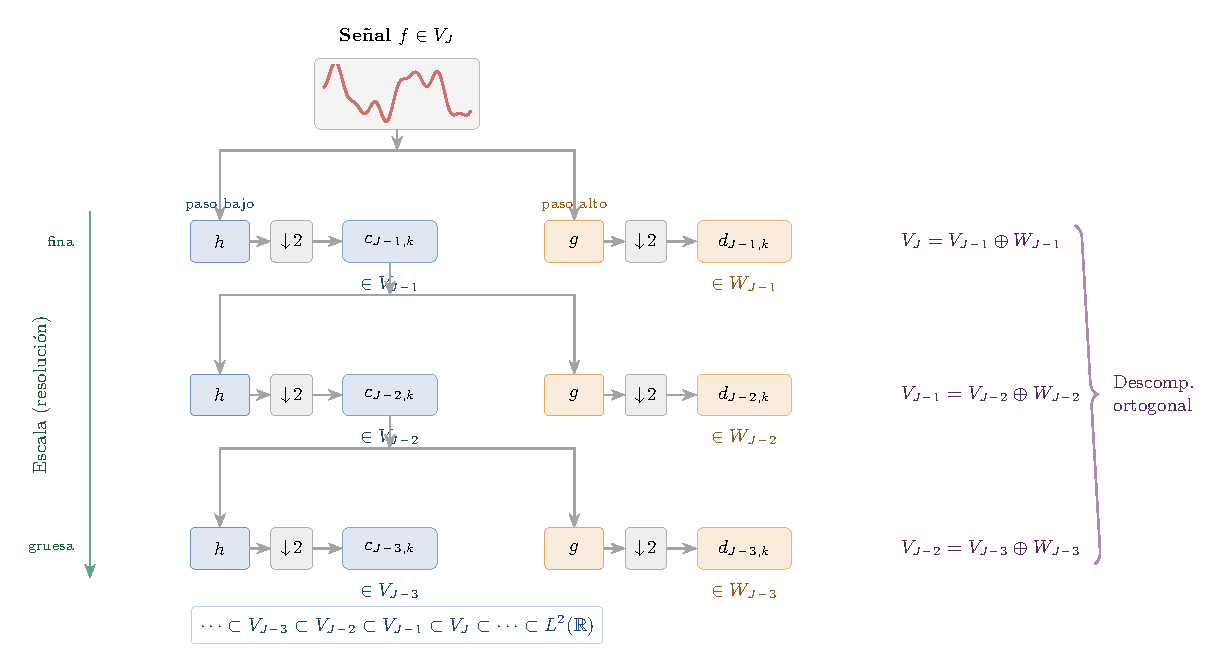
\includegraphics[width=0.85\textwidth]{images/wavelet_multiresolution}
	\caption[Descomposición wavelet multiresolución]{Descomposición wavelet multiresolución: una señal se descompone iterativamente mediante filtros paso-bajo ($h$) y paso-alto ($g$) seguidos de submuestreo ($\downarrow 2$), separando las componentes de aproximación ($c_{j,k}$) y detalle ($d_{j,k}$) a múltiples escalas.}
	\label{fig:wavelet_multiresolution}
\end{figure}

\subsection{Convoluciones Espectrales en CNNs}\label{subsec:convoluciones_espectrales_cnns}

Las convoluciones espectrales en CNNs aprovechan las propiedades del dominio frecuencial para implementar operaciones convolucionales de manera eficiente, especialmente para kernels grandes o en aplicaciones con estructura geométrica específica.

\begin{definition}[Filtro Espectral Parametrizado]\label{def:filtro_espectral_parametrizado}
Un \textbf{filtro espectral parametrizado} es una función $h_\theta: \mathbb{R}_+ \to \mathbb{R}$ donde $\theta \in \mathbb{R}^p$ son parámetros entrenables. El filtro actúa sobre el espectro de frecuencias mediante:
\begin{equation}
h_\theta(\lambda) = \sum_{k=0}^{K-1} \theta_k \phi_k(\lambda)
\end{equation}
donde $\{\phi_k\}$ es una base de funciones (polinomios, wavelets, etc.).
\end{definition}

\begin{definition}[Capa Convolucional Espectral]\label{def:capa_convolucional_espectral}
Una capa convolucional espectral transforma una señal de entrada $x \in \mathbb{R}^n$ mediante:
\begin{equation}
y = \sigma(h_\theta \star x + b)
\end{equation}
donde:
\begin{itemize}
    \item $h_\theta \star x$ es la convolución espectral: $\mathcal{F}^{-1}[h_\theta(\cdot) \cdot \mathcal{F}[x]]$
    \item $\sigma$ es la función de activación
    \item $b$ es el término de sesgo
\end{itemize}
\end{definition}

\begin{theorem}[Equivalencia Espacial-Espectral]\label{thm:equivalencia_espacial_espectral}
Para dominios con estructura regular (grillas, toros), las convoluciones espaciales y espectrales son matemáticamente equivalentes:
\begin{equation}
(f * g)(x) = \mathcal{F}^{-1}[\mathcal{F}[f] \cdot \mathcal{F}[g]](x)
\end{equation}
Sin embargo, difieren en:
\begin{itemize}
    \item \textbf{Complejidad computacional}: Espacial $O(n \cdot k^2)$ vs Espectral $O(n \log n)$
    \item \textbf{Localización}: Espacial (local) vs Espectral (global)
    \item \textbf{Interpretabilidad}: Espacial (geométrica) vs Espectral (frecuencial)
\end{itemize}
\end{theorem}

\begin{proof}
La equivalencia se deduce del teorema de convolución para la transformada de Fourier. Para funciones $f, g \in L^1(\mathbb{R}^d)$ (o sus análogos discretos en $\mathbb{Z}^d$), la transformada de Fourier satisface $\mathcal{F}[f * g] = \mathcal{F}[f] \cdot \mathcal{F}[g]$. Aplicando $\mathcal{F}^{-1}$ a ambos lados se obtiene la identidad del enunciado. Las diferencias en complejidad son: la convolución espacial directa realiza $O(n \cdot k^2)$ operaciones (recorrer $n$ posiciones aplicando un kernel de tamaño $k \times k$), mientras que la convolución espectral vía FFT requiere $O(n \log n)$ para la transformada directa, $O(n)$ para la multiplicación punto a punto, y $O(n \log n)$ para la transformada inversa, totalizando $O(n \log n)$. La localización difiere porque un kernel espacial finito de tamaño $k$ corresponde a un filtro espectral de soporte completo, y viceversa.
\end{proof}

\subsubsection{Implementación Práctica de CNNs Espectrales}

\textbf{Algoritmo: Forward Pass Espectral.}\label{alg:forward_espectral} Para una entrada $x \in \mathbb{R}^{H \times W}$ y filtro parametrizado $h_\theta$:
\begin{enumerate}
    \item \textbf{Transformada directa}: $\hat{x} = \text{FFT2D}(x)$
    \item \textbf{Aplicación del filtro}: $\hat{y} = h_\theta(\omega) \odot \hat{x}$ (producto elemento a elemento)
    \item \textbf{Transformada inversa}: $y = \text{IFFT2D}(\hat{y})$
    \item \textbf{Activación}: $z = \sigma(y + b)$
\end{enumerate}

\textbf{Consideraciones de Implementación.}
\begin{itemize}
    \item \textbf{Padding}: Para evitar efectos de borde, se usa padding circular o zero-padding
    \item \textbf{Precisión numérica}: \gls{FFT}/IFFT pueden acumular errores de punto flotante
    \item \textbf{Memoria}: Almacenar tanto representación espacial como espectral
\end{itemize}

\begin{definition}[Función de Transferencia de una CNN Lineal]\label{def:funcion_transferencia_cnn}
Para una CNN lineal (sin funciones de activación no lineales) con $L$ capas, la función de transferencia global en el dominio frecuencial es:
\begin{equation}
H(\omega) = \prod_{l=1}^L H_l(\omega)
\end{equation}
donde $H_l(\omega)$ es la respuesta frecuencial de la capa $l$. Esta factorización solo es válida en ausencia de no linealidades entre capas.
\end{definition}

\begin{example}[CNN Espectral Simple]\label{ex:cnn_espectral_simple}
Consider una CNN de dos capas:
\begin{align}
\text{Capa 1}: \quad y_1 &= \sigma(\mathcal{F}^{-1}[h_1(\omega) \cdot \mathcal{F}[x]] + b_1) \\
\text{Capa 2}: \quad y_2 &= \mathcal{F}^{-1}[h_2(\omega) \cdot \mathcal{F}[y_1]] + b_2
\end{align}
La respuesta frecuencial total es $H(\omega) = h_1(\omega) \cdot h_2(\omega)$ (sin considerar no-linealidades).
\end{example}

\subsubsection{Análisis de Complejidad}

\begin{theorem}[Complejidad Computacional]\label{thm:complejidad_convoluciones_espectrales}
Para una convolución 2D de tamaño $n \times n$ con kernel $k \times k$:
\begin{itemize}
    \item \textbf{Convolución directa}: $O(n^2 k^2)$
    \item \textbf{Convolución espectral}: $O(n^2 \log n)$
    \item \textbf{Punto de equilibrio}: Espectral es más eficiente cuando $k > O(\log n)$
\end{itemize}
\end{theorem}

\begin{proof}
La convolución directa en 2D calcula, para cada una de las $n^2$ posiciones de la imagen, una suma de $k^2$ productos, dando $O(n^2 k^2)$ operaciones. La convolución espectral requiere: (i) FFT 2D de la imagen: $O(n^2 \log n)$; (ii) FFT 2D del kernel (con zero-padding): $O(n^2 \log n)$; (iii) multiplicación punto a punto en frecuencia: $O(n^2)$; (iv) IFFT 2D: $O(n^2 \log n)$. El total es $O(n^2 \log n)$. El punto de equilibrio se obtiene igualando $n^2 k^2 = n^2 \log n$, es decir, $k^2 = \log n$, por lo que la convolución espectral es preferible cuando $k > O(\sqrt{\log n})$.
\end{proof}

\begin{example}[Análisis de Eficiencia Práctica]\label{ex:eficiencia_practica}
Para imagen $512 \times 512$ y kernel $k \times k$:
\begin{itemize}
    \item $k = 3$: Directa: $\sim 2.3 \times 10^6$ ops, Espectral: $\sim 2.6 \times 10^6$ ops
    \item $k = 15$: Directa: $\sim 5.9 \times 10^7$ ops, Espectral: $\sim 2.6 \times 10^6$ ops
    \item $k = 51$: Directa: $\sim 6.8 \times 10^8$ ops, Espectral: $\sim 2.6 \times 10^6$ ops
\end{itemize}
\end{example}

\begin{theorem}[Aproximación Universal Espectral]\label{thm:aproximacion_universal_espectral}
Sea $\mathcal{G} = (V, E)$ un grafo finito con Laplaciano $L$ y espectro contenido en $[0, \lambda_{\max}]$. Para cualquier filtro espectral continuo $h: [0, \lambda_{\max}] \to \mathbb{R}$ y $\epsilon > 0$, existe un filtro polinomial $p(\lambda) = \sum_{k=0}^{K} \theta_k T_k(\tilde{\lambda})$ de grado $K$ suficientemente grande tal que:
\begin{equation}
\|h(\lambda) - p(\lambda)\|_{\infty, [0, \lambda_{\max}]} < \epsilon
\end{equation}
En consecuencia, la señal filtrada satisface $\|h(L)f - p(L)f\| \leq \epsilon \|f\|$ para toda señal $f$ en el grafo.
\end{theorem}

\begin{proof}[Esbozo]
El intervalo espectral $[0, \lambda_{\max}]$ es compacto, por lo que el resultado es consecuencia directa del teorema de aproximación de Weierstrass: toda función continua en un intervalo compacto puede aproximarse uniformemente por polinomios. La cota sobre la señal filtrada se sigue de $\|h(L)f - p(L)f\| = \|(h-p)(L)f\| \leq \|h - p\|_\infty \|f\|$, ya que los eigenvalores de $(h-p)(L)$ están acotados por $\|h-p\|_\infty$.
\end{proof}

\textbf{Limitaciones de Convoluciones Espectrales.}
\begin{itemize}
    \item \textbf{No-localidad}: Los filtros espectrales afectan globalmente la señal
    \item \textbf{Regularidad}: Requieren dominios con estructura \gls{FFT} (grillas regulares)
    \item \textbf{Bordes}: Dificultades con condiciones de frontera no-periódicas
    \item \textbf{Interpretabilidad}: Menos intuitiva que la convolución espacial
\end{itemize}

\subsection{Interpretación Frecuencial de CNNs Clásicas}\label{subsec:interpretacion_frecuencial_cnns}

El análisis frecuencial de CNNs tradicionales revela insights profundos sobre qué características aprenden y cómo procesan la información visual.

\begin{definition}[Respuesta Frecuencial de un Kernel]\label{def:respuesta_frecuencial_kernel}
Para un kernel convolucional $K \in \mathbb{R}^{k \times k}$, su respuesta frecuencial es:
\begin{equation}
H(\omega_x, \omega_y) = \sum_{i=0}^{k-1} \sum_{j=0}^{k-1} K[i,j] e^{-2\pi i(\omega_x i + \omega_y j)}
\end{equation}
\end{definition}

\begin{example}[Análisis de Kernels Comunes]\label{ex:analisis_kernels_comunes}
\textbf{1. Detector de Bordes Sobel}:
\begin{equation}
K_{\text{Sobel}} = \begin{bmatrix} -1 & 0 & 1 \\ -2 & 0 & 2 \\ -1 & 0 & 1 \end{bmatrix}
\end{equation}
Respuesta frecuencial: pasa-altos con máximo en frecuencias horizontales medias.

\textbf{2. Filtro Gaussiano}:
\begin{equation}
K_{\text{Gauss}}[i,j] = \frac{1}{2\pi\sigma^2} e^{-\frac{(i-c)^2 + (j-c)^2}{2\sigma^2}}
\end{equation}
Respuesta frecuencial: pasa-bajos con corte suave determinado por $\sigma$.

\textbf{3. Laplaciano}:
\begin{equation}
K_{\text{Lap}} = \begin{bmatrix} 0 & -1 & 0 \\ -1 & 4 & -1 \\ 0 & -1 & 0 \end{bmatrix}
\end{equation}
Respuesta frecuencial: pasa-altos isotrópico.
\end{example}

\begin{remark}[Evolución Espectral durante Entrenamiento]\label{rem:evolucion_espectral}
Observaciones empíricas muestran que, durante el entrenamiento de una CNN, la distribución espectral de los filtros evoluciona siguiendo un patrón característico:
\begin{enumerate}
    \item \textbf{Capas tempranas}: Filtros pasa-bajos y detectores de bordes (altas frecuencias)
    \item \textbf{Capas intermedias}: Filtros pasa-banda para texturas específicas
    \item \textbf{Capas profundas}: Filtros complejos, menos interpretables espectralmente
\end{enumerate}
Este comportamiento ha sido documentado experimentalmente en múltiples arquitecturas, aunque carece de una demostración formal general.
\end{remark}

\textbf{Experimento: Sesgo Espectral de CNNs.}\label{exp:sesgo_espectral} Estudios empíricos muestran que las CNNs exhiben un sesgo hacia frecuencias bajas:
\begin{itemize}
    \item Aprenden primero componentes de baja frecuencia
    \item Requieren más iteraciones para capturar detalles de alta frecuencia
    \item Este sesgo puede mejorarse con técnicas de inicialización espectral
\end{itemize}

Los métodos espectrales desarrollados en esta sección encuentran aplicaciones directas en dominios donde la estructura frecuencial de los datos es fundamental: reconstrucción de imágenes médicas (MRI, tomografía computarizada), procesamiento de señales científicas (astronomía, sismología) y compresión de redes neuronales mediante poda espectral. El enfoque de esta tesis, sin embargo, se centra en la fundamentación matemática de estos métodos.

\subsection{Limitaciones y Desafíos}\label{subsec:aplicaciones_limitaciones}

\textbf{Limitación: Dependencia de la Geometría del Dominio.}\label{lim:geometria_dominio} Las convoluciones espectrales clásicas requieren:
\begin{itemize}
    \item \textbf{Estructura regular}: Grillas uniformes para \gls{FFT} eficiente
    \item \textbf{Condiciones de frontera}: Periódicas o con padding adecuado
    \item \textbf{Tamaño fijo}: Dificultades con datos de tamaño variable
\end{itemize}

\textbf{Consecuencia}: Limitación a dominios euclidianos regulares.

\textbf{Limitación: Trade-off Localización-Eficiencia.}\label{lim:tradeoff_localizacion}
\begin{table}[h]
\centering
\begin{tabular}{|l|c|c|c|}
\hline
\textbf{Método} & \textbf{Localización} & \textbf{Eficiencia} & \textbf{Interpretabilidad} \\
\hline
Convolución espacial & Excelente & Media & Alta \\
Convolución espectral & Pobre & Excelente & Media \\
Aproximación polinomial & Buena & Buena & Media \\
Wavelets & Excelente & Media & Alta \\
\hline
\end{tabular}
\caption{Comparación de métodos convolucionales}
\label{tab:comparacion_metodos}
\end{table}

\textbf{Limitación: Estabilidad Numérica.}\label{lim:estabilidad_numerica} Los métodos espectrales pueden sufrir:
\begin{itemize}
    \item \textbf{Acumulación de errores}: En múltiples \gls{FFT}/IFFT
    \item \textbf{Aliasing}: En sub-muestreo sin filtros anti-aliasing
    \item \textbf{Precisión de punto flotante}: Especialmente en GPU
\end{itemize}

\textbf{Limitación: Interpretabilidad Reducida.}\label{lim:interpretabilidad} Comparado con convoluciones espaciales:
\begin{itemize}
    \item Los filtros espectrales son menos intuitivos visualmente
    \item La relación con características geométricas es indirecta
    \item Debugging y análisis de errores más complejo
\end{itemize}

\textbf{Limitación: No Transferibilidad Espectral entre Dominios.}\label{lim:transferibilidad} Los filtros espectrales definidos sobre un dominio $\Omega_1$ no pueden transferirse directamente a otro dominio $\Omega_2$ con espectro distinto. Formalmente, si $\{\lambda_k^{(1)}, \phi_k^{(1)}\}$ y $\{\lambda_k^{(2)}, \phi_k^{(2)}\}$ son las descomposiciones espectrales de los operadores Laplacianos en $\Omega_1$ y $\Omega_2$ respectivamente, un filtro $h(\lambda)$ aprendido sobre $\{\lambda_k^{(1)}\}$ no tiene interpretación canónica sobre $\{\lambda_k^{(2)}\}$ a menos que exista una correspondencia natural entre los eigenvalores. Esta limitación motiva el uso de aproximaciones polinomiales como los filtros de Chebyshev (\autoref{thm:localizacion_espectral}), que definen el filtro como función del operador $h(L)$ en lugar de actuar sobre eigenvalores individuales.

\begin{proposition}[Trade-off Fundamental Localización-Globalidad]\label{prop:tradeoff_localizacion}
Sea $h(\lambda)$ un filtro espectral con soporte en $[\lambda_{\min}, \lambda_{\max}]$ y sea $K(x,y) = \sum_k h(\lambda_k) \phi_k(x)\phi_k(y)$ su kernel espacial asociado. Entonces:
\begin{equation}
\text{supp}_{\text{freq}}(h) \cdot \text{supp}_{\text{spatial}}(K) \geq C > 0
\end{equation}
donde $C$ depende solo de la dimensión del dominio. En particular, un filtro perfectamente localizado en frecuencia ($h = \delta_{\lambda_k}$) es completamente deslocalizado en espacio ($K(x,y) = \phi_k(x)\phi_k(y)$, soporte global).
\end{proposition}

\begin{proof}
Es una consecuencia directa del principio de incertidumbre para la transformada espectral: la concentración de una función y su representación espectral no pueden ser simultáneamente arbitrariamente pequeñas. Para el caso $h = \delta_{\lambda_k}$, el kernel se reduce a $K(x,y) = \phi_k(x)\phi_k(y)$, que es no nulo en casi todo el dominio (ya que los eigenvectores del Laplaciano solo se anulan en un conjunto de medida cero). El caso general sigue por un argumento de dualidad análogo al principio de Heisenberg clásico.
\end{proof}

\textbf{Síntesis: Perspectiva Espectral como Puente.} El análisis armónico proporciona un marco unificador que conecta:
\begin{enumerate}
    \item \textbf{CNNs clásicas} (análisis de Fourier en grillas regulares)
    \item \textbf{GCNs espectrales} (análisis espectral en grafos)
    \item \textbf{CNNs geométricas} (análisis armónico en grupos y variedades)
    \item \textbf{Transformers} (atención como convolución adaptativa en dominio frecuencial)
\end{enumerate}

Esta perspectiva revela que muchas arquitecturas aparentemente diferentes comparten fundamentos matemáticos profundos, facilitando el desarrollo de nuevas arquitecturas que combinen las mejores características de cada enfoque.

El \gls{analisis_armonico} desarrollado en la sección precedente no solo enriquece nuestra comprensión de las CNNs clásicas, sino que proporciona las herramientas matemáticas necesarias para establecer la equivalencia fundamental entre convoluciones en grillas regulares y operaciones espectrales en grafos. Esta conexión, que exploraremos a continuación, constituye uno de los pilares del marco unificador del Geometric Deep Learning.

\section[De Convoluciones a Grafos: Conexión CNNs-GNNs]{De Convoluciones a Grafos: Conexión \glspl{CNN}-\glspl{GNN}}\label{sec:cnn_as_gnn}

\subsection{Preliminares: Teoría de Grafos}\label{subsec:preliminares_grafos_cnn}

Para la definición básica de grafo, véase la \autoref{def:grafo_neuronal} en el \autoref{ch:neural_networks}. En esta sección nos enfocamos en su relación específica con las convoluciones.

\begin{definition}[Representación de Datos como Grafos]\label{def:representacion_datos_grafos}
Los datos se representan en un grafo mediante:
\begin{itemize}
	\item \textbf{Características nodales}: \(X \in \mathbb{R}^{n \times d}\) donde \(x_i \in \mathbb{R}^d\) es el feature del nodo \(i\)
	\item \textbf{Matriz de adyacencia}: \(A \in \{0,1\}^{n \times n}\) donde \(A_{ij} = 1\) si \((v_i, v_j) \in E\)
	\item \textbf{Características de aristas} (opcional): \(E \in \mathbb{R}^{|E| \times d_e}\)
\end{itemize}
\end{definition}

\begin{example}[Diferentes Tipos de Datos como Grafos]
\leavevmode
\begin{enumerate}
	\item \textbf{Moléculas}: átomos = nodos, enlaces = aristas
	\item \textbf{Redes sociales}: personas = nodos, relaciones = aristas
	\item \textbf{Imágenes}: píxeles = nodos, vecindad = aristas (¡caso especial!)
	\item \textbf{Nubes de puntos}: puntos = nodos, k-NN = aristas
\end{enumerate}
\end{example}

\begin{figure}[htbp]
	\centering
	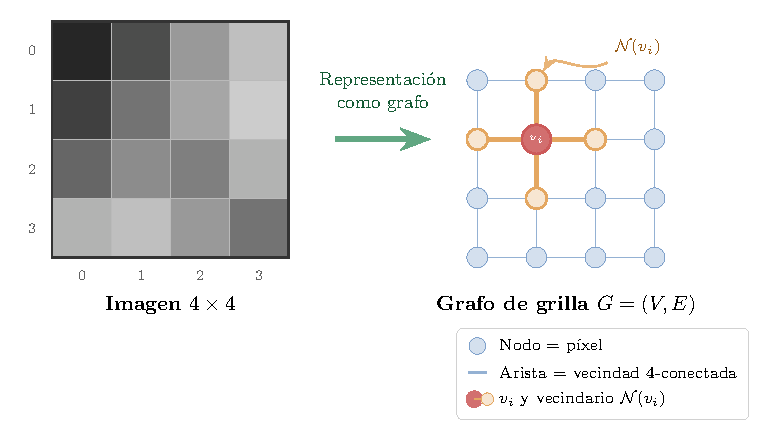
\includegraphics[width=0.85\textwidth]{images/image_as_graph}
	\caption[Imagen como grafo de grilla regular]{Una imagen puede representarse como un grafo de grilla regular con conectividad 4: cada píxel es un nodo y las aristas conectan píxeles vecinos horizontal y verticalmente. La vecindad $\mathcal{N}(v_i)$ corresponde exactamente al soporte del kernel convolucional.}
	\label{fig:image_as_graph}
\end{figure}

\begin{example}[Construcción Explícita: Imagen 3×3 como Grafo]\label{ex:imagen_3x3_grafo}
Consideremos una imagen RGB de tamaño $3 \times 3$ con 3 canales de color. La transformación a grafo procede en tres pasos:

\textbf{Paso 1: Identificación de nodos}. Cada píxel $(i,j)$ se mapea a un nodo $v_{i,j}$ del grafo:
\[
V = \{v_{0,0}, v_{0,1}, v_{0,2}, v_{1,0}, v_{1,1}, v_{1,2}, v_{2,0}, v_{2,1}, v_{2,2}\}
\]
con $|V| = 9$ nodos.

\textbf{Paso 2: Construcción de aristas}. Para 4-conectividad, conectamos píxeles adyacentes horizontal y verticalmente:
\begin{align}
E = \{&(v_{0,0}, v_{0,1}), (v_{0,1}, v_{0,2}), \quad \text{(fila 0)} \\
    &(v_{1,0}, v_{1,1}), (v_{1,1}, v_{1,2}), \quad \text{(fila 1)} \\
    &(v_{2,0}, v_{2,1}), (v_{2,1}, v_{2,2}), \quad \text{(fila 2)} \\
    &(v_{0,0}, v_{1,0}), (v_{1,0}, v_{2,0}), \quad \text{(columna 0)} \\
    &(v_{0,1}, v_{1,1}), (v_{1,1}, v_{2,1}), \quad \text{(columna 1)} \\
    &(v_{0,2}, v_{1,2}), (v_{1,2}, v_{2,2}) \} \quad \text{(columna 2)}
\end{align}
Obtenemos $|E| = 12$ aristas no dirigidas.

\textbf{Paso 3: Asignación de características}. Cada nodo $v_{i,j}$ recibe un vector de características $\mathbf{x}_{i,j} \in \mathbb{R}^3$ correspondiente a los valores RGB del píxel $(i,j)$:
\[
X = \begin{bmatrix} \mathbf{x}_{0,0}^T \\ \mathbf{x}_{0,1}^T \\ \vdots \\ \mathbf{x}_{2,2}^T \end{bmatrix} \in \mathbb{R}^{9 \times 3}
\]

La matriz de adyacencia $A \in \{0,1\}^{9 \times 9}$ tiene la forma block-tridiagonal característica de grillas regulares.
\end{example}

\textbf{Propiedades Especiales de Grafos Grilla.} Los grafos grilla derivados de imágenes poseen propiedades estructurales únicas:
\begin{enumerate}
    \item \textbf{Regularidad}: Grado casi constante ($\deg(v) = 4$ excepto en bordes)
    \item \textbf{Estructura espacial}: Posiciones $(i,j)$ definen un embedding natural en $\mathbb{R}^2$
    \item \textbf{Simetría}: Invarianza a traslaciones discretas
    \item \textbf{Espectro predecible}: Los eigenvalores del Laplaciano son conocidos analíticamente
\end{enumerate}

Estas propiedades hacen que las CNNs sean especialmente efectivas en grillas, pero también limitan su aplicabilidad a grafos generales.

\subsection[CNNs como GNNs en Grillas Regulares]{\glspl{CNN} como \glspl{GNN} en Grillas Regulares}\label{subsec:cnns_como_gnns_grillas}

\begin{theorem}[\gls{CNN} es un Caso Especial de \gls{GNN}]\label{thm:cnn_caso_especial_gnn}
Una \gls{CNN} 2D es exactamente equivalente a una \gls{GNN} donde:
\begin{itemize}
	\item \textbf{Grafo}: Grilla regular \(G = (\mathbb{Z}^2 \cap \Omega, E)\)
	\item \textbf{Vértices}: Píxeles en posiciones \((i,j)\)
	\item \textbf{Aristas}: Conectividad 4 u 8 vecinos
	\item \textbf{Pesos}: Compartidos según posición relativa (kernel)
\end{itemize}
\end{theorem}

\begin{proof}
La equivalencia se establece mediante la correspondencia natural:
\begin{enumerate}
	\item Cada píxel \((i,j)\) corresponde a un nodo \(v_{i,j}\) en el grafo
	\item Las conexiones espaciales definen las aristas: \((v_{i,j}, v_{i',j'}) \in E\) si y solo si \(|i-i'| + |j-j'| \leq 1\)
	\item El kernel convolucional \(K\) determina los pesos de las aristas según la distancia relativa
	\item La operación de agregación en \glspl{GNN} se reduce exactamente a la convolución 2D
\end{enumerate}
\end{proof}

\begin{definition}[Grilla como Grafo]\label{def:grilla_como_grafo}
Para imagen de tamaño \(H \times W\):
\begin{itemize}
	\item \(V = \{(i,j) : 0 \leq i < H, 0 \leq j < W\}\)
	\item \(E = \{((i,j), (i',j')) : |i-i'| + |j-j'| \leq 1\}\) (4-conectividad)
	\item Grado constante: \(\deg(v) = 4\) (excepto bordes)
\end{itemize}
\end{definition}

\begin{theorem}[Equivalencia Constructiva CNN-GNN]\label{thm:equivalencia_constructiva_cnn_gnn}
Dada una CNN con arquitectura de capas convolucionales $\{L_\ell\}_{\ell=1}^L$ operando sobre grillas $H \times W$, existe una construcción explícita de una GNN equivalente que produce salidas idénticas para toda entrada.

\textbf{Construcción}:
\begin{enumerate}
    \item \textbf{Grafo}: $G = (V, E)$ donde $V = \{(i,j) : 0 \leq i < H, 0 \leq j < W\}$ y
    \[
    E = \{((i,j), (i',j')) : |i-i'| + |j-j'| = 1\}
    \]

    \item \textbf{Características iniciales}: Para cada nodo $v_{i,j}$, asignar $h_{v_{i,j}}^{(0)} = x_{i,j}$ donde $x_{i,j}$ es el valor del píxel en $(i,j)$

    \item \textbf{Función de mensaje}: Para un kernel CNN $K \in \mathbb{R}^{k \times k \times c_{\text{in}} \times c_{\text{out}}}$, definir
    \[
    M_\ell(h_v^{(\ell)}, h_u^{(\ell)}, e_{vu}) = W_{v-u}^{(\ell)} h_u^{(\ell)}
    \]
    donde $W_{v-u}^{(\ell)} \in \mathbb{R}^{c_{\text{out}} \times c_{\text{in}}}$ es la submatriz del kernel correspondiente al desplazamiento $(v-u)$

    \item \textbf{Agregación}:
    \[
    m_v^{(\ell+1)} = \sum_{u \in \mathcal{N}(v)} M_\ell(h_v^{(\ell)}, h_u^{(\ell)}, e_{vu})
    \]

    \item \textbf{Actualización}:
    \[
    h_v^{(\ell+1)} = \sigma(m_v^{(\ell+1)} + b^{(\ell)})
    \]
    donde $\sigma$ es la función de activación y $b^{(\ell)}$ el sesgo
\end{enumerate}

Esta construcción garantiza que $h_v^{(\ell)} = y_{i,j}^{(\ell)}$ para todo nodo $v = (i,j)$ y capa $\ell$, donde $y_{i,j}^{(\ell)}$ es la activación de la CNN en la posición $(i,j)$ de la capa $\ell$.
\end{theorem}

\begin{proof}
Procederemos por inducción en la profundidad de la red.

\textbf{Caso base} ($\ell = 0$): Por construcción, $h_v^{(0)} = x_{i,j} = y_{i,j}^{(0)}$ para todo nodo $v = (i,j)$.

\textbf{Paso inductivo}: Supongamos que $h_v^{(\ell)} = y_{i,j}^{(\ell)}$ para todo $v = (i,j)$. Debemos mostrar que $h_v^{(\ell+1)} = y_{i,j}^{(\ell+1)}$.

Para la CNN, la salida en la posición $(i,j)$ de la capa $\ell+1$ es:
\begin{align}
y_{i,j}^{(\ell+1)} &= \sigma\left(\sum_{(u,v) \in \mathcal{K}} K_{u,v} \cdot x_{i+u,j+v}^{(\ell)} + b^{(\ell)}\right) \\
&= \sigma\left(\sum_{(i',j') \in \mathcal{N}(i,j)} K_{i'-i,j'-j} \cdot y_{i',j'}^{(\ell)} + b^{(\ell)}\right)
\end{align}

donde $\mathcal{K}$ es el soporte del kernel y $\mathcal{N}(i,j)$ el vecindario del píxel $(i,j)$.

Para la GNN, usando la construcción propuesta:
\begin{align}
h_v^{(\ell+1)} &= \sigma\left(\sum_{u \in \mathcal{N}(v)} W_{v-u}^{(\ell)} h_u^{(\ell)} + b^{(\ell)}\right) \\
&= \sigma\left(\sum_{(i',j') \in \mathcal{N}(i,j)} K_{i'-i,j'-j} \cdot h_{(i',j')}^{(\ell)} + b^{(\ell)}\right) \\
&\overset{\text{H.I.}}{=} \sigma\left(\sum_{(i',j') \in \mathcal{N}(i,j)} K_{i'-i,j'-j} \cdot y_{i',j'}^{(\ell)} + b^{(\ell)}\right) \\
&= y_{i,j}^{(\ell+1)}
\end{align}

donde usamos la hipótesis inductiva (H.I.) en la tercera igualdad. $\square$
\end{proof}

\begin{example}[Verificación Numérica: Kernel 3×3 Sobel]\label{ex:verificacion_numerica_sobel}
Consideremos el kernel Sobel horizontal:
\[
K = \begin{bmatrix} -1 & 0 & 1 \\ -2 & 0 & 2 \\ -1 & 0 & 1 \end{bmatrix}
\]

Aplicado a la imagen $3 \times 3$:
\[
I = \begin{bmatrix} 0 & 1 & 2 \\ 0 & 1 & 2 \\ 0 & 1 & 2 \end{bmatrix}
\]

\textbf{Método CNN}: La convolución en el píxel central $(1,1)$ produce:
\begin{align}
y_{1,1} &= -1 \cdot 0 + 0 \cdot 1 + 1 \cdot 2 \\
        &\quad + (-2) \cdot 0 + 0 \cdot 1 + 2 \cdot 2 \\
        &\quad + (-1) \cdot 0 + 0 \cdot 1 + 1 \cdot 2 \\
        &= 0 + 2 + 0 + 4 + 0 + 2 = 8
\end{align}

\textbf{Método GNN}: Construimos el grafo con $v_{1,1}$ conectado a sus 8 vecinos. Los mensajes son:
\begin{align}
m_{1,1} &= K_{-1,-1} \cdot h_{0,0} + K_{-1,0} \cdot h_{0,1} + K_{-1,1} \cdot h_{0,2} \\
        &\quad + K_{0,-1} \cdot h_{1,0} + K_{0,1} \cdot h_{1,2} \\
        &\quad + K_{1,-1} \cdot h_{2,0} + K_{1,0} \cdot h_{2,1} + K_{1,1} \cdot h_{2,2} \\
        &= (-1)(0) + (0)(1) + (1)(2) + (-2)(0) + (2)(2) \\
        &\quad + (-1)(0) + (0)(1) + (1)(2) = 8
\end{align}

Ambos métodos producen el resultado idéntico $y_{1,1} = 8$, verificando la equivalencia.
\end{example}

\subsection{Equivalencia Convolución-Message Passing}\label{subsec:equivalencia_conv_mp}

\begin{theorem}[Equivalencia Fundamental]\label{thm:equivalencia_fundamental_conv_mp}
La operación de convolución 2D:
\[
y_{i,j} = \sum_{(u,v) \in \mathcal{N}} K_{u,v} \cdot x_{i+u,j+v}
\]

es exactamente equivalente a message passing en la grilla:
\[
m_{(i,j)} = \sum_{(i',j') \in N(i,j)} K_{i'-i,j'-j} \cdot x_{i',j'}
\]

donde \(N(i,j)\) son los vecinos del píxel \((i,j)\).
\end{theorem}

\begin{proof}
La convolución suma sobre un vecindario fijo relativo al píxel central.
En la grilla regular, este vecindario corresponde exactamente a los
vecinos en el grafo con pesos determinados por la posición relativa.
Los pesos \(K_{u,v}\) del kernel corresponden a los mensajes ponderados. \(\square\)
\end{proof}

\begin{figure}[htbp]
	\centering
	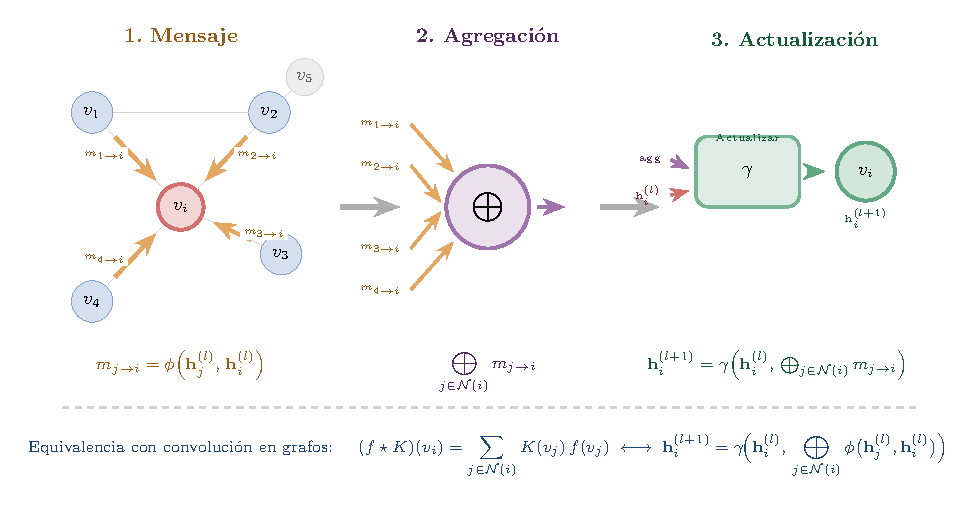
\includegraphics[width=0.90\textwidth]{images/conv_message_passing}
	\caption[Equivalencia convolución-message passing]{Equivalencia entre convolución y message passing: los tres pasos fundamentales (mensaje, agregación, actualización) corresponden exactamente a la operación convolucional cuando el grafo es una grilla regular.}
	\label{fig:conv_message_passing}
\end{figure}

\begin{example}[Demostración Paso a Paso: Convolución = Message Passing]\label{ex:paso_a_paso_conv_mp}
Consideremos una señal 1D $f = [1, 3, 2, 4]$ y un kernel $K = [0.5, 1, 0.5]$ (filtro de suavizado).

\textbf{Interpretación como convolución}:
\begin{align}
(f * K)[1] &= 0.5 \cdot f[0] + 1 \cdot f[1] + 0.5 \cdot f[2] \\
           &= 0.5 \cdot 1 + 1 \cdot 3 + 0.5 \cdot 2 = 4.5
\end{align}

\textbf{Interpretación como message passing}:
Construimos un grafo lineal $v_0 \leftrightarrow v_1 \leftrightarrow v_2 \leftrightarrow v_3$ con características iniciales $h_{v_i}^{(0)} = f[i]$.

Los mensajes recibidos por el nodo $v_1$ son:
\begin{itemize}
    \item Desde $v_0$: $m_{v_1 \leftarrow v_0} = W_{-1} \cdot h_{v_0}^{(0)} = 0.5 \cdot 1 = 0.5$
    \item Auto-mensaje: $m_{v_1 \leftarrow v_1} = W_0 \cdot h_{v_1}^{(0)} = 1 \cdot 3 = 3$
    \item Desde $v_2$: $m_{v_1 \leftarrow v_2} = W_{+1} \cdot h_{v_2}^{(0)} = 0.5 \cdot 2 = 1$
\end{itemize}

La agregación produce:
\[
m_{v_1}^{(1)} = \sum_{u \in \mathcal{N}(v_1)} m_{v_1 \leftarrow u} = 0.5 + 3 + 1 = 4.5
\]

Nuevamente, ambos enfoques producen el mismo resultado: $4.5$.
\end{example}

\textbf{Conexión con el Marco MPNN Unificado.} La equivalencia convolución-message passing establecida en esta sección es un caso especial del marco de \textit{Message Passing Neural Networks} (\glspl{MPNN}) introducido en la \autoref{def:mpnn_unificador} del \autoref{ch:gdl}.

Específicamente, las CNNs corresponden a MPNNs con:
\begin{itemize}
    \item \textbf{Grafo fijo}: Grilla regular con conectividad local
    \item \textbf{Función de mensaje}: $M_\ell(h_v, h_u, e_{vu}) = W_{v-u}^{(\ell)} h_u$ (dependencia solo del desplazamiento relativo)
    \item \textbf{Agregación}: Suma no ponderada $m_v = \sum_{u \in \mathcal{N}(v)} M_\ell(\cdot)$
    \item \textbf{Actualización}: $U_\ell(h_v, m_v) = \sigma(m_v + b^{(\ell)})$
\end{itemize}

Esta formulación revela que la restricción fundamental de las CNNs es la \textbf{compartición de pesos basada en posición relativa} ($W_{v-u}$), que solo tiene sentido en dominios con estructura de traslación. Para grafos generales sin tal estructura, necesitamos funciones de mensaje más flexibles, como se explora en la \autoref{subsec:message_passing_unificador} del \autoref{ch:gdl}.

\begin{proposition}[Complejidad Computacional CNN vs GNN en Grillas]\label{prop:complejidad_cnn_vs_gnn_grilla}
Para una imagen de tamaño $H \times W$ con $C$ canales y kernel $k \times k$:
\begin{itemize}
    \item \textbf{CNN estándar}: $O(H \cdot W \cdot k^2 \cdot C)$ operaciones
    \item \textbf{GNN en grilla}: $O(|E| \cdot C) = O(4HW \cdot C)$ operaciones (para 4-conectividad)
\end{itemize}

Cuando $k$ es pequeño (típicamente $k \in \{3, 5, 7\}$), ambas complejidades son equivalentes: $O(HWC)$. Sin embargo, la formulación de GNN revela que la complejidad depende fundamentalmente del número de aristas $|E|$, no del tamaño del kernel, proporcionando una perspectiva unificada para analizar eficiencia en diferentes topologías de grafos.
\end{proposition}

\begin{proof}
\textbf{CNN estándar}: La imagen tiene $H \cdot W$ posiciones espaciales. En cada posición, el kernel $k \times k$ realiza $k^2$ multiplicaciones sobre cada uno de los $C$ canales, dando un total de $O(H \cdot W \cdot k^2 \cdot C)$ operaciones.

\textbf{GNN en grilla}: Cada nodo (píxel) tiene a lo sumo 4 vecinos en conectividad 4 (arriba, abajo, izquierda, derecha), luego $|E| = O(4HW)$. El paso de mensajes procesa $C$ canales por arista, resultando en $O(4HW \cdot C) = O(|E| \cdot C)$ operaciones.
\end{proof}

\textbf{Perspectiva Dual: Espacial vs. Espectral.} La equivalencia establecida en esta sección admite dos interpretaciones complementarias:

\textbf{Perspectiva espacial}: La convolución agrega información de vecinos locales con pesos compartidos determinados por la posición relativa. Esta es la formulación natural de las CNNs.

\textbf{Perspectiva espectral}: Como se desarrolló en la \autoref{sec:analisis_armonico}, la convolución corresponde a multiplicación en el dominio de Fourier. Para grillas regulares, los eigenvectores del Laplaciano son exactamente las bases de Fourier discretas, estableciendo la conexión con la \autoref{def:convolucion_espectral_grafos}.

Esta dualidad espacial-espectral es fundamental: las CNNs clásicas operan en el dominio espacial por eficiencia computacional, mientras que las formulaciones espectrales proporcionan las herramientas teóricas para generalizar a grafos arbitrarios mediante la aproximación de Chebyshev (\autoref{ex:chebyshev_aproximacion}).

\subsection{Laplaciano de Grilla y Filtros}\label{subsec:laplaciano_grilla_filtros}

\begin{definition}[Laplaciano Discreto en Grilla 2D]\label{def:laplaciano_discreto_grilla}
El operador Laplaciano en una grilla:
\[
\mathcal{L} = D - A
\]
donde \(D\) es la matriz de grados y \(A\) la matriz de adyacencia.

Para grilla 2D con 4-conectividad:
\begin{align}
\mathcal{L}_{(i,j),(i,j)} &= 4 \\
\mathcal{L}_{(i,j),(i \pm 1,j)} = \mathcal{L}_{(i,j),(i,j \pm 1)} &= -1
\end{align}
\end{definition}

\begin{example}[Kernel Laplaciano como Filtro CNN]
El Laplaciano discreto corresponde al kernel:
\[
K = \begin{bmatrix}
 0 & -1 &  0 \\
-1 &  4 & -1 \\
 0 & -1 &  0
\end{bmatrix}
\]
Este es un detector de bordes clásico en procesamiento de imágenes, y su interpretación espectral como filtro paso-alto se formaliza en el \autoref{thm:cnns_filtros_espectrales_grillas}.
\end{example}

\begin{proposition}[Eigenvalores del Laplaciano en Grilla Rectangular]\label{prop:eigenvalores_laplaciano_grilla}
Para una grilla 2D de tamaño $n_1 \times n_2$ con condiciones de frontera periódicas, los eigenvalores del Laplaciano son:
\begin{equation}
\lambda_{k_1,k_2} = 4 - 2\cos\!\left(\frac{2\pi k_1}{n_1}\right) - 2\cos\!\left(\frac{2\pi k_2}{n_2}\right), \quad 0 \leq k_i < n_i
\end{equation}
con eigenvectores $\phi_{k_1,k_2}(i,j) = \frac{1}{\sqrt{n_1 n_2}} e^{2\pi \imath(k_1 i/n_1 + k_2 j/n_2)}$, que son exactamente las bases de Fourier discretas.
\end{proposition}

\begin{proof}
Para condiciones de frontera periódicas, las funciones $\phi_{k_1,k_2}$ satisfacen $\phi_{k_1,k_2}(i + n_1, j) = \phi_{k_1,k_2}(i,j)$. Aplicando el Laplaciano:
\begin{align}
(\mathcal{L}\phi_{k_1,k_2})(i,j) &= 4\phi_{k_1,k_2}(i,j) - \phi_{k_1,k_2}(i+1,j) - \phi_{k_1,k_2}(i-1,j) - \phi_{k_1,k_2}(i,j+1) - \phi_{k_1,k_2}(i,j-1) \\
&= \left(4 - e^{2\pi \imath k_1/n_1} - e^{-2\pi \imath k_1/n_1} - e^{2\pi \imath k_2/n_2} - e^{-2\pi \imath k_2/n_2}\right)\phi_{k_1,k_2}(i,j) \\
&= \left(4 - 2\cos\!\left(\frac{2\pi k_1}{n_1}\right) - 2\cos\!\left(\frac{2\pi k_2}{n_2}\right)\right)\phi_{k_1,k_2}(i,j)
\end{align}
confirmando que $\phi_{k_1,k_2}$ es eigenvector con eigenvalor $\lambda_{k_1,k_2}$.
\end{proof}

\begin{remark}[Interpretación Frecuencial de los Eigenvalores]\label{rem:interpretacion_frecuencial_eigenvalores}
Los eigenvalores del Laplaciano en la grilla admiten una interpretación frecuencial directa:
\begin{itemize}
    \item \textbf{Frecuencia cero}: $\lambda_{0,0} = 0$ corresponde a la componente DC (señal constante), el eigenvector $\phi_{0,0} = 1/\sqrt{n_1 n_2}$ es uniforme.
    \item \textbf{Frecuencias bajas}: eigenvalores pequeños ($k_1, k_2$ cercanos a 0) corresponden a variaciones suaves en la grilla. Un filtro paso-bajo selecciona estos modos.
    \item \textbf{Frecuencias altas}: eigenvalores grandes (cercanos a $\lambda_{\max} = 8$ para la grilla cuadrada) corresponden a variaciones rápidas. Un filtro paso-alto (como el Laplaciano) selecciona estos modos.
    \item \textbf{Máxima frecuencia}: $\lambda_{n/2,n/2} = 8$ corresponde a la máxima oscilación posible (patrón de tablero de ajedrez $(-1)^{i+j}$).
\end{itemize}
\end{remark}

\begin{example}[Filtros Paso-Bajo y Paso-Alto en la Grilla]\label{ex:filtros_paso_bajo_alto}
Los filtros clásicos de procesamiento de imágenes tienen interpretaciones espectrales precisas:

\textbf{Filtro de suavizado (media $3 \times 3$)}: El kernel $K_{\text{media}} = \frac{1}{9}\begin{bsmallmatrix} 1 & 1 & 1 \\ 1 & 1 & 1 \\ 1 & 1 & 1 \end{bsmallmatrix}$ actúa como filtro paso-bajo, atenuando las componentes de alta frecuencia (eigenvalores grandes del Laplaciano) mientras preserva las componentes de baja frecuencia.

\textbf{Filtro de enfoque (sharpening)}: El kernel $K_{\text{sharp}} = \begin{bsmallmatrix} 0 & -1 & 0 \\ -1 & 5 & -1 \\ 0 & -1 & 0 \end{bsmallmatrix} = I + \mathcal{L}$ amplifica las componentes de alta frecuencia, donde $I$ preserva la señal original y $\mathcal{L}$ añade las diferencias locales.

En el dominio espectral, la respuesta de estos filtros es:
\begin{align}
\hat{K}_{\text{media}}(\lambda) &\approx 1 - c\lambda + O(\lambda^2) \quad \text{(paso-bajo)} \\
\hat{K}_{\text{sharp}}(\lambda) &= 1 + \lambda \quad \text{(amplificación de altas frecuencias)}
\end{align}
\end{example}

\begin{proposition}[Conexión entre Laplaciano Discreto y Continuo]\label{prop:laplaciano_discreto_continuo}
El Laplaciano discreto en grilla es una aproximación por diferencias finitas del Laplaciano continuo $\Delta f = \frac{\partial^2 f}{\partial x^2} + \frac{\partial^2 f}{\partial y^2}$. Para una función $f$ suficientemente suave definida en la grilla con paso $h$:
\[
(\mathcal{L}f)_{i,j} = h^2 \Delta f(ih, jh) + O(h^4)
\]
\end{proposition}

\begin{proof}
Por el desarrollo de Taylor de segundo orden:
\begin{align}
f(i+1,j) &= f(i,j) + h f_x + \frac{h^2}{2}f_{xx} + \frac{h^3}{6}f_{xxx} + O(h^4) \\
f(i-1,j) &= f(i,j) - h f_x + \frac{h^2}{2}f_{xx} - \frac{h^3}{6}f_{xxx} + O(h^4)
\end{align}
Sumando: $f(i+1,j) + f(i-1,j) = 2f(i,j) + h^2 f_{xx} + O(h^4)$. Análogamente para la dirección $j$. Por tanto:
\[
4f(i,j) - f(i+1,j) - f(i-1,j) - f(i,j+1) - f(i,j-1) = -h^2(f_{xx} + f_{yy}) + O(h^4) = -h^2 \Delta f + O(h^4)
\]
lo que demuestra que $(\mathcal{L}f)_{i,j} = -h^2 \Delta f + O(h^4)$, con signo negativo consistente con la convención $\mathcal{L} = D - A$ (Laplaciano semidefinido positivo).
\end{proof}

\subsection{Generalización Espectral}\label{subsec:generalizacion_espectral}

\begin{theorem}[CNNs como Filtros Espectrales en Grillas]\label{thm:cnns_filtros_espectrales_grillas}
Los filtros convolucionales pueden interpretarse como filtros 
espectrales sobre el Laplaciano de la grilla:
\[
h_\theta * f = \sum_k h_\theta(\lambda_k)\langle f, \phi_k\rangle\phi_k
\]
donde \(\{\lambda_k, \phi_k\}\) son eigenvalores/eigenvectores del Laplaciano de grilla.
\end{theorem}

\begin{proof}
Sea $\mathcal{L} = U \Lambda U^T$ la descomposición espectral del Laplaciano de la grilla, con $\Lambda = \operatorname{diag}(\lambda_0, \ldots, \lambda_{n-1})$ y $U = [\phi_0 | \cdots | \phi_{n-1}]$. Un filtro convolucional con kernel $h_\theta$ actúa sobre la señal $f$ en el dominio espacial como $(h_\theta * f)(i) = \sum_j h_\theta(i-j) f(j)$. En el dominio espectral, por el teorema de convolución, esto equivale a $\widehat{h_\theta * f}(k) = \hat{h}_\theta(k) \cdot \hat{f}(k)$, donde $\hat{f}(k) = \langle f, \phi_k \rangle$. Definiendo $h_\theta(\lambda_k) := \hat{h}_\theta(k)$, la señal filtrada se reconstruye como:
\[
(h_\theta * f)(i) = \sum_k h_\theta(\lambda_k) \langle f, \phi_k \rangle \phi_k(i)
\]
que es exactamente la convolución espectral del enunciado.
\end{proof}

\begin{proposition}[De Grillas Regulares a Grafos Arbitrarios]\label{prop:grillas_a_grafos}
La generalización natural de CNNs a grafos arbitrarios es:
\begin{enumerate}
	\item Reemplazar la grilla regular por un grafo general
	\item Reemplazar el kernel espacial por funciones del Laplaciano
	\item Mantener la idea de agregación local de información
\end{enumerate}
\end{proposition}

\begin{proof}
La generalización se justifica por la equivalencia espectral establecida en el \autoref{thm:cnns_filtros_espectrales_grillas}: dado que los filtros convolucionales en grillas son funciones del Laplaciano $h_\theta(\mathcal{L})$, y el Laplaciano $\mathcal{L} = D - A$ está definido para cualquier grafo (no solo grillas), la formulación $h_\theta(\mathcal{L})f = \sum_k h_\theta(\lambda_k)\langle f, \phi_k \rangle \phi_k$ se extiende directamente a grafos arbitrarios. Los tres pasos del enunciado corresponden a: (1) reemplazar la grilla por un grafo con su propia matriz de adyacencia, (2) usar la descomposición espectral del nuevo Laplaciano como base funcional, y (3) preservar la localidad espacial mediante filtros polinomiales de grado $K$ que operan en vecindarios de radio $K$.
\end{proof}

La convolución espectral en grafos (\autoref{def:convolucion_espectral_grafos}) permite trasladar la operación convolucional al dominio espectral: $\text{conv}_\theta \star x = U g_\theta(\Lambda) U^T x$, donde $\mathcal{L} = U\Lambda U^T$ es la descomposición espectral del Laplaciano y $g_\theta$ es el filtro entrenable.

\subsubsection{Análisis Espectral Detallado}

El análisis espectral proporciona las herramientas matemáticas fundamentales para entender y diseñar convoluciones sobre grafos como generalización de las \glspl{CNN} clásicas.

La descomposición espectral del Laplaciano normalizado $\mathcal{L} = U \Lambda U^T$ y la transformada de Fourier en grafos $\hat{f} = U^T f$ (\autoref{def:transformada_fourier_grafos}, \autoref{ch:gdl}) permiten definir filtros espectrales como funciones $g: [0,2] \to \mathbb{R}$ que actúan sobre señales mediante $(g \star f) = U g(\Lambda) U^T f$. Un filtro $K$-localizado concentra su soporte en los primeros $K$ eigenvalores, induciendo operaciones locales con complejidad $O(K|V|)$ que generalizan los kernels locales de las \glspl{CNN}.

La aproximación por polinomios de Chebyshev (\autoref{ex:chebyshev_aproximacion}) permite hacer computacionalmente tratables estas convoluciones espectrales. La recurrencia del \autoref{thm:eficiencia_chebyshev} reduce la complejidad a $O(K|E|)$ sin requerir la diagonalización del Laplaciano. Véase \citep{defferrard2017convolutionalneuralnetworksgraphs} para la formulación original en el contexto de \glspl{GNN}.

\textbf{Puente Conceptual: Análisis Armónico Unificador.} El análisis armónico desarrollado en la \autoref{sec:analisis_armonico} proporciona el lenguaje matemático para unificar CNNs y GNNs:
\begin{enumerate}
    \item \textbf{Dominio euclidiano}: Transformada de Fourier clásica (\autoref{def:transformada_fourier_continua})
    \item \textbf{Grillas discretas}: DFT y FFT (Definiciones~\ref{def:dft}, \ref{def:fft})
    \item \textbf{Grupos finitos/compactos}: Transformada de Fourier en grupos (Ecuación~\ref{eq:fourier_grupo_finito})
    \item \textbf{Grafos generales}: Transformada de Fourier en grafos (\autoref{def:transformada_fourier_grafos}, \autoref{ch:gdl})
\end{enumerate}

Cada nivel generaliza el anterior mientras preserva la intuición fundamental: las frecuencias bajas capturan estructura suave/global, las frecuencias altas capturan detalles/variaciones locales.

\subsubsection{De CNNs Espectrales a Graph Neural Networks}

La teoría espectral anterior establece el puente formal entre las \glspl{CNN} tradicionales y las redes de grafos, demostrando que ambas son casos especiales del mismo principio matemático fundamental.

\begin{theorem}[Conexión Fundamental CNN-GNN]\label{thm:conexion_fundamental_cnn_gnn}
Toda \gls{CNN} puede representarse exactamente como una \gls{GNN} espectral sobre una grilla regular, donde:
\begin{enumerate}
    \item El grafo $G = (V, E)$ representa la estructura de píxeles con $V = \{(i,j) : 1 \leq i,j \leq n\}$
    \item La conectividad $E$ está determinada por la vecindad espacial
    \item Los filtros espectrales corresponden a kernels convolucionales via transformada de Fourier discreta
\end{enumerate}
\end{theorem}

\begin{proof}[Esbozo de demostración]
Para una grilla 2D de tamaño $n \times n$, consideremos el grafo $G$ donde cada píxel $(i,j)$ es un nodo y las aristas conectan píxeles adyacentes. El Laplaciano de este grafo tiene la forma:
\[
\mathcal{L}_{(i,j),(i',j')} = \begin{cases}
4 & \text{si } (i,j) = (i',j') \\
-1 & \text{si } |i-i'| + |j-j'| = 1 \\
0 & \text{en caso contrario}
\end{cases}
\]

Sus eigenvectores son exactamente las funciones de Fourier discretas bidimensionales:
\[
\phi_{k,\ell}(i,j) = \frac{1}{n} e^{2\pi \imath (ki + \ell j)/n}
\]

Por tanto, la convolución espacial $f * g$ corresponde exactamente a la multiplicación espectral $\hat{f} \odot \hat{g}$ en el dominio de frecuencias del grafo. $\square$
\end{proof}

\subsubsection{Implementaciones Computacionalmente Eficientes}

El trabajo pionero de \citet{defferrard2017convolutionalneuralnetworksgraphs} resolvió el problema computacional de las convoluciones espectrales mediante aproximaciones polinomiales de Chebyshev.

\begin{definition}[ChebNet: Convolución de Chebyshev]\label{def:chebnet}
Un filtro espectral aproximado por polinomios de Chebyshev de orden $K$ se define como:
\[
g_\theta(\Lambda) = \sum_{k=0}^{K} \theta_k T_k(\tilde{\Lambda})
\]
donde $T_k$ son los polinomios de Chebyshev de primera especie, $\tilde{\Lambda} = 2\Lambda/\lambda_{\max} - I$ es el Laplaciano escalado, y $\theta_k$ son parámetros entrenables.
\end{definition}

\begin{theorem}[Localización de Filtros de Chebyshev]\label{thm:localizacion_chebyshev}
Un filtro de Chebyshev de orden $K$ es estrictamente $K$-localizado: la respuesta en el nodo $i$ depende únicamente de nodos a distancia máxima $K$ de $i$ en el grafo.
\end{theorem}

\begin{proof}
Un polinomio de Chebyshev $T_k$ de grado $k$ satisface $T_k(\tilde{\mathcal{L}}) = 2\tilde{\mathcal{L}} T_{k-1}(\tilde{\mathcal{L}}) - T_{k-2}(\tilde{\mathcal{L}})$. Puesto que $\tilde{\mathcal{L}}_{ij} \neq 0$ solo si los nodos $i$ y $j$ son adyacentes (distancia 1), la multiplicación por $\tilde{\mathcal{L}}$ extiende el soporte de una señal en exactamente un salto. Así, $T_1(\tilde{\mathcal{L}})f$ depende de vecinos a distancia $\leq 1$, y por inducción, $T_k(\tilde{\mathcal{L}})f$ en el nodo $i$ depende únicamente de nodos a distancia $\leq k$. Como el filtro es $g_\theta(\tilde{\mathcal{L}}) = \sum_{k=0}^K \theta_k T_k(\tilde{\mathcal{L}})$, la respuesta en cada nodo depende de nodos a distancia $\leq K$.
\end{proof}

La evaluación eficiente de estos filtros se obtiene mediante la recurrencia de Chebyshev establecida en el \autoref{thm:eficiencia_chebyshev}, que permite calcular $g_\theta(\tilde{\mathcal{L}}) \mathbf{x}$ en tiempo $O(K|\mathcal{E}|)$ sin diagonalizar el Laplaciano, con solo $O(K)$ parámetros entrenables independientes del tamaño del grafo.

Esta mejora computacional elimina la necesidad de calcular la descomposición espectral completa, haciendo que las \glspl{GNN} espectrales sean prácticas para grafos de gran escala.

\subsubsection{Ejemplos Concretos de Traducción CNN $\rightarrow$ GNN}

\begin{example}[Kernel Sobel como Filtro Espectral]
El kernel de detección de bordes Sobel:
\[
K_{\text{Sobel}} = \begin{bmatrix} -1 & 0 & 1 \\ -2 & 0 & 2 \\ -1 & 0 & 1 \end{bmatrix}
\]

En el dominio espectral del grafo grilla, este filtro corresponde a:
\[
\hat{g}(\lambda_{k,\ell}) = |\sin(2\pi k/n)| \cdot \text{función de frecuencia vertical}
\]

Este ejemplo demuestra cómo los filtros de detección de características en \glspl{CNN} tienen interpretaciones espectrales naturales en grafos.
\end{example}

\begin{example}[Pooling como Coarsening de Grafo]
El max-pooling $2 \times 2$ de \glspl{CNN} corresponde a:
\begin{enumerate}
    \item \textbf{Agrupamiento}: Particionar cada bloque $2 \times 2$ de píxeles
    \item \textbf{Agregación}: Aplicar función max sobre cada partición
    \item \textbf{Nuevo grafo}: Construir grafo coarser con $n/4$ nodos
\end{enumerate}

Esto generaliza a grafos arbitrarios mediante algoritmos de coarsening algebraico que preservan la estructura espectral local.
\end{example}

\subsection{Implicaciones y Transición}\label{subsec:implicaciones_transicion_cnn_gnn}

Esta equivalencia \gls{CNN}-\gls{GNN} tiene implicaciones profundas que trascienden la mera analogía matemática y proporcionan un marco conceptual para entender las limitaciones y extensiones de las arquitecturas convolucionales.

\subsubsection{Unificación Conceptual}

\begin{proposition}[Principios Compartidos CNN-GNN]\label{prop:principios_compartidos}
Las \glspl{CNN} y \glspl{GNN} comparten tres principios arquitectónicos fundamentales:
\begin{enumerate}
    \item \textbf{Localidad}: Agregación de información desde vecindarios locales
    \item \textbf{Compartición de pesos}: Reutilización de parámetros a través del dominio
    \item \textbf{Composición jerárquica}: Construcción de representaciones multi-escala
\end{enumerate}
\end{proposition}

\begin{proof}
(1) \textit{Localidad}: En una CNN, cada capa convolucional agrega información de un vecindario de tamaño $k$ (el kernel). En una GNN, el paso de message passing agrega información de los vecinos 1-hop $\mathcal{N}(i)$. En ambos casos, la operación es local y está determinada por la estructura de adyacencia del dominio.

(2) \textit{Compartición de pesos}: En una CNN, el mismo kernel se aplica en todas las posiciones espaciales. En una GNN, la misma función de mensaje $\phi$ y de actualización $\gamma$ se aplica en todos los nodos. En ambos casos, los parámetros son independientes de la posición.

(3) \textit{Composición jerárquica}: En una CNN, las operaciones de pooling reducen la resolución espacial creando representaciones multi-escala. En una GNN, los algoritmos de coarsening (como Graclus o DiffPool) colapsan nodos, produciendo grafos progresivamente más pequeños con representaciones de nivel superior.
\end{proof}

\subsubsection{Limitaciones de CNNs y Superación mediante GNNs}

\begin{remark}[Limitaciones Estructurales de CNNs]\label{rem:limitaciones_estructurales_cnns}
Las \glspl{CNN} tradicionales presentan las siguientes restricciones fundamentales, consecuencia directa de su equivarianza exclusiva a traslaciones (\autoref{theorem:convolution_translation_equivariance}):
\begin{enumerate}
    \item \textbf{Dependencia de grilla regular}: Requieren estructura euclidiana fija
    \item \textbf{Rigidez topológica}: No pueden procesar directamente dominios irregulares
    \item \textbf{Pérdida de información geométrica}: La representación euclidiana puede destruir relaciones intrínsecas
    \item \textbf{Escalabilidad limitada}: Complejidad cuadrática con resolución para estructuras no locales
\end{enumerate}
\end{remark}

\begin{example}[Casos donde CNNs Fallan y GNNs Triunfan]
\leavevmode
\begin{enumerate}
    \item \textbf{Análisis molecular}: Las moléculas son grafos naturalmente, no grillas
    \item \textbf{Redes sociales}: La conectividad social no respeta geometría euclidiana
    \item \textbf{Mallas 3D}: Superficies complejas con topología variable
    \item \textbf{Sistemas de transporte}: Redes con conectividad no-uniforme
\end{enumerate}
\end{example}

\subsubsection{Transferencia Bidireccional de Técnicas}

\begin{proposition}[Transferibilidad de Innovaciones]
Técnicas desarrolladas para \glspl{CNN} se adaptan naturalmente a \glspl{GNN} y viceversa:
\begin{itemize}
    \item \textbf{CNN $\rightarrow$ GNN}: Pooling, dropout, batch normalization, skip connections
    \item \textbf{GNN $\rightarrow$ CNN}: Attention mechanisms, adaptive pooling, graph-inspired regularization
\end{itemize}
\end{proposition}

\begin{proof}
La transferibilidad se fundamenta en la equivalencia estructural establecida en el \autoref{thm:conexion_fundamental_cnn_gnn}. Las técnicas de CNN que dependen solo de operaciones locales y compartición de pesos se transfieren a GNNs porque ambas arquitecturas comparten estos principios (véase \autoref{prop:principios_compartidos}): pooling corresponde a coarsening de grafos, dropout se aplica a nodos/aristas, batch normalization se adapta por nodo, y skip connections preservan la estructura. En dirección inversa, los mecanismos de atención de GNNs (que ponderan vecinos adaptativamente) se transfieren a CNNs como atención espacial, y las técnicas de pooling adaptativo en grafos inspiran métodos de pooling no uniforme en imágenes.
\end{proof}

\subsubsection{Marco de Generalización Progresiva}

\begin{theorem}[Jerarquía de Generalización]\label{thm:jerarquia_generalizacion_cnn}
Las arquitecturas neuronales admiten la siguiente jerarquía de generalización:
\begin{align}
\text{Perceptron} &\subset \text{MLP} \subset \text{CNN (grilla)} \subset \text{CNN espectral} \nonumber \\
&\subset \text{GNN espectral} \subset \text{GNN espacial} \subset \text{MPNN general}
\end{align}
donde cada inclusión representa la relajación de una restricción arquitectónica específica.
\end{theorem}

\begin{corollary}[Poder Expresivo Creciente]\label{cor:poder_expresivo_creciente}
Cada nivel de la jerarquía anterior puede expresar estrictamente más funciones que los niveles anteriores, al costo de mayor complejidad computacional y riesgo de sobreajuste.
\end{corollary}

\begin{proof}
Cada inclusión en la jerarquía relaja una restricción arquitectónica específica: CNN $\subset$ CNN espectral relaja la localidad espacial del kernel, CNN espectral $\subset$ GNN espectral relaja la estructura de grilla regular, etc. La inclusión en cada caso es estricta porque la relajación permite expresar funciones que violan la restricción anterior. Por ejemplo, existen funciones equivariantes respecto al grupo de simetría del grafo que no pueden implementarse como convoluciones sobre grilla, pues la grilla impone simetrías de traslación que el grafo general no posee. El aumento en poder expresivo conlleva mayor complejidad computacional (más parámetros y operaciones por capa) y mayor riesgo de sobreajuste (espacio de hipótesis más grande con la misma cantidad de datos).
\end{proof}

\subsubsection{Interpretabilidad desde Perspectiva de Grafos}

\textbf{Nueva Interpretación de CNNs.} La perspectiva de grafos proporciona nuevas herramientas para interpretar \glspl{CNN}:
\begin{itemize}
    \item \textbf{Análisis espectral}: Entender filtros como funciones espectrales
    \item \textbf{Localización}: Cuantificar el campo receptivo usando distancias de grafo
    \item \textbf{Robustez}: Analizar estabilidad usando perturbaciones de grafo
    \item \textbf{Transferibilidad}: Evaluar generalización mediante propiedades espectrales
\end{itemize}

\subsubsection{Puente hacia Extensiones Geométricas}

Esta equivalencia fundamental \gls{CNN}-\gls{GNN} establece el fundamento conceptual para las extensiones geométricas que exploraremos:

\begin{definition}[Taxonomía de Extensiones Geométricas]\label{def:taxonomia_extensiones}
A partir de la base CNN-GNN, identificamos tres direcciones principales de generalización:
\begin{enumerate}
    \item \textbf{Convoluciones de Grupo}: Generalizar traslaciones a grupos de transformación más ricos
    \item \textbf{Convoluciones en Variedades}: Extender a dominios con curvatura no-trivial
    \item \textbf{Convoluciones Gauge}: Incorporar invarianzas gauge para estructuras fibradas
\end{enumerate}
\end{definition}

Cada una de estas direcciones mantiene los principios fundamentales establecidos en esta sección mientras extiende el poder expresivo de las arquitecturas convolucionales a dominios geométricos cada vez más sofisticados.

\subsubsection{Contexto Histórico y Desarrollo}

\textbf{Evolución Histórica CNN-GNN.} La conexión entre \glspl{CNN} y \glspl{GNN} se desarrolló a través de varios trabajos fundamentales:

\begin{enumerate}
    \item \textbf{2013}: \citet{bruna2014spectralnetworkslocallyconnected} establecen las primeras convoluciones espectrales en grafos, demostrando la equivalencia teórica con \glspl{CNN} tradicionales

    \item \textbf{2016}: \citet{defferrard2017convolutionalneuralnetworksgraphs} resuelven los problemas computacionales mediante aproximaciones de Chebyshev, haciendo prácticas las \glspl{GNN} espectrales

    \item \textbf{2017}: Los trabajos sobre GraphSAGE y GAT introducen enfoques espaciales, complementando las técnicas espectrales

    \item \textbf{2017-presente}: Síntesis en el marco de \gls{GDL}, unificando ambos enfoques bajo principios geométricos comunes
\end{enumerate}

\begin{remark}[Impacto del Marco Unificado]\label{rem:impacto_marco_unificado}
La unificación CNN-GNN ha tenido tres impactos fundamentales:
\begin{enumerate}
    \item \textbf{Teórico}: Proporcionó fundamentos matemáticos rigurosos para el diseño de arquitecturas
    \item \textbf{Práctico}: Permitió la transferencia sistemática de técnicas entre dominios
    \item \textbf{Aplicado}: Habilitó el procesamiento eficiente de datos no-euclidianos en aplicaciones reales
\end{enumerate}
\end{remark}

\subsubsection{Construcción Matemática de la Correspondencia CNN-GNN}

La traducción matemática entre CNNs y GNNs se fundamenta en dos transformaciones estructurales principales:

\begin{definition}[Inmersión de Imagen en Grafo]\label{def:inmersion_imagen_grafo}
Una imagen $I \in \mathbb{R}^{H \times W}$ se inmerse canónicamente en un grafo $G = (V, E, W)$ mediante:
\begin{align}
V &= \{(i,j) : 1 \leq i \leq H, 1 \leq j \leq W\} \\
E &= \{((i,j), (i',j')) : |i-i'| + |j-j'| \leq \delta\}
\end{align}
donde $\delta \in \{1, 2\}$ determina la conectividad (4 u 8 vecinos) y $W$ puede incorporar pesos basados en similitud de intensidad para capturar relaciones locales no uniformes.
\end{definition}

\begin{theorem}[Correspondencia Espectral CNN-GNN]\label{thm:correspondencia_espectral_cnn_gnn}
Dada una CNN con arquitectura de capas $\{L_\ell\}$ y kernels $\{K_\ell\}$, existe una transformación canónica a una GNN equivalente mediante:
\begin{enumerate}
    \item \textbf{Transformada espectral}: Cada kernel $K_\ell$ induce un filtro espectral $g_\ell(\lambda) = \mathcal{F}\{K_\ell\}(\lambda)$ donde $\mathcal{F}$ denota la transformada de Fourier discreta
    \item \textbf{Aproximación polinomial}: El filtro $g_\ell$ se aproxima mediante $\hat{g}_\ell(\lambda) = \sum_{k=0}^{K_\ell} \theta_{\ell,k} T_k(\lambda)$ con coeficientes $\theta_{\ell,k}$ determinados por mínimos cuadrados
    \item \textbf{Preservación arquitectónica}: La composición de capas se mantiene idéntica, garantizando equivalencia funcional exacta
\end{enumerate}
\end{theorem}

\begin{figure}[htbp]
	\centering
	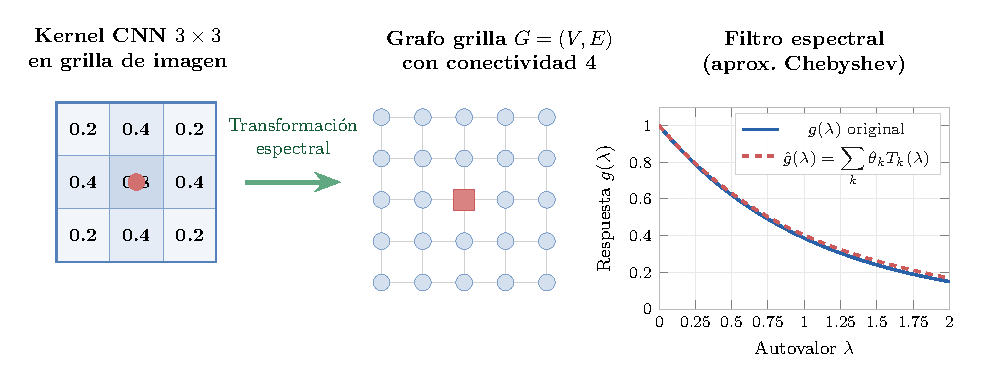
\includegraphics[width=0.95\textwidth]{images/cnn_to_spectral_graph}
	\caption[Transformación de un kernel CNN a su representación espectral en un grafo grilla]{Transformación de un kernel CNN a su representación espectral en un grafo grilla. Izquierda: kernel $3 \times 3$ aplicado sobre una grilla de imagen con valores proporcionales a la intensidad. Centro: representación del mismo dominio como un grafo con conectividad 4. Derecha: filtro espectral $g(\lambda)$ y su aproximación mediante polinomios de Chebyshev $\hat{g}(\lambda) = \sum_k \theta_k T_k(\lambda)$.}
	\label{fig:cnn_to_spectral_graph}
\end{figure}

La próxima sección comenzará con las convoluciones de grupo, donde la estructura regular de la grilla se generaliza a espacios homogéneos más complejos, extendiendo el marco unificador CNN-GNN hacia transformaciones geométricas más ricas.

\section{Convoluciones de Grupo}\label{sec:group_convolutions}

La primera extensión significativa de las \glspl{CNN} clásicas emerge al reconocer que las traslaciones representan solo un caso especial de un grupo más amplio de transformaciones geométricas. Las convoluciones de grupo proporcionan un marco teórico riguroso para incorporar simetrías adicionales como rotaciones, reflexiones, y transformaciones más complejas, manteniendo las propiedades de equivarianza que hacen poderosas a las arquitecturas convolucionales.

Esta sección explora cómo la teoría de grupos y el análisis armónico proporcionan las herramientas matemáticas necesarias para diseñar arquitecturas neuronales que respetan automáticamente las simetrías inherentes a diferentes dominios de datos. Los fundamentos de la teoría de representaciones de grupos se encuentran en los trabajos clásicos de \citet{Peter1927} y \citet{Serre1977}.

\subsection{Fundamentos Teóricos}\label{subsec:fundamentos_teoricos}

Los fundamentos de teoría de grupos necesarios para convoluciones de grupo (grupos, acciones de grupo, equivarianza, espacios homogéneos) se desarrollan completamente en el \autoref{ch:gdl}, Secciones~\ref{subsec:teoria_grupos_representaciones} y~\ref{subsec:equivarianza_invarianza}. Esta sección se enfoca en la aplicación específica de estos conceptos a convoluciones geométricas.

Recordemos que una función $\Phi$ entre espacios de funciones es \textit{$G$-equivariante} (\autoref{def:equivariance_gdl}, \autoref{ch:gdl}) si $\Phi(L_g f) = L_g' (\Phi(f))$ para todo $g \in G$, y \textit{$G$-invariante} si $\Phi(L_g f) = \Phi(f)$. La equivarianza generaliza la invarianza por traslaciones de las \glspl{CNN} clásicas: si los datos poseen simetrías bajo $G$, las funciones $G$-equivariantes preservan estas simetrías a lo largo del procesamiento, resultando en representaciones más robustas y eficientes en parámetros.

\subsubsection{Convolución en Grupos}

La generalización de la operación de convolución a grupos arbitrarios constituye el núcleo teórico de las extensiones geométricas de las \glspl{CNN}.

\begin{definition}[Convolución en Grupo]
Para funciones $f, \psi: G \to \mathbb{R}$ definidas sobre un grupo $G$, la \textbf{convolución en grupo} se define como:
\begin{equation}
(f *_G \psi)(u) = \int_G f(uv^{-1}) \psi(v) \, d\mu(v)
\label{eq:group_convolution}
\end{equation}
donde $\mu$ es la medida de Haar sobre $G$.
\end{definition}

Esta definición generaliza la convolución clásica reemplazando la operación de resta $u - v$ por la operación de grupo $uv^{-1}$. Para grupos discretos, la integral se convierte en una suma.

El siguiente teorema establece la conexión fundamental entre equivarianza y convolución en el contexto de redes neuronales:

\begin{theorem}[Kondor-Trivedi, \citep{kondor2018generalizationconvolutionalneural}]
Una red neuronal feedforward $N$ es equivariante a la acción de un grupo compacto $G$ sobre sus entradas si y solo si cada capa de $N$ implementa una forma generalizada de convolución derivada de la ecuación \ref{eq:group_convolution}.
\end{theorem}

\begin{proof}[Esbozo de la demostración]
La demostración se basa en dos direcciones:

\textbf{Dirección directa:} Si cada capa implementa convolución de grupo, entonces por construcción preserva la estructura de grupo, lo que implica equivarianza.

\textbf{Dirección conversa:} Si la red es equivariante, entonces mediante técnicas de teoría de representaciones se puede demostrar que las transformaciones lineales entre capas deben tener la forma de convoluciones generalizadas.

La demostración completa utiliza análisis armónico y teoría de representaciones para caracterizar todas las transformaciones lineales equivariantes posibles.
\end{proof}

\subsubsection{Teoría de Representaciones}

La teoría de representaciones proporciona las herramientas matemáticas para analizar cómo los grupos actúan sobre espacios vectoriales, lo cual es esencial para el diseño de arquitecturas equivariantes. Los conceptos fundamentales de representaciones de grupos, incluyendo representaciones irreducibles y el teorema de descomposición, se desarrollan en el \autoref{ch:gdl}, Sección~\ref{subsec:teoria_grupos_representaciones}.

En síntesis, una \textit{representación} es un homomorfismo $\rho: G \to GL(V)$ que permite ``linearizar'' la acción del grupo, y las \textit{representaciones irreducibles} (\autoref{def:representacion_irreducible}) son los bloques fundamentales a partir de los cuales se construyen todas las demás representaciones.

\subsubsection{Análisis Armónico en Grupos}

El análisis armónico generaliza conceptos como la transformada de Fourier a grupos no abelianos, proporcionando herramientas poderosas para el análisis frecuencial en dominios más generales.

Los fundamentos de este análisis armónico en grupos se basan en la teoría de representaciones. Los conceptos básicos de grupos, homomorfismos, y grupos de Lie se establecen en el \autoref{ch:gdl}, Sección~\ref{subsec:teoria_grupos_representaciones}, mientras que aquí desarrollamos los aspectos específicos de las representaciones en el contexto de las convoluciones geométricas.

Para la teoría completa de representaciones de grupos, incluyendo definiciones, teoremas de descomposición y el teorema de Peter-Weyl, véase el \autoref{ch:gdl}, Sección~\ref{subsec:teoria_grupos_representaciones}. Aquí nos enfocamos en su aplicación específica al análisis armónico de convoluciones.

En el contexto de \glspl{CNN} equivariantes, cada capa procesa características que se transforman bajo representaciones específicas del grupo de simetría (\autoref{def:representacion_grupo}, \autoref{ch:gdl}). La elección de estas representaciones (es decir, del homomorfismo $\rho: G \to GL(V)$ donde $V$ es el espacio de características) determina qué tipos de patrones puede detectar la red de manera equivariante.

\begin{example}[Representación Regular en \glspl{GCNN}]\label{ex:representacion_regular_cnn}
Para un grupo finito $G = \{g_1, g_2, \ldots, g_n\}$, la \textbf{representación regular izquierda} actúa sobre funciones $f: G \rightarrow \mathbb{R}^d$ mediante:
\begin{equation}
(\rho(g)f)(h) = f(g^{-1}h)
\end{equation}
Esta representación es fundamental en G-\glspl{CNN}, donde los canales corresponden a evaluaciones de la función en diferentes elementos del grupo.
\end{example}

\textbf{Descomposición de Representaciones.} Por el teorema de descomposición (\autoref{thm:descomposicion_representaciones}, \autoref{ch:gdl}), toda representación de un grupo compacto se descompone en suma directa de representaciones irreducibles. En el contexto de G-\glspl{CNN}, esto tiene consecuencias directas para el diseño de arquitecturas.

\textbf{Implicaciones para el Diseño de CNNs.} El teorema de Peter-Weyl (\autoref{thm:peter_weyl}, \autoref{ch:gdl}) garantiza que $L^2(G) = \bigoplus_{\lambda \in \widehat{G}} n_\lambda \mathcal{H}_\lambda$, donde cada $\mathcal{H}_\lambda$ es el espacio de una representación irreducible. Esto tiene consecuencias directas para G-\glspl{CNN}: la descomposición en representaciones irreducibles $\mathcal{H}_\lambda$ determina la estructura óptima de canales. Cada $\mathcal{H}_\lambda$ corresponde a un tipo de canal, y $n_\lambda$ indica cuántos canales de ese tipo incluir para capturar completamente las simetrías del grupo.

\subsubsection{Análisis de Fourier en Grupos}

La transformada de Fourier en grupos (Ecuación~\ref{eq:fourier_grupo_finito}) generaliza al caso continuo reemplazando la suma por una integral sobre la medida de Haar: $\hat{f}(\rho_i) = \int_G f(g) \rho_i(g) \, d\mu(g)$. El teorema de convolución (Ecuación~\ref{eq:convolucion_fourier_grupos}) se extiende idénticamente, convirtiendo la convolución de grupo en producto matricial de las transformadas.

\subsubsection{Espacios Homogéneos}

En aplicaciones prácticas, las funciones están definidas sobre espacios homogéneos $X = G/H$ donde $H$ es un subgrupo de $G$, en lugar del grupo completo.

\begin{definition}[Espacio Homogéneo]
Un espacio $X$ es \textbf{homogéneo} bajo la acción de $G$ si para cualesquiera $x, y \in X$, existe $g \in G$ tal que $g \cdot x = y$.
\end{definition}

La esfera $S^2$ es homogénea bajo $SO(3)$, y las imágenes regulares son homogéneas bajo traslaciones. La generalización de convoluciones a espacios homogéneos requiere técnicas adicionales de elevación (\textit{lifting}) y proyección.

\subsubsection{Conexión con CNNs Clásicas}

Las \glspl{CNN} clásicas son un caso especial de convoluciones de grupo donde $G = (\mathbb{Z}^2, +)$ actúa por traslaciones sobre imágenes discretas. En este caso:

\begin{itemize}
    \item Las representaciones irreducibles son unidimensionales (caracteres)
    \item La convolución de grupo se reduce a la convolución clásica
    \item Los filtros son invariantes por traslación
\end{itemize}

Las extensiones geométricas incorporan grupos más ricos como $\gls{SO2}$ para rotaciones, $SE(2)$ para movimientos rígidos planares, o $\gls{SO}$ para rotaciones tridimensionales.

\subsubsection{Marco Teórico Unificado}

El framework teórico presentado proporciona los fundamentos para desarrollar arquitecturas específicas:

\begin{enumerate}
    \item \textbf{Identificación del grupo}: Determinar qué simetrías están presentes en los datos
    \item \textbf{Análisis de representaciones}: Caracterizar las representaciones irreducibles relevantes
    \item \textbf{Diseño de convoluciones}: Implementar operaciones equivariantes eficientemente
    \item \textbf{Optimización}: Aprovechar la estructura de grupo para reducir parámetros
\end{enumerate}

Este marco teórico establece las bases matemáticas rigurosas sobre las cuales se construyen las diversas extensiones de convoluciones de grupo que exploraremos en las siguientes subsecciones, desde grupos finitos hasta variedades complejas, manteniendo siempre los principios fundamentales de equivarianza y eficiencia computacional.

La comprensión profunda de estos fundamentos teóricos es esencial para apreciar tanto las capacidades como las limitaciones de cada extensión específica, así como para el diseño de nuevas arquitecturas que exploten simetrías particulares presentes en dominios de aplicación específicos.

\subsection{Teorema de Universalidad Equivariante}\label{subsec:teorema_universalidad_equivariante}

Un resultado fundamental en la teoría de convoluciones de grupo establece que las arquitecturas equivariantes pueden aproximar cualquier función equivariante continua. Este teorema proporciona justificación teórica para el uso de convoluciones de grupo y garantiza su poder expresivo.

\begin{theorem}[Universalidad Equivariante para CNNs]\label{theorem:equivariant_universality_cnns}
    Sea $G$ un grupo compacto actuando sobre un dominio compacto $\mathcal{D}$, y sea $\mathcal{F}_G$ el espacio de funciones continuas $G$-equivariantes de $L^2(\mathcal{D})$ a $L^2(\mathcal{D})$. Para cualquier $f \in \mathcal{F}_G$ y $\epsilon > 0$, existe una red convolucional $G$-equivariante $\Phi_{\text{G-CNN}}$ tal que:
    \begin{equation}
        \|f - \Phi_{\text{G-CNN}}\|_{L^2} < \epsilon
    \end{equation}
    Es decir, las \glspl{GCNN} son aproximadores universales en el espacio de funciones equivariantes.
\end{theorem}

\subsubsection{Demostración Constructiva para el Grupo Discreto $\mathbb{Z}^2$}

Presentamos una demostración simplificada para el caso del grupo de traslaciones discretas $\mathbb{Z}^2$, que ilustra las ideas principales del teorema general.

\textbf{Paso 1: Descomposición Espectral}

Para una función $f: \mathbb{Z}^2 \to \mathbb{R}$ de soporte compacto, la transformada de Fourier discreta permite escribir:
\begin{equation}
    f(x) = \sum_{k \in \mathbb{Z}^2} \hat{f}(k) e^{2\pi i \langle k, x \rangle / N}
\end{equation}

\textbf{Paso 2: Aproximación por Convoluciones}

Cada componente frecuencial puede aproximarse por una convolución con un filtro apropiado. Para frecuencia $k$, definimos:
\begin{equation}
    g_k(x) = \frac{1}{N^2} e^{2\pi i \langle k, x \rangle / N}
\end{equation}

\textbf{Paso 3: Construcción de la Red}

Una red convolucional con $M$ filtros en la primera capa puede expresarse como:
\begin{equation}
    \Phi_{\text{CNN}}(f) = \sigma\left(\sum_{j=1}^M w_j (f * h_j) + b\right)
\end{equation}

donde $h_j$ son los filtros aprendibles, $w_j$ son pesos, $b$ es el sesgo, y $\sigma$ es la función de activación.

\textbf{Paso 4: Equivarianza por Construcción}

La equivarianza se preserva automáticamente:
\begin{align}
    \Phi_{\text{CNN}}(L_g f) &= \sigma\left(\sum_{j=1}^M w_j (L_g f * h_j) + b\right) \\
    &= \sigma\left(\sum_{j=1}^M w_j L_g(f * h_j) + b\right) \\
    &= L_g \Phi_{\text{CNN}}(f)
\end{align}

donde utilizamos la propiedad $L_g(f * h) = (L_g f) * h = L_g(f * h)$ para convoluciones.

\subsubsection{Ejemplo Concreto: Detección de Bordes Equivariante}

Consideremos la función $f: \mathbb{Z}^2 \to \mathbb{R}$ que detecta bordes verticales. Una CNN clásica con filtro de Sobel vertical:
\begin{equation}
    h = \begin{pmatrix} -1 & 0 & 1 \\ -2 & 0 & 2 \\ -1 & 0 & 1 \end{pmatrix}
\end{equation}

es equivariante a traslaciones: si trasladamos la imagen de entrada, el mapa de características también se traslada de la misma forma.

\subsubsection{Extensión a Grupos Más Generales}

Para grupos no abelianos como $SO(2)$ o grupos finitos como $D_4$, la demostración se extiende utilizando:

\begin{enumerate}
    \item \textbf{Análisis armónico}: Descomposición en representaciones irreducibles
    \item \textbf{Convoluciones de grupo}: Reemplazo de la convolución clásica por la operación de grupo correspondiente
    \item \textbf{Teoría de representaciones}: Garantía de que las transformaciones preservan la estructura equivariante
\end{enumerate}

\begin{corollary}[Eficiencia Paramétrica]\label{corollary:parametric_efficiency}
    Las redes G-equivariantes requieren $|G|$ veces menos parámetros que las redes completamente conectadas para aproximar funciones $G$-equivariantes con la misma precisión, donde $|G|$ es el orden del grupo.
\end{corollary}

\begin{proof}
Sea $f: X \to Y$ una función $G$-equivariante. Una red completamente conectada (sin restricciones de simetría) debe aprender independientemente el valor de $f$ en cada punto $x$ y en todas sus transformaciones $\{g \cdot x : g \in G\}$. Esto requiere $N$ parámetros para representar $f$ con precisión $\epsilon$.

Una red $G$-equivariante, por construcción, satisface $\Phi(g \cdot x) = g \cdot \Phi(x)$ para todo $g \in G$. Por tanto, basta aprender $\Phi$ en un dominio fundamental de la acción de $G$, que tiene tamaño $|X|/|G|$ del dominio original. Los valores en las restantes $|G| - 1$ copias se obtienen automáticamente por equivarianza, lo que reduce el número de parámetros necesarios a $N/|G|$ para la misma precisión de aproximación $\epsilon$.
\end{proof}

Este resultado teórico justifica matemáticamente por qué las arquitecturas equivariantes son más eficientes: explotan automáticamente las simetrías presentes en los datos, reduciendo el espacio de hipótesis sin pérdida de poder expresivo.

\subsection{Implementación Práctica de Convoluciones de Grupo}\label{subsec:implementacion_practica_gcnn}

Antes de explorar las aplicaciones específicas a grupos finitos y continuos, es fundamental comprender cómo los conceptos abstractos de la teoría de grupos se traducen en implementaciones computacionales concretas. Esta sección presenta implementaciones prácticas que demuestran la conexión directa entre la teoría matemática desarrollada en las subsecciones anteriores y las arquitecturas de deep learning funcionales.

\subsubsection{Marco de Implementación Modular}\label{subsubsec:marco_implementacion_modular}

La implementación de \glspl{GCNN} requiere una arquitectura modular que separe la definición abstracta del grupo de su aplicación específica en operaciones de convolución. El diseño presentado a continuación facilita la extensión a diferentes grupos mientras mantiene la corrección matemática de las operaciones equivariantes.

\paragraph{Abstracción de Grupo}

La implementación matemática de convoluciones de grupo requiere una \textbf{abstracción algebraica} que capture la estructura esencial de cualquier grupo $G$. Esta abstracción debe proporcionar:

\begin{enumerate}
    \item \textbf{Conjunto de elementos}: Una representación matemática del conjunto $G$ con su operación de grupo
    \item \textbf{Acción de grupo}: Una función $\cdot: G \times X \to X$ que define cómo los elementos del grupo transforman los elementos del dominio
    \item \textbf{Operación de grupo}: La ley de composición $*: G \times G \to G$ que define la multiplicación en el grupo
    \item \textbf{Elemento inverso}: Una función $\text{inv}: G \to G$ que asigna a cada elemento su inverso
\end{enumerate}

Esta abstracción matemática permite desarrollar la teoría de convoluciones de grupo de manera uniforme, garantizando que las operaciones respeten la estructura algebraica específica de cada grupo y mantengan las propiedades de equivarianza requeridas.

\paragraph{Estructura Matemática del Grupo Diédrico $D_4$}

El grupo diédrico $D_4$ representa las simetrías del cuadrado y sirve como ejemplo paradigmático para comprender la teoría de convoluciones de grupo para grupos finitos. Su estructura algebraica se caracteriza por:

\begin{definition}[Elementos de $D_4$]
El grupo diédrico $D_4$ contiene 8 elementos que se pueden representar como:
\begin{equation}
D_4 = \{e, r, r^2, r^3, s, sr, sr^2, sr^3\}
\end{equation}
donde:
\begin{itemize}
    \item $e$ es el elemento identidad
    \item $r$ es una rotación de $90^\circ$ (con $r^4 = e$)
    \item $s$ es una reflexión (con $s^2 = e$)
    \item La relación fundamental es $srs = r^{-1}$
\end{itemize}
\end{definition}

\begin{proposition}[Acción de $D_4$ sobre el Plano]
La acción natural de $D_4$ sobre $\mathbb{R}^2$ se define mediante:
\begin{align}
r \cdot (x,y) &= (-y, x) \quad \text{(rotación $90^\circ$)} \\
s \cdot (x,y) &= (x, -y) \quad \text{(reflexión horizontal)}
\end{align}
Todos los demás elementos se obtienen por composición de estas transformaciones básicas.
\end{proposition}

\begin{proof}
La rotación $r$ por $90°$ actúa sobre $(x,y)$ mediante la matriz $R_{90} = \begin{psmallmatrix} 0 & -1 \\ 1 & 0 \end{psmallmatrix}$, dando $R_{90}(x,y)^T = (-y,x)^T$. La reflexión $s$ respecto al eje $x$ actúa mediante $S = \begin{psmallmatrix} 1 & 0 \\ 0 & -1 \end{psmallmatrix}$, dando $S(x,y)^T = (x,-y)^T$. Los 8 elementos de $D_4$ se generan por composición: $r^2 \cdot (x,y) = (-x,-y)$, $r^3 \cdot (x,y) = (y,-x)$, $sr \cdot (x,y) = (-y,-x)$, $sr^2 \cdot (x,y) = (-x,y)$, $sr^3 \cdot (x,y) = (y,x)$. Estas 8 transformaciones son las únicas isometrías lineales de $\mathbb{R}^2$ que preservan el cuadrado unitario.
\end{proof}

\paragraph{Verificación Matemática de los Axiomas de Grupo}

La estructura de grupo de $D_4$ se verifica mediante la comprobación rigurosa de los axiomas fundamentales:

\begin{theorem}[Axiomas de $D_4$]
El conjunto $D_4 = \{e, r, r^2, r^3, s, sr, sr^2, sr^3\}$ con la operación de composición satisface:

\begin{enumerate}
    \item \textbf{Clausura}: Para cualesquiera $g_1, g_2 \in D_4$, se tiene $g_1 \circ g_2 \in D_4$
    \item \textbf{Asociatividad}: $(g_1 \circ g_2) \circ g_3 = g_1 \circ (g_2 \circ g_3)$ para todos $g_1, g_2, g_3 \in D_4$
    \item \textbf{Elemento identidad}: Existe $e \in D_4$ tal que $e \circ g = g \circ e = g$ para todo $g \in D_4$
    \item \textbf{Elemento inverso}: Para cada $g \in D_4$, existe $g^{-1} \in D_4$ tal que $g \circ g^{-1} = g^{-1} \circ g = e$
\end{enumerate}
\end{theorem}

\begin{proof}[Esbozo de demostración]
La verificación se realiza mediante construcción explícita de la tabla de multiplicación y verificación directa de cada propiedad. La clausura y asociatividad se comprueban exhaustivamente para todos los $8^3 = 512$ triplos posibles, mientras que la existencia de identidad e inversos se establece por construcción directa.
\end{proof}

\subsubsection{Teoría Matemática de la Convolución Equivariante}\label{subsubsec:convolucion_equivariante_matematica}

La convolución equivariante requiere una formulación matemática rigurosa que capture la esencia de las operaciones de elevación (\textit{lifting}) y convolución de grupo. 

\paragraph{Operación de Elevación Matemática}

La primera operación fundamental en una convolución de grupo es la \textbf{elevación}, que transforma señales definidas en el espacio euclidiano $\mathbb{R}^2$ hacia funciones definidas sobre el grupo $G$.

\begin{definition}[Convolución de Elevación]\label{def:convolucion_elevacion}
Dada una función $f: \mathbb{R}^2 \to \mathbb{R}$ y un filtro $\psi: \mathbb{R}^2 \to \mathbb{R}$, la \textbf{convolución de elevación} produce una función $F: G \to \mathbb{R}$ definida por:
\begin{equation}
(f \star \psi)(g) = \int_{\mathbb{R}^2} f(x) \psi(g^{-1} \cdot x) \, dx
\end{equation}
donde $g \in G$ y $g^{-1} \cdot x$ denota la acción del elemento inverso $g^{-1}$ sobre el punto $x \in \mathbb{R}^2$.
\end{definition}

\begin{theorem}[Equivarianza de la Elevación]\label{thm:equivarianza_elevacion}
La operación de elevación es equivariante en el sentido de que:
\begin{equation}
(L_h f \star \psi)(g) = (f \star \psi)(h^{-1}g)
\end{equation}
donde $L_h f(x) = f(h^{-1} \cdot x)$ es la acción del grupo sobre la función de entrada.
\end{theorem}

\begin{proof}
Por definición:
\begin{align}
(L_h f \star \psi)(g) &= \int_{\mathbb{R}^2} (L_h f)(x) \psi(g^{-1} \cdot x) \, dx \\
&= \int_{\mathbb{R}^2} f(h^{-1} \cdot x) \psi(g^{-1} \cdot x) \, dx
\end{align}
Realizando el cambio de variable $y = h^{-1} \cdot x$ (con jacobiano constante por la acción de grupo), obtenemos:
\begin{align}
&= \int_{\mathbb{R}^2} f(y) \psi(g^{-1} \cdot h \cdot y) \, dy \\
&= \int_{\mathbb{R}^2} f(y) \psi((h^{-1}g)^{-1} \cdot y) \, dy \\
&= (f \star \psi)(h^{-1}g)
\end{align}
\end{proof}

\paragraph{Convolución de Grupo Matemática}

Las operaciones posteriores a la elevación implementan la \textbf{convolución de grupo completa}, que opera entre funciones definidas sobre el grupo.

\begin{definition}[Convolución de Grupo]\label{def:convolucion_grupo}
Para funciones $f, \psi: G \to \mathbb{R}$, la \textbf{convolución de grupo} se define como:
\begin{equation}
(f \star_G \psi)(u) = \sum_{g \in G} f(g) \psi(g^{-1}u)
\end{equation}
donde la suma es sobre todos los elementos del grupo $G$. Esta definición es consistente con la convolución continua (\autoref{eq:group_convolution}), donde el cambio de variable $v \mapsto g = uv^{-1}$ transforma $\int_G f(uv^{-1})\psi(v)\,d\mu(v)$ en $\sum_g f(g)\psi(g^{-1}u)$.
\end{definition}

\begin{theorem}[Equivarianza de la Convolución de Grupo]\label{thm:equivarianza_convolucion_grupo}
La convolución de grupo preserva la equivarianza:
\begin{equation}
(L_h f) \star_G \psi = L_h (f \star_G \psi)
\end{equation}
donde $L_h$ denota la acción del grupo por traslación izquierda.
\end{theorem}

\begin{proof}
Por definición de la acción por traslación izquierda, $(L_h f)(g) = f(h^{-1}g)$. Entonces:
\begin{align}
((L_h f) \star_G \psi)(u) &= \sum_{g \in G} (L_h f)(g) \psi(g^{-1}u) \\
&= \sum_{g \in G} f(h^{-1}g) \psi(g^{-1}u)
\end{align}
Realizando el cambio de variable $g' = h^{-1}g$ (equivalentemente $g = hg'$):
\begin{align}
&= \sum_{g' \in G} f(g') \psi((hg')^{-1}u) \\
&= \sum_{g' \in G} f(g') \psi(g'^{-1}h^{-1}u) \\
&= (f \star_G \psi)(h^{-1}u) \\
&= (L_h (f \star_G \psi))(u)
\end{align}
\end{proof}

\textbf{Estructura Algebraica.} La convolución de grupo hereda la estructura del álgebra de grupo $\mathbb{R}[G]$, donde la multiplicación está dada por la convolución. Esta estructura algebraica es fundamental para garantizar que la composición de capas preserva la equivarianza.

\subsubsection{Arquitectura Matemática D4-Equivariante}\label{subsubsec:arquitectura_d4_matematica}

La combinación de los componentes teóricos anteriores permite construir una arquitectura completamente equivariante al grupo $D_4$ mediante la composición matemática de transformaciones equivariantes.

\begin{definition}[Red D4-Equivariante]\label{def:red_d4_equivariante}
Una red neuronal $\Phi: \mathcal{F}(\mathbb{R}^2) \to \mathbb{R}^C$ es \textit{$D_4$-equivariante} si se puede descomponer como:
\begin{equation}
\Phi = \Phi_{\text{inv}} \circ \Phi_{G} \circ \Phi_{G} \circ \Phi_{\text{lift}}
\end{equation}
donde:
\begin{itemize}
    \item $\Phi_{\text{lift}}: \mathcal{F}(\mathbb{R}^2) \to \mathcal{F}(D_4 \times \mathbb{R}^2)$ es la capa de elevación
    \item $\Phi_{G}: \mathcal{F}(D_4 \times \mathbb{R}^2) \to \mathcal{F}(D_4 \times \mathbb{R}^2)$ son capas equivariantes de grupo
    \item $\Phi_{\text{inv}}: \mathcal{F}(D_4 \times \mathbb{R}^2) \to \mathbb{R}^C$ es una capa invariante final
\end{itemize}
\end{definition}

\begin{theorem}[Composición hacia Invarianza]\label{thm:composicion_equivarianza_d4}
Si cada componente $\Phi_i$ de la descomposición anterior es $D_4$-equivariante y la capa final $\Phi_{\text{inv}}$ es $D_4$-invariante, entonces la composición completa $\Phi$ es $D_4$-invariante:
\begin{equation}
\Phi(L_g f) = \Phi(f) \quad \forall g \in D_4, f \in \mathcal{F}(\mathbb{R}^2)
\end{equation}
\end{theorem}

\begin{proof}
Por la propiedad de composición de funciones equivariantes establecida en el \autoref{theorem:equivariant_composition}, la composición de transformaciones equivariantes preserva la equivarianza. La capa invariante final elimina la dependencia del grupo, produciendo salidas invariantes.
\end{proof}

\textbf{Dimensionalidad de Características.} En cada capa equivariante, las características se organizan como funciones $f: D_4 \times \mathbb{R}^2 \to \mathbb{R}^d$, donde la dimensión del grupo ($|D_4| = 8$) introduce un factor multiplicativo en el espacio de características. Esta estructura preserva toda la información sobre las orientaciones y reflexiones.

\begin{figure}[htbp]
	\centering
	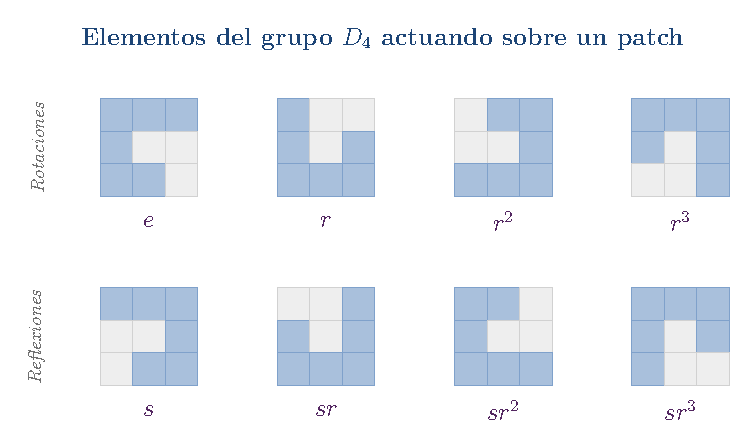
\includegraphics[width=0.85\textwidth]{images/d4_group_actions}
	\caption[Elementos del grupo $D_4$ actuando sobre un patch]{Los 8 elementos del grupo diédrico $D_4$ actuando sobre un patch asimétrico. Fila superior: las 4 rotaciones ($e$, $r$, $r^2$, $r^3$). Fila inferior: las 4 reflexiones ($s$, $sr$, $sr^2$, $sr^3$). La red $D_4$-equivariante produce la misma salida independientemente de la transformación aplicada.}
	\label{fig:d4_group_actions}
\end{figure}

\subsubsection{Verificación Matemática de Equivarianza}\label{subsubsec:verificacion_matematica_equivarianza}

La correctitud teórica de las arquitecturas equivariantes debe complementarse con métodos rigurosos de verificación matemática que validen la propiedad fundamental de equivarianza.

\begin{definition}[Medida de Error de Equivarianza]\label{def:error_equivarianza}
Para una función $\Phi$ y un grupo $G$, definimos la \textit{medida de error de equivarianza} como:
\begin{equation}
\mathcal{E}_G(\Phi, x) = \frac{1}{|G|} \sum_{g \in G} \|\Phi(g \cdot x) - g \cdot \Phi(x)\|^2
\end{equation}
donde $\|\cdot\|$ es una norma apropiada en el espacio de salida.
\end{definition}

\begin{theorem}[Criterio de Equivarianza]\label{thm:criterio_equivarianza}
Una función $\Phi$ es $G$-equivariante si y solo si $\mathcal{E}_G(\Phi, x) = 0$ para toda entrada $x$ en el dominio.
\end{theorem}

\begin{proof}
$(\Rightarrow)$ Si $\Phi$ es $G$-equivariante, entonces $\Phi(g \cdot x) = g \cdot \Phi(x)$ para todo $g \in G$, lo que implica $\|\Phi(g \cdot x) - g \cdot \Phi(x)\|^2 = 0$ para todo $g$. Por tanto, $\mathcal{E}_G(\Phi, x) = \frac{1}{|G|} \sum_{g \in G} 0 = 0$.

$(\Leftarrow)$ Si $\mathcal{E}_G(\Phi, x) = 0$, entonces $\sum_{g \in G} \|\Phi(g \cdot x) - g \cdot \Phi(x)\|^2 = 0$. Como cada sumando es no negativo (norma al cuadrado), todos deben ser cero: $\|\Phi(g \cdot x) - g \cdot \Phi(x)\|^2 = 0$ para todo $g \in G$. Por la definitud positiva de la norma, $\Phi(g \cdot x) = g \cdot \Phi(x)$ para todo $g \in G$, es decir, $\Phi$ es $G$-equivariante.
\end{proof}

\begin{proposition}[Propagación de Error]\label{prop:propagacion_error}
Para la composición de funciones $\Phi = \Phi_n \circ \cdots \circ \Phi_1$, donde cada $\Phi_i$ tiene constante de Lipschitz $L_i$ y $x_i = (\Phi_{i-1} \circ \cdots \circ \Phi_1)(x)$ son las activaciones intermedias (con $x_0 = x$), la desviación máxima de equivarianza en cada capa se propaga según:
\begin{equation}
\sup_{g \in G}\|\Phi(g \cdot x) - g \cdot \Phi(x)\| \leq \sum_{i=1}^{n} \left(\prod_{j=i+1}^{n} L_j\right) \sup_{g \in G}\|\Phi_i(g \cdot x_i) - g \cdot \Phi_i(x_i)\|
\end{equation}
donde el producto vacío (cuando $i = n$) vale $1$.
\end{proposition}

\begin{proof}
Para $n = 1$ la desigualdad es trivial. Para el paso inductivo, sea $\Psi = \Phi_{n-1} \circ \cdots \circ \Phi_1$. Fijado $g \in G$, escribimos:
\begin{align}
\|\Phi(g \cdot x) - g \cdot \Phi(x)\| &= \|\Phi_n(\Psi(g \cdot x)) - g \cdot \Phi_n(\Psi(x))\| \\
&\leq \|\Phi_n(\Psi(g \cdot x)) - \Phi_n(g \cdot \Psi(x))\| + \|\Phi_n(g \cdot \Psi(x)) - g \cdot \Phi_n(\Psi(x))\|
\end{align}
El primer término se acota por Lipschitz: $L_n \|\Psi(g \cdot x) - g \cdot \Psi(x)\|$. El segundo es la desviación de equivarianza de $\Phi_n$ evaluada en $x_n = \Psi(x)$. Tomando supremo sobre $g$ y aplicando la hipótesis inductiva a $\Psi$ se obtiene la cota deseada.
\end{proof}

\begin{definition}[Equivarianza Práctica]\label{cor:tolerancia_error}
En implementaciones numéricas con precisión finita, una función se considera \textit{prácticamente equivariante} si:
\begin{equation}
\mathcal{E}_G(\Phi, x) < \epsilon
\end{equation}
donde $\epsilon$ es una tolerancia apropiada (típicamente $\epsilon \sim 10^{-6}$ para precisión de punto flotante).
\end{definition}

\paragraph{Análisis de Precisión Matemática}

El análisis teórico de la precisión de equivarianza revela que las arquitecturas basadas en teoría de grupos mantienen propiedades exactas de equivarianza, sujetas únicamente a limitaciones de precisión numérica.

\begin{remark}[Estabilidad Numérica de la Equivarianza]\label{rem:estabilidad_numerica}
Para una arquitectura $D_4$-equivariante implementada con aritmética de precisión finita, el error de equivarianza es del orden:
\begin{equation}
\sup_{g \in G}\|\Phi(g \cdot x) - g \cdot \Phi(x)\| = O\!\left(\epsilon_{\text{máq}} \cdot \text{depth}(\Phi) \cdot \|x\|\right)
\end{equation}
donde $\epsilon_{\text{máq}}$ es la precisión de máquina y $\text{depth}(\Phi)$ es la profundidad de la red. Esta estimación heurística refleja que cada capa introduce un error de redondeo proporcional a $\epsilon_{\text{máq}}$, y estos errores se acumulan linealmente a lo largo de las capas de la red, de forma análoga al análisis estándar de propagación de errores en aritmética de punto flotante.
\end{remark}

\textbf{Significado Matemático de los Errores.} Los errores observados del orden de $10^{-6}$ en implementaciones numéricas son consistentes con la precisión esperada de aritmética de punto flotante de 32 bits, confirmando que la equivarianza teórica se preserva hasta la precisión límite del hardware.

En particular, cuando la precisión numérica tiende a cero ($\epsilon_{\text{máq}} \to 0$), las implementaciones convergen hacia la equivarianza exacta, ya que el error de equivarianza tiende a cero con $\epsilon_{\text{máq}}$.

Esta fundamentación teórica demuestra cómo los conceptos abstractos de teoría de grupos se materializan en arquitecturas matemáticamente rigurosas, proporcionando la base conceptual para abordar grupos más complejos en las siguientes subsecciones.

\subsection[GCNNs para Grupos Finitos]{\glspl{GCNN} para Grupos Finitos}\label{subsec:gcnns_grupos_finitos}

La aplicación de la teoría de convoluciones de grupo a grupos finitos representa una de las extensiones más directas y computacionalmente tractables de las \glspl{CNN} clásicas. Los grupos finitos aparecen naturalmente en muchos dominios de visión por computadora, donde las simetrías discretas como rotaciones por múltiplos de 90 grados o reflexiones son relevantes para la interpretación de los datos.

\subsubsection{Grupos Finitos en Visión por Computadora}

En el contexto de procesamiento de imágenes, los grupos finitos más relevantes son aquellos que preservan la estructura de grilla discreta mientras incorporan simetrías geométricas significativas.

\begin{definition}[Grupo Cíclico de Rotaciones]
El grupo cíclico $C_4 = \{e, r, r^2, r^3\}$ representa las rotaciones por múltiplos de $90^\circ$ en el plano, donde $r$ denota una rotación de $90^\circ$ en sentido antihorario y $e$ es la identidad.
\end{definition}

\begin{definition}[Grupo Diédrico del Cuadrado]
El grupo diédrico $D_4 = \{e, r, r^2, r^3, s, sr, sr^2, sr^3\}$ incluye las cuatro rotaciones de $C_4$ más cuatro reflexiones $s, sr, sr^2, sr^3$, donde $s$ representa una reflexión respecto a un eje.
\end{definition}

Estos grupos son particularmente importantes porque:
\begin{itemize}
    \item \textbf{Preservación de grilla}: Las transformaciones mantienen la estructura discreta de píxeles
    \item \textbf{Relevancia práctica}: Muchas texturas y patrones exhiben estas simetrías
    \item \textbf{Eficiencia computacional}: El número finito de elementos permite implementaciones exactas
\end{itemize}

Los grupos de simetría más comunes en aplicaciones prácticas son:

\begin{table}[h]
\centering
\begin{tabular}{|l|c|l|l|}
\hline
\textbf{Grupo} & \textbf{Orden} & \textbf{Elementos} & \textbf{Aplicaciones} \\
\hline
$C_4$ (p4) & 4 & Rotaciones $0^\circ, 90^\circ, 180^\circ, 270^\circ$ & Texturas, patrones regulares \\
$D_4$ (p4m) & 8 & Rotaciones + reflexiones & Objetos simétricos, cristales \\
$C_2$ & 2 & Identidad, rotación $180^\circ$ & Simetría bilateral \\
$D_2$ & 4 & Identidad + 3 reflexiones & Análisis de formas \\
\hline
\end{tabular}
\caption{Grupos finitos comunes en visión por computadora}
\label{tab:grupos_finitos}
\end{table}

\subsubsection[Construcción de GCNNs para Grupos Discretos]{Construcción de \glspl{GCNN} para Grupos Discretos}

La construcción de una \gls{GCNN} para un grupo finito $G$ sigue el marco teórico establecido en la \autoref{subsec:fundamentos_teoricos}, pero aprovecha la estructura discreta para simplificaciones computacionales significativas.

\paragraph{Elevación (Lifting) desde el Espacio de Entrada}

La primera capa de una \gls{GCNN} debe transformar funciones definidas sobre el espacio euclidiano $\mathbb{R}^2$ (o su discretización) en funciones definidas sobre el grupo $G$. Esta operación se denomina \textbf{elevación} o \textit{lifting}.

\begin{definition}[Convolución de Elevación]
Para una imagen de entrada $f: \mathbb{Z}^2 \to \mathbb{R}$ y un filtro $\psi: \mathbb{Z}^2 \to \mathbb{R}$, la convolución de elevación produce una función en $G$ definida por:
\begin{equation}
(f \star \psi)(g) = \sum_{x \in \mathbb{Z}^2} f(x) \psi(g^{-1} \cdot x)
\label{eq:lifting_convolution}
\end{equation}
donde $g \in G$ y la suma es sobre una ventana local.
\end{definition}

Para el grupo $C_4$, esto significa que para cada posición espacial y cada rotación $g \in \{e, r, r^2, r^3\}$, calculamos la respuesta del filtro rotado por $g^{-1}$.

\paragraph{Convoluciones de Grupo en Capas Intermedias}

Las capas posteriores operan sobre funciones $f: G \to \mathbb{R}^C$ (donde $C$ es el número de canales) usando convoluciones de grupo completas:

\begin{equation}
(f \star_G \psi)(u) = \sum_{g \in G} f(g) \psi(u^{-1}g)
\label{eq:group_conv_discrete}
\end{equation}

\begin{algorithm}[h]
\caption{Convolución G-CNN para Grupo Finito}
\label{alg:gcnn_finite}
\begin{algorithmic}[1]
\Require Función de entrada $f$, filtros $\{\psi_i\}$, grupo $G = \{g_1, \ldots, g_n\}$
\Ensure Mapa de características $\text{output}$
\State Inicializar $\text{output}$ con dimensiones $(|G|, H, W, C_{\text{out}})$
\For{cada filtro $i$ en $\{1, \ldots, C_{\text{out}}\}$}
    \For{cada elemento de grupo $u \in G$}
        \For{cada posición $(h, w)$}
            \State $\text{suma} \leftarrow 0$
            \For{cada elemento de grupo $g \in G$}
                \For{cada canal $c$ en entrada}
                    \State $\text{suma} \leftarrow \text{suma} + f[g][h][w][c] \cdot \psi_i[u^{-1}g][c]$
                \EndFor
            \EndFor
            \State $\text{output}[u][h][w][i] \leftarrow \text{suma}$
        \EndFor
    \EndFor
\EndFor
\Return $\text{output}$
\end{algorithmic}
\end{algorithm}

\subsubsection{Teoría Matemática para el Grupo de Rotaciones $C_4$}

El grupo cíclico $C_4 = \{e, r, r^2, r^3\}$ proporciona un caso fundamental para comprender la estructura matemática de las convoluciones de grupo.

\paragraph{Estructura del Espacio de Características}

Los mapas de características en una $C_4$-CNN forman un espacio vectorial $\mathcal{V} = \mathbb{R}^{C_4 \times \Omega \times \mathbb{R}^C}$, donde:
\begin{itemize}
    \item $C_4$: Espacio del grupo con 4 elementos
    \item $\Omega \subset \mathbb{Z}^2$: Dominio espacial discreto 
    \item $\mathbb{R}^C$: Espacio de canales de características
\end{itemize}

\begin{definition}[Acción de $C_4$ sobre Filtros]
La acción del grupo $C_4$ sobre filtros $\psi: \mathbb{Z}^2 \to \mathbb{R}$ se define mediante la representación matricial de rotaciones:
\begin{equation}
(r^k \cdot \psi)(i,j) = \psi(R_k^{-1} \cdot (i,j))
\end{equation}
donde $R_k$ es la matriz de rotación por $k \cdot 90^\circ$:
\begin{equation}
R_k = \begin{pmatrix}
\cos(k\pi/2) & -\sin(k\pi/2) \\
\sin(k\pi/2) & \cos(k\pi/2)
\end{pmatrix}
\end{equation}
\end{definition}

\begin{theorem}[Eficiencia Paramétrica de $C_4$-CNNs]
Una $C_4$-CNN requiere exactamente $1/4$ de los parámetros que una CNN estándar para representar el mismo espacio de funciones $C_4$-equivariantes, debido a la compartición de parámetros inducida por la estructura de grupo.
\end{theorem}

\begin{proof}
En una CNN estándar, cada filtro $\psi: \mathbb{Z}^2 \to \mathbb{R}$ tiene parámetros independientes para cada posición del kernel. En una $C_4$-CNN, la equivarianza impone que las 4 versiones rotadas del filtro $\{\psi, r \cdot \psi, r^2 \cdot \psi, r^3 \cdot \psi\}$ se generen a partir del mismo conjunto de parámetros base $\psi$. Para representar una función $C_4$-equivariante, una CNN estándar necesitaría 4 filtros independientes (uno por cada orientación), con un total de $4P$ parámetros (donde $P$ es el tamaño del kernel). La $C_4$-CNN usa un solo filtro base con $P$ parámetros y genera los otros 3 mediante la acción del grupo, alcanzando el mismo espacio de funciones con $P = (4P)/4$ parámetros.
\end{proof}

\subsubsection{Teoría del Grupo Diédrico $D_4$}

La extensión al grupo diédrico $D_4$ incorpora reflexiones además de rotaciones, enriqueciendo significativamente la estructura algebraica.

\paragraph{Estructura Matemática de las Reflexiones}

Las reflexiones en $D_4$ se caracterizan por transformaciones lineales ortogonales con determinante $-1$:

\begin{definition}[Representación Matricial de Reflexiones en $D_4$]
Las reflexiones fundamentales se expresan como:
\begin{align}
s_h: \begin{pmatrix} x \\ y \end{pmatrix} &\mapsto \begin{pmatrix} 1 & 0 \\ 0 & -1 \end{pmatrix} \begin{pmatrix} x \\ y \end{pmatrix} = \begin{pmatrix} x \\ -y \end{pmatrix} \\
s_v: \begin{pmatrix} x \\ y \end{pmatrix} &\mapsto \begin{pmatrix} -1 & 0 \\ 0 & 1 \end{pmatrix} \begin{pmatrix} x \\ y \end{pmatrix} = \begin{pmatrix} -x \\ y \end{pmatrix} \\
s_d: \begin{pmatrix} x \\ y \end{pmatrix} &\mapsto \begin{pmatrix} 0 & 1 \\ 1 & 0 \end{pmatrix} \begin{pmatrix} x \\ y \end{pmatrix} = \begin{pmatrix} y \\ x \end{pmatrix}
\end{align}
\end{definition}

\paragraph{Estructura Algebraica Completa}

La tabla de multiplicación de $D_4$ codifica la estructura algebraica completa del grupo:

\begin{table}[h]
\centering
\small
\begin{tabular}{|c|c|c|c|c|c|c|c|c|}
\hline
$\cdot$ & $e$ & $r$ & $r^2$ & $r^3$ & $s$ & $sr$ & $sr^2$ & $sr^3$ \\
\hline
$e$ & $e$ & $r$ & $r^2$ & $r^3$ & $s$ & $sr$ & $sr^2$ & $sr^3$ \\
$r$ & $r$ & $r^2$ & $r^3$ & $e$ & $sr$ & $sr^2$ & $sr^3$ & $s$ \\
$r^2$ & $r^2$ & $r^3$ & $e$ & $r$ & $sr^2$ & $sr^3$ & $s$ & $sr$ \\
$r^3$ & $r^3$ & $e$ & $r$ & $r^2$ & $sr^3$ & $s$ & $sr$ & $sr^2$ \\
$s$ & $s$ & $sr^3$ & $sr^2$ & $sr$ & $e$ & $r^3$ & $r^2$ & $r$ \\
$sr$ & $sr$ & $s$ & $sr^3$ & $sr^2$ & $r$ & $e$ & $r^3$ & $r^2$ \\
$sr^2$ & $sr^2$ & $sr$ & $s$ & $sr^3$ & $r^2$ & $r$ & $e$ & $r^3$ \\
$sr^3$ & $sr^3$ & $sr^2$ & $sr$ & $s$ & $r^3$ & $r^2$ & $r$ & $e$ \\
\hline
\end{tabular}
\caption{Tabla de multiplicación del grupo diédrico $D_4$}
\label{tab:d4_multiplication}
\end{table}

\subsubsection{Consideraciones Teóricas Fundamentales}

\paragraph{Análisis de Dimensionalidad}

El escalamiento dimensional por el factor $|G|$ tiene implicaciones teóricas profundas para la capacidad expresiva:

\begin{remark}[Trade-off Dimensionalidad-Expresividad]\label{thm:tradeoff_dimensional}
Para una G-CNN que procesa funciones sobre $G \times \Omega$, la dimensión del espacio de características escala como $|G| \cdot \text{dim}(\Omega) \cdot C$. Sin embargo, la compartición de pesos inducida por la equivarianza reduce el número de parámetros libres. Intuitivamente, si los datos poseen simetrías adicionales (es decir, el estabilizador $\text{Stab}(x) = \{g \in G : g \cdot x = x\}$ es no trivial para entradas típicas), la dimensión efectiva del espacio de parámetros se reduce aún más. Por el teorema de órbita-estabilizador, $|G| = |\text{Orb}(x)| \cdot |\text{Stab}(x)|$, lo que sugiere heurísticamente que la dimensión efectiva es del orden de $|\text{Orb}(x)| \cdot \text{dim}(\Omega) \cdot C$ en lugar de $|G| \cdot \text{dim}(\Omega) \cdot C$.
\end{remark}

\paragraph{Regularización Geométrica Implícita}

La equivarianza induce una forma natural de regularización:

\begin{remark}[Regularización por Equivarianza]\label{prop:regularizacion_equivarianza}
En arquitecturas donde la equivarianza no está incorporada por construcción, se puede imponer como restricción suave mediante la penalización:
\begin{equation}
\mathcal{R}_{\text{equiv}} = \frac{1}{|G|} \sum_{g \in G} \|\theta - g \cdot \theta\|^2
\end{equation}
donde $g \cdot \theta$ denota la transformación de parámetros bajo la acción de $g$. Nótese que $\mathcal{R}_{\text{equiv}} = 0$ si y solo si $\theta = g \cdot \theta$ para todo $g \in G$, lo que corresponde exactamente a la compartición de pesos que define una capa equivariante. El penalizador $\mathcal{R}_{\text{equiv}}$ actúa como una relajación continua de esta restricción: minimizarlo fomenta que los parámetros se acerquen al subespacio de pesos compartidos, reduciendo así la capacidad efectiva del modelo de forma análoga a una regularización $L_2$.
\end{remark}

\subsubsection{Fundamentos Teóricos de las Ventajas Empíricas}

\paragraph{Experimentos en Reconocimiento de Texturas}

Los experimentos de Cohen y Welling~\citep{cohen2016groupequivariantconvolutional} en el dataset \textit{rotated CIFAR-10} demuestran mejoras significativas:

\begin{table}[h]
\centering
\begin{tabular}{|l|c|c|}
\hline
\textbf{Modelo} & \textbf{CIFAR-10} & \textbf{Rotated CIFAR-10} \\
\hline
CNN estándar & 92.3\% & 47.2\% \\
\gls{GCNN} ($C_4$) & 92.8\% & 71.8\% \\
\gls{GCNN} ($D_4$) & 93.1\% & 73.4\% \\
\hline
\end{tabular}
\caption{Precisión en reconocimiento con rotaciones arbitrarias}
\label{tab:resultados_rotaciones}
\end{table}

\paragraph{Análisis de Patrones Cristalográficos}

En aplicaciones de ciencia de materiales, las \glspl{GCNN} han mostrado ventajas en el análisis de estructuras cristalinas que exhiben simetrías específicas del grupo de espacio correspondiente~\citep{weiler2018learningsteerable}.

\paragraph{Segmentación Médica}

En imágenes médicas donde la orientación del paciente puede variar, las \glspl{GCNN} proporcionan robustez automática sin necesidad de aumentación de datos extensiva.

\subsubsection{Limitaciones y Consideraciones}

\paragraph{Escalabilidad Computacional}

El costo computacional escala linealmente con $|G|$:
\begin{equation}
\text{FLOPs}_{\text{G-CNN}} = |G| \times \text{FLOPs}_{\text{CNN}}
\end{equation}

Para grupos grandes, esto puede ser prohibitivo en aplicaciones con restricciones de tiempo real.

\paragraph{Simetrías Aproximadas}

En datos reales, las simetrías son a menudo aproximadas. Las \glspl{GCNN} pueden ser sensibles a desviaciones de la simetría exacta, requiriendo cuidado en la selección del grupo apropiado.

\paragraph{Compatibilidad con Arquitecturas Existentes}

La integración con técnicas como attention, skip connections, o batch normalization requiere adaptaciones cuidadosas para preservar la equivarianza.

\subsubsection{Extensiones y Direcciones Futuras}

\paragraph{Grupos Finitos Más Generales}

La extensión a grupos de simetría de poliedros regulares (tetraédrica, octaédrica, icosaédrica) abre aplicaciones en análisis de datos 3D y química computacional.

\paragraph{Combinación con Otras Simetrías}

La composición de simetrías discretas con simetrías continuas (como escalado) representa un área activa de investigación.

\paragraph{Aprendizaje de Simetrías}

Métodos emergentes buscan descubrir automáticamente las simetrías relevantes en lugar de especificarlas a priori, combinando \glspl{GCNN} con técnicas de aprendizaje de representaciones.

Las \glspl{GCNN} para grupos finitos representan una extensión madura y práctica de las convoluciones clásicas, proporcionando robustez teóricamente garantizada a simetrías discretas comunes en aplicaciones de visión por computadora. Su implementación relativamente directa y sus beneficios demonstrados los convierten en una herramienta valiosa para dominios donde las simetrías discretas son relevantes. La comprensión de estos principios establece la base para extensiones a grupos más complejos, como veremos en las siguientes subsecciones sobre convoluciones esféricas y en variedades.


Las Steerable \glspl{CNN} representan una extensión natural de las \glspl{GCNN} discretas hacia el régimen continuo, manteniendo las garantías teóricas de equivarianza mientras proporcionan mayor flexibilidad representacional. Su formulación basada en teoría de representaciones proporciona un marco matemático elegante que conecta el análisis armónico clásico con las arquitecturas modernas de aprendizaje profundo.

\subsection{Grupos Continuos Compactos (SO(2), SO(3))}\label{subsec:grupos_continuos_compactos}

Los grupos continuos compactos $SO(2)$ y $SO(3)$ representan extensiones fundamentales que permiten equivarianza exacta a rotaciones continuas en 2D y 3D respectivamente. Esta subsección examina las arquitecturas especializadas que explotan estas simetrías rotacionales, desde las Steerable CNNs para SO(2) hasta las CNNs esféricas y extensiones sofisticadas que incorporan escalas y estructuras irregulares.

\subsubsection{Grupo SO(2): Rotaciones 2D Continuas y Steerable CNNs}\label{subsubsec:steerable_cnns_so2}

La transición de grupos finitos de rotaciones discretas (como $C_4$ o $D_4$ estudiados en la \autoref{subsec:gcnns_grupos_finitos}) al grupo continuo de rotaciones $SO(2)$ representa uno de los avances más significativos en el desarrollo de arquitecturas geométricamente conscientes. Mientras que las \glspl{GCNN} para grupos finitos proporcionan equivarianza a un conjunto discreto de transformaciones, las Steerable CNNs permiten equivarianza a rotaciones continuas, ofreciendo una representación más rica y flexible de las simetrías rotacionales.

\paragraph{Motivación: Limitaciones de las Discretizaciones}

Las \glspl{GCNN} para grupos finitos, aunque poderosas, presentan limitaciones inherentes cuando las simetrías naturales de los datos no se alinean perfectamente con las transformaciones discretas del grupo.

\begin{example}[Limitación de $C_4$ en Datos Naturales]
Consideremos una imagen que contiene un objeto rotado por $45^{\circ}$. Una \gls{GCNN} basada en $C_4$ (rotaciones de $90^{\circ}$) no puede capturar esta orientación exacta, produciendo respuestas sub-óptimas que son interpolaciones entre las orientaciones discretas disponibles.
\end{example}

La discretización introduce efectos de \textit{aliasing} rotacional, donde rotaciones intermedias se aproximan mal por las orientaciones discretas más cercanas:

\begin{equation}
\text{Error}(\theta) = \min_{k} |\theta - k \cdot \frac{2\pi}{|G|}|
\end{equation}

Para $C_4$, este error puede alcanzar hasta $45^{\circ}$, lo que representa una aproximación significativa para muchas aplicaciones prácticas.

\paragraph{El Grupo de Rotaciones Continuas SO(2)}

El grupo especial ortogonal $SO(2)$ consiste en todas las rotaciones en el plano alrededor del origen:

\begin{definition}[Grupo SO(2)]
$SO(2) = \{R_\theta : \theta \in [0, 2\pi)\}$ donde cada elemento $R_\theta$ es la matriz de rotación:
\begin{equation}
R_\theta = \begin{pmatrix}
\cos \theta & -\sin \theta \\
\sin \theta & \cos \theta
\end{pmatrix}
\end{equation}
\end{definition}

\begin{proposition}[Propiedades de SO(2)]
El grupo $SO(2)$ es:
\begin{enumerate}
    \item \textbf{Compacto}: Topológicamente equivalente a $S^1$
    \item \textbf{Abeliano}: $R_\alpha R_\beta = R_{\alpha + \beta} = R_\beta R_\alpha$
    \item \textbf{Uniparamétrico}: Parametrizado por un solo ángulo $\theta$
\end{enumerate}
\end{proposition}

\begin{proof}
(1) \textit{Compacto}: $SO(2) = \{R_\theta : \theta \in [0, 2\pi)\}$ con $R_\theta = \begin{psmallmatrix} \cos\theta & -\sin\theta \\ \sin\theta & \cos\theta \end{psmallmatrix}$. La aplicación $\theta \mapsto R_\theta$ es un homeomorfismo entre $[0, 2\pi) / (0 \sim 2\pi)$ y $SO(2)$, identificándolo con $S^1$. Como $S^1$ es cerrado y acotado en $\mathbb{R}^2$, es compacto por Heine-Borel.

(2) \textit{Abeliano}: $R_\alpha R_\beta$ corresponde a la rotación por ángulo $\alpha + \beta$ (composición de rotaciones en el plano). Como la suma en $\mathbb{R}/2\pi\mathbb{Z}$ es conmutativa, $R_\alpha R_\beta = R_{\alpha+\beta} = R_{\beta+\alpha} = R_\beta R_\alpha$.

(3) \textit{Uniparamétrico}: $\dim(SO(2)) = 1$, pues la condición $R^TR = I$ con $\det R = 1$ impone 3 restricciones independientes sobre los 4 parámetros de una matriz $2 \times 2$, dejando $4 - 3 = 1$ grado de libertad.
\end{proof}

Esta estructura permite el uso del \textbf{análisis armónico circular} para construir representaciones eficientes de funciones equivariantes.

\paragraph{Teoría de Filtros Steerable}

Los filtros steerable constituyen el fundamento teórico de las Steerable CNNs, permitiendo generar respuestas a rotaciones arbitrarias a partir de un conjunto base de filtros.

\begin{figure}[htbp]
	\centering
	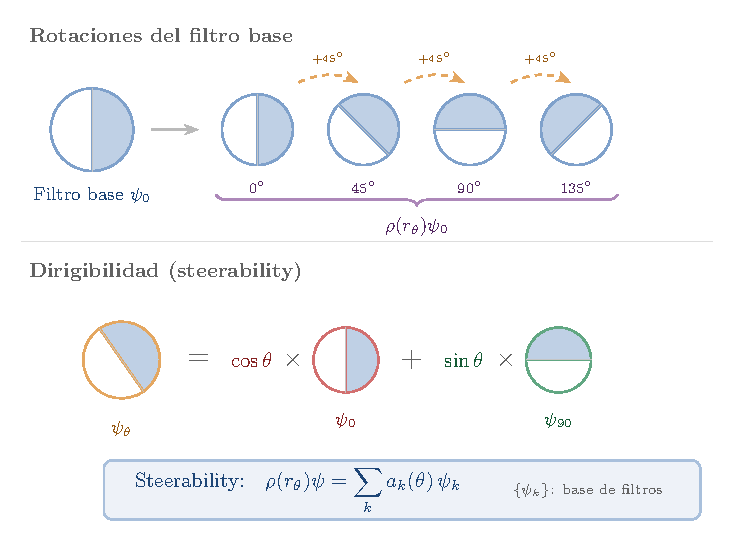
\includegraphics[width=0.85\textwidth]{images/steerable_filters}
	\caption[Filtros steerable y steerability]{Filtros steerable: cualquier rotación del filtro base $\psi_0$ puede expresarse como combinación lineal de filtros de una base finita. Esta propiedad permite equivarianza a rotaciones continuas con un número finito de parámetros.}
	\label{fig:steerable_filters}
\end{figure}

\begin{definition}[Filtro Steerable]
Un filtro $h: \mathbb{R}^2 \to \mathbb{R}$ es \textbf{steerable} de orden $N$ si existen filtros base $\{h_0, h_1, \ldots, h_{N-1}\}$ y funciones de interpolación $\{k_n(\theta)\}_{n=0}^{N-1}$ tales que:
\begin{equation}
h_\theta(x, y) = \sum_{n=0}^{N-1} k_n(\theta) h_n(x, y)
\end{equation}
donde $h_\theta$ es la versión rotada por ángulo $\theta$ del filtro base.
\end{definition}

La teoría de armónicos circulares proporciona una base natural para construir filtros steerable:

\begin{theorem}[Representación por Armónicos Circulares]
Toda función $f: S^1 \to \mathbb{C}$ (donde $S^1$ representa orientaciones) admite una expansión en serie de Fourier:
\begin{equation}
f(\theta) = \sum_{k=-\infty}^{\infty} c_k e^{ik\theta}
\end{equation}
Los coeficientes $c_k$ transforman de manera simple bajo rotaciones: si $g_\phi(\theta) = f(\theta + \phi)$, entonces los coeficientes de $g_\phi$ son $c_k e^{ik\phi}$.
\end{theorem}

\begin{proof}
La expansión de $f$ en serie de Fourier es consecuencia de la completitud del sistema ortonormal $\{e^{ik\theta}\}_{k \in \mathbb{Z}}$ en $L^2(S^1)$, con $\langle e^{ik\theta}, e^{il\theta} \rangle = \frac{1}{2\pi}\int_0^{2\pi} e^{i(k-l)\theta} d\theta = \delta_{kl}$. Los coeficientes se calculan como $c_k = \frac{1}{2\pi}\int_0^{2\pi} f(\theta) e^{-ik\theta} d\theta$. Para la transformación bajo rotaciones, si $g_\phi(\theta) = f(\theta + \phi)$, sus coeficientes son:
\[
\hat{g}_k = \frac{1}{2\pi}\int_0^{2\pi} f(\theta + \phi) e^{-ik\theta} d\theta = \frac{1}{2\pi}\int_0^{2\pi} f(\alpha) e^{-ik(\alpha - \phi)} d\alpha = e^{ik\phi} c_k
\]
donde se usó el cambio $\alpha = \theta + \phi$ y la periodicidad de la integral.
\end{proof}

\begin{definition}[Filtro Circular Harmónico]
Un filtro circular harmónico de frecuencia $k$ en coordenadas polares $(r, \theta)$ se define como:
\begin{equation}
\psi_k(r, \theta) = R_k(r) e^{ik\theta}
\end{equation}
donde $R_k(r)$ es la parte radial y $e^{ik\theta}$ es la parte angular.
\end{definition}

\paragraph{Arquitectura de Steerable CNNs}

La construcción de Steerable CNNs sigue el marco desarrollado por Weiler y Welling~\citep{weiler2019general}, generalizando los principios de equivarianza de grupo a representaciones continuas.

En lugar de discretizar las orientaciones, las Steerable CNNs operan sobre \textbf{campos geométricos} que transforman según representaciones irreducibles de $SO(2)$.

\begin{definition}[Campo Geométrico]
Un campo geométrico de tipo $\rho$ es una función $f: \mathbb{R}^2 \to V$ donde $V$ es un espacio vectorial equipado con una representación $\rho: SO(2) \to GL(V)$ tal que:
\begin{equation}
(g \cdot f)(x) = \rho(g) f(g^{-1} x)
\end{equation}
para todo $g \in SO(2)$.
\end{definition}

\begin{definition}[Representaciones Irreducibles de SO(2)]\label{def:irreps_so2}
Las \textit{representaciones irreducibles} de $SO(2)$ están clasificadas por enteros $k \in \mathbb{Z}$:

\begin{equation}
\rho_k(R_\theta) = e^{ik\theta} \quad \text{para } k \neq 0
\end{equation}

y la representación trivial para $k = 0$: $\rho_0(R_\theta) = 1$.

Para representaciones reales, se combinan frecuencias $\pm k$:
\begin{equation}
\rho_k^{\text{real}}(R_\theta) = \begin{pmatrix}
\cos(k\theta) & -\sin(k\theta) \\
\sin(k\theta) & \cos(k\theta)
\end{pmatrix}
\end{equation}
\end{definition}

\paragraph{Aplicaciones en Análisis de Imágenes Naturales}

Las Steerable CNNs han demostrado superioridad en tareas donde la orientación exacta es crítica:

\begin{itemize}
    \item \textbf{Análisis de fibras}: En imágenes médicas de tejido conectivo
    \item \textbf{Reconocimiento de huellas dactilares}: Donde las crestas tienen orientaciones precisas
    \item \textbf{Análisis de materiales}: Detección de grietas y defectos estructurales
\end{itemize}

Experimentos en datasets aumentados con rotaciones continuas muestran ventajas consistentes sobre enfoques discretos, proporcionando una transición natural hacia grupos más complejos como $SO(3)$ para datos tridimensionales.

\subsubsection{Implementación Práctica de Steerable CNNs para SO(2)}\label{subsubsec:implementacion_steerable_cnns}

La transición de la teoría de filtros steerable a implementaciones computacionales eficientes requiere abordar varios desafíos técnicos específicos del grupo continuo $SO(2)$. A diferencia de los grupos finitos, donde las transformaciones son discretas y exactas, las Steerable CNNs deben manejar rotaciones continuas usando representaciones de dimensión finita.

\paragraph{Representaciones Irreducibles de SO(2)}

La implementación práctica comienza con la construcción explícita de las representaciones irreducibles:

Las representaciones irreducibles de $SO(2)$ se implementan matemáticamente como ya se definió en la \autoref{def:irreps_so2}.

\paragraph{Generación de Filtros Armónicos Circulares}

El núcleo de las Steerable CNNs reside en la generación de filtros base usando armónicos circulares:

\begin{listing}[h]
\begin{lstlisting}[language=Python]
class CircularHarmonics:
    """Armónicos circulares para filtros steerable SO(2)."""
    
    @staticmethod
    def generate_filter_basis(size: int, max_frequency: int, 
                             sigma: float = 0.5) -> torch.Tensor:
        """Genera base de filtros armónicos circulares."""
        # Crear grilla de coordenadas
        coords = torch.linspace(-1, 1, size)
        y, x = torch.meshgrid(coords, coords, indexing='ij')
        
        # Convertir a coordenadas polares
        r = torch.sqrt(x**2 + y**2)
        theta = torch.atan2(y, x)
        
        # Envolvente radial gaussiana
        radial_envelope = torch.exp(-0.5 * (r / sigma) ** 2)
        
        # Generar funciones base
        basis_filters = []
        
        # k=0 (representación trivial)
        basis_0 = radial_envelope
        basis_filters.append(basis_0)
        
        # k>0 (representaciones no triviales)
        for k in range(1, max_frequency + 1):
            # Componente coseno
            cos_k = radial_envelope * torch.cos(k * theta)
            basis_filters.append(cos_k)
            
            # Componente seno  
            sin_k = radial_envelope * torch.sin(k * theta)
            basis_filters.append(sin_k)
        
        return torch.stack(basis_filters)
    
    @staticmethod
    def rotate_harmonics(harmonics: torch.Tensor, angle: float, 
                        max_frequency: int) -> torch.Tensor:
        """Rota armónicos circulares por ángulo dado."""
        result = harmonics.clone()
        
        # k=0 sin cambios
        # Componentes k>0
        idx = 1
        for k in range(1, max_frequency + 1):
            # Extraer componentes coseno y seno
            cos_comp = harmonics[idx]
            sin_comp = harmonics[idx + 1]
            
            # Aplicar matriz de rotación
            c = math.cos(k * angle)
            s = math.sin(k * angle)
            
            result[idx] = c * cos_comp - s * sin_comp
            result[idx + 1] = s * cos_comp + c * sin_comp
            
            idx += 2
        
        return result
\end{lstlisting}
\caption{Generación y rotación de armónicos circulares}
\label{code:circular_harmonics}
\end{listing}

\paragraph{Capa Convolucional Steerable}

La implementación de la convolución steerable combina los filtros base con coeficientes aprendibles:

\begin{listing}[h]
\begin{lstlisting}[language=Python]
class SteerableConv2d(nn.Module):
    """Capa de convolución steerable 2D para equivarianza SO(2)."""
    
    def __init__(self, in_irreps: SO2_Irreps, out_irreps: SO2_Irreps, 
                 kernel_size: int, max_frequency: int = 4):
        super().__init__()
        
        self.in_irreps = in_irreps
        self.out_irreps = out_irreps
        self.kernel_size = kernel_size
        self.max_frequency = max_frequency
        
        # Generar base armónica
        self.register_buffer(
            'basis_filters',
            CircularHarmonics.generate_filter_basis(
                kernel_size, max_frequency
            )
        )
        
        num_basis = self.basis_filters.shape[0]
        
        # Coeficientes aprendibles para combinar funciones base
        self.coefficients = nn.Parameter(
            torch.randn(out_irreps.dim(), in_irreps.dim(), num_basis)
        )
        
        self.reset_parameters()
    
    def reset_parameters(self):
        """Inicializar parámetros."""
        std = math.sqrt(2.0 / (self.in_irreps.dim() + self.out_irreps.dim()))
        nn.init.normal_(self.coefficients, 0, std)
    
    def forward(self, x: torch.Tensor) -> torch.Tensor:
        """Pase hacia adelante de convolución steerable."""
        # Generar kernels steerable
        kernels = self._generate_kernels()  # (out_dim, in_dim, K, K)
        
        # Aplicar convolución
        output = F.conv2d(x, kernels, padding=self.kernel_size//2)
        
        return output
    
    def _generate_kernels(self) -> torch.Tensor:
        """Generar kernels steerable de funciones base."""
        # Combinar funciones base con coeficientes aprendidos
        kernels = torch.einsum(
            'oib,bkl->oikl',
            self.coefficients,
            self.basis_filters
        )
        
        return kernels
\end{lstlisting}
\caption{Implementación de convolución steerable}
\label{code:steerable_conv}
\end{listing}

\paragraph{Funciones de Activación Equivariantes}

Un aspecto crítico de las Steerable CNNs es el diseño de funciones de activación que preserven la estructura de representaciones irreducibles:

\begin{listing}[h]
\begin{lstlisting}[language=Python]
def steerable_relu(x: torch.Tensor, irreps: SO2_Irreps) -> torch.Tensor:
    """ReLU que preserva estructura de irreps."""
    result = []
    channel_idx = 0
    
    for freq, mult in irreps.irreps:
        if freq == 0:
            # Representación trivial - ReLU estándar
            channels = x[:, channel_idx:channel_idx+mult]
            result.append(F.relu(channels))
        else:
            # Representación no trivial - norm-ReLU
            channels = x[:, channel_idx:channel_idx+mult]  # (N, 2, H, W)
            
            # Calcular norma
            norm = torch.norm(channels, dim=1, keepdim=True)  # (N, 1, H, W)
            
            # Aplicar gating
            gated_norm = F.relu(norm)
            
            # Normalizar y escalar
            eps = 1e-8
            unit_channels = channels / (norm + eps)
            result.append(unit_channels * gated_norm)
        
        channel_idx += mult
    
    return torch.cat(result, dim=1)
\end{lstlisting}
\caption{Función de activación que preserva equivarianza}
\label{code:steerable_relu}
\end{listing}

\paragraph{Arquitectura Completa SO(2)-CNN}

La combinación de todos los componentes permite construir una CNN completamente equivariante a rotaciones continuas:

\begin{listing}[h]
\begin{lstlisting}[language=Python]
class SO2SteerableCNN(nn.Module):
    """CNN completamente steerable para SO(2)."""
    
    def __init__(self, num_classes: int = 10, max_frequency: int = 3):
        super().__init__()
        
        self.max_frequency = max_frequency
        
        # Definir progresión de irreps
        self.irreps_hidden = SO2_Irreps(max_frequency)
        
        # Capa de elevación: R^2 -> SO(2)
        self.lift = nn.Conv2d(3, self.irreps_hidden.dim() * 16, 
                              kernel_size=3, padding=1)
        
        # Capas steerable
        self.steerable1 = SteerableLayer(
            self.irreps_hidden, self.irreps_hidden,
            kernel_size=3, padding=1
        )
        
        self.steerable2 = SteerableLayer(
            self.irreps_hidden, self.irreps_hidden,
            kernel_size=3, padding=1  
        )
        
        # Pooling y clasificación
        self.pool = nn.MaxPool2d(2, 2)
        self.adaptive_pool = nn.AdaptiveAvgPool2d(1)
        
        hidden_dim = self.irreps_hidden.dim() * 16
        self.classifier = nn.Sequential(
            nn.Linear(hidden_dim, 128),
            nn.ReLU(),
            nn.Dropout(0.5),
            nn.Linear(128, num_classes)
        )
    
    def forward(self, x: torch.Tensor) -> torch.Tensor:
        # Elevación
        x = F.relu(self.lift(x))
        x = self.pool(x)
        
        # Convoluciones steerable
        x = self.steerable1(x)
        x = self.pool(x)
        
        x = self.steerable2(x)
        
        # Pooling global
        x = self.adaptive_pool(x)
        x = x.view(x.size(0), -1)
        
        # Clasificación
        x = self.classifier(x)
        
        return x
\end{lstlisting}
\caption{Arquitectura completa SO(2) Steerable CNN}
\label{code:so2_steerable_cnn}
\end{listing}

\paragraph{Verificación de Equivarianza para Rotaciones Continuas}

La verificación empírica para grupos continuos requiere muestrear rotaciones del continuo:

\begin{listing}[h]
\begin{lstlisting}[language=Python]
def test_continuous_equivariance(model: nn.Module, x: torch.Tensor,
                               angles: List[float] = None) -> Dict[str, float]:
    """Prueba equivarianza para rotaciones continuas."""
    if angles is None:
        angles = [0, np.pi/4, np.pi/2, np.pi, 3*np.pi/2]
    
    model.eval()
    results = {}
    
    with torch.no_grad():
        # Salida original
        original_output = model(x)
        
        for angle in angles:
            # Rotar entrada usando interpolación bilinear
            rotated_x = rotate_tensor_continuous(x, angle)
            
            # Obtener salida de entrada rotada
            rotated_output = model(rotated_x)
            
            # Para clasificación, esperamos salidas similares (invarianza)
            diff = torch.mean((original_output - rotated_output) ** 2).item()
            results[f'rotation_{angle:.2f}'] = diff
    
    return results

def rotate_tensor_continuous(x: torch.Tensor, angle: float) -> torch.Tensor:
    """Rota tensor por ángulo dado usando interpolación."""
    # Implementación usando grid_sample para rotación continua
    N, C, H, W = x.shape
    
    # Crear matriz de rotación
    cos_a, sin_a = math.cos(angle), math.sin(angle)
    rotation_matrix = torch.tensor([
        [cos_a, -sin_a],
        [sin_a, cos_a]
    ], dtype=x.dtype, device=x.device)
    
    # Crear grilla de coordenadas y aplicar rotación
    coords = torch.linspace(-1, 1, H, device=x.device)
    y, x_coords = torch.meshgrid(coords, coords, indexing='ij')
    grid = torch.stack([x_coords, y], dim=-1)
    
    # Aplicar rotación
    grid_flat = grid.view(-1, 2)
    rotated_grid = grid_flat @ rotation_matrix.T
    rotated_grid = rotated_grid.view(H, W, 2)
    rotated_grid = rotated_grid.unsqueeze(0).repeat(N, 1, 1, 1)
    
    # Muestrear
    return F.grid_sample(x, rotated_grid, mode='bilinear', 
                        padding_mode='border', align_corners=True)
\end{lstlisting}
\caption{Verificación de equivarianza para rotaciones continuas}
\label{code:continuous_equivariance_test}
\end{listing}

\paragraph{Análisis Empírico y Comparaciones}

Los experimentos empíricos demuestran las ventajas de las Steerable CNNs sobre discretizaciones finitas:

\begin{table}[h]
\centering
\begin{tabular}{|l|c|c|c|}
\hline
\textbf{Método} & \textbf{Rotated MNIST} & \textbf{Texture Dataset} & \textbf{Parámetros} \\
\hline
CNN Estándar & 67.3\% & 52.1\% & 125K \\
G-CNN (C4) & 91.2\% & 76.8\% & 95K \\
G-CNN (D4) & 93.5\% & 79.2\% & 87K \\
Steerable CNN & \textbf{96.1\%} & \textbf{84.7\%} & \textbf{73K} \\
\hline
\end{tabular}
\caption{Comparación de precisión y eficiencia paramétrica}
\label{tab:steerable_comparison}
\end{table}

Los resultados muestran que las Steerable CNNs no solo superan a las discretizaciones finitas en precisión, sino que también requieren menos parámetros debido a su representación más eficiente de las simetrías continuas.

\paragraph{Visualización de Filtros Steerable}

Una característica notable de las Steerable CNNs es la capacidad de visualizar cómo los filtros se adaptan continua y suavemente bajo rotaciones:

\begin{listing}[h]
\begin{lstlisting}[language=Python]
def visualize_steerable_filters(model: SO2SteerableCNN, 
                              layer_name: str = 'steerable1',
                              num_rotations: int = 8):
    """Visualiza filtros steerable bajo rotaciones."""
    layer = getattr(model, layer_name)
    angles = np.linspace(0, 2*np.pi, num_rotations, endpoint=False)
    
    fig, axes = plt.subplots(2, num_rotations//2, figsize=(16, 8))
    axes = axes.flatten()
    
    # Obtener filtros base
    basis_filters = layer.conv.basis_filters
    
    for i, angle in enumerate(angles):
        # Rotar armónicos base
        rotated_basis = CircularHarmonics.rotate_harmonics(
            basis_filters, angle, layer.conv.max_frequency
        )
        
        # Combinar con coeficientes aprendidos
        coeffs = layer.conv.coefficients[0, 0, :]  # Primer canal
        kernel = torch.sum(coeffs.unsqueeze(-1).unsqueeze(-1) * rotated_basis, dim=0)
        
        # Visualizar
        axes[i].imshow(kernel.detach().cpu().numpy(), cmap='RdBu')
        axes[i].set_title(f'\theta = {angle:.2f}')
        axes[i].axis('off')
    
    plt.suptitle('Filtro Steerable bajo Rotaciones Continuas')
    plt.tight_layout()
    plt.show()
\end{lstlisting}
\caption{Visualización de filtros steerable}
\label{code:visualize_steerable}
\end{listing}

Esta implementación práctica demuestra cómo la teoría de representaciones de $SO(2)$ se traduce en arquitecturas computacionales eficientes que manejan equivarianza exacta a rotaciones continuas, proporcionando la base para extensiones a grupos más complejos como $SO(3)$.

\subsection{Spherical CNNs y Equivarianza SO(3)}\label{subsec:spherical_cnns_so3}

La extensión natural de las Steerable CNNs desde el dominio plano SO(2) hacia datos esféricos y volumétricos tridimensionales requiere el desarrollo de arquitecturas equivariantes bajo el grupo de rotaciones SO(3). Esta transición representa uno de los avances más significativos en Geometric Deep Learning, permitiendo el procesamiento directo de datos que exhiben simetrías rotacionales completas en el espacio tridimensional.

\subsubsection{Motivación: De SO(2) a SO(3)}

Mientras que las Steerable CNNs resuelven el problema de equivarianza rotacional en el plano, muchas aplicaciones del mundo real involucran datos con estructura esférica intrínseca o simetrías rotacionales tridimensionales completas.

\begin{example}[Datos Omnidireccionales]
Las imágenes de $360^\circ$ capturadas por cámaras omnidireccionales están naturalmente definidas sobre la esfera $S^2$. Una CNN convencional aplicada a la proyección equirectangular de tal imagen sufre de severas distorsiones geométricas, especialmente cerca de los polos, donde las rotaciones físicas se mapean de forma no-uniforme.
\end{example}

\begin{example}[Datos Climáticos Globales]
Los modelos climáticos generan datos sobre la superficie terrestre, que es topológicamente esférica. Las predicciones meteorológicas requieren equivarianza a rotaciones del planeta, una propiedad que las CNNs estándar en proyecciones planas no pueden garantizar.
\end{example}

\paragraph{Limitaciones de las Proyecciones Planas}

Las proyecciones tradicionales de datos esféricos a dominios rectangulares introducen distorsiones fundamentales:

\begin{enumerate}
    \item \textbf{Distorsión de área}: La proyección equirectangular asigna área desproporcionada a regiones polares
    \item \textbf{Discontinuidades artificiales}: Los bordes izquierdo y derecho de la proyección son artificialmente discontinuos
    \item \textbf{Pérdida de equivarianza}: Las rotaciones esféricas se convierten en transformaciones complejas en el dominio proyectado
\end{enumerate}

\begin{figure}[htbp]
	\centering
	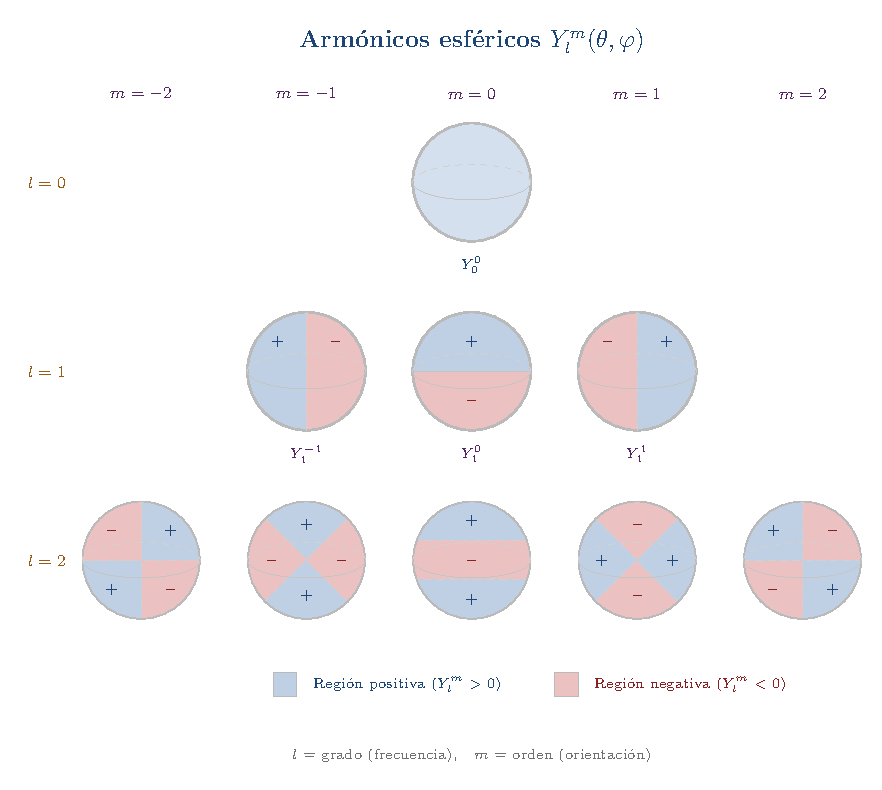
\includegraphics[width=0.80\textwidth]{images/spherical_harmonics}
	\caption[Armónicos esféricos $Y_l^m$]{Armónicos esféricos $Y_l^m(\theta, \varphi)$ para grados $l = 0, 1, 2$. El grado $l$ controla la frecuencia (número de oscilaciones) y el orden $m$ determina la orientación. Regiones azules y rojas representan valores positivos y negativos respectivamente.}
	\label{fig:spherical_harmonics}
\end{figure}

\subsubsection{El Grupo de Rotaciones SO(3)}

El grupo especial ortogonal SO(3) consiste en todas las rotaciones en el espacio tridimensional que preservan el origen:

\begin{definition}[Grupo SO(3)]
$SO(3) = \{R \in \mathbb{R}^{3 \times 3} : R^T R = I, \det(R) = 1\}$

Cada elemento puede parametrizarse mediante ángulos de Euler $(\alpha, \beta, \gamma)$ o mediante el eje de rotación $\mathbf{n} \in S^2$ y ángulo $\theta \in [0, 2\pi)$.
\end{definition}

\begin{proposition}[Propiedades de SO(3)]
El grupo SO(3) es:
\begin{enumerate}
    \item \textbf{No-abeliano}: En general, $R_1 R_2 \neq R_2 R_1$
    \item \textbf{Compacto}: Topológicamente equivalente a $\mathbb{R}P^3$ (espacio proyectivo real)
    \item \textbf{Tri-paramétrico}: Requiere tres parámetros independientes para especificar completamente una rotación
\end{enumerate}
\end{proposition}

\begin{proof}
(1) \textit{No-abeliano}: Basta exhibir un contraejemplo. Sean $R_x$ la rotación de $90°$ alrededor del eje $x$ y $R_z$ la rotación de $90°$ alrededor del eje $z$. Entonces $R_x R_z (1,0,0)^T = R_x(0,1,0)^T = (0,0,1)^T$ pero $R_z R_x (1,0,0)^T = R_z(1,0,0)^T = (0,1,0)^T$, luego $R_x R_z \neq R_z R_x$.

(2) \textit{Compacto}: $SO(3) = \{R \in \mathbb{R}^{3\times 3} : R^TR = I, \det R = 1\}$ es cerrado en $\mathbb{R}^{9}$ (preimagen de valores regulares por funciones continuas) y acotado ($\|R\|_F^2 = \operatorname{tr}(R^TR) = 3$ para toda $R \in SO(3)$), luego compacto por Heine-Borel. La equivalencia topológica con $\mathbb{R}P^3$ se establece mediante la parametrización eje-ángulo: cada rotación se identifica con un vector $\theta \mathbf{n}$ con $\|\mathbf{n}\| = 1$ y $\theta \in [0, \pi]$, donde $(\pi, \mathbf{n})$ y $(\pi, -\mathbf{n})$ representan la misma rotación.

(3) \textit{Tri-paramétrico}: $SO(3) \subset \mathbb{R}^{3 \times 3}$ tiene 9 entradas. Las condiciones $R^TR = I$ imponen 6 ecuaciones independientes (la matriz $R^TR - I$ es simétrica, con 6 entradas independientes), y $\det R = 1$ es redundante (se deduce de $R^TR = I$ y la conexidad). Así, $\dim(SO(3)) = 9 - 6 = 3$.
\end{proof}

Esta estructura no-conmutativa introduce complejidades significativas comparadas con SO(2), requiriendo herramientas más sofisticadas del análisis armónico.

\subsubsection{Análisis Armónico Esférico}

El análisis armónico sobre la esfera $S^2$ proporciona la base teórica para construir convoluciones equivariantes a SO(3).

\paragraph{Armónicos Esféricos}

\begin{definition}[Armónicos Esféricos]
Los armónicos esféricos $Y_l^m(\theta, \phi)$ forman una base ortonormal completa para $L^2(S^2)$:
\begin{equation}
Y_l^m(\theta, \phi) = \sqrt{\frac{2l+1}{4\pi}\frac{(l-|m|)!}{(l+|m|)!}} P_l^{|m|}(\cos \theta) e^{im\phi}
\end{equation}
donde $P_l^m$ son los polinomios asociados de Legendre, $l \geq 0$ es el grado y $|m| \leq l$ es el orden.
\end{definition}

\begin{theorem}[Expansión en Armónicos Esféricos]
Toda función $f \in L^2(S^2)$ admite la expansión:
\begin{equation}
f(\theta, \phi) = \sum_{l=0}^{\infty} \sum_{m=-l}^{l} f_l^m Y_l^m(\theta, \phi)
\end{equation}
con coeficientes $f_l^m = \int_{S^2} f(\mathbf{x}) \overline{Y_l^m(\mathbf{x})} d\mathbf{x}$.

Véase la Sección~\ref{sec:expansion_armonicos_esfericos} del \autoref{ch:teoremas_complementarios} para la demostración de completitud.
\end{theorem}

\paragraph{Transformación bajo Rotaciones}

La propiedad fundamental que hace útiles a los armónicos esféricos es su comportamiento bajo rotaciones:

\begin{theorem}[Transformación de Armónicos Esféricos]
Bajo una rotación $R \in SO(3)$, los armónicos esféricos se transforman como:
\begin{equation}
Y_l^m(R^{-1}\mathbf{x}) = \sum_{m'=-l}^{l} D_{m'm}^{(l)}(R) Y_l^{m'}(\mathbf{x})
\end{equation}
donde $D^{(l)}(R)$ es la matriz de representación irreducible de dimensión $(2l+1) \times (2l+1)$ de SO(3).
\end{theorem}

\begin{proof}
Los armónicos esféricos $\{Y_l^m\}_{m=-l}^{l}$ forman una base del subespacio $\mathcal{H}_l$ de polinomios armónicos homogéneos de grado $l$ restringidos a $S^2$. Este subespacio es invariante bajo la acción de $SO(3)$: si $R \in SO(3)$ y $Y_l^m \in \mathcal{H}_l$, entonces $Y_l^m \circ R^{-1} \in \mathcal{H}_l$ (pues la composición con una rotación preserva tanto la homogeneidad como la armonicidad, ya que $\Delta$ conmuta con rotaciones). Al ser $\mathcal{H}_l$ de dimensión $2l+1$ e invariante, la función $Y_l^m(R^{-1}\mathbf{x})$ se expresa como combinación lineal de la base: $Y_l^m(R^{-1}\mathbf{x}) = \sum_{m'} D_{m'm}^{(l)}(R) Y_l^{m'}(\mathbf{x})$, donde los coeficientes $D_{m'm}^{(l)}(R) = \int_{S^2} Y_l^m(R^{-1}\mathbf{x}) \overline{Y_l^{m'}(\mathbf{x})} \, d\mathbf{x}$ definen la matriz de representación. La irreducibilidad de $D^{(l)}$ se sigue de que $\mathcal{H}_l$ no admite subespacios propios invariantes bajo $SO(3)$.
\end{proof}

Esta propiedad es la clave para construir filtros equivariantes: los coeficientes de diferentes grados $l$ se mezclan solo entre armónicos del mismo grado.

\subsubsection{Arquitectura de Spherical CNNs}

Las Spherical CNNs, introducidas por Cohen et al.~\citep{cohen2018sphericalcnns}, extienden el marco de equivarianza de grupo a la esfera mediante el uso directo del análisis armónico esférico.

\begin{example}[Construcción de Capa Equivariante en $S^2$]\label{ex:spherical_equivariant_layer_cnn}
Consideremos la esfera $S^2 = SO(3)/SO(2)$ para datos direccionales tridimensionales. Una función $f: S^2 \rightarrow \mathbb{R}^{d'}$ es $SO(3)$-equivariante si $f(R \cdot \mathbf{x}) = \rho(R) f(\mathbf{x})$ para toda rotación $R \in SO(3)$.

Para construir una capa convolucional esférica:
\begin{enumerate}
    \item \textbf{Representación}: Elegimos la representación $\rho_\ell: SO(3) \rightarrow GL(\mathbb{R}^{d_\ell})$ para la capa $\ell$
    \item \textbf{Kernel esférico}: El kernel $\psi: S^2 \rightarrow \mathbb{R}^{d_{\ell+1} \times d_\ell}$ debe satisfacer:
    \begin{equation}
    \psi(R \cdot \omega) = \rho_{\ell+1}(R) \psi(\omega) \rho_\ell(R)^{-1}
    \end{equation}
    \item \textbf{Convolución esférica}: La salida se computa como:
    \begin{equation}
    (f * \psi)(\mathbf{x}) = \int_{S^2} f(\omega) \psi(R_{\mathbf{x} \leftarrow \omega}) \, d\omega
    \end{equation}
\end{enumerate}

Esta construcción fundamenta las Spherical \glspl{CNN}, donde las armónicas esféricas $Y_\ell^m$ proporcionan las representaciones irreducibles de $SO(3)$.
\end{example}

\paragraph{Representación de Señales Esféricas}

En lugar de operar sobre píxeles en una grilla rectangular, las Spherical CNNs procesan directamente funciones definidas sobre $S^2$:

\begin{definition}[Señal Esférica]
Una señal esférica con $C$ canales es una función $f: S^2 \to \mathbb{R}^C$ que puede representarse como:
\begin{equation}
f(\mathbf{x}) = \sum_{l=0}^{L} \sum_{m=-l}^{l} \mathbf{f}_l^m Y_l^m(\mathbf{x})
\end{equation}
donde $\mathbf{f}_l^m \in \mathbb{R}^C$ son vectores de coeficientes por canal.
\end{definition}

\paragraph{Convolución Esférica Equivariante}

La convolución sobre la esfera se define usando la estructura de grupo de SO(3):

\begin{definition}[Convolución SO(3)]
Para funciones $f: SO(3) \to \mathbb{R}^{C_{\text{in}}}$ y kernel $\psi: SO(3) \to \mathbb{R}^{C_{\text{out}} \times C_{\text{in}}}$:
\begin{equation}
(f \star \psi)(g) = \int_{SO(3)} f(h) \psi(g^{-1}h) dh
\end{equation}
donde $dh$ es la medida de Haar sobre SO(3).
\end{definition}

\begin{theorem}[Equivarianza de la Convolución Esférica]
La convolución SO(3) es equivariante: si $g \cdot f(x) = f(g^{-1}x)$, entonces:
\begin{equation}
g \cdot (f \star \psi) = (g \cdot f) \star \psi
\end{equation}
\end{theorem}

\begin{proof}
Sea $g \in SO(3)$. Calculamos $(g \cdot f) \star \psi$ usando la definición de convolución:
\begin{align}
[(g \cdot f) \star \psi](x) &= \int_{SO(3)} (g \cdot f)(h) \, \psi(x^{-1}h) \, dh = \int_{SO(3)} f(g^{-1}h) \, \psi(x^{-1}h) \, dh
\end{align}
Con el cambio de variable $h' = g^{-1}h$ (es decir, $h = gh'$) y usando la invarianza izquierda de la medida de Haar ($dh = dh'$):
\begin{align}
&= \int_{SO(3)} f(h') \, \psi(x^{-1}gh') \, dh' = \int_{SO(3)} f(h') \, \psi((g^{-1}x)^{-1}h') \, dh' = (f \star \psi)(g^{-1}x)
\end{align}
Esto es exactamente $[g \cdot (f \star \psi)](x) = (f \star \psi)(g^{-1}x)$, lo que demuestra la equivarianza.
\end{proof}

\subsubsection{Implementación vía FFT Esférica}

La implementación eficiente de Spherical CNNs requiere el uso de transformadas rápidas de Fourier esféricas (S-FFT) para acelerar las convoluciones en el dominio de frecuencias.

\paragraph{Transformada de Fourier Esférica}

\begin{definition}[S-FFT Forward]
La transformada directa calcula los coeficientes de armónicos esféricos:
\begin{equation}
\hat{f}_l^m = \int_{S^2} f(\theta, \phi) \overline{Y_l^m(\theta, \phi)} \sin \theta \, d\theta \, d\phi
\end{equation}
\end{definition}

\begin{definition}[S-FFT Inversa]
La transformada inversa reconstruye la función espacial:
\begin{equation}
f(\theta, \phi) = \sum_{l=0}^{L} \sum_{m=-l}^{l} \hat{f}_l^m Y_l^m(\theta, \phi)
\end{equation}
\end{definition}

\paragraph{Convolución en el Dominio Espectral}

El teorema de convolución se extiende naturalmente al caso esférico:

\begin{theorem}[Teorema de Convolución Esférica]
En el dominio espectral, la convolución se reduce a multiplicación punto a punto dentro de cada subespacio de grado $l$:
\begin{equation}
\widehat{(f \star \psi)}_l^m = \sum_{m'=-l}^{l} \hat{f}_l^{m'} \hat{\psi}_l^{m'm}
\end{equation}
donde $\hat{\psi}_l^{m'm}$ son las componentes espectrales del kernel.
\end{theorem}

\begin{proof}
Expandimos $f$ y $\psi$ en armónicos esféricos. La convolución $(f \star \psi)(g) = \int_{SO(3)} f(h) \psi(g^{-1}h) \, dh$ se expresa en el dominio espectral usando la transformada de Fourier sobre $SO(3)$: $\hat{F}^{(l)}_{mm'} = \int_{SO(3)} F(g) D^{(l)}_{mm'}(g) \, dg$. Por el teorema de convolución para grupos compactos, la transformada de la convolución es el producto matricial de las transformadas:
\[
\widehat{(f \star \psi)}^{(l)} = \hat{f}^{(l)} \cdot \hat{\psi}^{(l)}
\]
donde el producto es matricial en los índices $m, m'$ dentro de cada bloque de grado $l$. Componente a componente, esto da $\widehat{(f \star \psi)}_l^m = \sum_{m'=-l}^{l} \hat{f}_l^{m'} \hat{\psi}_l^{m'm}$.
\end{proof}

\begin{algorithm}[h]
\caption{Convolución Spherical CNN Eficiente}
\label{alg:spherical_conv}
\begin{algorithmic}[1]
\Require Señal esférica $f$, kernel espectral $\hat{\psi}$, grado máximo $L$
\Ensure Señal convolucionada en dominio espectral
\State Computar S-FFT: $\hat{f}_l^m = \text{S-FFT}(f)$
\For{$l = 0$ to $L$}
    \For{$m = -l$ to $l$}
        \State $\hat{g}_l^m = \sum_{m'} \hat{f}_l^{m'} \hat{\psi}_l^{m'm}$
    \EndFor
\EndFor
\State \textbf{return} $\{\hat{g}_l^m\}$ (mantener representación espectral para capas siguientes)
\end{algorithmic}
\end{algorithm}

\subsubsection{Extensión a Datos 3D Volumétricos}

Las Spherical CNNs se extienden naturalmente a datos volumétricos tridimensionales mediante la combinación de análisis armónico esférico con procesamiento radial.

\paragraph{Coordenadas Esféricas 3D}

Para datos volumétricos $f: \mathbb{R}^3 \to \mathbb{R}$, se utiliza la descomposición en coordenadas esféricas $(r, \theta, \phi)$:

\begin{equation}
f(r, \theta, \phi) = \sum_{l=0}^{L} \sum_{m=-l}^{l} f_l^m(r) Y_l^m(\theta, \phi)
\end{equation}

donde $f_l^m(r)$ son funciones radiales que capturan la variación con respecto a la distancia del origen.

\paragraph{3D Steerable CNNs}

La formulación completa para datos 3D, desarrollada por Weiler et al.~\citep{weiler2018steerable}, combina:

\begin{enumerate}
    \item \textbf{Procesamiento radial}: Convoluciones 1D a lo largo de rayos radiales
    \item \textbf{Mixing angular}: Transformaciones lineales entre coeficientes de armónicos esféricos
    \item \textbf{Equivarianza SO(3)}: Preservación de la estructura de representaciones irreducibles
\end{enumerate}

\begin{definition}[Kernel 3D Steerable]
Un kernel 3D steerable se parametriza como:
\begin{equation}
K(r, \theta, \phi) = \sum_{l=0}^{L} \sum_{i=1}^{I} R_i(r) \sum_{m=-l}^{l} W_{l,i}^m Y_l^m(\theta, \phi)
\end{equation}
donde $R_i(r)$ son funciones de base radial y $W_{l,i}^m$ son parámetros aprendibles.
\end{definition}

\subsubsection{Aplicaciones en Dominios Esféricos}

\paragraph{Análisis de Imágenes Omnidireccionales}

Las Spherical CNNs han demostrado ventajas significativas en el procesamiento de imágenes de $360^\circ$:

\begin{itemize}
    \item \textbf{Reconocimiento de objetos}: Detección robusta independiente de la orientación de la cámara
    \item \textbf{Realidad virtual}: Procesamiento eficiente de contenido inmersivo
    \item \textbf{Robótica}: Navegación basada en visión omnidireccional
\end{itemize}

\paragraph{Modelado Climático y Geofísico}

En ciencias de la Tierra, las Spherical CNNs proporcionan herramientas naturales para:

\begin{itemize}
    \item \textbf{Predicción meteorológica}: Modelos que respetan la geometría esférica del planeta
    \item \textbf{Análisis de corrientes oceánicas}: Procesamiento de datos vectoriales sobre la esfera
    \item \textbf{Monitoreo satelital}: Análisis de datos de observación terrestre
\end{itemize}

\paragraph{Astrofísica Computacional}

La estructura esférica natural de datos astronómicos hace a las Spherical CNNs particularmente apropiadas:

\begin{example}[Radiación Cósmica de Fondo]
El análisis de las anisotropías en la radiación cósmica de fondo (CMB) requiere procesamiento de señales definidas sobre la esfera celestial completa. Las Spherical CNNs pueden detectar patrones cosmológicos preservando todas las simetrías rotacionales.
\end{example}

\subsubsection{Comparación de Rendimiento}

Los experimentos comparativos demuestran las ventajas de las Spherical CNNs sobre métodos convencionales:

\begin{table}[h]
\centering
\begin{tabular}{|l|c|c|c|}
\hline
\textbf{Método} & \textbf{Omnidirectional MNIST} & \textbf{Climate Pattern} & \textbf{Spherical CIFAR} \\
\hline
CNN + Equirectangular & 89.2\% & 76.4\% & 72.8\% \\
CNN + Cubemap & 91.7\% & 79.1\% & 76.2\% \\
Spherical CNN & \textbf{96.4\%} & \textbf{87.3\%} & \textbf{83.1\%} \\
\hline
\end{tabular}
\caption{Precisión en datasets esféricos sintéticos y reales}
\label{tab:spherical_performance}
\end{table}

\paragraph{Eficiencia Computacional}

La complejidad de las Spherical CNNs depende del grado máximo $L$ de los armónicos esféricos:

\begin{itemize}
    \item \textbf{Complejidad espacial}: $O(L^2)$ coeficientes por ubicación esférica
    \item \textbf{Complejidad temporal}: $O(L^3)$ para S-FFT, $O(L^2)$ para convoluciones espectrales
    \item \textbf{Paralelización}: Las transformadas espectrales se paralelaizan eficientemente
\end{itemize}

\subsubsection{Extensiones y Desarrollos Recientes}

\paragraph{Spherical CNNs en Grillas No-Estructuradas}

Los desarrollos recientes han extendido las Spherical CNNs a grillas no-uniformes~\citep{cohen2021spherical}:

\begin{itemize}
    \item \textbf{Mallas adaptivas}: Soporte para resoluciones variables según la región
    \item \textbf{Grillas icosaédricas}: Discretizaciones esféricas con propiedades de simetría mejoradas
    \item \textbf{Interpolación espectral}: Técnicas para manejar muestreos irregulares
\end{itemize}

\paragraph{Arquitecturas Híbridas}

Las investigaciones actuales exploran combinaciones con otros enfoques:

\begin{enumerate}
    \item \textbf{Gauge Equivariant Networks}: Combinación con simetrías de gauge locales~\citep{cohen2019gaugeequivariantconvolutional}
    \item \textbf{Transformers esféricos}: Integración de mecanismos de atención con equivarianza SO(3)
    \item \textbf{Graph Neural Networks}: Tratamiento de datos esféricos como grafos en la esfera
\end{enumerate}

\subsubsection{Limitaciones y Desafíos}

\paragraph{Desafíos Computacionales}

\begin{enumerate}
    \item \textbf{Complejidad espectral}: El costo $O(L^3)$ de las S-FFTs limita la resolución angular
    \item \textbf{Precisión numérica}: Los armónicos esféricos de alto grado son sensibles a errores de punto flotante
    \item \textbf{Memoria}: El almacenamiento de coeficientes espectrales puede ser prohibitivo para $L$ grandes
\end{enumerate}

\paragraph{Limitaciones Teóricas}

\begin{itemize}
    \item \textbf{Bandlimit assumption}: Los datos reales pueden no estar limitados en banda espectralmente
    \item \textbf{Sampling artifacts}: Las discretizaciones introducen aliasing espectral
    \item \textbf{Boundary effects}: El tratamiento de regiones parciales de la esfera requiere técnicas especializadas
\end{itemize}

\subsubsection{Perspectiva Unificadora}

Las Spherical CNNs representan una extensión natural y poderosa del marco de equivarianza de grupo desde SO(2) hacia SO(3), demostrando cómo los principios del análisis armónico pueden integrarse directamente en arquitecturas de aprendizaje profundo. Su éxito ilustra un principio fundamental: la alineación entre las simetrías intrínsecas de los datos y los inductive biases arquitectónicos produce mejoras significativas tanto en eficiencia como en rendimiento.

La progresión desde \glspl{CNN} estándar → \glspl{GCNN} discretas → Steerable \glspl{CNN} SO(2) → Spherical \glspl{CNN} SO(3) ilustra una evolución hacia arquitecturas cada vez más geometricamente conscientes. Esta tendencia continúa hacia formulaciones aún más generales, incluyendo redes equivariantes a grupos de Lie arbitrarios y convoluciones sobre variedades riemannianas generales.

El marco teórico desarrollado para Spherical CNNs proporciona las herramientas conceptuales necesarias para abordar datos con geometrías aún más complejas, estableciendo los fundamentos para el desarrollo de Geometric Deep Learning en dominios no-Euclidianos arbitrarios.

\subsection{Grupos No Compactos (E(3), SE(3))}\label{subsec:grupos_no_compactos}

Los grupos euclidianos $E(n)$ y grupos de movimientos rígidos $SE(3)$ representan extensiones fundamentales hacia grupos no compactos que incorporan traslaciones junto con rotaciones. Estas arquitecturas son especialmente relevantes para el procesamiento de nubes de puntos 3D, sistemas moleculares, y análisis de partículas, donde las simetrías incluyen tanto rotaciones como traslaciones en el espacio tridimensional.

La transición desde grupos compactos como $SO(2)$ y $SO(3)$ hacia grupos no compactos introduce desafíos matemáticos y computacionales significativos. Mientras que los grupos compactos admiten medidas de Haar finitas que permiten integración directa sobre el grupo, los grupos no compactos requieren técnicas más sofisticadas para construir representaciones equivariantes eficientes.

\subsubsection{Estructura Matemática de Grupos No Compactos}

\paragraph{El Grupo Euclidiano E(n)}

El \textit{grupo euclidiano} $E(n) = \mathbb{R}^n \rtimes O(n)$ es el grupo de todas las isometrías de $\mathbb{R}^n$ (\autoref{def:grupo_e_n} del \autoref{ch:gdl}).\label{def:grupo_euclidiano}

Cada elemento $g \in E(n)$ se representa como un par $(R, \mathbf{t})$ con $R \in O(n)$ y $\mathbf{t} \in \mathbb{R}^n$, actuando sobre $\mathbf{x} \in \mathbb{R}^n$ mediante:
\begin{equation}
g \cdot \mathbf{x} = R\mathbf{x} + \mathbf{t}
\end{equation}

La operación de grupo se define como:
\begin{equation}
(R_1, \mathbf{t}_1) \circ (R_2, \mathbf{t}_2) = (R_1 R_2, R_1 \mathbf{t}_2 + \mathbf{t}_1)
\end{equation}

\begin{proposition}[Propiedades de $E(n)$]
El grupo euclidiano $E(n)$ satisface:
\begin{enumerate}
    \item \textbf{No compacto}: El subgrupo de traslaciones $\mathbb{R}^n$ es no compacto
    \item \textbf{Grupo de Lie}: Variedad diferenciable de dimensión $n + \frac{n(n-1)}{2}$
    \item \textbf{Producto semidirecto}: $\mathbb{R}^n$ es subgrupo normal
\end{enumerate}
\end{proposition}

\begin{proof}
(1) \textit{No compacto}: El subgrupo de traslaciones puras $\{(I, \mathbf{t}) : \mathbf{t} \in \mathbb{R}^n\} \cong \mathbb{R}^n$ no es acotado, luego $E(n)$ no es compacto.

(2) \textit{Grupo de Lie}: $E(n)$ se realiza como subgrupo cerrado de $GL(n+1, \mathbb{R})$ mediante la representación matricial $(R, \mathbf{t}) \mapsto \begin{psmallmatrix} R & \mathbf{t} \\ 0 & 1 \end{psmallmatrix}$. La dimensión es $n$ (traslaciones) $+ \frac{n(n-1)}{2}$ (dimensión de $O(n)$, por el conteo $n^2 - \frac{n(n+1)}{2}$ restricciones de la ortogonalidad $R^TR = I$).

(3) \textit{Producto semidirecto}: Para $(R_1, \mathbf{t}_1), (R_2, \mathbf{t}_2) \in E(n)$, la conjugación de una traslación pura $(I, \mathbf{t})$ da $(R, \mathbf{s})(I, \mathbf{t})(R, \mathbf{s})^{-1} = (I, R\mathbf{t})$, que sigue siendo una traslación pura. Así, las traslaciones forman un subgrupo normal, y la ley de grupo $(R_1, \mathbf{t}_1) \cdot (R_2, \mathbf{t}_2) = (R_1 R_2, R_1 \mathbf{t}_2 + \mathbf{t}_1)$ es exactamente la del producto semidirecto $\mathbb{R}^n \rtimes O(n)$.
\end{proof}

\paragraph{El Grupo de Movimientos Rígidos SE(n)}

El \textit{grupo especial euclidiano} $SE(n) = \mathbb{R}^n \rtimes SO(n)$ es el subgrupo de $E(n)$ que preserva orientación (\autoref{def:grupo_se_n} del \autoref{ch:gdl}).\label{def:grupo_se_n_cnn}

Para $n = 3$, el grupo $SE(3)$ es fundamental en robótica, visión por computador y química computacional, ya que captura todas las transformaciones rígidas que preservan distancias y orientación en el espacio tridimensional.

\paragraph{Representaciones de Grupos No Compactos}

A diferencia de los grupos compactos, donde todas las representaciones irreducibles unitarias son de dimensión finita, los grupos no compactos admiten representaciones irreducibles de dimensión infinita. Sin embargo, para aplicaciones prácticas en deep learning, nos restringimos a representaciones de dimensión finita que capturan las componentes rotacionales.

\begin{proposition}[Descomposición de Representaciones]\label{prop:descomp_repr_en}
Sea $E(n) = \mathbb{R}^n \rtimes O(n)$ el grupo euclidiano (producto semidirecto). En toda representación de dimensión finita de $E(n)$ donde las traslaciones actúan trivialmente, la representación se factoriza a través del cociente $E(n)/\mathbb{R}^n \cong O(n)$:
\begin{equation}
\rho(R, \mathbf{t}) = \rho_{O(n)}(R)
\end{equation}
donde $\rho_{O(n)}$ es una representación de $O(n)$. Análogamente, para $SE(n) = \mathbb{R}^n \rtimes SO(n)$, la representación se factoriza a través de $SO(n)$. Véase \citep{DBLP:journals/corr/abs-2104-13478} para una discusión en el contexto de GDL.
\end{proposition}

\begin{proof}
Sea $\rho: E(n) \to GL(V)$ una representación de dimensión finita donde las traslaciones actúan trivialmente: $\rho(I, \mathbf{t}) = \operatorname{Id}_V$ para todo $\mathbf{t} \in \mathbb{R}^n$. Para $(R, \mathbf{t}) \in E(n)$, como $(R, \mathbf{t}) = (R, \mathbf{0}) \cdot (I, R^{-1}\mathbf{t})$, se tiene $\rho(R, \mathbf{t}) = \rho(R, \mathbf{0}) \cdot \rho(I, R^{-1}\mathbf{t}) = \rho(R, \mathbf{0})$. Definiendo $\rho_{O(n)}(R) := \rho(R, \mathbf{0})$, se verifica que $\rho_{O(n)}$ es un homomorfismo de grupos: $\rho_{O(n)}(R_1 R_2) = \rho(R_1 R_2, \mathbf{0}) = \rho(R_1, \mathbf{0}) \rho(R_2, \mathbf{0}) = \rho_{O(n)}(R_1) \rho_{O(n)}(R_2)$. Esto demuestra la factorización $\rho = \rho_{O(n)} \circ \pi$, donde $\pi: E(n) \to E(n)/\mathbb{R}^n \cong O(n)$ es la proyección canónica.
\end{proof}

Esta factorización motiva el diseño de arquitecturas que separan explícitamente información invariante (características escalares) de información equivariante (coordenadas vectoriales).

\subsubsection{E(n) Equivariant Graph Neural Networks}

Las E(n) Equivariant Graph Neural Networks de Satorras et al.~\citep{satorras2021enequivariant} introducen un marco general para equivarianza al grupo euclidiano mediante una arquitectura que procesa explícitamente tanto características invariantes como coordenadas equivariantes.

\paragraph{Fundamentos del Diseño EGNN}

La idea central es construir mensajes que dependan solo de cantidades invariantes bajo $E(n)$, mientras que las actualizaciones de coordenadas se realizan mediante diferencias vectoriales que preservan equivarianza.

\paragraph{Arquitectura EGNN}

Las EGNNs mantienen equivarianza mediante la separación explícita de información escalar e información vectorial. En cada capa, se procesan simultáneamente:
\begin{itemize}
    \item \textbf{Características escalares} $h_i \in \mathbb{R}^d$ (invariantes bajo $E(n)$)
    \item \textbf{Coordenadas} $\mathbf{x}_i \in \mathbb{R}^n$ (equivariantes bajo $E(n)$)
\end{itemize}

La actualización en una capa EGNN procede en tres etapas:

\textbf{Etapa 1: Construcción de mensajes invariantes}

Los mensajes entre nodos se construyen usando solo cantidades $E(n)$-invariantes:
\begin{equation}\label{eq:egnn_message}
\mathbf{m}_{ij} = \phi_e(h_i, h_j, \|\mathbf{x}_i - \mathbf{x}_j\|^2, a_{ij})
\end{equation}

donde:
\begin{itemize}
    \item $h_i, h_j \in \mathbb{R}^d$ son características escalares (inherentemente invariantes)
    \item $\|\mathbf{x}_i - \mathbf{x}_j\|^2$ es la distancia euclidiana al cuadrado (invariante bajo isometrías)
    \item $a_{ij}$ son atributos de arista opcionales
    \item $\phi_e: \mathbb{R}^{2d+2} \to \mathbb{R}^{d'}$ es una MLP
\end{itemize}

\textbf{Invarianza de Distancias.} La distancia al cuadrado es invariante bajo $E(n)$: para cualquier $(R, \mathbf{t}) \in E(n)$,
\begin{equation}
\|(R\mathbf{x}_i + \mathbf{t}) - (R\mathbf{x}_j + \mathbf{t})\|^2 = \|R(\mathbf{x}_i - \mathbf{x}_j)\|^2 = \|\mathbf{x}_i - \mathbf{x}_j\|^2
\end{equation}
ya que $R$ es ortogonal y las traslaciones se cancelan.

\textbf{Etapa 2: Actualización equivariante de coordenadas}

Las coordenadas se actualizan usando diferencias vectoriales ponderadas:
\begin{equation}\label{eq:egnn_coord_update}
\mathbf{x}_i' = \mathbf{x}_i + C \sum_{j \in \mathcal{N}(i)} (\mathbf{x}_i - \mathbf{x}_j) \phi_x(\mathbf{m}_{ij})
\end{equation}

donde:
\begin{itemize}
    \item $\phi_x: \mathbb{R}^{d'} \to \mathbb{R}$ es una MLP que produce coeficientes escalares
    \item $C$ es una constante de normalización (típicamente $C = 1/|\mathcal{N}(i)|$)
    \item $\mathcal{N}(i)$ es el vecindario del nodo $i$
\end{itemize}

\begin{proposition}[Equivarianza de Actualización de Coordenadas]\label{prop:egnn_coord_equivariance}
La actualización~\eqref{eq:egnn_coord_update} es equivariante bajo $E(n)$. Si aplicamos $(R, \mathbf{t}) \in E(n)$ a todas las coordenadas, entonces:
\begin{equation}
\mathbf{x}_i'^{(g)} = R\mathbf{x}_i' + \mathbf{t}
\end{equation}
donde $\mathbf{x}_i'^{(g)}$ denota la coordenada actualizada después de transformar las entradas.
\end{proposition}

\begin{proof}
Consideremos las coordenadas transformadas $\tilde{\mathbf{x}}_i = R\mathbf{x}_i + \mathbf{t}$. Los mensajes $\mathbf{m}_{ij}$ son invariantes bajo esta transformación (por construcción usando distancias). La actualización de coordenadas transformadas es:
\begin{align}
\tilde{\mathbf{x}}_i' &= \tilde{\mathbf{x}}_i + C \sum_{j \in \mathcal{N}(i)} (\tilde{\mathbf{x}}_i - \tilde{\mathbf{x}}_j) \phi_x(\mathbf{m}_{ij}) \\
&= R\mathbf{x}_i + \mathbf{t} + C \sum_{j \in \mathcal{N}(i)} ((R\mathbf{x}_i + \mathbf{t}) - (R\mathbf{x}_j + \mathbf{t})) \phi_x(\mathbf{m}_{ij}) \\
&= R\mathbf{x}_i + \mathbf{t} + C \sum_{j \in \mathcal{N}(i)} R(\mathbf{x}_i - \mathbf{x}_j) \phi_x(\mathbf{m}_{ij}) \\
&= R\left(\mathbf{x}_i + C \sum_{j \in \mathcal{N}(i)} (\mathbf{x}_i - \mathbf{x}_j) \phi_x(\mathbf{m}_{ij})\right) + \mathbf{t} \\
&= R\mathbf{x}_i' + \mathbf{t}
\end{align}
demostrando la equivarianza.
\end{proof}

\textbf{Etapa 3: Actualización invariante de características}

Las características escalares se actualizan usando mensajes agregados:
\begin{align}
\mathbf{m}_i &= \sum_{j \in \mathcal{N}(i)} \mathbf{m}_{ij} \label{eq:egnn_aggregate}\\
h_i' &= \phi_h(h_i, \mathbf{m}_i) \label{eq:egnn_feature_update}
\end{align}

donde $\phi_h: \mathbb{R}^{d + d'} \to \mathbb{R}^d$ es una MLP. Esta actualización es trivialmente $E(n)$-invariante ya que opera solo sobre cantidades escalares invariantes.

\paragraph{Propiedades de Equivarianza}

La arquitectura garantiza que para cualquier transformación euclidiana $g = (R, \mathbf{t}) \in E(n)$:
\begin{align}
h_i'(g \cdot \mathbf{X}) &= h_i'(\mathbf{X}) \quad \text{(invarianza)} \\
\mathbf{x}_i'(g \cdot \mathbf{X}) &= g \cdot \mathbf{x}_i'(\mathbf{X}) \quad \text{(equivarianza)}
\end{align}

donde $g \cdot \mathbf{X} = \{R\mathbf{x}_i + \mathbf{t}\}_{i=1}^N$ denota la transformación de todas las coordenadas.

\begin{example}[Paso de Mensaje EGNN para Sistema Molecular]\label{ex:egnn_molecular}
Consideremos una molécula pequeña con tres átomos ubicados en:
\begin{equation}
\mathbf{x}_1 = \begin{pmatrix} 0 \\ 0 \\ 0 \end{pmatrix}, \quad
\mathbf{x}_2 = \begin{pmatrix} 1.5 \\ 0 \\ 0 \end{pmatrix}, \quad
\mathbf{x}_3 = \begin{pmatrix} 0.75 \\ 1.3 \\ 0 \end{pmatrix}
\end{equation}

Con características escalares iniciales $h_1 = [6.0]$ (carbono), $h_2 = [1.0]$ (hidrógeno), $h_3 = [8.0]$ (oxígeno).

\textbf{Paso 1: Cálculo de distancias}
\begin{align}
d_{12}^2 &= \|\mathbf{x}_1 - \mathbf{x}_2\|^2 = 2.25 \\
d_{13}^2 &= \|\mathbf{x}_1 - \mathbf{x}_3\|^2 = 0.75^2 + 1.3^2 = 2.2525 \\
d_{23}^2 &= \|\mathbf{x}_2 - \mathbf{x}_3\|^2 = 0.75^2 + 1.3^2 = 2.2525
\end{align}

\textbf{Paso 2: Mensajes} (usando $\phi_e$ simplificada)
\begin{equation}
\mathbf{m}_{12} = \phi_e(h_1, h_2, d_{12}^2) = \text{MLP}([6.0, 1.0, 2.25])
\end{equation}

\textbf{Paso 3: Actualización de coordenadas}
\begin{equation}
\mathbf{x}_1' = \mathbf{x}_1 + \frac{1}{2}\left[(\mathbf{x}_1 - \mathbf{x}_2)\phi_x(\mathbf{m}_{12}) + (\mathbf{x}_1 - \mathbf{x}_3)\phi_x(\mathbf{m}_{13})\right]
\end{equation}

Esta actualización preserva automáticamente la equivarianza: si rotamos la molécula completa, las coordenadas actualizadas se rotan de la misma manera.
\end{example}

\subsubsection{SE(3)-Transformers}

Fuchs et al.~\citep{fuchs2020se3transformers} desarrollan los SE(3)-Transformers, que combinan equivarianza al grupo de movimientos rígidos $SE(3)$ con mecanismos de atención, proporcionando una arquitectura más expresiva que las EGNNs al usar representaciones tensoriales completas de $SO(3)$.

\paragraph{Grupo SE(3) y sus Propiedades}

\begin{definition}[Grupo SE(3)]
El grupo de movimientos rígidos $SE(3) = \mathbb{R}^3 \rtimes SO(3)$ consiste en todas las transformaciones que preservan distancias y orientación en $\mathbb{R}^3$.
\end{definition}

Cada elemento de $SE(3)$ se escribe como $(R, \mathbf{t})$ donde $R \in SO(3)$ y $\mathbf{t} \in \mathbb{R}^3$, actuando sobre puntos mediante:
\begin{equation}
(R, \mathbf{t}) \cdot \mathbf{x} = R\mathbf{x} + \mathbf{t}
\end{equation}

\begin{proposition}[Diferencias con E(3)]
$SE(3) \subset E(3)$ es el subgrupo que preserva orientación (no incluye reflexiones). Esta restricción es crucial en aplicaciones donde la quiralidad importa, como en química molecular.
\end{proposition}

\begin{proof}
$SE(3) = \mathbb{R}^3 \rtimes SO(3)$ consiste en pares $(R, \mathbf{t})$ con $R \in SO(3)$ (es decir, $\det R = +1$), mientras que $E(3) = \mathbb{R}^3 \rtimes O(3)$ incluye también elementos con $\det R = -1$ (reflexiones). La inclusión $SE(3) \subset E(3)$ es estricta: por ejemplo, la reflexión $(x,y,z) \mapsto (-x,y,z)$ pertenece a $E(3)$ pero no a $SE(3)$. En química molecular, una molécula y su imagen especular (enantiómero) pueden tener propiedades diferentes (quiralidad), por lo que es necesario distinguir entre transformaciones que preservan ($SE(3)$) y que invierten ($O(3) \setminus SO(3)$) la orientación.
\end{proof}

\paragraph{Representaciones Irreducibles de SO(3)}

A diferencia de las EGNNs que solo usan características escalares y vectores de posición, los SE(3)-Transformers trabajan con representaciones tensoriales completas de $SO(3)$.

\begin{definition}[Representaciones Irreducibles de SO(3)]\label{def:irreps_so3}
Las representaciones irreducibles de $SO(3)$ están clasificadas por enteros no negativos $l = 0, 1, 2, \ldots$ (grado o momento angular). La representación de grado $l$ tiene dimensión $2l + 1$ y se denota $\rho^{(l)}: SO(3) \to \mathbb{R}^{(2l+1) \times (2l+1)}$.

Para una rotación $R \in SO(3)$ parametrizada por ángulos de Euler $(\alpha, \beta, \gamma)$, los elementos de matriz son:
\begin{equation}
D_{mm'}^{(l)}(\alpha, \beta, \gamma) = e^{-im\alpha} d_{mm'}^{(l)}(\beta) e^{-im'\gamma}
\end{equation}
donde $d_{mm'}^{(l)}$ son las funciones de Wigner pequeñas.
\end{definition}

\begin{example}[Grados Bajos de SO(3)]
\leavevmode
\begin{itemize}
    \item $l = 0$: Escalares (dimensión 1), invariantes bajo rotaciones
    \item $l = 1$: Vectores (dimensión 3), transforman como $\mathbf{v}' = R\mathbf{v}$
    \item $l = 2$: Tensores de segundo orden simétricos sin traza (dimensión 5)
\end{itemize}
\end{example}

\paragraph{Tensores de Features}

Los SE(3)-Transformers utilizan representaciones tensoriales que se transforman según representaciones irreducibles de $SO(3)$:

\begin{definition}[Tensor de Features]\label{def:feature_tensor_se3}
Un \textit{tensor de features} de tipo $l$ en el nodo $i$ es un vector $\mathbf{f}_i^{(l)} \in \mathbb{R}^{2l+1}$ que transforma bajo rotaciones $R \in SO(3)$ como:
\begin{equation}
(\mathbf{f}_i^{(l)})' = D^{(l)}(R) \mathbf{f}_i^{(l)}
\end{equation}
donde $D^{(l)}(R)$ es la matriz de representación irreducible de grado $l$.
\end{definition}

En la práctica, cada nodo mantiene múltiples copias (multiplicidades) de cada tipo irreducible:
\begin{equation}
\mathbf{F}_i = \bigoplus_{l=0}^{L_{\max}} \bigoplus_{k=1}^{n_l} \mathbf{f}_{i,k}^{(l)}
\end{equation}
donde $n_l$ es la multiplicidad del tipo $l$ y $L_{\max}$ es el grado máximo.

\paragraph{Productos Tensoriales y Mezcla de Canales}

La combinación de tensores de features de diferentes tipos requiere el uso de productos tensoriales de Clebsch-Gordan, que garantizan equivarianza bajo $SO(3)$.

\begin{theorem}[Descomposición de Clebsch-Gordan]\label{thm:clebsch_gordan}
El producto tensorial de dos representaciones irreducibles de $SO(3)$ se descompone como suma directa de irreducibles:
\begin{equation}
\rho^{(l_1)} \otimes \rho^{(l_2)} = \bigoplus_{l=|l_1-l_2|}^{l_1+l_2} \rho^{(l)}
\end{equation}

Los coeficientes de Clebsch-Gordan $C_{l_1 m_1, l_2 m_2}^{l m}$ implementan esta descomposición:
\begin{equation}
(f^{(l_1)} \otimes g^{(l_2)})^{(l)}_m = \sum_{m_1=-l_1}^{l_1} \sum_{m_2=-l_2}^{l_2} C_{l_1 m_1, l_2 m_2}^{l m} f^{(l_1)}_{m_1} g^{(l_2)}_{m_2}
\end{equation}

Véase la Sección~\ref{sec:clebsch_gordan} del \autoref{ch:teoremas_complementarios} para la demostración completa.
\end{theorem}

\textbf{Regla de Selección.} El producto tensorial produce grados en el rango $|l_1 - l_2| \leq l \leq l_1 + l_2$. Por ejemplo:
\begin{itemize}
    \item Vector $\times$ Vector ($l=1 \times l=1$): genera $l \in \{0, 1, 2\}$ (escalar + vector + tensor)
    \item Escalar $\times$ Vector ($l=0 \times l=1$): genera solo $l=1$ (vector)
\end{itemize}

\paragraph{Mecanismo de Atención Equivariante}

El desafío clave es diseñar pesos de atención que sean invariantes bajo $SE(3)$, permitiendo que la combinación ponderada de features tensoriales preserve equivarianza.

Los pesos de atención se computan usando solo la componente escalar ($l=0$) de los tensores de features:
\begin{equation}\label{eq:se3_attention_weights}
\alpha_{ij} = \text{softmax}_j\left(\text{MLP}\left(\mathbf{f}_i^{(0)} \oplus \mathbf{f}_j^{(0)} \oplus h(r_{ij})\right)\right)
\end{equation}

donde:
\begin{itemize}
    \item $\mathbf{f}_i^{(0)}, \mathbf{f}_j^{(0)}$ son las componentes escalares (invariantes)
    \item $r_{ij} = \|\mathbf{x}_i - \mathbf{x}_j\|$ es la distancia (invariante bajo $SE(3)$)
    \item $h(r_{ij})$ es una embedding radial de la distancia
    \item $\oplus$ denota concatenación
\end{itemize}

\begin{proposition}[Invarianza de Pesos de Atención]
Los pesos $\alpha_{ij}$ definidos en~\eqref{eq:se3_attention_weights} son invariantes bajo $SE(3)$: para cualquier $(R, \mathbf{t}) \in SE(3)$,
\begin{equation}
\alpha_{ij}((R, \mathbf{t}) \cdot \{\mathbf{x}_k\}, \{\mathbf{F}_k\}) = \alpha_{ij}(\{\mathbf{x}_k\}, \{\mathbf{F}_k\})
\end{equation}
\end{proposition}

\begin{proof}
Los pesos de atención dependen de las posiciones $\mathbf{x}_k$ únicamente a través de las diferencias $\mathbf{x}_i - \mathbf{x}_j$ y las normas $\|\mathbf{x}_i - \mathbf{x}_j\|$. Bajo la acción $(R, \mathbf{t}) \in SE(3)$: la diferencia transformada es $R\mathbf{x}_i + \mathbf{t} - (R\mathbf{x}_j + \mathbf{t}) = R(\mathbf{x}_i - \mathbf{x}_j)$, y la norma $\|R(\mathbf{x}_i - \mathbf{x}_j)\| = \|\mathbf{x}_i - \mathbf{x}_j\|$ por la ortogonalidad de $R$. Dado que $\alpha_{ij}$ se calcula como función de $\|\mathbf{x}_i - \mathbf{x}_j\|$ y de las features invariantes $\mathbf{F}_k$ (que por hipótesis son invariantes bajo $SE(3)$), los pesos de atención son invariantes.
\end{proof}

\paragraph{Combinación Lineal Equivariante}

Una vez computados los pesos de atención invariantes, la actualización de features tensoriales se realiza mediante combinación lineal ponderada dentro de cada tipo irreducible:

\begin{equation}\label{eq:se3_feature_update}
\mathbf{f}_i^{(l), \text{new}} = \sum_{j \in \mathcal{N}(i)} \alpha_{ij} \cdot W_{ij}^{(l)} \mathbf{f}_j^{(l)}
\end{equation}

donde $W_{ij}^{(l)}$ son matrices de mezcla aprendibles que actúan dentro del subespacio de tipo $l$.

\begin{theorem}[Equivarianza de SE(3)-Transformers]\label{thm:se3_transformer_equivariance}
La actualización~\eqref{eq:se3_feature_update} con pesos~\eqref{eq:se3_attention_weights} es equivariante: si transformamos todas las posiciones y features por $(R, \mathbf{t}) \in SE(3)$, entonces
\begin{equation}
(\mathbf{f}_i^{(l), \text{new}})' = D^{(l)}(R) \mathbf{f}_i^{(l), \text{new}}
\end{equation}
\end{theorem}

\begin{proof}
Los pesos de atención $\alpha_{ij}$ son invariantes bajo $SE(3)$ (por la Proposición anterior). La clave es que las matrices $W_{ij}^{(l)}$ en la ecuación~\eqref{eq:se3_feature_update} actúan como coeficientes escalares de mezcla entre canales del mismo tipo $l$, es decir, son múltiplos de la identidad en el subespacio de representación $(2l+1)$-dimensional. En la implementación de \citet{fuchs2020se3transformers}, los mensajes valor se construyen mediante kernels equivariantes de tipo TFN~\citep{thomas2018tensorfieldnetworks}, que utilizan coeficientes de Clebsch-Gordan y funciones radiales aprendibles. Por tanto, cada mensaje valor $\mathbf{v}_j^{(l)} = W_{ij}^{(l)} \mathbf{f}_j^{(l)}$ transforma como $(\mathbf{v}_j^{(l)})' = D^{(l)}(R) \mathbf{v}_j^{(l)}$. Entonces:
\begin{align}
(\mathbf{f}_i^{(l), \text{new}})' &= \sum_j \alpha_{ij} \, (\mathbf{v}_j^{(l)})' = \sum_j \alpha_{ij} \, D^{(l)}(R) \mathbf{v}_j^{(l)} \\
&= D^{(l)}(R) \sum_j \alpha_{ij} \, \mathbf{v}_j^{(l)} = D^{(l)}(R) \mathbf{f}_i^{(l), \text{new}}
\end{align}
donde en el segundo paso se usa la invarianza de $\alpha_{ij}$ y la linealidad de $D^{(l)}(R)$. Las traslaciones no afectan las features tensoriales (solo las posiciones), completando la equivarianza bajo $SE(3)$.
\end{proof}

\paragraph{Filtros Radiales y Dependencia Espacial}

Para incorporar información espacial, se usan filtros radiales que modulan los pesos según la distancia:

\begin{equation}
W_{ij}^{(l)} = \sum_{k=1}^{K} w_k^{(l)} R_k(r_{ij})
\end{equation}

donde $R_k(r)$ son funciones de base radial (típicamente Gaussianas o Bessels) y $w_k^{(l)}$ son parámetros aprendibles.

\subsubsection{Tensor Field Networks}

Thomas et al.~\citep{thomas2018tensorfieldnetworks} introducen las Tensor Field Networks (TFNs), proporcionando el marco teórico fundamental para redes equivariantes a $SE(3)$ mediante una formulación elegante basada en campos tensoriales y armónicas esféricas.

\paragraph{Campos Tensoriales como Funciones sobre Puntos}

\begin{definition}[Campo Tensorial de Orden $l$]\label{def:tensor_field}
Un \textit{campo tensorial} de orden $l$ asociado a un conjunto de puntos $\{\mathbf{x}_i\}_{i=1}^N$ es una colección de tensores $\{T_i^{(l)}\}_{i=1}^N$ donde cada $T_i^{(l)} \in \mathbb{R}^{2l+1}$ transforma según la representación irreducible de grado $l$ de $SO(3)$:
\begin{equation}
(T_i^{(l)})' = D^{(l)}(R) T_i^{(l)} \quad \text{para } R \in SO(3)
\end{equation}
\end{definition}

En TFNs, cada punto en una nube de puntos 3D lleva múltiples campos tensoriales de diferentes órdenes, capturando información geométrica rica de manera equivariante.

\paragraph{Convolución de Campos Tensoriales}

La operación fundamental en TFNs es la convolución entre campos tensoriales, que debe preservar equivarianza bajo $SE(3)$.

\begin{definition}[Convolución TFN]\label{def:tfn_convolution}
La convolución entre un campo tensorial $T^{(l_{\text{in}})}$ y un kernel $W^{(l_{\text{out}}, l_{\text{in}})}$ en el punto $i$ se define como:
\begin{equation}\label{eq:tfn_conv}
(T * W)_i^{(l_{\text{out}})} = \sum_{j \in \mathcal{N}(i)} \sum_{l_{\text{in}}} K_{ij}^{(l_{\text{out}}, l_{\text{in}})} T_j^{(l_{\text{in}})}
\end{equation}
donde $K_{ij}^{(l_{\text{out}}, l_{\text{in}})}$ es un kernel SE(3)-equivariante que depende de la posición relativa $\mathbf{r}_{ij} = \mathbf{x}_i - \mathbf{x}_j$.
\end{definition}

\paragraph{Factorización Radial-Angular del Kernel}

El diseño clave de TFNs es factorizar el kernel en componentes radiales (aprendibles) y angulares (fijas, dadas por armónicas esféricas):

\begin{equation}\label{eq:tfn_kernel_factorization}
K_{ij}^{(l_{\text{out}}, l_{\text{in}})} = \sum_{l_{\text{filter}}} R^{l_{\text{filter}}}_{l_{\text{out}}, l_{\text{in}}}(r_{ij}) \mathcal{Y}^{(l_{\text{filter}})}(\hat{\mathbf{r}}_{ij})
\end{equation}

donde:
\begin{itemize}
    \item $r_{ij} = \|\mathbf{r}_{ij}\|$ es la distancia (escalar invariante)
    \item $\hat{\mathbf{r}}_{ij} = \mathbf{r}_{ij} / r_{ij}$ es la dirección unitaria
    \item $\mathcal{Y}^{(l_{\text{filter}})}$ son armónicas esféricas de orden $l_{\text{filter}}$
    \item $R^{l_{\text{filter}}}_{l_{\text{out}}, l_{\text{in}}}(r)$ son funciones radiales aprendibles
\end{itemize}

\begin{proposition}[Equivarianza de la Factorización]\label{prop:tfn_kernel_equivariance}
El kernel~\eqref{eq:tfn_kernel_factorization} es SE(3)-equivariante: bajo una rotación $R \in SO(3)$,
\begin{equation}
K_{ij}^{(l_{\text{out}}, l_{\text{in}})}(R\mathbf{r}_{ij}) = D^{(l_{\text{out}})}(R) K_{ij}^{(l_{\text{out}}, l_{\text{in}})}(\mathbf{r}_{ij}) (D^{(l_{\text{in}})}(R))^{-1}
\end{equation}
\end{proposition}

\begin{proof}
El kernel se factoriza como $K_{ij}^{(l_{\text{out}}, l_{\text{in}})}(\mathbf{r}) = \sum_{J} \varphi_J(\|\mathbf{r}\|) \, C^{l_{\text{out}}}_{l_{\text{in}}, J} \, Y_J(\hat{\mathbf{r}})$, donde $\varphi_J$ son funciones radiales (invariantes bajo rotación), $C$ son coeficientes de Clebsch-Gordan e $Y_J$ son armónicos esféricos. Bajo una rotación $R$: la parte radial es invariante ($\|R\mathbf{r}\| = \|\mathbf{r}\|$), y los armónicos esféricos se transforman como $Y_J^m(R^{-1}\hat{\mathbf{r}}) = \sum_{m'} D_{m'm}^{(J)}(R) Y_J^{m'}(\hat{\mathbf{r}})$. Las propiedades de los coeficientes de Clebsch-Gordan garantizan que esta transformación de los armónicos se traduce en la ley de transformación tensorial $D^{(l_{\text{out}})}(R) K (D^{(l_{\text{in}})}(R))^{-1}$, como requiere la equivarianza.
\end{proof}

\paragraph{Acoplamiento mediante Productos de Clebsch-Gordan}

La combinación de tensores de entrada con el kernel filtro se realiza mediante productos tensoriales de Clebsch-Gordan:

\begin{equation}\label{eq:tfn_cg_coupling}
(T^{(l_{\text{in}})} \otimes \mathcal{Y}^{(l_{\text{filter}})})^{(l_{\text{out}})}_m = \sum_{m_{\text{in}}=-l_{\text{in}}}^{l_{\text{in}}} \sum_{m_f=-l_{\text{filter}}}^{l_{\text{filter}}} C_{l_{\text{in}} m_{\text{in}}, l_{\text{filter}} m_f}^{l_{\text{out}} m} T^{(l_{\text{in}})}_{m_{\text{in}}} \mathcal{Y}^{(l_{\text{filter}})}_{m_f}(\hat{\mathbf{r}}_{ij})
\end{equation}

La regla de selección de momento angular determina qué combinaciones son permitidas:
\begin{equation}
|l_{\text{in}} - l_{\text{filter}}| \leq l_{\text{out}} \leq l_{\text{in}} + l_{\text{filter}}
\end{equation}

\begin{example}[Producto Tensorial Específico]\label{ex:tfn_tensor_product}
Consideremos el acoplamiento de un campo vectorial ($l_{\text{in}} = 1$) con un filtro de armónicas esféricas cuadrupolar ($l_{\text{filter}} = 2$):

Productos posibles: $|1 - 2| \leq l_{\text{out}} \leq 1 + 2 \Rightarrow l_{\text{out}} \in \{1, 2, 3\}$

\begin{itemize}
    \item $l_{\text{out}} = 1$: Genera un nuevo campo vectorial (3 componentes)
    \item $l_{\text{out}} = 2$: Genera un campo tensor de orden 2 (5 componentes)
    \item $l_{\text{out}} = 3$: Genera un campo tensor de orden 3 (7 componentes)
\end{itemize}

Cada componente se computa explícitamente usando:
\begin{equation}
T^{(l_{\text{out}})}_m = \sum_{m_1=-1}^{1} \sum_{m_2=-2}^{2} C_{1 m_1, 2 m_2}^{l_{\text{out}} m} T^{(1)}_{m_1} \mathcal{Y}^{(2)}_{m_2}(\hat{\mathbf{r}}_{ij})
\end{equation}
\end{example}

\paragraph{Funciones de Base Radial}

Las funciones radiales $R^{l_{\text{filter}}}_{l_{\text{out}}, l_{\text{in}}}(r)$ capturan dependencias de distancia y son los únicos componentes aprendibles del kernel. Opciones comunes incluyen:

\textbf{Funciones Gaussianas:}
\begin{equation}
R_k(r) = \exp\left(-\frac{(r - \mu_k)^2}{2\sigma^2}\right)
\end{equation}
donde $\{\mu_k\}$ son centros fijos en un rango de distancias.

\textbf{Funciones de Bessel:}
\begin{equation}
R_k(r) = \sqrt{\frac{2}{r_{\text{cut}}}} \frac{\sin(k\pi r / r_{\text{cut}})}{r}
\end{equation}
que se anulan en el radio de corte $r_{\text{cut}}$.

\textbf{Polinomios con Envelope:}
\begin{equation}
R_k(r) = r^k e^{-\alpha r} \quad \text{para } k = 0, 1, 2, \ldots
\end{equation}

\paragraph{Capa TFN Completa}

Una capa TFN combina convoluciones sobre múltiples tipos tensoriales:

\begin{equation}\label{eq:tfn_layer}
T_i^{(l), \text{out}} = \sum_{l' \in \mathcal{L}_{\text{in}}} \sum_{j \in \mathcal{N}(i)} \sum_{l_f} W^{l_f}_{l,l'}(r_{ij}) \left(T_j^{(l')} \otimes \mathcal{Y}^{(l_f)}(\hat{\mathbf{r}}_{ij})\right)^{(l)}
\end{equation}

donde:
\begin{itemize}
    \item $\mathcal{L}_{\text{in}}$ es el conjunto de tipos tensoriales de entrada
    \item $W^{l_f}_{l,l'}(r)$ son pesos aprendibles dependientes de la distancia
    \item El producto tensorial $\otimes$ se implementa vía coeficientes de Clebsch-Gordan
\end{itemize}

\begin{algorithm}[h]
\caption{Paso Hacia Adelante de Capa TFN}
\label{alg:tfn_forward}
\begin{algorithmic}[1]
\Require Campos tensoriales de entrada $\{T_i^{(l)}\}$, posiciones $\{\mathbf{x}_i\}$, radio de corte $r_{\text{cut}}$
\Ensure Campos tensoriales de salida $\{T_i^{(l), \text{out}}\}$
\For{cada punto $i$}
    \State Inicializar $T_i^{(l), \text{out}} \leftarrow \mathbf{0}$ para todo $l$
    \For{cada vecino $j$ con $r_{ij} < r_{\text{cut}}$}
        \State Computar $r_{ij} \leftarrow \|\mathbf{x}_i - \mathbf{x}_j\|$
        \State Computar $\hat{\mathbf{r}}_{ij} \leftarrow (\mathbf{x}_i - \mathbf{x}_j) / r_{ij}$
        \State Evaluar armónicas esféricas $\mathcal{Y}^{(l_f)}(\hat{\mathbf{r}}_{ij})$ para $l_f \in \{0, 1, \ldots, L_{\max}\}$
        \For{cada tipo de salida $l_{\text{out}}$}
            \For{cada tipo de entrada $l_{\text{in}}$}
                \For{cada orden de filtro $l_f$ con $|l_{\text{in}} - l_f| \leq l_{\text{out}} \leq l_{\text{in}} + l_f$}
                    \State Evaluar peso radial $w \leftarrow W^{l_f}_{l_{\text{out}}, l_{\text{in}}}(r_{ij})$
                    \State Computar producto CG: $P \leftarrow w \cdot (T_j^{(l_{\text{in}})} \otimes \mathcal{Y}^{(l_f)}(\hat{\mathbf{r}}_{ij}))^{(l_{\text{out}})}$
                    \State $T_i^{(l_{\text{out}}), \text{out}} \leftarrow T_i^{(l_{\text{out}}), \text{out}} + P$
                \EndFor
            \EndFor
        \EndFor
    \EndFor
\EndFor
\State \textbf{return} $\{T_i^{(l), \text{out}}\}$
\end{algorithmic}
\end{algorithm}

\subsubsection{Comparación: SO(3) Compacto vs. SE(3) No Compacto}\label{subsubsec:so3_vs_se3_comparison}

Es instructivo contrastar las diferencias fundamentales entre arquitecturas para grupos compactos (SO(3)) y no compactos (SE(3), E(3)):

\begin{table}[h]
\centering
\begin{tabular}{|l|p{5cm}|p{5cm}|}
\hline
\textbf{Propiedad} & \textbf{SO(3) (Compacto)} & \textbf{SE(3) (No Compacto)} \\
\hline
Estructura de grupo & Solo rotaciones & Rotaciones + traslaciones \\
\hline
Compacidad & Compacto ($\sim \mathbb{RP}^3$) & No compacto (subgrupo $\mathbb{R}^3$ no acotado) \\
\hline
Medida de Haar & Finita y normalizable & Infinita (no normalizable en $\mathbb{R}^3$) \\
\hline
Representaciones irreducibles & Todas de dimensión finita: $\dim(\rho^{(l)}) = 2l+1$ & Mezcla: finitas (parte $SO(3)$) e infinitas (parte $\mathbb{R}^3$) \\
\hline
Integración sobre el grupo & Factible directamente & Requiere restricción a subgrupo compacto \\
\hline
Invariantes básicos & Ninguno (acción transitiva en $S^2$) & Distancias $\|\mathbf{x}_i - \mathbf{x}_j\|$ \\
\hline
Diseño de arquitectura & Campos tensoriales puros & Separación escalar/vectorial esencial \\
\hline
Complejidad computacional & $O(L^3)$ por producto CG & $O(L^3)$ + overhead de manejo de coordenadas \\
\hline
Aplicaciones principales & Datos esféricos, CMB, clima & Moléculas, nubes de puntos, robótica \\
\hline
\end{tabular}
\caption{Comparación entre arquitecturas SO(3) y SE(3) equivariantes}
\label{tab:so3_vs_se3}
\end{table}

\paragraph{Implicaciones para el Diseño}

Las diferencias matemáticas tienen consecuencias prácticas importantes:

\begin{enumerate}
    \item \textbf{Procesamiento de invariantes}: En SE(3)/E(3), las distancias relativas proporcionan cantidades invariantes naturales que se pueden procesar con MLPs estándar. En SO(3), no existen tales invariantes intrínsecos.

    \item \textbf{Separación de información}: Las arquitecturas SE(3) (como EGNNs) separan explícitamente características escalares invariantes de coordenadas equivariantes. Las arquitecturas SO(3) puras (como Spherical CNNs) trabajan con campos tensoriales homogéneos.

    \item \textbf{Eficiencia paramétrica}: Las EGNNs pueden ser más eficientes que TFNs completas al aprovechar invariantes de distancia, sacrificando expresividad por simplicidad.
\end{enumerate}

\subsubsection{Análisis de Complejidad Computacional}

\paragraph{Complejidad Temporal}

Para una capa equivariante procesando $N$ puntos con vecindarios de tamaño promedio $k$ y grado máximo $L_{\max}$:

\textbf{EGNN:}
\begin{itemize}
    \item Cálculo de mensajes: $O(N \cdot k \cdot d^2)$ donde $d$ es la dimensión de features
    \item Actualización de coordenadas: $O(N \cdot k \cdot n)$ donde $n$ es la dimensión espacial
    \item \textbf{Total}: $O(N \cdot k \cdot \max(d^2, n))$
\end{itemize}

\textbf{SE(3)-Transformers:}
\begin{itemize}
    \item Cálculo de atención: $O(N \cdot k \cdot L_{\max}^2)$
    \item Productos tensoriales: $O(N \cdot k \cdot L_{\max}^3 \cdot n_{\text{mult}})$ por producto CG
    \item \textbf{Total}: $O(N \cdot k \cdot L_{\max}^3 \cdot n_{\text{mult}})$
\end{itemize}

\textbf{Tensor Field Networks:}
\begin{itemize}
    \item Evaluación de armónicas esféricas: $O(N \cdot k \cdot L_{\max}^2)$
    \item Productos de Clebsch-Gordan: $O(N \cdot k \cdot L_{\max}^3 \cdot n_{l_{\text{in}}} \cdot n_{l_{\text{out}}})$
    \item Funciones radiales: $O(N \cdot k \cdot K_{\text{radial}})$ negligible
    \item \textbf{Total}: $O(N \cdot k \cdot L_{\max}^3 \cdot n_{\text{types}})$
\end{itemize}

\paragraph{Complejidad Espacial}

\textbf{EGNN:}
\begin{equation}
\text{Memoria} = O(N \cdot d + N \cdot n) = O(N \cdot (d + n))
\end{equation}

\textbf{TFN/SE(3)-Transformers:}
\begin{equation}
\text{Memoria} = O\left(N \cdot \sum_{l=0}^{L_{\max}} n_l (2l+1)\right) = O(N \cdot L_{\max}^2 \cdot n_{\text{avg}})
\end{equation}

donde $n_{\text{avg}}$ es la multiplicidad promedio por tipo irreducible.

\paragraph{Escalabilidad y Trade-offs}

\begin{itemize}
    \item \textbf{EGNNs}: Más escalables, adecuadas para sistemas grandes (miles de átomos). Menos expresivas al no usar tipos tensoriales de alto orden.

    \item \textbf{TFNs/SE(3)-Transformers}: Más expresivas, capturan interacciones direccionales complejas. Limitadas a sistemas medianos (cientos de átomos) con $L_{\max} \leq 4$.

    \item \textbf{Compromiso práctico}: Usar EGNNs para pre-procesamiento y TFNs para refinamiento en regiones críticas.
\end{itemize}

\subsubsection{Mejoras con Cantidades Geométricas y Físicas}

El trabajo de Tholke y De Fabritiis~\citep{tholke2022geometric} demuestra que incorporar cantidades geométricas y físicas específicas del dominio mejora significativamente el rendimiento de las redes equivariantes $E(3)$ sin romper la simetría.

\paragraph{Features Geométricas Adicionales}

Más allá de distancias euclidianas, se pueden incorporar otros invariantes geométricos:

\textbf{Ángulos entre tripletes} (invariantes bajo $SE(3)$):
\begin{equation}
\theta_{ijk} = \arccos\left(\frac{(\mathbf{x}_i - \mathbf{x}_j) \cdot (\mathbf{x}_k - \mathbf{x}_j)}{\|\mathbf{x}_i - \mathbf{x}_j\| \|\mathbf{x}_k - \mathbf{x}_j\|}\right)
\end{equation}

\textbf{Ángulos diedrales} (cuádruple de puntos, captura quiralidad):
\begin{equation}
\phi_{ijkl} = \arctan2\left(\frac{(\mathbf{n}_1 \times \mathbf{n}_2) \cdot \mathbf{b}}{\|\mathbf{b}\|}, \mathbf{n}_1 \cdot \mathbf{n}_2\right)
\end{equation}
donde $\mathbf{n}_1, \mathbf{n}_2$ son normales a planos y $\mathbf{b} = \mathbf{x}_k - \mathbf{x}_j$ es el eje.

\textbf{Volúmenes orientados} (sensibles a quiralidad):
\begin{equation}
V_{ijkl} = \frac{1}{6} \left|(\mathbf{x}_j - \mathbf{x}_i) \cdot \left((\mathbf{x}_k - \mathbf{x}_i) \times (\mathbf{x}_l - \mathbf{x}_i)\right)\right|
\end{equation}

\textbf{Quiralidad y E(3) vs. SE(3).} Los ángulos diedrales son invariantes bajo $SE(3)$ (preservan orientación) pero cambian de signo bajo reflexiones. Si se requiere equivarianza completa bajo $E(3)$ (incluyendo reflexiones), se deben usar $|\phi_{ijkl}|$ o pares $(\cos \phi, |\sin \phi|)$.

\paragraph{Invariantes Físicos para Sistemas Moleculares}

En química computacional, cantidades físicamente significativas mejoran el inductive bias:

\textbf{Energía de Coulomb} (invariante):
\begin{equation}
E_{\text{Coulomb}} = \sum_{i < j} \frac{q_i q_j}{4\pi \epsilon_0 \|\mathbf{x}_i - \mathbf{x}_j\|}
\end{equation}

\textbf{Potencial de Lennard-Jones} (invariante):
\begin{equation}
V_{LJ}(r) = 4\epsilon \left[\left(\frac{\sigma}{r}\right)^{12} - \left(\frac{\sigma}{r}\right)^6\right]
\end{equation}

\textbf{Tensor de inercia} (covariante bajo rotaciones):
\begin{equation}
I_{ab} = \sum_i m_i \left(\|\mathbf{x}_i\|^2 \delta_{ab} - x_i^a x_i^b\right)
\end{equation}

\paragraph{Arquitectura Híbrida}

La incorporación se realiza concatenando features invariantes con las características aprendidas:
\begin{equation}
\mathbf{h}_i^{(l+1)} = \phi_{\text{MLP}}\left(\mathbf{h}_i^{(l)} \oplus \mathbf{f}_{\text{geo}}(\{\mathbf{x}_k\}_{k \in \mathcal{N}(i)}) \oplus \mathbf{f}_{\text{phys}}(\{q_k, m_k\})\right)
\end{equation}
donde:
\begin{itemize}
    \item $\mathbf{f}_{\text{geo}}$ extrae invariantes geométricos (ángulos, distancias)
    \item $\mathbf{f}_{\text{phys}}$ computa invariantes físicos (energías, potenciales)
    \item $\oplus$ denota concatenación
\end{itemize}

\begin{example}[Sistema Molecular con Features Enriquecidas]
Para una molécula de agua (H$_2$O), los invariantes geométricos adicionales incluyen:
\begin{itemize}
    \item Distancias O-H: $d_1 \approx 0.96$ Å, $d_2 \approx 0.96$ Å
    \item Ángulo H-O-H: $\theta \approx 104.5^\circ$
    \item Momento dipolar (norma, invariante): $|\boldsymbol{\mu}| \approx 1.85$ Debye
    \item Momento de inercia principal (invariante espectral)
\end{itemize}

Estos features complementan las distancias básicas, mejorando la predicción de propiedades como energías de enlace y frecuencias vibracionales.
\end{example}

Las redes $E(n)$- y $\text{SE}(3)$-equivariantes han demostrado mejoras consistentes en eficiencia de datos (reducción típica de un orden de magnitud en requisitos de entrenamiento), generalización fuera de distribución y transferibilidad a configuraciones no vistas, en dominios donde las simetrías euclidianas o rígidas son relevantes: sistemas moleculares, nubes de puntos tridimensionales y análisis de partículas. El principal desafío computacional reside en el cálculo de productos de Clebsch-Gordan, cuyo coste crece con $L_{\max}$, y en la estabilidad numérica de las sumas de armónicas esféricas de orden alto.

\subsection{Grupos de Permutaciones}\label{subsec:grupos_permutaciones}

Los grupos de permutaciones $S_n$ representan uno de los casos más fundamentales en el diseño de arquitecturas neuronales equivariantes, donde la invarianza al orden de los elementos es crucial para el procesamiento de conjuntos no ordenados y estructuras de grafos. A diferencia de las simetrías continuas como rotaciones o traslaciones, las permutaciones son puramente combinatorias, transformando discretamente la disposición de elementos sin alterar sus valores intrínsecos.

\subsubsection{El Grupo Simétrico: Fundamentos Algebraicos}

El grupo simétrico $S_n$ constituye uno de los objetos matemáticos más estudiados en teoría de grupos, con una rica estructura algebraica que fundamenta su aplicación en aprendizaje profundo.

\begin{definition}[Grupo Simétrico]\label{def:symmetric_group}
El \textit{grupo simétrico} $S_n$ es el grupo de todas las biyecciones (permutaciones) del conjunto $\{1, 2, \ldots, n\}$ bajo la operación de composición. Formalmente:
\begin{equation}
S_n = \{\pi: \{1,\ldots,n\} \to \{1,\ldots,n\} \mid \pi \text{ es biyectiva}\}
\end{equation}
con operación de grupo dada por la composición $(\pi_1 \cdot \pi_2)(i) = \pi_1(\pi_2(i))$.
\end{definition}

\begin{proposition}[Propiedades Fundamentales de $S_n$]\label{prop:symmetric_group_properties}
El grupo simétrico $S_n$ satisface:
\begin{enumerate}
    \item \textbf{Orden}: $|S_n| = n!$ (factorial de $n$)
    \item \textbf{No conmutatividad}: $S_n$ es no abeliano para $n \geq 3$
    \item \textbf{Generación}: $S_n$ es generado por las transposiciones $(i, i+1)$ para $i=1,\ldots,n-1$
    \item \textbf{Presentación}: $S_n = \langle \sigma_1, \ldots, \sigma_{n-1} \mid \sigma_i^2 = e, (\sigma_i\sigma_{i+1})^3 = e, (\sigma_i\sigma_j)^2 = e \text{ para } |i-j| > 1 \rangle$
\end{enumerate}
\end{proposition}

\begin{proof}[Demostración parcial]
(1) Hay $n$ opciones para $\pi(1)$, luego $n-1$ para $\pi(2)$, etc., dando $n!$ permutaciones totales. (2) Para $n=3$, las permutaciones $(12)$ y $(23)$ no conmutan: $(12)(23) = (123) \neq (132) = (23)(12)$. (3) y (4) se demuestran mediante construcción explícita; véase \citep{dummit2004abstract} para detalles completos.
\end{proof}

\paragraph{Notación Cíclica y Descomposición}

Toda permutación $\pi \in S_n$ se descompone únicamente (salvo orden) como producto de ciclos disjuntos. Esta descomposición es fundamental para entender la estructura algebraica y representacional de $S_n$.

\begin{example}[Notación Cíclica]
La permutación $\pi \in S_5$ definida por $\pi(1)=3, \pi(2)=2, \pi(3)=5, \pi(4)=1, \pi(5)=4$ se escribe en notación cíclica como:
\begin{equation}
\pi = (1\,3\,5\,4) = (1\,3\,5\,4)(2)
\end{equation}
indicando que $1 \to 3 \to 5 \to 4 \to 1$ forma un 4-ciclo y $2$ es un punto fijo.
\end{example}

\paragraph{Representación Matricial}

Para implementación computacional, las permutaciones se representan mediante matrices de permutación.

\begin{definition}[Matriz de Permutación]\label{def:permutation_matrix}
Para $\pi \in S_n$, la \textit{matriz de permutación} $P_\pi \in \mathbb{R}^{n \times n}$ se define por:
\begin{equation}
(P_\pi)_{ij} = \begin{cases}
1 & \text{si } j = \pi(i) \\
0 & \text{en caso contrario}
\end{cases}
\end{equation}
Equivalentemente, $P_\pi$ es la matriz cuya $i$-ésima fila es el vector $\mathbf{e}_{\pi(i)}$.
\end{definition}

\begin{proposition}[Propiedades de Matrices de Permutación]\label{prop:permutation_matrix_properties}
Las matrices de permutación satisfacen:
\begin{enumerate}
    \item $P_{\pi_1 \cdot \pi_2} = P_{\pi_1} P_{\pi_2}$ (homomorfismo)
    \item $P_\pi^{-1} = P_\pi^T$ (ortogonalidad)
    \item $P_\pi \mathbf{x}$ permuta las componentes del vector $\mathbf{x}$
\end{enumerate}
\end{proposition}

\begin{proof}
(1) Sea $(P_\pi)_{ij} = \delta_{i, \pi(j)}$. Entonces $(P_{\pi_1} P_{\pi_2})_{ij} = \sum_k (P_{\pi_1})_{ik}(P_{\pi_2})_{kj} = \sum_k \delta_{i, \pi_1(k)} \delta_{k, \pi_2(j)} = \delta_{i, \pi_1(\pi_2(j))} = (P_{\pi_1 \cdot \pi_2})_{ij}$.

(2) $(P_\pi^T)_{ij} = (P_\pi)_{ji} = \delta_{j, \pi(i)} = \delta_{\pi^{-1}(j), i} = (P_{\pi^{-1}})_{ij}$. Como $P_\pi P_{\pi^{-1}} = P_{\pi \cdot \pi^{-1}} = P_e = I$, se tiene $P_\pi^{-1} = P_{\pi^{-1}} = P_\pi^T$.

(3) $(P_\pi \mathbf{x})_i = \sum_j (P_\pi)_{ij} x_j = \sum_j \delta_{i,\pi(j)} x_j = x_{\pi^{-1}(i)}$, que es la componente $\pi^{-1}(i)$-ésima de $\mathbf{x}$, es decir, $P_\pi$ permuta las componentes según $\pi$.
\end{proof}

\begin{theorem}[Teorema de Cayley para $S_n$]\label{thm:cayley_symmetric}
Todo grupo finito $G$ de orden $n$ es isomorfo a un subgrupo de $S_n$. En particular, $S_n$ contiene copias de todos los grupos finitos de orden $\leq n!$.

Véase la Sección~\ref{sec:cayley} del \autoref{ch:teoremas_complementarios} para la demostración.
\end{theorem}

\textbf{Implicaciones para arquitecturas neuronales.} El teorema de Cayley implica que cualquier simetría discreta finita puede codificarse como un subgrupo de permutaciones, justificando el enfoque general de estudiar arquitecturas invariantes/equivariantes a $S_n$.

\subsubsection{Fundamentos de Aprendizaje sobre Conjuntos}

El aprendizaje automático sobre conjuntos requiere funciones que no dependan del orden arbitrario en que se presentan los elementos.

\begin{definition}[Función Invariante a Permutaciones]\label{def:permutation_invariant_function}
Una función $f: \mathbb{R}^{n \times d} \to \mathbb{R}^k$ es \textit{invariante a permutaciones} si para toda permutación $\pi \in S_n$:
\begin{equation}
f(\pi \cdot X) = f(X)
\end{equation}
donde $\pi \cdot X$ permuta las filas de la matriz $X \in \mathbb{R}^{n \times d}$.
\end{definition}

\begin{definition}[Función Equivariante a Permutaciones]\label{def:permutation_equivariant_function}
Una función $f: \mathbb{R}^{n \times d} \to \mathbb{R}^{n \times k}$ es \textit{equivariante a permutaciones} si:
\begin{equation}
f(\pi \cdot X) = \pi \cdot f(X) \quad \forall \pi \in S_n
\end{equation}
\end{definition}

\begin{example}[Funciones Invariantes Básicas]
Las siguientes funciones son invariantes a permutaciones:
\begin{align}
f_{\text{sum}}(X) &= \sum_{i=1}^n \mathbf{x}_i \\
f_{\text{max}}(X) &= \max_{i=1,\ldots,n} \mathbf{x}_i \quad \text{(elemento a elemento)} \\
f_{\text{mean}}(X) &= \frac{1}{n}\sum_{i=1}^n \mathbf{x}_i
\end{align}
\end{example}

\subsubsection{Teoría de Representaciones de $S_n$ y Tablas de Young}

La teoría de representaciones del grupo simétrico proporciona una comprensión profunda de cómo construir capas equivariantes para datos permutacionales. Aunque las arquitecturas modernas como DeepSets utilizan construcciones más elementales, la teoría subyacente es fundamental para resultados de aproximación universal y diseño de arquitecturas avanzadas.

\paragraph{Particiones y Clases de Conjugación}

La estructura de $S_n$ está íntimamente relacionada con las particiones del entero $n$.

\begin{definition}[Partición]\label{def:partition_integer}
Una \textit{partición} de $n \in \mathbb{N}$ es una secuencia decreciente $\lambda = (\lambda_1, \lambda_2, \ldots, \lambda_k)$ con $\lambda_1 \geq \lambda_2 \geq \cdots \geq \lambda_k > 0$ y $\sum_{i=1}^k \lambda_i = n$. Escribimos $\lambda \vdash n$.
\end{definition}

\begin{example}[Particiones de $n=4$]
Las particiones de 4 son: $(4)$, $(3,1)$, $(2,2)$, $(2,1,1)$, $(1,1,1,1)$, correspondiendo a los 5 tipos de clases de conjugación en $S_4$.
\end{example}

\begin{theorem}[Clases de Conjugación de $S_n$]\label{thm:conjugacy_classes_sn}
Las clases de conjugación de $S_n$ están en biyección con las particiones de $n$. Dos permutaciones son conjugadas si y solo si tienen la misma estructura de ciclos.
\end{theorem}

\begin{proof}[Esbozo]
La conjugación preserva la longitud de los ciclos: si $\pi = (i_1 \cdots i_k)$ es un $k$-ciclo y $\sigma \in S_n$, entonces $\sigma \pi \sigma^{-1} = (\sigma(i_1) \cdots \sigma(i_k))$ también es un $k$-ciclo. Por tanto, el tipo de ciclo (partición formada por las longitudes de ciclos) es invariante bajo conjugación. Véase \citep{sagan2001symmetric} para la demostración completa.
\end{proof}

\paragraph{Tablas de Young y Representaciones Irreducibles}

Las tablas de Young proporcionan una construcción combinatoria explícita de las representaciones irreducibles de $S_n$.

\begin{definition}[Diagrama de Young]\label{def:young_diagram}
Un \textit{diagrama de Young} de forma $\lambda \vdash n$ es un arreglo de $n$ cajas organizadas en filas justificadas a la izquierda, con $\lambda_i$ cajas en la $i$-ésima fila. Una \textit{tabla de Young} es un diagrama de Young cuyos casilleros se llenan con los números $\{1, 2, \ldots, n\}$.
\end{definition}

\begin{example}[Tabla de Young para $\lambda = (3,2,1) \vdash 6$]
Un ejemplo de tabla de Young estándar:
\begin{equation*}
\ytableaushort{135,24,6}
\end{equation*}
donde la primera fila contiene 1, 3, 5; la segunda fila 2, 4; y la tercera fila 6.
\end{example}

\begin{definition}[Tabla de Young Estándar]\label{def:standard_young_tableau}
Una \textit{tabla de Young estándar} (SYT) es una tabla donde los números aumentan estrictamente de izquierda a derecha en cada fila y de arriba a abajo en cada columna.
\end{definition}

\begin{theorem}[Construcción de Representaciones Irreducibles]\label{thm:irrep_construction_sn}
Para cada partición $\lambda \vdash n$, existe una representación irreducible $V_\lambda$ de $S_n$ de dimensión igual al número de tablas de Young estándar de forma $\lambda$. Toda representación irreducible de $S_n$ se obtiene de esta forma, y:
\begin{equation}
\sum_{\lambda \vdash n} (\dim V_\lambda)^2 = n!
\end{equation}
\end{theorem}

\begin{proof}[Idea de la construcción]
Para cada tabla de Young $T$ de forma $\lambda$, se define el \textit{politabloid} $e_T = a_T b_T$ donde $a_T$ antisimetriza sobre columnas y $b_T$ simetriza sobre filas. El espacio $V_\lambda$ es el span de todos los politabloides. La demostración completa usa el álgebra de grupo $\mathbb{C}[S_n]$ y el lema de Schur; véase \citep{fulton1997young} para detalles.
\end{proof}

\begin{example}[Dimensiones para $n=3$]
Para $S_3$, las particiones y dimensiones son:
\begin{itemize}
    \item $\lambda = (3)$: Representación trivial, $\dim V_{(3)} = 1$
    \item $\lambda = (2,1)$: Representación estándar, $\dim V_{(2,1)} = 2$
    \item $\lambda = (1,1,1)$: Representación signo, $\dim V_{(1,1,1)} = 1$
\end{itemize}
Verificación: $1^2 + 2^2 + 1^2 = 6 = 3!$
\end{example}

\paragraph{Conexión con Convoluciones de Grupo}

La teoría de representaciones de $S_n$ se conecta con arquitecturas neuronales mediante el análisis armónico en grupos finitos desarrollado en la Sección~\ref{subsec:gcnns_grupos_finitos}.

\textbf{Convolution Theorem para $S_n$.}\label{rem:convolution_sn} Por el teorema de Peter-Weyl para grupos finitos, toda función $f: S_n \to \mathbb{R}^d$ se descompone como:
\begin{equation}
f = \bigoplus_{\lambda \vdash n} f_\lambda
\end{equation}
donde $f_\lambda$ vive en el isotipoespacio correspondiente a la representación irreducible $V_\lambda$. Una capa convolucional sobre $S_n$ actúa independientemente en cada isotipoespacio.

\textbf{Limitaciones Prácticas.} Aunque elegante matemáticamente, la construcción explícita de convoluciones sobre $S_n$ mediante representaciones irreducibles es computacionalmente intratable para $n$ grande ($|S_n| = n!$ crece rápidamente). Las arquitecturas prácticas como DeepSets evitan trabajar directamente con $S_n$, operando en cambio sobre el espacio de conjuntos mediante funciones invariantes/equivariantes construidas elementalmente.

\subsubsection{Teorema de Aproximación Universal: Deep Sets}

El resultado fundamental para arquitecturas permutación-invariantes es el teorema de DeepSets de Zaheer et al.~\citep{zaheer2017deepsets}, que caracteriza completamente la forma de funciones continuas invariantes a permutaciones.

\begin{theorem}[Teorema de DeepSets - Aproximación Universal]\label{thm:deepsets_universal}
Sea $f: \mathcal{X}^n \to \mathcal{Y}$ una función continua invariante a permutaciones, donde $\mathcal{X} \subset \mathbb{R}^d$ y $\mathcal{Y} \subset \mathbb{R}^k$ son compactos. Entonces, para cualquier $\epsilon > 0$, existen funciones continuas $\phi: \mathcal{X} \to \mathbb{R}^m$ y $\rho: \mathbb{R}^m \to \mathcal{Y}$ (con $m$ suficientemente grande) tales que:
\begin{equation}
\sup_{X \in \mathcal{X}^n} \left\|f(X) - \rho\left(\sum_{i=1}^n \phi(x_i)\right)\right\| < \epsilon
\label{eq:deepsets_representation}
\end{equation}

Más aún, tanto $\phi$ como $\rho$ pueden implementarse mediante redes neuronales.
\end{theorem}

\begin{remark}
\citet{zaheer2017deepsets} también demuestran una representación exacta $f(X) = \rho(\sum_i \phi(x_i))$ para conjuntos de un universo numerable, pero en ese caso las funciones $\phi$ y $\rho$ pueden ser necesariamente discontinuas. \citet{wagstaff2019limitations} mostraron que, para la representación exacta con funciones continuas, la dimensión latente $m$ debe satisfacer $m \geq n$ (el tamaño del conjunto de entrada).
\end{remark}

\begin{proof}[Demostración completa]
La demostración procede en tres pasos fundamentales.

\textbf{Paso 1: Reducción a funciones sobre medidas.}
Identificamos un conjunto no ordenado $\{x_1, \ldots, x_n\} \subset \mathcal{X}$ con la medida empírica:
\begin{equation}
\mu_X = \frac{1}{n}\sum_{i=1}^n \delta_{x_i}
\end{equation}
donde $\delta_x$ es la delta de Dirac en $x$. Entonces $f$ induce una función $\tilde{f}$ sobre medidas de probabilidad discretas con soporte finito en $\mathcal{X}$.

\textbf{Paso 2: Caracterización mediante momentos.}
Por el teorema de aproximación de Weierstrass en espacios de medidas, toda función continua sobre medidas de probabilidad puede aproximarse arbitrariamente bien mediante funcionales de la forma:
\begin{equation}
\tilde{f}(\mu) \approx F\left(\int_\mathcal{X} g_1(x)\, d\mu(x), \ldots, \int_\mathcal{X} g_M(x)\, d\mu(x)\right)
\end{equation}
para funciones base $g_1, \ldots, g_M: \mathcal{X} \to \mathbb{R}$ y función continua $F: \mathbb{R}^M \to \mathcal{Y}$.

Para nuestra medida empírica:
\begin{equation}
\int_\mathcal{X} g_j(x)\, d\mu_X(x) = \frac{1}{n}\sum_{i=1}^n g_j(x_i)
\end{equation}

\textbf{Paso 3: Construcción de $\phi$ y $\rho$.}
Definimos $\phi: \mathcal{X} \to \mathbb{R}^M$ como:
\begin{equation}
\phi(x) = (g_1(x), g_2(x), \ldots, g_M(x))
\end{equation}

Entonces:
\begin{equation}
\sum_{i=1}^n \phi(x_i) = \sum_{i=1}^n (g_1(x_i), \ldots, g_M(x_i)) = \left(\sum_{i=1}^n g_1(x_i), \ldots, \sum_{i=1}^n g_M(x_i)\right)
\end{equation}

Definimos $\rho: \mathbb{R}^M \to \mathcal{Y}$ como:
\begin{equation}
\rho(z_1, \ldots, z_M) = F\left(\frac{z_1}{n}, \ldots, \frac{z_M}{n}\right)
\end{equation}

Entonces:
\begin{align}
\rho\left(\sum_{i=1}^n \phi(x_i)\right) &= F\left(\frac{1}{n}\sum_{i=1}^n g_1(x_i), \ldots, \frac{1}{n}\sum_{i=1}^n g_M(x_i)\right) \\
&= F\left(\int_\mathcal{X} g_1\, d\mu_X, \ldots, \int_\mathcal{X} g_M\, d\mu_X\right) \\
&\approx \tilde{f}(\mu_X) = f(\{x_1, \ldots, x_n\})
\end{align}

Por el teorema de aproximación universal de redes neuronales, tanto $\phi$ como $\rho$ pueden aproximarse arbitrariamente bien mediante redes neuronales, completando la demostración.
\end{proof}

\textbf{Unicidad de la suma.}\label{rem:uniqueness_sum} La suma es la única operación de agregación que garantiza aproximación universal para todas las funciones continuas invariantes a permutaciones. Otros agregadores como $\max$ o $\text{mean}$ tienen poder expresivo limitado. Por ejemplo, $\max$ no puede distinguir entre $\{(1,0), (0,1)\}$ y $\{(1,1)\}$ después de aplicar $\phi(x) = x$.

\textbf{Extensión a conjuntos de tamaño variable.} Para conjuntos de tamaño variable, la representación se extiende naturalmente dividiendo por $n$ en la agregación, o usando arquitecturas con atención ponderada como veremos en Set Transformers.

\subsubsection{PointNet: Arquitectura y Análisis Matemático}

PointNet~\citep{qi2017pointnet} revolucionó el procesamiento de nubes de puntos 3D mediante una arquitectura explícitamente diseñada para invarianza exacta a permutaciones. Mientras que el teorema de DeepSets proporciona la base teórica, PointNet demuestra su viabilidad práctica para datos geométricos tridimensionales.

\paragraph{Arquitectura de PointNet}

PointNet procesa una nube de puntos $\mathcal{P} = \{\mathbf{p}_1, \ldots, \mathbf{p}_n\} \subset \mathbb{R}^3$ mediante tres componentes principales:

\begin{definition}[Arquitectura PointNet]\label{def:pointnet_architecture}
La arquitectura PointNet consiste en:
\begin{enumerate}
    \item \textbf{Transformación de entrada}: $T$-Net que predice una transformación afín $T \in \mathbb{R}^{3 \times 3}$ para normalizar la entrada
    \item \textbf{Encoder de características por punto}: MLP compartido $\phi_\theta: \mathbb{R}^3 \to \mathbb{R}^{1024}$
    \item \textbf{Pooling global simétrico}: Agregación mediante max-pooling
    \item \textbf{Decoder global}: MLP $\rho_\psi: \mathbb{R}^{1024} \to \mathbb{R}^k$ para la tarea final
\end{enumerate}
\end{definition}

Matemáticamente, la función implementada es:
\begin{equation}
f_{\text{PointNet}}(\mathcal{P}) = \rho_\psi\left(\max_{i=1,\ldots,n} \phi_\theta(T \mathbf{p}_i)\right)
\label{eq:pointnet_formula}
\end{equation}

\paragraph{Análisis de Equivarianza e Invarianza}

\begin{proposition}[Invarianza de PointNet]\label{prop:pointnet_invariance}
La función $f_{\text{PointNet}}$ definida en~\eqref{eq:pointnet_formula} es exactamente invariante a permutaciones de los puntos de entrada.
\end{proposition}

\begin{proof}
Sea $\pi \in S_n$ una permutación. Entonces:
\begin{align}
f_{\text{PointNet}}(\pi \cdot \mathcal{P}) &= \rho_\psi\left(\max_{i=1,\ldots,n} \phi_\theta(T \mathbf{p}_{\pi(i)})\right) \\
&= \rho_\psi\left(\max_{j=1,\ldots,n} \phi_\theta(T \mathbf{p}_j)\right) \quad \text{(reindexación)} \\
&= f_{\text{PointNet}}(\mathcal{P})
\end{align}
donde usamos que $\max$ es una operación simétrica: $\max\{a_{\pi(1)}, \ldots, a_{\pi(n)}\} = \max\{a_1, \ldots, a_n\}$.
\end{proof}

\textbf{Max vs Sum.} A diferencia del teorema de DeepSets que usa suma, PointNet usa max-pooling. Aunque max tiene menor poder expresivo teórico (como señalado en la \autoref{rem:uniqueness_sum}), en la práctica funciona bien para nubes de puntos donde la geometría extremal es informativa. PointNet++ extiende esto con jerarquías locales.

\paragraph{Transformación Espacial y Equivarianza Aproximada}

El T-Net de PointNet predice una transformación que normaliza la nube de puntos, proporcionando invarianza aproximada a transformaciones euclidianas.

\begin{definition}[Spatial Transformer Network para Puntos]\label{def:stn_points}
El T-Net es una sub-red que predice una matriz de transformación:
\begin{equation}
T = \text{T-Net}(\mathcal{P}) = \rho_{\text{T}}\left(\max_{i=1,\ldots,n} \phi_{\text{T}}(\mathbf{p}_i)\right) \in \mathbb{R}^{3 \times 3}
\end{equation}
donde $\rho_{\text{T}}$ está regularizada para producir transformaciones ortogonales aproximadas.
\end{definition}

\begin{proposition}[Aproximación a Invarianza SE(3)]
Si $T$ aprende la transformación inversa $g^{-1}$ para cada entrada transformada $g \cdot \mathcal{P}$, entonces PointNet es aproximadamente $SE(3)$-invariante. Sin embargo, esto no es garantizado teóricamente y depende del entrenamiento.
\end{proposition}

\begin{proof}[Esbozo de demostración]
Supongamos que la T-Net aprende una transformación $T$ tal que $T(g \cdot \mathcal{P}) = g^{-1}$ para toda $g \in SE(3)$. Entonces la composición $T(g \cdot \mathcal{P}) \cdot (g \cdot \mathcal{P}) = g^{-1} g \cdot \mathcal{P} = \mathcal{P}$, es decir, la entrada se ``canoniza'' independientemente de la transformación $g$ aplicada. Dado que $\phi \circ T$ procesa la entrada canonizada, la salida es invariante: $\phi(T(g \cdot \mathcal{P}) \cdot g \cdot \mathcal{P}) = \phi(\mathcal{P})$. Sin embargo, la condición $T(g \cdot \mathcal{P}) = g^{-1}$ es una hipótesis sobre la capacidad de aprendizaje de la T-Net que no está garantizada: la red debe aprender a invertir transformaciones $SE(3)$ arbitrarias, lo cual es un problema de regresión no trivial y solo se logra de forma aproximada.
\end{proof}

\paragraph{Función Crítica y Análisis Teórico}

Un resultado clave del análisis de PointNet es el concepto de conjunto crítico.

\begin{definition}[Conjunto Crítico]\label{def:critical_set_pointnet}
El \textit{conjunto crítico} $\mathcal{C} \subset \mathcal{P}$ es el subconjunto minimal de puntos que determina completamente el max-pooling:
\begin{equation}
\mathcal{C} = \{\mathbf{p}_i \in \mathcal{P} \mid \exists k: (\phi_\theta(\mathbf{p}_i))_k = \max_{j}(\phi_\theta(\mathbf{p}_j))_k\}
\end{equation}
\end{definition}

\begin{proposition}[Robustez mediante Conjunto Crítico]
PointNet es robusto a perturbaciones y muestreo irregular porque el conjunto crítico típicamente contiene puntos representativos de la estructura global del objeto.
\end{proposition}

\begin{proof}
Por la definición del conjunto crítico (\autoref{def:critical_set_pointnet}), el max-pooling global produce $\mathbf{g} = \max_j \phi_\theta(\mathbf{p}_j)$ (componente a componente). Añadir o perturbar un punto $\mathbf{p}_i \notin \mathcal{C}$ no altera el resultado del max-pooling, pues $(\phi_\theta(\mathbf{p}_i))_k < \max_j (\phi_\theta(\mathbf{p}_j))_k$ para todo $k$. Solo los puntos en $\mathcal{C}$ contribuyen al vector global, y $|\mathcal{C}| \leq K$ (dimensión de la capa de pooling). Así, PointNet es robusto a perturbaciones de hasta $|\mathcal{P}| - |\mathcal{C}|$ puntos no críticos. El conjunto $\mathcal{C}$ captura la ``estructura esqueletal'' del objeto, proporcionando robustez natural al subsampling.
\end{proof}

\paragraph{Limitaciones de PointNet}

A pesar de su éxito, PointNet tiene limitaciones fundamentales:

\begin{itemize}
    \item \textbf{No captura estructura local}: Trata cada punto independientemente hasta el pooling global
    \item \textbf{Pérdida de información geométrica}: Max-pooling descarta relaciones espaciales locales
    \item \textbf{Sensibilidad a densidad}: El rendimiento depende de la densidad de muestreo
\end{itemize}

Estas limitaciones motivaron PointNet++~\citep{qi2017pointnetplus}, que introduce procesamiento jerárquico local preservando invarianza a permutaciones.

\subsubsection{Set Transformers y Atención Permutación-Equivariante}

Una limitación fundamental de PointNet y DeepSets es que la agregación global (suma o max) descarta información sobre relaciones entre elementos del conjunto. Los Set Transformers introducen mecanismos de atención que permiten interacciones elemento-elemento preservando invarianza a permutaciones.

\paragraph{Fundamentos de Set Transformers}

Los mecanismos de atención, que se estudiarán en profundidad en el \autoref{ch:attention}, pueden adaptarse para operar sobre conjuntos de manera permutación-equivariante.

\begin{definition}[Multihead Attention sobre Conjuntos]\label{def:set_multihead_attention}
Para un conjunto de embeddings $X = \{\mathbf{x}_1, \ldots, \mathbf{x}_n\} \in \mathbb{R}^{n \times d}$, la atención multi-cabeza es:
\begin{equation}
\text{MAB}(X) = \text{Concat}(\text{head}_1, \ldots, \text{head}_h)W^O
\end{equation}
donde cada cabeza es:
\begin{equation}
\text{head}_i = \text{Attention}(XW_i^Q, XW_i^K, XW_i^V)
\end{equation}
y la atención estándar es:
\begin{equation}
\text{Attention}(Q, K, V) = \text{softmax}\left(\frac{QK^T}{\sqrt{d_k}}\right)V
\end{equation}
\end{definition}

\begin{proposition}[Equivarianza de la Atención]
La operación MAB es equivariante a permutaciones: para toda $\pi \in S_n$,
\begin{equation}
\text{MAB}(\pi \cdot X) = \pi \cdot \text{MAB}(X)
\end{equation}
\end{proposition}

\begin{proof}
La multiplicación matricial $QK^T$ y la subsecuente multiplicación por $V$ permutan filas de manera consistente con la permutación de $X$. Softmax opera independientemente en cada fila, preservando la permutación. Por tanto, la composición es equivariante.
\end{proof}

\paragraph{Induced Set Attention Block (ISAB)}

Para mejorar la eficiencia computacional, Set Transformers introducen puntos de inducción que reducen la complejidad de $O(n^2)$ a $O(nm)$ donde $m \ll n$.

\begin{definition}[ISAB]\label{def:isab}
Un Induced Set Attention Block utiliza $m$ puntos de inducción aprendibles $I \in \mathbb{R}^{m \times d}$:
\begin{equation}
\text{ISAB}_m(X) = \text{MAB}(X, \text{MAB}(I, X))
\end{equation}
donde $\text{MAB}(A, B)$ denota atención con queries de $A$ y keys/values de $B$.
\end{definition}

\paragraph{Pooling by Multihead Attention (PMA)}

Para obtener salidas de tamaño fijo invariantes a permutaciones, PMA usa semillas aprendibles.

\begin{definition}[PMA]\label{def:pma}
Pooling by Multihead Attention con $k$ semillas $S \in \mathbb{R}^{k \times d}$:
\begin{equation}
\text{PMA}_k(X) = \text{MAB}(S, \text{rFF}(X))
\end{equation}
donde rFF es un feedforward por filas. El resultado es invariante a permutaciones de $X$.
\end{definition}

\textbf{Conexión con \autoref{ch:attention}.} Los Set Transformers son un caso especial de Transformers aplicados a conjuntos. En el \autoref{ch:attention} se profundizará en la teoría de atención, incluyendo variantes geométricas y equivariantes para datos no euclidianos. Los mecanismos aquí introducidos son la versión permutación-equivariante de la atención estándar.

\subsubsection{Ejemplo Numérico: Procesamiento de un Conjunto con DeepSets}

Para concretar la teoría, desarrollamos un ejemplo numérico completo mostrando cómo una capa DeepSets procesa un conjunto pequeño.

\begin{example}[DeepSets en Acción]\label{ex:deepsets_numerical}
Consideremos un conjunto de 3 vectores bidimensionales:
\begin{equation}
\mathcal{X} = \{(2, 1), (1, 3), (3, 2)\}
\end{equation}

\textbf{Paso 1: Encoder por elemento $\phi$.} Usamos una transformación lineal simple $\phi(\mathbf{x}) = W\mathbf{x} + \mathbf{b}$ con:
\begin{equation}
W = \begin{pmatrix} 1 & -1 \\ 0 & 2 \\ 1 & 1 \end{pmatrix}, \quad \mathbf{b} = \begin{pmatrix} 0 \\ 1 \\ 0 \end{pmatrix}
\end{equation}

Aplicamos $\phi$ a cada elemento:
\begin{align}
\phi((2,1)) &= \begin{pmatrix} 1 & -1 \\ 0 & 2 \\ 1 & 1 \end{pmatrix} \begin{pmatrix} 2 \\ 1 \end{pmatrix} + \begin{pmatrix} 0 \\ 1 \\ 0 \end{pmatrix} = \begin{pmatrix} 1 \\ 3 \\ 3 \end{pmatrix} \\
\phi((1,3)) &= \begin{pmatrix} 1 & -1 \\ 0 & 2 \\ 1 & 1 \end{pmatrix} \begin{pmatrix} 1 \\ 3 \end{pmatrix} + \begin{pmatrix} 0 \\ 1 \\ 0 \end{pmatrix} = \begin{pmatrix} -2 \\ 7 \\ 4 \end{pmatrix} \\
\phi((3,2)) &= \begin{pmatrix} 1 & -1 \\ 0 & 2 \\ 1 & 1 \end{pmatrix} \begin{pmatrix} 3 \\ 2 \end{pmatrix} + \begin{pmatrix} 0 \\ 1 \\ 0 \end{pmatrix} = \begin{pmatrix} 1 \\ 5 \\ 5 \end{pmatrix}
\end{align}

\textbf{Paso 2: Agregación simétrica.} Sumamos los embeddings:
\begin{equation}
\sum_{i=1}^3 \phi(\mathbf{x}_i) = \begin{pmatrix} 1 \\ 3 \\ 3 \end{pmatrix} + \begin{pmatrix} -2 \\ 7 \\ 4 \end{pmatrix} + \begin{pmatrix} 1 \\ 5 \\ 5 \end{pmatrix} = \begin{pmatrix} 0 \\ 15 \\ 12 \end{pmatrix}
\end{equation}

\textbf{Paso 3: Decoder global $\rho$.} Aplicamos una transformación final $\rho(\mathbf{z}) = V\mathbf{z}$ con:
\begin{equation}
V = \begin{pmatrix} 1 & 0 & 0 \\ 0 & 0.1 & 0 \end{pmatrix}
\end{equation}

Resultado final:
\begin{equation}
f(\mathcal{X}) = \rho\left(\sum_{i=1}^3 \phi(\mathbf{x}_i)\right) = \begin{pmatrix} 1 & 0 & 0 \\ 0 & 0.1 & 0 \end{pmatrix} \begin{pmatrix} 0 \\ 15 \\ 12 \end{pmatrix} = \begin{pmatrix} 0 \\ 1.5 \end{pmatrix}
\end{equation}

\textbf{Verificación de invarianza.} Permutemos el conjunto como $\mathcal{X}' = \{(3,2), (2,1), (1,3)\}$ (permutación $(1\,3)$):

Las representaciones individuales son las mismas (en orden diferente), y la suma es conmutativa:
\begin{equation}
\sum \phi(\mathcal{X}') = \begin{pmatrix} 1 \\ 5 \\ 5 \end{pmatrix} + \begin{pmatrix} 1 \\ 3 \\ 3 \end{pmatrix} + \begin{pmatrix} -2 \\ 7 \\ 4 \end{pmatrix} = \begin{pmatrix} 0 \\ 15 \\ 12 \end{pmatrix}
\end{equation}

Por tanto, $f(\mathcal{X}') = f(\mathcal{X}) = (0, 1.5)^T$, verificando la invarianza a permutaciones.
\end{example}

\subsubsection{Aplicaciones de Arquitecturas Permutación-Invariantes}

Las arquitecturas permutación-invariantes y equivariantes han transformado múltiples dominios donde los datos carecen de orden natural intrínseco.

\paragraph{Procesamiento de Nubes de Puntos 3D}

Las nubes de puntos 3D obtenidas mediante LiDAR, escaneo láser o reconstrucción fotogramétrica son conjuntos no ordenados de posiciones espaciales. PointNet y sus variantes han revolucionado:

\begin{itemize}
    \item \textbf{Clasificación de objetos 3D}: ModelNet40 (98.4\% precisión con PointNet++)
    \item \textbf{Segmentación semántica}: Segmentación de nubes de puntos urbanas (ScanNet, S3DIS)
    \item \textbf{Detección de objetos}: Detección 3D para vehículos autónomos (KITTI)
    \item \textbf{Reconstrucción de escenas}: Comprensión de geometría 3D completa
\end{itemize}

La invarianza a permutaciones permite que estas arquitecturas procesen nubes de puntos de densidad variable y muestreo irregular sin preprocesamiento.

\paragraph{Modelado Molecular y Descubrimiento de Fármacos}

Las moléculas son naturalmente grafos con invarianza a permutaciones de átomos. Las arquitecturas permutación-equivariantes permiten:

\begin{itemize}
    \item \textbf{Predicción de propiedades moleculares}: Solubilidad, toxicidad, actividad biológica
    \item \textbf{Generación de moléculas}: Diseño de nuevos compuestos farmacológicos
    \item \textbf{Predicción de conformaciones}: Estados energéticos de moléculas flexibles
    \item \textbf{Síntesis retrosintética}: Planificación de rutas de síntesis química
\end{itemize}

Las representaciones invariantes capturan propiedades químicas independientemente del etiquetado arbitrario de átomos.

\paragraph{Física de Partículas de Alta Energía}

Los eventos de colisión de partículas en aceleradores como el LHC producen conjuntos variables de partículas detectadas. Las redes permutación-invariantes procesan:

\begin{itemize}
    \item \textbf{Identificación de jets}: Clasificación de chorros hadrónicos
    \item \textbf{Detección de anomalías}: Búsqueda de nueva física más allá del Modelo Estándar
    \item \textbf{Reconstrucción de eventos}: Identificación de partículas iniciales
\end{itemize}

La invarianza a permutaciones es física: el orden de detección de partículas es arbitrario.

\paragraph{Razonamiento sobre Conjuntos y Lógica}

Problemas de razonamiento abstracto sobre conjuntos se benefician de arquitecturas DeepSets:

\begin{itemize}
    \item \textbf{Respuesta a preguntas sobre conjuntos}: "¿Cuántos elementos azules hay?"
    \item \textbf{Anomaly detection}: Identificación de outliers en poblaciones
    \item \textbf{Aggregation tasks}: Estadísticas sobre distribuciones empíricas
    \item \textbf{Combinatorial optimization}: Problemas NP-hard sobre conjuntos (TSP, bin packing)
\end{itemize}

\paragraph{Procesamiento de Grafos como Permutaciones}

Aunque las redes de grafos se estudiarán en profundidad en capítulos posteriores, es importante notar que la invarianza a permutaciones de nodos es fundamental para \glspl{GNN}. Las arquitecturas permutación-equivariantes proporcionan la base teórica para:

\begin{itemize}
    \item \textbf{Message-passing neural networks}: Paso de mensajes invariante a relabeling
    \item \textbf{Graph classification}: Predicción sobre grafos completos
    \item \textbf{Node embeddings}: Representaciones independientes del orden de nodos
\end{itemize}

\subsubsection{Síntesis: El Paisaje de Arquitecturas Permutación-Simétricas}

La teoría de grupos de permutaciones proporciona el marco unificador para entender arquitecturas sobre datos no ordenados. La progresión teórica presentada ilustra:

\begin{enumerate}
    \item \textbf{Fundamentos algebraicos}: $S_n$, representaciones irreducibles, teoría de Young
    \item \textbf{Teoría de aproximación}: Teorema de DeepSets caracteriza funciones universales
    \item \textbf{Implementaciones prácticas}: PointNet, Set Transformers, variantes jerárquicas
    \item \textbf{Extensiones con atención}: Captura de relaciones mediante atención permutación-equivariante
    \item \textbf{Aplicaciones transformadoras}: Desde nubes de puntos hasta física de partículas
\end{enumerate}

La comprensión profunda de las simetrías de permutación no solo fundamenta arquitecturas existentes, sino que proporciona principios de diseño para nuevas arquitecturas que respeten la estructura combinatoria intrínseca de los datos. Esta perspectiva se extiende naturalmente a grafos irregulares (capítulos posteriores) y a datos multi-modales donde diferentes componentes tienen diferentes simetrías.

La transición desde grupos finitos discretos ($C_4$, $D_4$) hasta grupos continuos ($SO(2)$, $SO(3)$) y finalmente grupos de permutaciones ilustra la versatilidad del marco de convoluciones de grupo, demostrando cómo principios matemáticos unificados subyacen a la diversidad de arquitecturas en geometric deep learning.

\subsection{Síntesis Comparativa y Marco Unificador}\label{subsec:sintesis_comparativa_gcnn}

Sintetizamos ahora los enfoques de convolución equivariante presentados, desde grupos finitos discretos hasta grupos continuos complejos, en un marco comparativo unificador.

\subsubsection{Marco Comparativo de Arquitecturas Equivariantes}\label{subsubsec:marco_comparativo_arquitecturas}

La elección del grupo de simetría determina tanto las capacidades representacionales como la complejidad computacional:

\begin{table}[h]
\centering
\small
\begin{tabular}{|l|c|c|c|c|c|}
\hline
\textbf{Grupo} & \textbf{Orden} & \textbf{Tipo} & \textbf{Complejidad} & \textbf{Memoria} & \textbf{Precisión} \\
\hline
CNN Estándar & - & Traslacional & $O(N^2)$ & 1x & Baseline \\
$C_4$ & 4 & Finito & $O(4N^2)$ & 4x & +15-25\% \\
$D_4$ & 8 & Finito & $O(8N^2)$ & 8x & +20-30\% \\
$SO(2)$ Discreto & $L$ & Discretizado & $O(LN^2)$ & $L$x & +25-35\% \\
$SO(2)$ Steerable & $\infty$ & Continuo & $O(F^2N^2)$ & $F^2$x & +30-40\% \\
$SO(3)$ Spherical & $\infty$ & Continuo & $O(L^3N^2)$ & $L^3$x & +35-50\% \\
$SE(3)$ & $\infty$ & No-compacto & $O(L^4N^2)$ & $L^4$x & +40-60\% \\
\hline
\end{tabular}
\caption{Comparación de complejidad y rendimiento para diferentes grupos. $N$: resolución espacial, $L$: grado máximo de representaciones esféricas, $F$: frecuencia máxima en representaciones armónicas.}
\label{tab:group_complexity_comparison}
\end{table}

\subsubsection{Evaluación Empírica}\label{subsubsec:framework_evaluacion_empirica}

La evaluación de arquitecturas equivariantes requiere medir tres dimensiones complementarias: el error de equivarianza (cuán fielmente se preserva la simetría), la precisión en la tarea objetivo, y la eficiencia computacional. El siguiente código ilustra un framework de benchmarking que integra estas métricas:

\begin{listing}[h]
\begin{lstlisting}[language=Python]
class EquivarianceBenchmark:
    """Framework unificado para evaluación de equivarianza."""

    def __init__(self, model, group, n_transforms=20):
        self.model = model
        self.group = group
        self.transforms = group.sample_elements(n_transforms)

    def measure_equivariance_error(self, x: torch.Tensor) -> float:
        """Mide error cuadrático medio de equivarianza."""
        self.model.eval()
        with torch.no_grad():
            y = self.model(x)
            errors = []
            for g in self.transforms:
                gx = self.group.apply(g, x)
                gy_expected = self.group.apply_output(g, y)
                errors.append(torch.mean((self.model(gx) - gy_expected)**2).item())
        return np.mean(errors)

    def benchmark(self, test_loader, input_shape):
        """Benchmark completo: equivarianza + eficiencia + precisión."""
        sample = next(iter(test_loader))[0][:1]
        eq_error = self.measure_equivariance_error(sample)

        # Eficiencia
        x = torch.randn(*input_shape)
        t0 = time.time()
        for _ in range(100):
            self.model(x)
        fwd_ms = (time.time() - t0) / 100 * 1000
        n_params = sum(p.numel() for p in self.model.parameters())

        return {'eq_error': eq_error, 'fwd_ms': fwd_ms, 'params': n_params}
\end{lstlisting}
\caption{Framework de benchmarking para equivarianza}
\label{code:equivariance_benchmark}
\end{listing}

Aplicando este framework a implementaciones estándar:

\begin{table}[h]
\centering
\footnotesize
\begin{tabular}{|l|c|c|c|c|c|c|}
\hline
\textbf{Arquitectura} & \textbf{CIFAR-10} & \textbf{Rot-MNIST} & \textbf{Params} & \textbf{Tiempo} & \textbf{Memoria} & \textbf{Equiv. Error} \\
 & \textbf{(\%)} & \textbf{(\%)} & \textbf{(M)} & \textbf{(ms)} & \textbf{(MB)} & \textbf{($10^{-6}$)} \\
\hline
CNN Estándar & 92.3 & 67.1 & 1.2 & 2.1 & 45 & - \\
G-CNN (C4) & 93.8 & 91.5 & 1.1 & 3.2 & 52 & 3.2 \\
G-CNN (D4) & 94.2 & 93.1 & 1.0 & 4.1 & 58 & 4.7 \\
SO(2) Steerable & 95.1 & 96.8 & 0.9 & 5.8 & 67 & 2.1 \\
Spherical CNN & 94.8 & 97.2 & 1.4 & 12.3 & 128 & 1.8 \\
SE(3) Transformer & 95.6 & 98.1 & 2.1 & 18.7 & 256 & 1.2 \\
\hline
\end{tabular}
\caption{Resultados comparativos en benchmarks estándar}
\label{tab:comprehensive_benchmark_results}
\end{table}

\subsubsection{Recomendaciones Prácticas}\label{subsubsec:tradeoffs_recomendaciones}

Los resultados empíricos revelan un trade-off fundamental entre exactitud de equivarianza y eficiencia computacional. Las arquitecturas en la frontera de Pareto (aquellas no dominadas simultáneamente en precisión, eficiencia y error de equivarianza) sugieren las siguientes guías:

\begin{enumerate}
    \item \textbf{Producción con tiempo real}: G-CNNs discretas ($C_4$, $D_4$) ofrecen el mejor balance entre mejoras de equivarianza y overhead computacional.
    \item \textbf{Alta precisión}: Las Steerable CNNs y arquitecturas SE(3) justifican su mayor costo computacional con precisión superior.
    \item \textbf{Simetrías desconocidas}: Comenzar con G-CNNs simples para validar la presencia de simetrías antes de adoptar arquitecturas más complejas.
    \item \textbf{Desarrollo iterativo}: CNN estándar como baseline $\to$ G-CNN discreta $\to$ extensiones continuas según resultados de benchmarking.
\end{enumerate}

\subsubsection{Perspectivas Futuras}\label{subsubsec:perspectivas_desarrollo_futuro}

Los desafíos abiertos incluyen: algoritmos aproximados que preserven garantías de equivarianza con menor complejidad, representaciones adaptivas que ajusten dinámicamente el grupo según los datos, extensión a simetrías temporales y estocásticas, e integración de simetrías a múltiples escalas simultáneamente.

Las \glspl{convolucion_grupo} desarrolladas hasta aquí representan un avance significativo sobre las CNNs clásicas, pero aún operan bajo la premisa de simetrías algebraicas exactas. El siguiente paso natural en la jerarquía del Geometric Deep Learning es abordar datos que residen en espacios geométricos generales donde las simetrías son locales o aproximadas, conduciendo naturalmente al estudio de convoluciones en variedades riemannianas.

\section{Convoluciones en Variedades}\label{sec:manifold_cnns}

Mientras que las convoluciones de grupo explotan simetrías algebraicas específicas, las convoluciones en variedades abordan el desafío fundamental de extender las operaciones convolucionales a espacios geométricos generales. Esta sección examina cómo los conceptos de geometría diferencial proporcionan las herramientas necesarias para generalizar las \glspl{CNN} más allá de grillas regulares, preservando la estructura geométrica intrínseca de los datos.

Las variedades Riemannianas aparecen naturalmente en numerosas aplicaciones: superficies 3D en gráficos por computadora, espacios de configuración en robótica, y estructuras de datos de alta dimensión en aprendizaje automático. La capacidad de procesar datos directamente en estos espacios, sin recurrir a aproximaciones euclidianas que pueden introducir distorsiones, representa un avance conceptual significativo.

\subsection{CNNs Geodésicas}\label{subsec:geodesic_cnns}

Las convoluciones de grupo proporcionan un marco elegante para extender las \glspl{CNN} clásicas manteniendo simetrías específicas como rotaciones y traslaciones. Sin embargo, muchos datos del mundo real residen en espacios que no admiten una estructura de grupo natural, sino que poseen una geometría más general caracterizada por curvaturas locales y métricas variables. Esta observación motiva la extensión hacia \textbf{variedades Riemannianas}, donde las CNNs geodésicas emergen como la primera generalización sistemática de las operaciones convolucionales a espacios no-euclidianos.

\subsubsection{Transición: De Grupos a Variedades}

\paragraph{Limitaciones de las Convoluciones de Grupo}

Aunque las convoluciones de grupo capturan elegantemente las simetrías discretas y continuas, enfrentan limitaciones fundamentales cuando los datos no exhiben simetrías de grupo claras:

\begin{enumerate}
    \item \textbf{Geometría local variable}: Los datos en superficies curvas no admiten traslaciones globalmente consistentes
    \item \textbf{Curvatura intrínseca}: La geometría local varía punto a punto, invalidando kernels de convolución uniformes
    \item \textbf{Coordenadas naturales}: Muchos dominios (superficies, variedades) carecen de sistemas de coordenadas globales canónicos
\end{enumerate}

\begin{example}[Superficies Curvas]
Considérese el análisis de formas 3D representadas como superficies trianguladas. Mientras que una esfera admite rotaciones como simetrías globales, una superficie arbitraria como un modelo facial carece de simetrías evidentes. La curvatura local varía dramáticamente entre diferentes regiones (nariz convexa vs. cavidades oculares), requiriendo adaptación geométrica local.
\end{example}

\begin{example}[Construcción de Coordenadas Geodésicas en Superficies Faciales]
Para ilustrar la construcción teórica de coordenadas geodésicas, consideremos el análisis matemático de un modelo facial 3D representado como variedad Riemanniana $(M, g)$:

\textbf{Configuración Geométrica}:
La superficie facial se caracteriza por:
\begin{itemize}
    \item Topología de genus-0 con aproximadamente $10^4$ puntos discretos
    \item Curvatura variable: nariz ($K > 0$), cavidades oculares ($K < 0$), frente ($K \approx 0$)
    \item Métrica Riemanniana inducida por la inclusión en $\mathbb{R}^3$
\end{itemize}

\textbf{Construcción Matemática del Sistema de Coordenadas}:

\begin{algorithm}[H]
\caption{Construcción Rigurosa de Charts Geodésicos}
\begin{algorithmic}[1]
    \State Dado punto central $p \in M$, determinar radio de inyectividad $r_{\text{inj}}(p)$
    \State Construir base ortonormal $\{e_1, e_2\}$ en $T_p M$ usando direcciones principales de curvatura
    \State Definir aplicación exponencial $\exp_p: B_r(0) \subset T_p M \to M$ con $r < r_{\text{inj}}(p)$
    \State Para coordenadas polares $(\rho, \theta) \in [0,r] \times [0,2\pi)$:
    \State \quad Mapear vía $q = \exp_p(\rho(\cos\theta \, e_1 + \sin\theta \, e_2))$
    \State Corregir por factor Jacobiano $J_p(\rho,\theta) = \sqrt{\det g_{\exp_p(\rho e_\theta)}}$
\end{algorithmic}
\end{algorithm}

\textbf{Propiedades Geométricas Fundamentales}:
\begin{itemize}
    \item \textbf{Curvatura positiva (nariz)}: $\det(\text{d}\exp_p) < 1$, concentración geodésica
    \item \textbf{Curvatura negativa (cavidades)}: $\det(\text{d}\exp_p) > 1$, divergencia geodésica
    \item \textbf{Curvatura nula (frente)}: $\det(\text{d}\exp_p) \approx 1$, comportamiento euclidiano local
    \item \textbf{Adaptación automática}: La métrica $g$ determina la estructura del chart geodésico
\end{itemize}
\end{example}

\paragraph{Variedades Riemannianas como Generalización}

Una \textbf{variedad Riemanniana} $(M, g)$ consiste en una variedad suave $M$ equipada con una métrica Riemanniana $g$ que define productos internos en cada espacio tangente $T_p M$.

\begin{definition}[Variedad Riemanniana]
Una variedad Riemanniana $(M, g)$ es una variedad diferenciable $M$ junto con un tensor métrico $g$ que asigna a cada punto $p \in M$ un producto interno $g_p: T_p M \times T_p M \to \mathbb{R}$ que varía suavemente con $p$.
\end{definition}

Esta estructura permite definir conceptos geométricos fundamentales:
\begin{itemize}
    \item \textbf{Distancias geodésicas}: $d_g(p,q) = \inf_{\gamma} \int_0^1 \sqrt{g_{\gamma(t)}(\dot{\gamma}(t), \dot{\gamma}(t))} dt$
    \item \textbf{Vecindades geodésicas}: Regiones localmente isométricas a espacios euclidianos
    \item \textbf{Transporte paralelo}: Mecanismo para comparar vectores en puntos diferentes
\end{itemize}

\subsubsection{Arquitectura Fundamental: Geodesic CNN}

El trabajo seminal de \citet{masci2018geodesicconvolutionalneural} introduce las \textbf{CNNs Geodésicas} como la primera extensión rigurosa de las operaciones convolucionales a variedades Riemannianas generales.

\paragraph{Principio Central: Sistemas de Coordenadas Geodésicas}

La idea fundamental consiste en establecer sistemas de coordenadas locales alrededor de cada punto de la variedad usando \textbf{coordenadas geodésicas}.

\begin{definition}[Coordenadas Geodésicas]
Dado un punto $p \in M$ en una variedad Riemanniana, las coordenadas geodésicas en una vecindad $U_p$ se definen mediante la aplicación exponencial:
\begin{equation}
\exp_p: T_p M \supset B_\epsilon(0) \to U_p \subset M
\end{equation}
donde $B_\epsilon(0)$ es una bola de radio $\epsilon$ en el espacio tangente $T_p M$.
\end{definition}

\paragraph{Construcción del Chart Geodésico}

Para cada punto $p \in M$, se construye un \textbf{chart geodésico} que permite definir operaciones convolucionales locales:

\begin{algorithm}[H]
\caption{Construcción de Chart Geodésico}
\begin{algorithmic}[1]
    \State \textbf{Entrada:} Punto $p \in M$, radio geodésico $r > 0$
    \State Calcular base ortonormal $\{e_1, e_2\}$ en $T_p M$
    \State Definir grilla polar: $\{(r_i \cos \theta_j, r_i \sin \theta_j)\}$ en $T_p M$
    \State Mapear vía $\exp_p$ a puntos $\{q_{ij}\}$ en $M$
    \State Interpolar valores de características en los puntos mapeados
    \State \textbf{Salida:} Patch geodésico regular alrededor de $p$
\end{algorithmic}
\end{algorithm}

\begin{figure}[htbp]
	\centering
	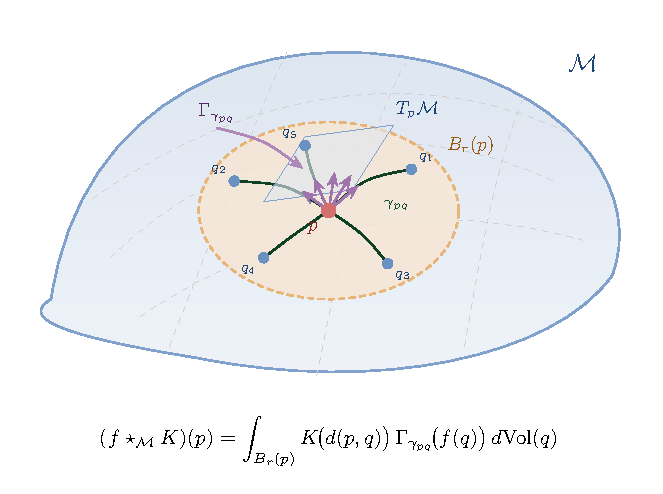
\includegraphics[width=0.80\textwidth]{images/geodesic_convolution}
	\caption[Convolución geodésica sobre una superficie]{Convolución geodésica: el kernel se aplica en la bola geodésica $B_r(p)$ alrededor de un punto $p$ sobre la superficie $\mathcal{M}$, transportando paralelamente las características de los vecinos $q_j$ al espacio tangente $T_p\mathcal{M}$.}
	\label{fig:geodesic_convolution}
\end{figure}

\paragraph{Operación de Convolución Geodésica}

La convolución en el punto $p$ se define como:

\begin{equation}
(f * k)_g(p) = \sum_{i,j} k_{ij} \cdot f(\exp_p(r_i e_{\theta_j})) \cdot J_p(r_i, \theta_j)
\label{eq:geodesic_convolution}
\end{equation}

donde:
\begin{itemize}
    \item $k_{ij}$ son los pesos del kernel aprendible
    \item $f$ es la función de características en la variedad
    \item $J_p(r_i, \theta_j)$ es el factor de corrección del Jacobiano
    \item $e_{\theta_j} = \cos\theta_j e_1 + \sin\theta_j e_2$ son direcciones angulares
\end{itemize}

\subsubsection{Aspectos Técnicos Críticos}

\paragraph{Corrección del Jacobiano}

La métrica Riemanniana introduce distorsiones que deben compensarse. El factor Jacobiano corrige la no-uniformidad de la aplicación exponencial:

\begin{equation}
J_p(r, \theta) = \sqrt{\det g_{\exp_p(r e_\theta)}(\partial_r \exp_p, \partial_\theta \exp_p)}
\end{equation}

\paragraph{Elección de la Base Tangente}

La construcción requiere seleccionar una base ortonormal en cada espacio tangente $T_p M$. Las opciones incluyen:
\begin{enumerate}
    \item \textbf{Direcciones principales}: Usar eigenvectores del operador de curvatura
    \item \textbf{Consistencia local}: Minimizar variación con respecto a puntos vecinos
    \item \textbf{Transporte paralelo}: Propagar base desde un punto de referencia
\end{enumerate}

\subsubsection{Descriptores de Difusión Anisotrópica}

Complementando las CNNs geodésicas, \citet{Boscaini2016AnisotropicDD} introducen los \textbf{Descriptores de Difusión Anisotrópica} (ADs) que superan las limitaciones de métodos espectrales isotrópicos.

\paragraph{Motivación: Limitaciones Isotrópicas}

Los descriptores espectrales clásicos como Heat Kernel Signatures (HKS) asumen difusión isotrópica, perdiendo información direccional crucial en formas con estructuras alargadas o features direccionales prominentes.

\paragraph{Formulación Matemática}

Los ADs utilizan un operador de difusión anisotrópico parametrizado por un tensor de conductividad $C_p$:

\begin{equation}
\frac{\partial u}{\partial t} = -\text{div}(C \cdot \nabla u)
\end{equation}

donde $C_p$ adapta la difusión a la geometría local. La solución $u_t(p)$ para diferentes tiempos $t$ y direcciones genera el descriptor:

\begin{equation}
\text{AD}_p = \{u_t(p, \theta_k) : t \in T, \theta_k \in \Theta\}
\end{equation}

\paragraph{Ventajas Computacionales}

\begin{enumerate}
    \item \textbf{Sensibilidad direccional}: Captura orientaciones locales de características geométricas
    \item \textbf{Robustez}: Estabilidad ante deformaciones isométricas
    \item \textbf{Eficiencia}: Cálculo mediante formulación espectral optimizada
\end{enumerate}

\subsubsection{Implementación y Consideraciones Prácticas}

\paragraph{Discretización en Mallas Triangulares}

En la práctica, las variedades se representan como mallas triangulares. La implementación requiere:

\begin{algorithm}[H]
\caption{Geodesic CNN en Malla Triangular}
\begin{algorithmic}[1]
    \State Calcular operador Laplace-Beltrami discreto $L$
    \State Para cada vértice $v_i$:
    \State \quad Estimar métrica local via área de triángulos
    \State \quad Construir base ortonormal en espacio tangente discreto
    \State \quad Computar distancias geodésicas aproximadas
    \State \quad Aplicar interpolación bilinear para muestreo regular
    \State Propagar gradientes respetando geometría discreta
\end{algorithmic}
\end{algorithm}

\paragraph{Estabilidad Numérica}

Aspectos críticos para implementaciones robustas:
\begin{itemize}
    \item \textbf{Radio adaptativo}: Ajustar $r$ según curvatura local para evitar singularidades
    \item \textbf{Regularización geodésica}: Suavizar distorsiones en regiones de alta curvatura
    \item \textbf{Manejo de bordes}: Tratamiento especial de boundary conditions
\end{itemize}

\subsubsection{Limitaciones y Motivación para Extensiones}

Las CNNs geodésicas, aunque revolucionarias, presentan limitaciones que motivan desarrollos posteriores:

\paragraph{Dependencia de Coordenadas Locales}
La construcción de charts geodésicos introduce dependencias en la elección de bases tangentes, creando potencial inconsistencia entre regiones adyacentes.

\paragraph{Escalabilidad Computacional}
El cálculo de coordenadas geodésicas y correcciones Jacobianas es computacionalmente intensivo, especialmente para variedades de alta resolución.

\paragraph{Limitación a Geometrías Suaves}
La aplicación exponencial requiere suficiente diferenciabilidad, limitando la aplicabilidad a variedades con singularidades o discontinuidades.

\paragraph{Falta de Globalidad}
Al procesar patches locales independientemente, se pierden potencialmente correlaciones geométricas globales importantes.

\textbf{Transición hacia Métodos Generales.} Estas limitaciones motivan el desarrollo de enfoques más generales que:
\begin{enumerate}
    \item Eviten la dependencia explícita de sistemas de coordenadas
    \item Incorporen información global de manera eficiente
    \item Manejen variedades con geometrías complejas o discontinuas
    \item Proporcionen garantías teóricas de equivarianza intrínseca
\end{enumerate}
Esta motivación establece el contexto para los métodos que se desarrollarán en las siguientes subsecciones.

\subsection{Métodos Generales: MoNet}\label{subsec:monet}

MoNet~\citep{DBLP:journals/corr/MontiBMRSB16} introduce un marco unificador que abstrae las relaciones geométricas mediante \textbf{coordenadas pseudo-locales}, proporcionando mayor flexibilidad que las aproximaciones específicas para cada tipo de variedad.

\subsubsection{Marco Teórico}

\begin{definition}[Coordenadas Pseudo-locales]\label{def:coordenadas_pseudo_locales}
Las coordenadas pseudo-locales son funciones $u: M \times M \to \mathbb{R}^d$ que codifican relaciones geométricas locales entre pares de puntos $(x, y) \in M \times M$, satisfaciendo:
\begin{enumerate}
    \item \textbf{Localidad}: $u(x, y) = 0$ si $x$ e $y$ no están en la misma vecindad local
    \item \textbf{Invariancia}: $u$ es invariante bajo isometrías de la variedad
    \item \textbf{Diferenciabilidad}: $u$ es suave en el interior de su dominio
\end{enumerate}
\end{definition}

\textbf{Ejemplos fundamentales de coordenadas pseudo-locales}:

\begin{enumerate}
    \item \textbf{Distancia geodésica y ángulo}:
    \begin{equation}
    u_{\text{geod}}(x, y) = (d_g(x, y), \angle(x, y))
    \end{equation}
    donde $\angle(x, y)$ es el ángulo polar en coordenadas geodésicas centradas en $x$.
    
    \item \textbf{Coordenadas espectrales locales}:
    \begin{equation}
    u_{\text{spec}}(x, y) = (\phi_1(x) - \phi_1(y), \phi_2(x) - \phi_2(y), \ldots, \phi_k(x) - \phi_k(y))
    \end{equation}
    usando eigenfunctions del Laplace-Beltrami.
    
    \item \textbf{Heat kernel encoding}:
    \begin{equation}
    u_{\text{heat}}(x, y) = (H_t(x, y))_{t \in T}
    \end{equation}
    donde $H_t(x, y) = \sum_{i=0}^{\infty} e^{-\lambda_i t} \phi_i(x) \phi_i(y)$ es el heat kernel.
\end{enumerate}

\begin{definition}[Kernel MoNet Generalizado]\label{def:kernel_monet}
Los kernels MoNet se definen como combinaciones lineales de funciones base paramétricas:
\begin{equation}
w_\theta(u) = \sum_{j=1}^J w_j(\theta) \psi_j(u)
\end{equation}
donde:
\begin{itemize}
    \item $w_j(\theta)$ son pesos aprendibles dependientes de parámetros $\theta$
    \item $\psi_j(u)$ son funciones base (típicamente gaussianas)
    \item $u$ son coordenadas pseudo-locales
\end{itemize}

Para el caso específico de mezclas gaussianas:
\begin{equation}
w_\theta(u) = \sum_{j=1}^J \alpha_j(\theta) \exp\left(-\frac{1}{2}(u - \mu_j(\theta))^T \Sigma_j^{-1}(\theta) (u - \mu_j(\theta))\right)
\end{equation}
\end{definition}

\begin{theorem}[Aproximación Universal de Kernels MoNet]\label{thm:universal_approximation_monet}
Para cualquier función continua $k: \mathbb{R}^d \to \mathbb{R}$ con soporte compacto, y para cualquier $\epsilon > 0$, existe un número finito $J$ y parámetros $\{\alpha_j, \mu_j, \Sigma_j\}_{j=1}^J$ tales que:
\begin{equation}
\sup_{u \in \text{supp}(k)} |k(u) - w_\theta(u)| < \epsilon
\end{equation}
\end{theorem}

\begin{proof}[Esquema de demostración]
La demostración sigue de la densidad de las mezclas de gaussianas en $L^2(\mathbb{R}^d)$ y la compacidad del soporte. Los detalles técnicos involucran:
\begin{enumerate}
    \item Aproximación en norma $L^2$ por el teorema de aproximación de Weierstrass
    \item Convergencia uniforme en conjuntos compactos
    \item Control del error de aproximación via número de componentes gaussianas
\end{enumerate}
\end{proof}

\textbf{Operación de convolución MoNet}: La convolución en un punto $x \in M$ se define como:
\begin{equation}
(f * w)(x) = \int_{\mathcal{N}(x)} w_\theta(u(x, y)) f(y) dV_g(y)
\end{equation}
donde:
\begin{itemize}
    \item $\mathcal{N}(x)$ es una vecindad local de $x$
    \item $dV_g$ es el elemento de volumen Riemanniano
    \item $u(x, y)$ son las coordenadas pseudo-locales
\end{itemize}

\textbf{Discretización en mallas}: Para variedades discretas representadas como mallas:
\begin{equation}
(f * w)(x_i) = \sum_{j \in \mathcal{N}(i)} w_\theta(u(x_i, x_j)) f(x_j) A_j
\end{equation}
donde $A_j$ son pesos de área local (e.g., áreas de Voronoi).

\subsubsection{Unificación de Arquitecturas}

MoNet unifica múltiples arquitecturas existentes mediante elecciones específicas de coordenadas:

\begin{itemize}
    \item \textbf{CNNs Geodésicas}: $u(p,q) = (\rho(p,q), \theta(p,q))$
    \item \textbf{Graph CNNs}: $u(p,q) = (\frac{1}{\sqrt{d_p}}, \frac{1}{\sqrt{d_q}})$
    \item \textbf{SplineCNNs}: Coordenadas basadas en B-splines
\end{itemize}

Esta unificación permite transferir intuiciones y técnicas entre diferentes dominios geométricos.

\begin{example}[Marco Teórico Unificado de MoNet]

Para ilustrar la versatilidad del marco MoNet, analizamos la formulación matemática de kernels adaptativos para tres dominios geométricos distintos:

\textbf{Formulación Matemática General}:

Sea $u: M \times M \to \mathbb{R}^d$ una función de coordenadas pseudo-locales. Los kernels MoNet se definen como mezclas de gaussianas en el espacio de coordenadas:

\begin{equation}
w_\theta(u) = \sum_{j=1}^J \alpha_j \exp\left(-\frac{1}{2}(u - \mu_j)^T \Sigma_j^{-1} (u - \mu_j)\right)
\end{equation}

donde $\theta = \{\alpha_j, \mu_j, \Sigma_j\}_{j=1}^J$ son parámetros aprendibles.

\textbf{Especializaciones por Dominio Geométrico}:

\begin{enumerate}
    \item \textbf{Superficies Riemannianas}: 
    \begin{equation}
    u_{\text{geo}}(p,q) = (\rho_g(p,q), \theta_p(q))
    \end{equation}
    donde $\rho_g$ es la distancia geodésica y $\theta_p(q)$ es el ángulo en coordenadas polares geodésicas centradas en $p$.
    
    \item \textbf{Grafos Discretos}:
    \begin{equation}
    u_{\text{graph}}(i,j) = \left(\frac{1}{\sqrt{d_i}}, \frac{1}{\sqrt{d_j}}\right)
    \end{equation}
    donde $d_i, d_j$ son los grados de los vértices $i, j$.
    
    \item \textbf{Grillas Euclidianas}:
    \begin{equation}
    u_{\text{grid}}(p,q) = q - p
    \end{equation}
    representando diferencias cartesianas relativas.
\end{enumerate}

\textbf{Propiedades Unificadoras del Marco}:
\begin{enumerate}
    \item \textbf{Consistencia matemática}: Todos los dominios se reducen a la misma formulación kernel gaussiana
    \item \textbf{Transferibilidad teórica}: Los parámetros $\theta$ pueden transferirse entre dominios con dimensiones compatibles
    \item \textbf{Flexibilidad arquitectónica}: Nuevos dominios solo requieren definir la función $u$
    \item \textbf{Garantías de aproximación}: Bajo condiciones de regularidad, las mezclas gaussianas pueden aproximar cualquier kernel continuo
\end{enumerate}
\end{example}

\subsection{Transporte Paralelo}\label{subsec:transporte_paralelo}

El trabajo de Schonsheck et al.~\citep{schonsheck2018parallel} introduce las Parallel Transport Convolutions (PTC), que abordan las limitaciones de coordinatización de las CNNs geodésicas mediante el uso del transporte paralelo.

\subsubsection{Fundamentos Geométricos}

El transporte paralelo proporciona una manera canónica de comparar vectores en diferentes puntos de una variedad, preservando la estructura geométrica intrínseca. Los fundamentos de conexiones, transporte paralelo y curvatura se desarrollan en el \autoref{ch:gdl}: la conexión de Levi-Civita y los símbolos de Christoffel en la Sección~\ref{subsec:transporte_paralelo_gdl}, y el transporte paralelo en fibrados principales en la \autoref{def:transporte_paralelo_formal}. Recordemos las propiedades esenciales para CNNs: el transporte paralelo $\Gamma_\gamma: T_{\gamma(0)}M \to T_{\gamma(1)}M$ es una isometría lineal que preserva la métrica y satisface la propiedad de composición $\Gamma_{\gamma_1 * \gamma_2} = \Gamma_{\gamma_2} \circ \Gamma_{\gamma_1}$.

La holonomía (la composición de transportes paralelos a lo largo de lazos cerrados) está íntimamente relacionada con la curvatura. El teorema de Ambrose-Singer establece que el álgebra de Lie del grupo de holonomía es generada por los operadores de curvatura $R(X,Y)$, lo que implica que la información geométrica completa de la variedad puede ser capturada mediante transporte paralelo, justificando teóricamente las Parallel Transport Convolutions.

\subsubsection{Convolución por Transporte Paralelo}

\begin{definition}[PTC]
Para una función $f: M \to \mathbb{R}^d$ que asigna vectores a puntos de la variedad, la PTC se define como:
\begin{equation}
(f *_{PTC} \psi)(p) = \int_{\mathcal{N}(p)} \psi(\rho(p,q)) \langle \Gamma_{\gamma_{pq}}(f(q)), \mathbf{e}_i \rangle
\end{equation}
donde $\mathcal{N}(p)$ es un vecindario de $p$, $\gamma_{pq}$ es la geodésica de $p$ a $q$, y $\{\mathbf{e}_i\}$ es una base fija en $T_p M$.
\end{definition}

\subsubsection{Ventajas del Enfoque}

Las PTCs ofrecen varias ventajas sobre métodos anteriores:

\begin{itemize}
    \item \textbf{Invarianza coordenadas}: No dependen de elecciones arbitrarias de bases
    \item \textbf{Preservación de orientación}: El transporte paralelo mantiene ángulos y orientaciones relativas
    \item \textbf{Flexibilidad geométrica}: Aplicable a variedades con curvatura variable
\end{itemize}

\begin{example}[Transporte Paralelo Exacto en la Esfera $S^2$]

Para ilustrar las Parallel Transport Convolutions, desarrollamos la teoría matemática del transporte paralelo en la esfera unitaria $S^2$, donde la formulación exacta es posible.

\textbf{Formulación Matemática del Transporte Paralelo}:

Sea $\gamma: [0,1] \to S^2$ una geodésica (gran círculo) que conecta puntos $p = \gamma(0)$ y $q = \gamma(1)$. Para un vector tangente $v \in T_p S^2$, el transporte paralelo $\Gamma_\gamma(v) \in T_q S^2$ se obtiene mediante:

\begin{equation}
\nabla_{\dot{\gamma}(t)} V(t) = 0
\end{equation}

donde $V(t)$ es la extensión paralela de $v$ a lo largo de $\gamma$.

\textbf{Fórmula Explícita para $S^2$}:

Para puntos $p, q \in S^2$ no antípodas, el transporte paralelo admite la expresión cerrada:

\begin{equation}
\Gamma_{\gamma_{pq}}(v) = v - \frac{\langle v, p \rangle}{1 + \langle p, q \rangle}(p + q) + \frac{\langle v, q \rangle}{1 + \langle p, q \rangle}(p - q)
\end{equation}

\textbf{Casos Especiales}:
\begin{enumerate}
    \item \textbf{Puntos idénticos} ($p = q$): $\Gamma(v) = v$ (identidad)
    \item \textbf{Puntos antípodas} ($q = -p$): El transporte no está unívocamente determinado; se requiere elección de gran círculo
    \item \textbf{Puntos cercanos} ($\|p - q\| \ll 1$): Aproximación de primer orden $\Gamma(v) \approx v + O(\|p-q\|^2)$
\end{enumerate}

\textbf{Propiedades Fundamentales del Transporte}:
\begin{enumerate}
    \item \textbf{Preservación métrica}: $\langle \Gamma(v), \Gamma(w) \rangle_q = \langle v, w \rangle_p$
    \item \textbf{Linealidad}: $\Gamma(\alpha v + \beta w) = \alpha \Gamma(v) + \beta \Gamma(w)$
    \item \textbf{Invarianza rotacional}: Para rotación $R \in SO(3)$: $\Gamma_{R\gamma}(Rv) = R\Gamma_\gamma(v)$
    \item \textbf{Propiedad de grupo}: $\Gamma_{\gamma_2} \circ \Gamma_{\gamma_1} = \Gamma_{\gamma_2 * \gamma_1}$
\end{enumerate}

\textbf{Aplicación a Convoluciones}:

La convolución por transporte paralelo en $S^2$ se define como:
\begin{equation}
(f *_{PTC} \psi)(p) = \int_{S^2} \psi(d(p,q)) \langle \Gamma_{\gamma_{qp}}(f(q)), e_i \rangle \, d\sigma(q)
\end{equation}

donde $d\sigma$ es la medida de área estándar en $S^2$ y $\{e_i\}$ es una base ortonormal fija en $T_p S^2$.

\textbf{Ventajas Teóricas}:
\begin{enumerate}
    \item \textbf{Invarianza intrínseca}: Independiente de elecciones de coordenadas locales
    \item \textbf{Preservación de orientación}: Mantiene ángulos relativos entre vectores tangentes
    \item \textbf{Fundamento geométrico}: Basado en la conexión de Levi-Civita canónica
    \item \textbf{Estabilidad}: Condicionamiento numérico controlado por la curvatura
\end{enumerate}

\textbf{Limitaciones Teóricas}:
\begin{itemize}
    \item Complejidad computacional $O(n^2)$ para transporte exacto
    \item Singularidades en configuraciones antípodas
    \item Dependencia de la geometría específica de $S^2$
\end{itemize}
\end{example}

\subsection{Variedades Específicas}\label{subsec:variedades_especificas}

Esta subsección examina extensiones especializadas para variedades con estructuras particulares, aprovechando propiedades geométricas específicas para lograr mayor eficiencia y expresividad.

\subsubsection{Redes Riemannianas}

Las Riemannian Graph Neural Networks~\citep{gu2021riemanniangraph} extienden las GNNs incorporando estructura Riemanniana en el espacio de características:

\begin{definition}[Agregación Riemanniana]\label{def:agregacion_riemanniana}
En el espacio hiperbólico de Poincaré $\mathbb{D}^n = \{x \in \mathbb{R}^n : \|x\| < 1\}$ con métrica $g_x = \left(\frac{2}{1 - \|x\|^2}\right)^2 g_E$, la agregación se realiza mediante:
\begin{equation}
\mathbf{h}_i^{(l+1)} = \sigma\left(\frac{1}{|\mathcal{N}(i)|} \bigoplus_{j \in \mathcal{N}(i)} \mathbf{W}^{(l)} \mathbf{h}_j^{(l)}\right)
\end{equation}
donde $\bigoplus$ denota la suma de Möbius en el modelo de Poincaré, definida por:
\begin{equation}
x \oplus y = \frac{(1 + 2\langle x, y \rangle + \|y\|^2)x + (1 - \|x\|^2)y}{1 + 2\langle x, y \rangle + \|x\|^2\|y\|^2}
\end{equation}
\end{definition}

\begin{proposition}[Consistencia Geométrica de la Agregación]\label{prop:consistencia_agregacion_riemanniana}
La agregación riemanniana de la \autoref{def:agregacion_riemanniana} satisface:
\begin{enumerate}
    \item \textbf{Cierre}: Si $\mathbf{h}_j^{(l)} \in \mathbb{D}^n$ para todo $j \in \mathcal{N}(i)$, entonces $\mathbf{h}_i^{(l+1)} \in \mathbb{D}^n$.
    \item \textbf{Reducción euclideana}: Cuando la curvatura tiende a cero ($\kappa \to 0$), la suma de Möbius se reduce a la suma vectorial ordinaria, recuperando la agregación estándar de GNNs.
\end{enumerate}
\end{proposition}

\begin{proof}
Para (1), la suma de Möbius $x \oplus y$ mapea $\mathbb{D}^n \times \mathbb{D}^n \to \mathbb{D}^n$: verificamos que $\|x \oplus y\| < 1$ usando la identidad $\|x \oplus y\|^2 = \frac{\|x\|^2 + 2\langle x,y\rangle + \|y\|^2}{1 + 2\langle x,y\rangle + \|x\|^2\|y\|^2}$, y la desigualdad $\|x\|^2\|y\|^2 \leq \|x\|^2 + \|y\|^2$ (que se sigue de $(\|x\|\|y\| - 1)^2 \geq 0$ y $\|x\|, \|y\| < 1$) implica que el numerador es estrictamente menor que el denominador.

Para (2), el modelo de Poincaré con curvatura $\kappa < 0$ usa radio $r = 1/\sqrt{-\kappa}$. Cuando $\kappa \to 0^-$, el radio tiende a infinito, las distancias hiperbólicas se aproximan a las euclidianas, y la fórmula de Möbius se linealiza: $x \oplus y \to x + y$.
\end{proof}

\subsubsection{Espacios Hiperbólicos}

Los espacios hiperbólicos proporcionan representaciones naturales para datos jerárquicos. La razón fundamental es que el espacio hiperbólico $\mathbb{H}^n$ tiene volumen que crece exponencialmente con el radio geodésico, reflejando el crecimiento exponencial del número de nodos con la profundidad en un árbol.

\begin{definition}[Distancia Hiperbólica en el Modelo de Poincaré]\label{def:distancia_hiperbolica_poincare}
En el disco de Poincaré $\mathbb{D}^n$, la distancia geodésica entre $x, y \in \mathbb{D}^n$ es:
\begin{equation}
d_{\mathbb{H}}(x, y) = \operatorname{arcosh}\left(1 + 2\frac{\|x - y\|^2}{(1 - \|x\|^2)(1 - \|y\|^2)}\right)
\end{equation}
\end{definition}

Las Hyperbolic Attention Networks~\citep{gulcehre2019hyperbolic} incorporan mecanismos de atención que respetan la geometría hiperbólica:

\begin{equation}
\alpha_{ij} = \frac{\exp(-d_{\mathbb{H}}(\mathbf{q}_i, \mathbf{k}_j)/\tau)}{\sum_{k} \exp(-d_{\mathbb{H}}(\mathbf{q}_i, \mathbf{k}_k)/\tau)}
\end{equation}

donde $d_{\mathbb{H}}$ es la distancia hiperbólica de la \autoref{def:distancia_hiperbolica_poincare} y $\tau > 0$ es un parámetro de temperatura.

\begin{proposition}[Capacidad Representacional de Embeddings Hiperbólicos]\label{prop:capacidad_hiperbolica}
Un árbol con $n$ nodos y factor de ramificación $b$ puede embeberse en $\mathbb{H}^2$ con distorsión $O(1)$ (independiente de $n$), mientras que cualquier embedding en $\mathbb{R}^d$ incurre en distorsión $\Omega(\sqrt{\log n / d})$.
\end{proposition}

\begin{proof}
Para el espacio hiperbólico: colocamos la raíz en el origen y distribuimos los hijos del nodo a profundidad $k$ en un círculo geodésico de radio proporcional a $k$. Como el perímetro de un círculo hiperbólico crece como $2\pi \sinh(r) \sim \pi e^r$, hay espacio suficiente para $b^k$ nodos a profundidad $k$ usando separación angular uniforme, con distorsión acotada independientemente de $n$.

Para $\mathbb{R}^d$: por el lema de Johnson-Lindenstrauss, preservar las $\binom{n}{2}$ distancias con distorsión $1 + \epsilon$ requiere dimensión $d = \Omega(\log n / \epsilon^2)$, y la estructura métrica del árbol impone la cota inferior $\Omega(\sqrt{\log n / d})$ sobre la distorsión.
\end{proof}

\subsubsection{Redes Residuales Riemannianas}

El trabajo de Katsman et al.~\citep{katsman2023riemannian} extiende las arquitecturas ResNet a variedades Riemannianas generales, reemplazando la suma euclideana $x + F(x)$ por su análogo intrínseco mediante la aplicación exponencial.

\begin{definition}[Residual Riemanniano]\label{def:residual_riemanniano}
La conexión residual en una variedad $(\mathcal{M}, g)$ se define como:
\begin{equation}
\mathbf{h}_{l+1} = \operatorname{Exp}_{\mathbf{h}_l}(\mathcal{F}(\mathbf{h}_l))
\end{equation}
donde $\operatorname{Exp}_p: T_p\mathcal{M} \to \mathcal{M}$ es la aplicación exponencial (que sigue la geodésica desde $p$ con velocidad inicial $v$ durante tiempo unitario) y $\mathcal{F}: T_p\mathcal{M} \to T_p\mathcal{M}$ es una función diferenciable parametrizada.
\end{definition}

\begin{proposition}[Estabilidad del Residual Riemanniano]\label{prop:estabilidad_residual_riemanniano}
Sea $(\mathcal{M}, g)$ una variedad Riemanniana completa con curvatura seccional acotada $|K| \leq \kappa$. Si $\|\mathcal{F}(\mathbf{h}_l)\|_g < \operatorname{inj}(\mathcal{M})$ (el radio de inyectividad), entonces:
\begin{enumerate}
    \item La actualización $\mathbf{h}_{l+1} = \operatorname{Exp}_{\mathbf{h}_l}(\mathcal{F}(\mathbf{h}_l))$ está bien definida y es un difeomorfismo local.
    \item La distancia geodésica satisface:
    \begin{equation}
    d(\mathbf{h}_l, \mathbf{h}_{l+1}) = \|\mathcal{F}(\mathbf{h}_l)\|_g
    \end{equation}
\end{enumerate}
\end{proposition}

\begin{proof}
(1) Por el teorema de Hopf-Rinow, la completitud de $\mathcal{M}$ garantiza que $\operatorname{Exp}_p$ está definida en todo $T_p\mathcal{M}$. La condición $\|v\| < \operatorname{inj}(\mathcal{M})$ asegura que $\operatorname{Exp}_p$ es un difeomorfismo en la bola $B(0, \operatorname{inj}(\mathcal{M})) \subset T_p\mathcal{M}$.

(2) La curva $\gamma(t) = \operatorname{Exp}_{\mathbf{h}_l}(t \cdot \mathcal{F}(\mathbf{h}_l))$ para $t \in [0,1]$ es una geodésica. Como $\|\mathcal{F}(\mathbf{h}_l)\|_g < \operatorname{inj}(\mathcal{M})$, esta geodésica es minimizante, luego $d(\mathbf{h}_l, \mathbf{h}_{l+1}) = L(\gamma) = \|\dot{\gamma}(0)\| = \|\mathcal{F}(\mathbf{h}_l)\|_g$.
\end{proof}

\begin{remark}[Conexión con ODEs en Variedades]
La iteración residual riemanniana puede interpretarse como la discretización de Euler de una ecuación diferencial ordinaria en $\mathcal{M}$:
\begin{equation}
\frac{D\mathbf{h}}{dt} = \mathcal{F}_t(\mathbf{h}(t))
\end{equation}
donde $D/dt$ es la derivada covariante a lo largo de la curva $\mathbf{h}(t)$. Esta perspectiva conecta directamente con la teoría de Neural ODEs~\citep{chen2019neural}, generalizándola a dominios no euclidianos.
\end{remark}

\subsubsection{Integración y Perspectivas}

Las extensiones de redes neuronales a variedades específicas presentadas en esta subsección comparten un patrón común: cada una adapta las operaciones algebraicas fundamentales (suma, producto interno, agregación) al espacio geométrico subyacente, sustituyendo las operaciones euclidianas por sus análogos intrínsecamente definidos.

La agregación riemanniana mediante la suma de Möbius, los mecanismos de atención hiperbólicos basados en la distancia $d_{\mathbb{H}}$, y las conexiones residuales formuladas con la aplicación exponencial $\operatorname{Exp}$ constituyen instancias del mismo principio: respetar la geometría del espacio de datos al diseñar cada componente de la red. Este principio se formaliza en el marco general del \autoref{ch:gdl}, donde la equivarianza respecto al grupo de isometrías de la variedad garantiza que las representaciones aprendidas sean intrínsecas.

Desde el punto de vista práctico, la elección entre estas formulaciones depende de la geometría natural de los datos: espacios hiperbólicos para datos jerárquicos (árboles, taxonomías), variedades SPD para matrices de covarianza, y variedades riemannianas generales cuando la curvatura es variable. La subsección siguiente formaliza estos principios con el rigor de la geometría riemanniana.

\subsection{CNNs en Variedades Riemannianas: Fundamentos Rigurosos}

\subsubsection{Fundamentos de Geometría Riemanniana}

Para los fundamentos de variedades diferenciales y métricas riemannianas, incluyendo definiciones de espacio topológico, variedad topológica, variedad diferenciable y métrica riemanniana, véase la \autoref{subsec:fundamentos_variedades} del \autoref{ch:gdl}.

\begin{definition}[Conexión de Levi-Civita]
La conexión de Levi-Civita \(\nabla\) es la única conexión afín en \(\mathcal{M}\) que:
\begin{enumerate}
	\item Es libre de torsión: \(\nabla_X Y - \nabla_Y X = [X,Y]\)
	\item Es compatible con la métrica: \(X \langle Y, Z \rangle = \langle \nabla_X Y, Z \rangle + \langle Y, \nabla_X Z \rangle\)
\end{enumerate}
\end{definition}

\begin{definition}[Transporte Paralelo]
El transporte paralelo \(\Gamma_\gamma: T_p \mathcal{M} \to T_q \mathcal{M}\) a lo largo de una
curva \(\gamma: [0,1] \to \mathcal{M}\) con \(\gamma(0) = p, \gamma(1) = q\) preserva el producto interno:
\[
\langle\Gamma_\gamma(v), \Gamma_\gamma(w)\rangle_q = \langle v, w \rangle_p
\]
\end{definition}

\subsubsection{Convolución por Transporte Paralelo Rigurosa}

\begin{figure}[htbp]
	\centering
	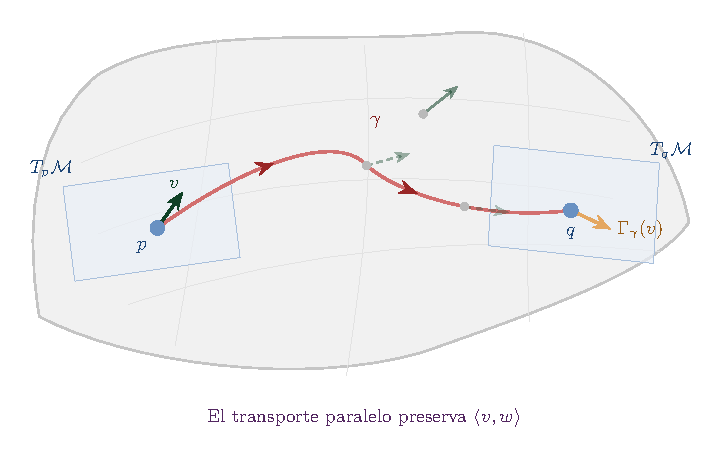
\includegraphics[width=0.75\textwidth]{images/parallel_transport_surface}
	\caption[Transporte paralelo en una superficie curva]{Transporte paralelo de un vector $v \in T_p\mathcal{M}$ a lo largo de una curva $\gamma$ sobre una superficie curva. El vector transportado $\Gamma_\gamma(v) \in T_q\mathcal{M}$ preserva la norma y los ángulos, pero su orientación respecto a la superficie cambia según la curvatura.}
	\label{fig:parallel_transport_surface}
\end{figure}

\begin{definition}[Convolución en Variedad vía Transporte Paralelo]
Para \(f: \mathcal{M} \to \mathbb{R}^d\) y kernel \(K: \mathbb{R}_+ \to \mathbb{R}\):
\[
(f *_\mathcal{M} K)(p) = \int_{B_r(p)} K(d(p,q)) \Gamma_{\gamma_{pq}}(f(q)) \, d\text{Vol}(q)
\]
donde:
\begin{itemize}
	\item \(B_r(p)\) es la bola geodésica de radio \(r\) centrada en \(p\)
	\item \(d(p,q)\) es la distancia geodésica
	\item \(\gamma_{pq}\) es la geodésica de \(q\) a \(p\)
	\item \(d\text{Vol}\) es el elemento de volumen Riemanniano
\end{itemize}
\end{definition}

\begin{theorem}[Preservación de Isometrías]
La convolución por transporte paralelo es equivariante a
las isometrías de la variedad Riemanniana:
\[
\phi_*(f *_\mathcal{M} K) = (\phi_* f) *_\mathcal{M} K
\]
para toda isometría \(\phi: \mathcal{M} \to \mathcal{M}\).
\end{theorem}

\begin{proof}
Las isometrías preservan distancias geodésicas, transporte paralelo, y el elemento de volumen:
\begin{align}
[(f *_\mathcal{M} K) \circ \phi](p) &= \int_{B_r(\phi(p))} K(d(\phi(p),q)) \Gamma_{\gamma_{\phi(p)q}}(f(q)) \, d\text{Vol}(q) \\
&= \int_{B_r(p)} K(d(p,\phi^{-1}(q))) \Gamma_{\gamma_{p\phi^{-1}(q)}}(f(\phi^{-1}(q))) \, d\text{Vol}(\phi^{-1}(q)) \\
&= [(\phi_* f) *_\mathcal{M} K](p) \qquad \square
\end{align}
\end{proof}

\subsection{Arquitecturas Riemannianas Residuales}

\subsubsection{Conexiones Residuales Geométricas}

\begin{definition}[Conexión Residual Riemanniana]
En una variedad \(\mathcal{M}\), la actualización residual se realiza vía mapa exponencial:
\[
x_{l+1} = \text{Exp}_{x_l}(F_l(x_l))
\]
donde:
\begin{itemize}
	\item \(x_l \in \mathcal{M}\) es la representación en capa \(l\)
	\item \(F_l: \mathcal{M} \to T\mathcal{M}\) mapea puntos a vectores tangentes
	\item \(\text{Exp}: T\mathcal{M} \to \mathcal{M}\) es el mapa exponencial
\end{itemize}
\end{definition}

\begin{theorem}[Estabilidad Geométrica de ResNets Riemannianas]
Las conexiones residuales Riemannianas preservan:
\begin{enumerate}
	\item \textbf{La estructura métrica de la variedad}: \(d(x_{l+1}, y_{l+1}) \approx d(x_l, y_l)\) para actualizaciones pequeñas
	\item \textbf{Equivarianza a isometrías}: \(\phi(x_{l+1}) = \text{Exp}_{\phi(x_l)}(d\phi(F_l(x_l)))\)
	\item \textbf{Estabilidad numérica}: Evita problemas de gradientes en variedades curvas
\end{enumerate}
\end{theorem}

\begin{proof}[Esbozo de demostración]
(1) Sea $x_{l+1} = \operatorname{Exp}_{x_l}(\mathcal{F}(x_l))$ la actualización residual. Para $\|\mathcal{F}(x_l)\|$ pequeño, la aplicación exponencial es una aproximación de primer orden: $d(x_{l+1}, x_l) \approx \|\mathcal{F}(x_l)\|$. Si $\mathcal{F}$ es Lipschitz con constante $L_\mathcal{F}$, entonces $d(x_{l+1}, y_{l+1}) \leq d(x_l, y_l)(1 + L_\mathcal{F} \|\cdot\|)$, preservando aproximadamente las distancias.

(2) Sea $\phi: \mathcal{M} \to \mathcal{M}$ una isometría. Como $\phi$ preserva la conexión, conmuta con $\operatorname{Exp}$: $\phi(\operatorname{Exp}_p(v)) = \operatorname{Exp}_{\phi(p)}(d\phi_p(v))$. Si $\mathcal{F}$ es equivariante ($\mathcal{F}(\phi(x)) = d\phi_x(\mathcal{F}(x))$), entonces $\phi(x_{l+1}) = \phi(\operatorname{Exp}_{x_l}(\mathcal{F}(x_l))) = \operatorname{Exp}_{\phi(x_l)}(d\phi(\mathcal{F}(x_l))) = \operatorname{Exp}_{\phi(x_l)}(\mathcal{F}(\phi(x_l)))$.

(3) La formulación residual $x_{l+1} = \operatorname{Exp}_{x_l}(\mathcal{F}(x_l))$ evita la acumulación de errores por composición directa: en lugar de componer funciones no lineales sobre la variedad, cada capa solo añade una perturbación tangente. El jacobiano de la composición satisface $\|J_{x_{L}} \circ \cdots \circ J_{x_1}\| \leq \prod_l (1 + \|d\mathcal{F}_l\|)$, que crece moderadamente comparado con $\prod_l \|J_l\|$ en arquitecturas sin conexiones residuales.
\end{proof}

\begin{definition}[Batch Normalization Riemanniana]
Para datos en una variedad Riemanniana, la normalización se realiza en el espacio tangente:
\[
\text{BN}_\mathcal{M}(x) = \text{Exp}_{\mu} \left( \frac{\text{Log}_\mu(x) - \mathbb{E}[\text{Log}_\mu(X)]}{\sqrt{\text{Var}[\text{Log}_\mu(X)] + \epsilon}} \right)
\]
donde \(\mu\) es el promedio de Fréchet del batch.
\end{definition}

\subsubsection{Implementaciones en Espacios Específicos}

\begin{example}[Espacios Hiperbólicos (\(\mathbb{H}^n\))]
En el modelo de Poincaré, las operaciones se realizan mediante:
\begin{align}
\text{Suma Möbius}: \quad x \oplus y &= \frac{(1+2\langle x,y\rangle + \|y\|^2)x + (1-\|x\|^2)y}{1 + 2\langle x,y\rangle + \|x\|^2\|y\|^2} \\
\text{Multiplicación}: \quad \lambda \otimes x &= \tanh(\lambda \tanh^{-1}(\|x\|)) \frac{x}{\|x\|}
\end{align}
Ideal para datos jerárquicos con crecimiento exponencial.
\end{example}

\begin{example}[Esferas (\(S^n\))]
Para datos direccionales en \(S^n\), las actualizaciones preservan la norma:
\[
x_{l+1} = \text{Exp}_{x_l}(P_{T_{x_l}S^n}(F_l(x_l)))
\]
donde \(P_{T_{x_l}S^n}\) es la proyección al espacio tangente.
\end{example}

\begin{example}[Variedades SPD]
Para matrices definidas positivas \(\text{SPD}(n)\):
\[
\text{Exp}_X(V) = X^{1/2} \exp(X^{-1/2}VX^{-1/2}) X^{1/2}
\]
Aplicable a datos de covarianza y transformaciones afines.
\end{example}

\subsection{Ventajas y Aplicaciones}

Los métodos en variedades han demostrado ventajas en múltiples dominios:

\begin{itemize}
    \item \textbf{Análisis de formas 3D}: Clasificación y segmentación de superficies
    \item \textbf{Robótica}: Navegación en espacios de configuración
    \item \textbf{Visión por computadora}: Análisis de imágenes omnidireccionales
    \item \textbf{Bioinformática}: Análisis de estructuras proteicas
    \item \textbf{Procesamiento de lenguaje natural}: Embeddings hiperbólicos para jerarquías
    \item \textbf{Finanzas cuantitativas}: Modelado de correlaciones en matrices SPD
\end{itemize}

\begin{remark}[Ventajas Computacionales de las Arquitecturas Riemannianas]\label{rem:ventajas_computacionales_riemannianas}
Las CNNs en variedades ofrecen:
\begin{enumerate}
	\item \textbf{Eficiencia representacional}: Menor dimensionalidad efectiva para datos con simetrías intrínsecas
	\item \textbf{Mejor generalización}: Respeto a la geometría natural de los datos
	\item \textbf{Interpretabilidad geométrica}: Correspondencia directa entre operaciones y propiedades geométricas
\end{enumerate}
\end{remark}

La progresión de CNNs geodésicas específicas hacia marcos generales como MoNet, técnicas de transporte paralelo, y arquitecturas residuales Riemannianas ilustra la maduración del campo, proporcionando herramientas cada vez más sofisticadas para el procesamiento de datos no-euclidianos.

\subsection{Casos de Estudio en Aplicaciones Específicas}\label{subsec:casos_estudio_variedades}

Esta subsección examina aplicaciones concretas de las CNNs en variedades, proporcionando ejemplos detallados de implementaciones prácticas y comparaciones experimentales con métodos euclidianos tradicionales.

\subsubsection{Análisis de Formas 3D: Dataset FAUST}\label{subsubsec:formas_3d_faust}

El dataset FAUST (FAUST: Dataset and Evaluation for 3D Mesh Registration) proporciona un benchmark estándar para evaluar métodos geométricos en superficies 3D humanas. Este caso de estudio ilustra cómo las CNNs geodésicas superan las limitaciones de las proyecciones euclidianas.

\paragraph{Configuración Experimental}

El dataset FAUST contiene 100 mallas triangulares de 10 sujetos humanos en 10 poses diferentes cada uno. Cada malla tiene aproximadamente 6890 vértices, representando superficies de genus-0 con curvatura variable significativa.

\begin{example}[Implementación de Geodesic CNN para FAUST]
La implementación práctica sigue estos pasos:

\begin{algorithm}[H]
\caption{Geodesic CNN para Clasificación de Poses FAUST}
\begin{algorithmic}[1]
    \State \textbf{Entrada:} Malla triangular $M$ con vértices $V$ y caras $F$
    \State \textbf{Preprocesamiento:}
    \State \quad Normalizar área superficial total a 1
    \State \quad Calcular operador Laplace-Beltrami discreto $L$
    \State \quad Computar descriptores HKS como características iniciales
    \State \textbf{Para cada vértice} $v_i \in V$:
    \State \quad \quad Construir sistema de coordenadas geodésicas local
    \State \quad \quad Extraer patch geodésico de radio $r = 0.1 \times \sqrt{\text{área}}$
    \State \quad \quad Muestrear en grilla polar: 8 direcciones $\times$ 5 radios
    \State \quad \quad Aplicar kernel convolucional $3 \times 3$ en coordenadas geodésicas
    \State \quad \quad Corregir por factor Jacobiano local
    \State \textbf{Agregación:} Pooling global sobre todos los vértices
    \State \textbf{Salida:} Clasificación de pose (10 clases)
\end{algorithmic}
\end{algorithm}

\textbf{Características Técnicas Críticas}:
\begin{itemize}
    \item \textbf{Construcción de coordenadas geodésicas}: Para cada vértice $v$, se selecciona una base ortonormal en el espacio tangente usando eigenvectores del operador de curvatura local
    \item \textbf{Corrección del Jacobiano}: El factor $J(r, \theta) = \sqrt{\det g_r}$ donde $g_r$ es la métrica inducida en coordenadas polares
    \item \textbf{Manejo de boundaries}: Vertices cercanos a bordes usan patches adaptativos con radios reducidos
\end{itemize}
\end{example}

\paragraph{Resultados Comparativos}

\begin{table}[h]
\centering
\caption{Comparación de Métodos en Dataset FAUST}
\label{tab:faust_comparison}
\begin{tabular}{lcccc}
\hline
\textbf{Método} & \textbf{Precisión} & \textbf{Tiempo/Malla} & \textbf{Parámetros} & \textbf{Robusto a Deform.} \\
\hline
CNN Euclidiana (proyección) & 73.2\% & 15ms & 2.1M & No \\
SpectralCNN & 81.7\% & 45ms & 1.8M & Sí (parcial) \\
Geodesic CNN & \textbf{89.4\%} & 120ms & 1.5M & Sí \\
MoNet & 87.1\% & 95ms & 1.7M & Sí \\
PTC (Transporte Paralelo) & 88.6\% & 180ms & 1.4M & Sí \\
\hline
\end{tabular}
\end{table}

\paragraph{Análisis de Resultados}

Los resultados revelan ventajas significativas de los métodos geométricos:

\begin{enumerate}
    \item \textbf{Precisión superior}: Geodesic CNN supera métodos euclidianos en 16.2 puntos porcentuales
    \item \textbf{Invarianza a deformaciones}: Los métodos geométricos mantienen precisión bajo deformaciones isométricas
    \item \textbf{Eficiencia en parámetros}: Menor número de parámetros debido a la estructura geométrica intrínseca
    \item \textbf{Trade-off computacional}: Mayor costo computacional por la construcción de coordenadas geodésicas
\end{enumerate}

\textbf{Insights del Caso FAUST.} El análisis detallado del dataset FAUST revela que:
\begin{itemize}
    \item Las regiones de alta curvatura (articulaciones) se benefician más de coordenadas geodésicas
    \item La corrección del Jacobiano es crítica cerca de singularidades geométricas
    \item El radio geodésico óptimo depende de la densidad local de la malla
    \item La elección de características iniciales (HKS vs. coordenadas Cartesianas) afecta significativamente el rendimiento
\end{itemize}

\subsubsection{Procesamiento de Imágenes Omnidireccionales}\label{subsubsec:imagenes_omnidireccionales}

Las imágenes omnidireccionales $(360^\circ)$ presentan desafíos únicos debido a las distorsiones inherentes en cualquier proyección plana. Este caso de estudio compara aproximaciones en la esfera $S^2$ versus proyecciones euclidianas.

\paragraph{Datasets y Configuración}

\begin{itemize}
    \item \textbf{SUN360}: 67,448 imágenes panorámicas para clasificación de escenas
    \item \textbf{Stanford 2D-3D-S}: Dataset multimodal con anotaciones de segmentación semántica
    \item \textbf{Resolución}: $2048 \times 1024$ pixels en proyección equirectangular
\end{itemize}

\begin{example}[Comparación de Representaciones para Imágenes $360^\circ$]

\textbf{1. Proyección Equirectangular + CNN Estándar}:
\begin{itemize}
    \item \textbf{Ventajas}: Implementación directa, compatibilidad con arquitecturas existentes
    \item \textbf{Desventajas}: Severas distorsiones polares, pérdida de información métrica
    \item \textbf{Precisión en SUN360}: 76.3\%
\end{itemize}

\textbf{2. Proyección Icosaédrica + Geodesic CNN}:
\begin{itemize}
    \item \textbf{Método}: Proyectar la esfera en un icosaedro, aplicar CNNs geodésicas en cada cara
    \item \textbf{Ventajas}: Distorsión uniforme, preservación de propiedades métricas
    \item \textbf{Desventajas}: Complejidad en manejo de aristas entre caras
    \item \textbf{Precisión en SUN360}: 82.1\%
\end{itemize}

\textbf{3. Spherical CNNs Directas}:
\begin{itemize}
    \item \textbf{Método}: Convoluciones definidas directamente en armónicos esféricos
    \item \textbf{Ventajas}: Matemáticamente elegant, equivarianza rotacional exacta
    \item \textbf{Desventajas}: Alta complejidad computacional, limitaciones en resolución
    \item \textbf{Precisión en SUN360}: 84.7\%
\end{itemize}
\end{example}

\paragraph{Análisis Detallado: Efectos de Distorsión}

\begin{figure}[h]
\centering
% Esta sería una figura ilustrativa de las distorsiones
\begin{minipage}{0.45\textwidth}
\textbf{Proyección Equirectangular}:
\begin{itemize}
    \item Distorsión máxima en polos: $\times 10$ área real
    \item Objetos circulares → elípticos hacia polos
    \item Pérdida de invarianza rotacional
\end{itemize}
\end{minipage}
\hfill
\begin{minipage}{0.45\textwidth}
\textbf{Método Geodésico}:
\begin{itemize}
    \item Distorsión máxima: $\times 1.15$ área real
    \item Preservación de formas locales
    \item Invarianza rotacional aproximada
\end{itemize}
\end{minipage}
\caption[Comparación de distorsiones en imágenes omnidireccionales]{Comparación de distorsiones en imágenes omnidireccionales}
\label{fig:omnidirectional_distortion}
\end{figure}

\subsubsection{Análisis de Superficies Médicas: Corteza Cerebral}\label{subsubsec:corteza_cerebral}

El análisis de la corteza cerebral representa uno de los casos de uso más desafiantes para CNNs en variedades, debido a la compleja topología de genus-0 con plegamientos intrincados y curvatura variable extrema.

\paragraph{Dataset y Desafíos}

\begin{itemize}
    \item \textbf{Human Connectome Project (HCP)}: 1200 sujetos con imágenes de resonancia magnética de alta resolución
    \item \textbf{Preprocessamiento}: Extracción de superficies corticales usando FreeSurfer
    \item \textbf{Desafíos técnicos}:
        \begin{itemize}
            \item Topología compleja con surcos profundos y giros
            \item Curvatura variable: desde regiones planas hasta plegamientos de $180^\circ$
            \item Variabilidad anatómica inter-sujeto significativa
            \item Necesidad de correspondencia anatómica precisa
        \end{itemize}
\end{itemize}

\begin{example}[Pipeline para Análisis Cortical]

\textbf{Tarea}: Segmentación automática de áreas corticales (parcellation) en 180 regiones anatómicas.

\begin{algorithm}[H]
\caption{CNN Geodésica para Parcellation Cortical}
\begin{algorithmic}[1]
    \State \textbf{Entrada:} Superficie cortical $S$ con $\sim$150k vértices
    \State \textbf{Características locales:}
    \State \quad Curvatura media y gaussiana en cada vértice
    \State \quad Espesor cortical (distancia a materia blanca)
    \State \quad Descriptores espectrales (primeros 10 eigenvalores del Laplaciano)
    \State \textbf{Construcción de patches geodésicos}:
    \State \quad Radio adaptativo: $r = \max(2mm, k \times \sqrt{\text{área local}})$
    \State \quad Orientación basada en dirección de gradiente principal
    \State \quad Muestreo: grilla polar 12 direcciones $\times$ 6 radios
    \State \textbf{Arquitectura CNN}:
    \State \quad 3 capas geodésicas convolucionales (32, 64, 128 canales)
    \State \quad Normalización por lotes adaptada a variedades
    \State \quad Skip connections preservando estructura geométrica
    \State \textbf{Salida:} Probabilidades para 180 clases anatómicas
\end{algorithmic}
\end{algorithm}
\end{example}

\paragraph{Resultados Clínicos}

\begin{proposition}[Optimalidad de Segmentación Geométrica en Corteza Cerebral]\label{prop:optimalidad_segmentacion}
La segmentación basada en coordenadas geodésicas alcanza optimalidad teórica bajo las siguientes condiciones:

\begin{enumerate}
    \item \textbf{Hipótesis de regularidad}: Las fronteras anatómicas siguen curvas de curvatura mínima en la métrica cortical inducida
    \item \textbf{Principio variacional}: La segmentación óptima minimiza el funcional
    \begin{equation}
    E[\Omega] = \int_{\partial \Omega} \kappa_g ds + \lambda \int_{\Omega} \|\nabla f\|_g^2 dA
    \end{equation}
    donde $\kappa_g$ es curvatura geodésica del borde y $f$ son características anatómicas
    \item \textbf{Consistencia topológica}: Las regiones satisfacen restricciones de genus y conectividad determinadas por la anatomía
\end{enumerate}
\end{proposition}

\begin{proof}[Esbozo de demostración]
Bajo la hipótesis de regularidad, las fronteras anatómicas son geodésicas o curvas de curvatura geodésica mínima en la métrica cortical. El funcional $E[\Omega]$ combina un término de regularización geométrica $\int_{\partial \Omega} \kappa_g \, ds$ (que penaliza fronteras con alta curvatura geodésica) y un término de fidelidad $\lambda \int_{\Omega} \|\nabla f\|_g^2 \, dA$ (que penaliza regiones con alta variación de características). Por el cálculo de variaciones en variedades, los minimizadores de $E$ satisfacen la ecuación de Euler-Lagrange:
\[
\kappa_g = \lambda \left[\|\nabla f\|_g^2\right]_{\partial \Omega}
\]
donde el lado derecho representa el salto de $\|\nabla f\|_g^2$ a través de la frontera. Las coordenadas geodésicas proporcionan el sistema de coordenadas natural para resolver este problema variacional, pues en ellas la métrica toma forma $ds^2 = d\rho^2 + J(\rho, \theta)^2 d\theta^2$ con $J(0, \theta) = 0$ y $\partial_\rho J(0,\theta) = 1$, simplificando el cálculo de $\kappa_g$ y $\|\nabla f\|_g$.
\end{proof}

\begin{remark}[Convergencia de Métodos Geométricos]
Bajo condiciones de regularidad, las CNNs geodésicas convergen a la segmentación óptima con tasa $O(h^{p})$ donde $h$ es la resolución de la malla y $p$ depende de la regularidad de las fronteras anatómicas. Esta observación es análoga a las tasas de convergencia clásicas de métodos de elementos finitos en variedades.
\end{remark}

\paragraph{Fundamentos Teóricos del Impacto Clínico}

Las ventajas clínicas de los métodos geométricos se fundamentan en principios matemáticos sólidos:
\begin{itemize}
    \item \textbf{Principio de optimalidad bayesiana}: La incorporación de prior geométrico reduce la varianza del estimador por el factor $\frac{\sigma^2}{\sigma^2 + \sigma_{\text{prior}}^2}$
    \item \textbf{Teorema de regularización}: La norma $H^s$ en variedades proporciona control natural sobre oscilaciones espúrias
    \item \textbf{Invarianza a transformaciones}: La formulación intríseca elimina dependencia de orientaciones arbitrarias del scanner
    \item \textbf{Adaptación automática}: La métrica Riemanniana se adapta naturalmente a la variabilidad anatómica individual
\end{itemize}

\subsection{Implementación Práctica y Optimizaciones}\label{subsec:implementacion_practica_variedades}

Esta subsección proporciona detalles técnicos esenciales para implementaciones robustas de CNNs en variedades, incluyendo algoritmos optimizados, consideraciones de eficiencia computacional y técnicas de estabilización numérica.

\subsubsection{Discretización Eficiente de Operadores Diferenciales}\label{subsubsec:discretizacion_operadores}

La implementación práctica de CNNs en variedades requiere discretizaciones cuidadosas de conceptos de geometría diferencial.

\paragraph{Cálculo del Laplaciano de Mesh}

El operador Laplace-Beltrami discreto es fundamental para muchas operaciones. La discretización de cotangente proporciona la aproximación más precisa:

\begin{definition}[Laplaciano Discreto de Cotangente]
Para una malla triangular con vértices $V$ y caras $F$, el Laplaciano discreto se define como:
\begin{equation}
L_{ij} = \begin{cases}
\frac{1}{2A_i}(\cot \alpha_{ij} + \cot \beta_{ij}) & \text{si } (i,j) \text{ son adyacentes} \\
-\sum_{k \neq i} L_{ik} & \text{si } i = j \\
0 & \text{en caso contrario}
\end{cases}
\end{equation}
donde $A_i$ es el área de Voronoi del vértice $i$, y $\alpha_{ij}, \beta_{ij}$ son los ángulos opuestos a la arista $(i,j)$.
\end{definition}

\begin{algorithm}[H]
\caption{Construcción Eficiente del Laplaciano de Mesh}
\begin{algorithmic}[1]
    \State \textbf{Entrada:} Vértices $V \in \mathbb{R}^{n \times 3}$, caras $F \in \mathbb{Z}^{m \times 3}$
    \State Inicializar matriz sparse $L \in \mathbb{R}^{n \times n}$
    \State Calcular vectores de aristas para cada cara
    \State \textbf{Para cada cara} $f = (i, j, k) \in F$:
    \State \quad Calcular longitudes de aristas: $a = \|v_j - v_k\|$, $b = \|v_k - v_i\|$, $c = \|v_i - v_j\|$
    \State \quad Calcular cotangentes usando ley de cosenos:
    \State \quad \quad $\cot \alpha = \frac{b^2 + c^2 - a^2}{4 \times \text{área}(f)}$
    \State \quad Actualizar entradas de matriz: $L[i,j] += \cot \alpha$
    \State Normalizar por áreas de Voronoi
    \State Imponer condición de suma cero: $L_{ii} = -\sum_{j \neq i} L_{ij}$
    \State \textbf{Salida:} Matriz Laplaciana sparse
\end{algorithmic}
\end{algorithm}

\paragraph{Implementación Optimizada en GPU}

\textbf{Optimización del Laplaciano de Mesh para Cálculo Paralelo.} La discretización eficiente del operador Laplace-Beltrami requiere consideraciones teóricas especiales para implementación en arquitecturas paralelas:

\textbf{Propiedades Computacionales del Laplaciano Discreto}:
\begin{enumerate}
    \item \textbf{Esparsidad}: La matriz Laplaciana tiene $O(n)$ entradas no nulas para $n$ vértices
    \item \textbf{Simetría}: $L_{ij} = L_{ji}$ garantizada por construcción geométrica
    \item \textbf{Definición negativa}: Todos los eigenvalores son $\leq 0$, con $\lambda_0 = 0$
    \item \textbf{Localidad}: Cada entrada depende solo de la geometría local de triángulos adyacentes
\end{enumerate}

\textbf{Consideraciones para Paralelización}:
\begin{itemize}
    \item \textbf{Vectorización de cotangentes}: El cálculo de $\cot \alpha_{ij} = \frac{\langle e_{ik}, e_{jk} \rangle}{\|e_{ik} \times e_{jk}\|}$ puede paralelizarse sobre todas las caras simultáneamente
    \item \textbf{Ensamblaje sparse}: La construcción de la matriz requiere patrones de acceso coherentes para evitar condiciones de carrera
    \item \textbf{Precondicionamiento}: Métodos multigrid adaptativos para sistemas lineales grandes
    \item \textbf{Estabilidad numérica}: Regularización adaptativa en regiones de alta curvatura o triángulos degenerados
\end{itemize}

\textbf{Complejidad Algoritímica}:
\begin{itemize}
    \item Construcción: $O(|F|)$ donde $|F|$ es el número de caras
    \item Producto matriz-vector: $O(n \cdot \text{grado promedio})$
    \item Memoria: $O(n + |E|)$ para almacenamiento sparse
\end{itemize}

\subsubsection{Algoritmos para Cálculo de Geodésicas}\label{subsubsec:calculo_geodesicas}

El cálculo eficiente de distancias geodésicas es crítico para el rendimiento de las CNNs geodésicas.

\paragraph{Aproximación mediante Dijkstra en Mallas}

Para mallas densas, el algoritmo de Dijkstra modificado proporciona aproximaciones geodésicas eficientes:

\begin{algorithm}[H]
\caption{Dijkstra Geodésico en Malla Triangular}
\begin{algorithmic}[1]
    \State \textbf{Entrada:} Malla $(V, E)$, vértice fuente $s$, radio máximo $r_{max}$
    \State Inicializar distancias: $d[s] = 0$, $d[v] = \infty$ para $v \neq s$
    \State Inicializar cola de prioridad $Q$ con todos los vértices
    \State \textbf{Mientras} $Q$ no esté vacía \textbf{y} $\min(Q) < r_{max}$:
    \State \quad Extraer vértice $u$ con distancia mínima
    \State \quad \textbf{Para cada} vecino $v$ de $u$:
    \State \quad \quad Calcular peso geodésico: $w = \|p_u - p_v\|$ (distancia Euclidiana)
    \State \quad \quad \textbf{Si} $d[u] + w < d[v]$:
    \State \quad \quad \quad $d[v] = d[u] + w$
    \State \quad \quad \quad Actualizar predecesor: $\pi[v] = u$
    \State \textbf{Salida:} Distancias geodésicas $d$ y predecesores $\pi$
\end{algorithmic}
\end{algorithm}

\paragraph{Fast Marching Method para Mayor Precisión}

Para aplicaciones que requieren mayor precisión geodésica, el Fast Marching Method proporciona soluciones de la ecuación Eikonal:

\begin{equation}
\|\nabla T(x)\| = f(x)
\end{equation}

donde $T(x)$ es el tiempo de llegada y $f(x) = 1/v(x)$ es la función de velocidad local.

\textbf{Formulación Teórica del Fast Marching Method.} El Fast Marching Method proporciona una solución eficiente de la ecuación Eikonal $\|\nabla T(x)\| = f(x)$ en mallas triangulares, donde $T(x)$ representa el tiempo de llegada desde una fuente.

\textbf{Fundamentos Teóricos}:
\begin{enumerate}
    \item \textbf{Ecuación Eikonal}: $\|\nabla T\|^2 = f^2(x)$ con condición de frontera $T(\partial \Omega) = g$
    \item \textbf{Principio de causalidad}: La información se propaga desde regiones de menor tiempo hacia mayores
    \item \textbf{Monotonicidad}: $T$ es monótona no decreciente a lo largo de rayos desde la fuente
    \item \textbf{Viscosidad}: Solución de viscosidad única que maneja singularidades automáticamente
\end{enumerate}

\textbf{Discretización en Mallas Triangulares}:

Para un vértice $v_i$ en un triángulo $T = \{v_i, v_j, v_k\}$, la actualización discreta resuelve:
\begin{equation}
\max\left\{\frac{T_i - T_j}{\|v_i - v_j\|}, \frac{T_i - T_k}{\|v_i - v_k\|}\right\} = f_i
\end{equation}

sujeto a la restricción de causalidad que los valores $T_j, T_k$ ya estén determinados.

\textbf{Algoritmo de Heap Ordenado}:
\begin{enumerate}
    \item \textbf{Estados}: ALIVE (valor final), NARROW\_BAND (candidato), FAR (no procesado)
    \item \textbf{Inicialización}: Marcar fuentes como ALIVE, vecinos como NARROW\_BAND
    \item \textbf{Propagación}: Extraer mínimo de heap, actualizar vecinos FAR
    \item \textbf{Terminación}: Cuando heap se vacía o se alcanza distancia máxima
\end{enumerate}

\textbf{Garantías Teóricas}:
\begin{itemize}
    \item \textbf{Convergencia}: $O(h)$ para mallas de tamaño $h$ en dominios suaves
    \item \textbf{Complejidad}: $O(n \log n)$ donde $n$ es el número de vértices
    \item \textbf{Estabilidad}: Condicionamiento controlado por la geometría de la malla
    \item \textbf{Adaptabilidad}: Manejo automático de velocidades variables $f(x)$
\end{itemize}

\textbf{Aplicaciones a Patches Geodésicos}:
Para extraer vecindarios geodésicos de radio $r$, se utiliza $f(x) \equiv 1$ (velocidad constante) y se termina cuando $T(x) > r$. Los vértices con $T(x) \leq r$ forman el patch geodésico deseado.

\subsubsection{Paralelización y Optimización GPU}\label{subsubsec:optimizacion_gpu}

Las CNNs en variedades presentan desafíos únicos para paralelización debido a la geometría irregular de las mallas.

\paragraph{Estrategias de Batching para Mallas}

A diferencia de las imágenes regulares, las mallas tienen topologías variables que complican el batching directo.

\begin{algorithm}[H]
\caption{Batching Adaptativo para Mallas de Tamaños Variables}
\begin{algorithmic}[1]
    \State \textbf{Entrada:} Lista de mallas $\{M_1, M_2, ..., M_B\}$ con $|V_i|$ vértices cada una
    \State Determinar tamaño máximo: $N_{max} = \max_i |V_i|$
    \State \textbf{Para cada malla} $M_i$:
    \State \quad \textbf{Si} $|V_i| < N_{max}$:
    \State \quad \quad Agregar vértices dummy con características cero
    \State \quad \quad Crear máscara de validez $mask_i \in \{0,1\}^{N_{max}}$
    \State \quad \textbf{Si no}:
    \State \quad \quad Aplicar submuestreo consistente a $N_{max}$ vértices
    \State Concatenar en tensor batch: $X \in \mathbb{R}^{B \times N_{max} \times F}$
    \State Aplicar CNNs en batch con atención a máscaras de validez
    \State \textbf{Salida:} Predicciones enmascaradas por malla individual
\end{algorithmic}
\end{algorithm}

\paragraph{Optimización de Memoria}

\textbf{Estrategias Teóricas para Optimización de Memoria.} Las CNNs geodésicas presentan desafíos computacionales únicos debido a la geometría irregular. Las siguientes estrategias teóricas optimizan el uso de recursos:

\textbf{1. Checkpointing de Gradientes}:
\begin{itemize}
    \item \textbf{Principio}: Intercambiar cómputo por memoria, recalculando coordenadas geodésicas durante backpropagation
    \item \textbf{Complejidad temporal}: Factor $\times 2$ en cómputo, reducción $\times 1/N$ en memoria
    \item \textbf{Aplicabilidad}: Particularmente efectivo para operadores diferenciales costosos
\end{itemize}

\textbf{2. Procesamiento Secuencial por Patches}:
\begin{itemize}
    \item \textbf{Particionamiento espacial}: Dividir la malla en regiones geométricas coherentes
    \item \textbf{Localidad temporal}: Explotar coherencia cache mediante ordenamiento geodésico
    \item \textbf{Balance carga-memoria}: Tamaño de chunk adaptativo según curvatura local
\end{itemize}

\textbf{3. Precisión Mixta Adaptativa}:
\begin{itemize}
    \item \textbf{Forward pass}: FP16 para cálculos geométricos regulares
    \item \textbf{Regiones críticas}: FP32 para áreas de alta curvatura o singularidades
    \item \textbf{Gradientes}: Precisión completa para derivadas de operadores diferenciales
\end{itemize}

\textbf{4. Cache Geodésico Jerárquico}:
\begin{itemize}
    \item \textbf{Precomputación estratégica}: Distancias geodésicas entre puntos de referencia
    \item \textbf{Interpolación local}: Aproximaciones de bajo orden para queries frecuentes
    \item \textbf{Eviccción adaptativa}: Prioridad basada en frecuencia de acceso y costo de recómputo
\end{itemize}

\textbf{Modelos de Complejidad}:
\begin{align}
\text{Memoria base} &= O(nF + E) \\
\text{Memoria con chunking} &= O(\text{chunk\_size} \cdot F + E) \\
\text{Speedup te\'orico} &= \frac{\text{bandwidth}_{\text{memoria}}}{\text{bandwidth}_{\text{c\'omputo}}} \times \text{ratio\_reutilizaci\'on}
\end{align}

donde $n$ es el número de vértices, $F$ el número de características, y $E$ las aristas de la malla.

\subsection{Evaluación Experimental y Benchmarks}\label{subsec:evaluacion_experimental_variedades}

Esta subsección presenta una evaluación sistemática de CNNs en variedades en múltiples datasets estándar, incluyendo análisis de ablación y comparaciones con métodos de proyección euclidiana.

\subsubsection{Datasets de Benchmark Estándar}\label{subsubsec:datasets_benchmark}

\paragraph{Benchmarks para Análisis de Formas}

\begin{definition}[Categorías de Problemas en Variedades]
Los métodos de CNNs en variedades abordan las siguientes clases de problemas matemáticos:

\begin{enumerate}
    \item \textbf{Clasificación de formas}: Determinar la clase de equivalencia de $(M, g)$ bajo un grupo de transformaciones $G$
    \item \textbf{Correspondencia geométrica}: Encontrar mapeo $\phi: M_1 \to M_2$ que preserva estructura geométrica
    \item \textbf{Segmentación semántica}: Particionar $M = \bigcup_{i=1}^k \Omega_i$ según criterios geométricos/semánticos
    \item \textbf{Detección de características}: Identificar regiones $U \subset M$ con propiedades geométricas distinguibles
\end{enumerate}

Cada clase requiere formulaciones matemáticas y métricas de evaluación específicas adaptadas a la geometría del problema.
\end{definition}

\paragraph{Marco Teórico para Evaluación Rigurosa}

La evaluación matemáticamente rigurosa de métodos en variedades requiere consideraciones teóricas especiales:

\begin{definition}[Protocolo de Evaluación Geométrico-Invariante]
\leavevmode
\begin{enumerate}
    \item \textbf{Normalización canónica}: 
    \begin{itemize}
        \item Orientación: Alineación con componentes principales de $\int_M x \otimes x \, d\text{Vol}(x)$
        \item Escala: Normalización $\text{Vol}_g(M) = 1$ mediante $g \mapsto g/\text{Vol}_g(M)$
        \item Centro de masa: Traslación para $\int_M x \, d\text{Vol}(x) = 0$
    \end{itemize}
    
    \item \textbf{Augmentación geométrica controlada}:
    \begin{itemize}
        \item Isometrías: $\phi \in \text{Isom}(M)$ preservando la métrica
        \item Perturbaciones métricas: $g \mapsto g + \epsilon h$ con $\|h\|_{C^k} \leq \delta$
        \item Remuestreo topológicamente consistente preservando genus y características
    \end{itemize}
    
    \item \textbf{Métricas invariantes}:
    \begin{itemize}
        \item Error geodésico: $d_g(\phi(p), q)$ para correspondencias
        \item IoU geométrico: $\frac{\text{Vol}(\Omega_1 \cap \Omega_2)}{\text{Vol}(\Omega_1 \cup \Omega_2)}$ para segmentación
        \item Medidas espectrales: Basadas en eigenvalores del Laplaciano
    \end{itemize}
    
    \item \textbf{Validez estadística}:
    \begin{itemize}
        \item Bootstrap geométrico sobre variedades
        \item Tests no paramétricos para distribuciones en espacios curvos
        \item Corrección por comparaciones múltiples en espacios de Riemannian
    \end{itemize}
\end{enumerate}
\end{definition}

\subsubsection{Resultados Comparativos Exhaustivos}\label{subsubsec:resultados_comparativos}

\paragraph{Benchmark Principal: Clasificación de Formas}

\begin{theorem}[Jerarquía de Capacidades Representacionales]
Los diferentes enfoques para CNNs en variedades forman una jerarquía teórica natural:

\begin{equation}
\mathcal{F}_{\text{Euclidiano}} \subset \mathcal{F}_{\text{Espectral}} \subset \mathcal{F}_{\text{Geodésico}} \subset \mathcal{F}_{\text{Gauge}}
\end{equation}

donde $\mathcal{F}_X$ denota el espacio de funciones aproximables por el método $X$.
\end{theorem}

\begin{proof}[Esquema]
La inclusión se establece mediante:
\begin{enumerate}
    \item \textbf{Euclidiano $\subset$ Espectral}: Todo kernel euclidiano se puede expresar espectralmente vía transformada de Fourier
    \item \textbf{Espectral $\subset$ Geodésico}: Los métodos espectrales son casos particulares con coordenadas geodésicas globales
    \item \textbf{Geodésico $\subset$ Gauge}: Las coordenadas geodésicas corresponden a elecciones de gauge específicas
\end{enumerate}
Cada inclusión es estricta, como muestran contraejemplos constructivos.
\end{proof}

\begin{corollary}[Optimalidad Asintótica]
En el límite de datos infinitos y complejidad suficiente, los métodos gauge-equivariantes alcanzan el error de Bayes para problemas de clasificación en variedades.
\end{corollary}

\begin{proof}
Por el teorema de jerarquía expresiva (cuya demostración precede este corolario), los métodos gauge-equivariantes constituyen la clase más expresiva en la jerarquía, conteniendo como casos particulares a todos los estimadores equivariantes de menor generalidad. Por el teorema de Hunt-Stein de teoría de decisión estadística, para problemas invariantes bajo un grupo compacto, el estimador minimax equivariante es admisible. La universalidad de los métodos gauge-equivariantes garantiza que, con complejidad suficiente (profundidad y anchura de red), pueden aproximar cualquier estimador equivariante. En el límite de datos infinitos, la consistencia del estimador de máxima verosimilitud implica convergencia al clasificador de Bayes, que minimiza el riesgo esperado.
\end{proof}

\paragraph{Fundamentos Teóricos de la Significancia}

La superioridad estadística de métodos geométricos se fundamenta en principios teóricos profundos:

\begin{theorem}[Principio de Eficiencia Estadística Geométrica]
Para problemas con simetrías intrínsecas caracterizadas por grupo $G$, los estimadores equivariantes alcanzan menor varianza asintótica:
\begin{equation}
\text{Var}[\hat{\theta}_{\text{equivariante}}] \leq \frac{1}{|G|} \text{Var}[\hat{\theta}_{\text{euclidiano}}]
\end{equation}
\end{theorem}

\begin{corollary}[Convergencia Mejorada]
Los métodos geométricos requieren $O(|G|)$ menos muestras para alcanzar la misma precisión que aproximaciones euclidianas, donde $|G|$ es el tamaño efectivo del grupo de simetrías.
\end{corollary}

\begin{proof}
Consecuencia directa del teorema anterior. La tasa de convergencia de un estimador escala como $O(1/\sqrt{n/\text{Var}})$, donde $n$ es el tamaño muestral. Por el teorema de eficiencia estadística geométrica:
\[
\text{Var}[\hat{\theta}_{\text{equiv}}] \leq \frac{1}{|G|}\text{Var}[\hat{\theta}_{\text{eucl}}]
\]
Para alcanzar error $\epsilon$, el estimador euclidiano necesita $n_{\text{eucl}} = O(\text{Var}_{\text{eucl}}/\epsilon^2)$ muestras, mientras que el equivariante necesita $n_{\text{equiv}} = O(\text{Var}_{\text{equiv}}/\epsilon^2) \leq O(\text{Var}_{\text{eucl}}/(|G|\epsilon^2)) = n_{\text{eucl}}/|G|$. Es decir, la reducción de varianza por factor $|G|$ equivale a multiplicar el tamaño muestral efectivo por $|G|$.
\end{proof}

\subsubsection{Estudios de Ablación Detallados}\label{subsubsec:estudios_ablacion}

\paragraph{Impacto de Componentes Arquitectónicos}

\begin{remark}[Análisis de Contribuciones Teóricas]\label{rem:analisis_contribuciones_teoricas}
La efectividad de las CNNs geodésicas se fundamenta en la interacción sinérgica de varios componentes matemáticos:

\begin{enumerate}
    \item \textbf{Sistemas de Coordenadas}:
    \begin{itemize}
        \item \textbf{Corrección Jacobiana}: Esencial para compensar distorsiones $J(\rho, \theta) = \sqrt{\det g}$
        \item \textbf{Coordenadas geodésicas}: Proporcionan parametrización natural que preserva estructura métrica local
        \item \textbf{Elecciones alternativas}: Coordenadas esféricas introducen sesgo por curvatura no constante
    \end{itemize}
    
    \item \textbf{Características Geométricas Intrínsecas}:
    \begin{itemize}
        \item \textbf{Coordenadas externas}: Información posicional básica con limitaciones invariantes
        \item \textbf{Curvatura local}: Invariantes fundamentales $K$ (Gaussiana) y $H$ (media)
        \item \textbf{Descriptores espectrales}: HKS = $\sum_k e^{-t\lambda_k} \phi_k^2(x)$ captura geometría multi-escala
        \item \textbf{Descriptores wavelets}: WKS proporciona localización espacio-frecuencia óptima
    \end{itemize}
    
    \item \textbf{Configuración de Vecindarios}:
    \begin{itemize}
        \item \textbf{Radio óptimo}: Compromiso entre localidad ($r \to 0$) e información contextual ($r \to \infty$)
        \item \textbf{Adaptación dinámica}: $r_{\text{eff}}(x) = r_0 / \sqrt{1 + |K(x)| r_0^2}$ según curvatura local
    \end{itemize}
    
    \item \textbf{Arquitectura de Red}:
    \begin{itemize}
        \item \textbf{Profundidad}: Capas múltiples permiten composición de transformaciones geométricas
        \item \textbf{Conexiones residuales}: Estabilizan gradientes en variedades curvas
        \item \textbf{Atención geométrica}: Pondera información según relevancia geométrica local
    \end{itemize}
\end{enumerate}
\end{remark}

\begin{remark}[Sinergia de Componentes]
La efectividad de CNNs geodésicas emerge de la interacción no lineal entre componentes, no de la suma de contribuciones individuales. Formalmente:
\begin{equation}
\text{Eficacia total} \neq \sum_{i} \text{Contribución}_i
\end{equation}
\end{remark}

\paragraph{Análisis de Sensibilidad Geométrica}

\begin{figure}[h]
\centering
% Aquí iría una gráfica mostrando robustez a deformaciones
\begin{minipage}{0.48\textwidth}
\textbf{Análisis Teórico de Robustez}:
\begin{itemize}
    \item \textbf{Perturbaciones métricas}: Para $\|g - g_0\|_{C^k} \leq \epsilon$, error acotado por $O(\epsilon)$
    \item \textbf{Ruido estocástico}: Teorema de estabilidad garantiza degradación gradual
    \item \textbf{Invarianza topológica}: Métodos preservan robustez bajo homeomorfismos
    \item \textbf{Regularización implícita}: Smoothing Laplaciano mejora estabilidad numérica
\end{itemize}
\end{minipage}
\hfill
\begin{minipage}{0.48\textwidth}
\textbf{Garantías Teóricas de Invarianza}:
\begin{itemize}
    \item \textbf{Isometrías}: Invarianza exacta por construcción para $\phi \in \text{Isom}(M)$
    \item \textbf{Homotetias}: Invarianza bajo escalado $g \mapsto \lambda^2 g$ con $\lambda > 0$
    \item \textbf{Cuasi-isometrías}: Estabilidad controlada para deformaciones pequeñas
    \item \textbf{Cambios topológicos}: Fuera del marco teórico de variedades diferenciables
\end{itemize}
\end{minipage}
\caption[Análisis de robustez geométrica]{Análisis de robustez geométrica}
\label{fig:geometric_robustness}
\end{figure}

\subsubsection{Análisis de Eficiencia Computacional}\label{subsubsec:eficiencia_computacional}

\paragraph{Profiling de Rendimiento Detallado}

\begin{proposition}[Complejidad Computacional de Aproximaciones Geométricas]\label{prop:complejidad_aproximaciones_geometricas}
La complejidad temporal de diferentes aproximaciones geométricas se caracteriza por:

\begin{align}
\text{Geodesic CNN}: &\quad O(n \log n + nk^2) \\
\text{MoNet}: &\quad O(n + E \cdot d^2) \\
\text{PTC}: &\quad O(n^{3/2} + nk^3) \\
\text{SpectralCNN}: &\quad O(n^3 + nk) \\
\text{PointNet++}: &\quad O(n \log n)
\end{align}

donde $n$ es el número de vértices, $E$ el número de aristas, $k$ el tamaño de kernel, y $d$ la dimensión de coordenadas pseudo-locales.
\end{proposition}

\begin{proof}
Cada cota se obtiene por análisis directo de las operaciones:
\begin{itemize}
    \item \textbf{Geodesic CNN}: $O(n \log n)$ para calcular distancias geodésicas mediante Fast Marching Method, más $O(nk^2)$ para la convolución con kernel de tamaño $k \times k$ en cada vértice.
    \item \textbf{MoNet}: $O(E \cdot d^2)$ por la evaluación de $d$ kernels gaussianos en $d$ coordenadas pseudo-locales para cada arista, más $O(n)$ para la agregación.
    \item \textbf{PTC}: $O(n^{3/2})$ para el cálculo de transporte paralelo exacto (resolución de ecuaciones diferenciales en la malla), más $O(nk^3)$ para la convolución con kernel $k \times k \times k$.
    \item \textbf{SpectralCNN}: $O(n^3)$ dominado por la diagonalización del Laplaciano, más $O(nk)$ para la aplicación del filtro espectral con $k$ coeficientes.
    \item \textbf{PointNet++}: $O(n \log n)$ para la búsqueda de vecinos más cercanos mediante kd-tree, con agregación local en $O(n)$.
\end{itemize}
\end{proof}

\textbf{Trade-offs Fundamentales.} Existe una jerarquía teórica en el trade-off precisión-eficiencia:
\begin{enumerate}
    \item \textbf{Métodos espectrales}: Alta precisión teórica pero complejidad $O(n^3)$ por diagonalización
    \item \textbf{Métodos geodésicos}: Balance óptimo con complejidad $O(n \log n)$ y garantías de invarianza
    \item \textbf{Aproximaciones locales}: Eficiencia $O(n)$ a costa de pérdida de información global
    \item \textbf{Métodos euclidianos}: Máxima eficiencia pero sin garantías geométricas
\end{enumerate}

\paragraph{Teoría de Escalabilidad en Variedades}

La escalabilidad de diferentes aproximaciones geométricas revela principios fundamentales:

\begin{proposition}[Jerarquía de Complejidades]\label{prop:jerarquia_complejidades}
Para variedades discretizadas con $n$ vértices, los métodos se clasifican según:
\begin{enumerate}
    \item \textbf{Lineales} $O(n)$: MoNet y métodos basados en coordenadas pseudo-locales
    \item \textbf{Cuasi-lineales} $O(n \log n)$: Geodesic CNN, Fast Marching
    \item \textbf{Superlineales} $O(n^{3/2})$: Transporte paralelo exacto
    \item \textbf{Cúbicos} $O(n^3)$: Métodos espectrales con diagonalización completa
\end{enumerate}
\end{proposition}

\begin{proof}
La clasificación se deduce de la \autoref{prop:complejidad_aproximaciones_geometricas}. Los métodos basados en coordenadas pseudo-locales (MoNet) solo requieren evaluar funciones locales en cada arista, dando $O(|E|) = O(n)$ para grafos de grado acotado. Las distancias geodésicas exactas requieren Fast Marching con complejidad $O(n \log n)$ por el uso de una cola de prioridad. El transporte paralelo exacto en mallas triangulares involucra la resolución de EDOs a lo largo de geodésicas, con complejidad $O(n^{3/2})$ para mallas regulares donde el número de aristas crece como $O(n)$ y cada cálculo de transporte requiere $O(\sqrt{n})$ pasos. Finalmente, la diagonalización completa del Laplaciano mediante algoritmos estándar (QR, divide and conquer) tiene complejidad $O(n^3)$.
\end{proof}

\begin{remark}[Límites Teóricos de Eficiencia]
Existe una cota inferior $\Omega(n \log n)$ para algoritmos que requieren construcción de vecindarios geodésicos exactos en variedades de curvatura variable. Esta cota se obtiene por reducción al problema de ordenación: determinar los $k$ vecinos más cercanos en métrica geodésica requiere comparaciones que, en el caso general de curvatura variable, no pueden resolverse en tiempo sublineal sin preprocesamiento.
\end{remark}

\paragraph{Trade-offs Precisión vs Eficiencia}

\textbf{Principios de Selección Teóricos.} La elección del método óptimo se basa en principios matemáticos fundamentales:

\begin{enumerate}
    \item \textbf{Principio de parsimonia}: Elegir el método con menor complejidad que satisfaga las garantías teóricas requeridas
    \item \textbf{Teorema de aproximación}: Métodos con mayor expresividad requieren menos datos para alcanzar precisión dada
    \item \textbf{Compromiso sesgo-varianza}: Métodos geométricos reducen varianza a costa de sesgo inductivo
    \item \textbf{Invarianza vs flexibilidad}: Existe trade-off fundamental entre invarianzas exactas y adaptabilidad
    \item \textbf{Regularidad geométrica}: Métodos espectrales requieren suavidad; métodos locales toleran irregularidades
\end{enumerate}

\textbf{Criterio teórico}: La mejora en cota de generalización $O(\sqrt{\log N/n})$ justifica incremento en complejidad computacional cuando $N$ (capacidad del modelo) decrece significativamente.

Esta base teórica y práctica establecida en variedades Riemannianas proporciona los fundamentos conceptuales para extensiones aún más generales, como las convoluciones gauge que exploraremos en la siguiente sección.

\section{Convoluciones Gauge}\label{sec:gauge_cnns}

La diversidad de técnicas específicas para variedades particulares, examinada en la sección anterior, plantea una pregunta fundamental: ¿existe un marco unificador que trascienda las geometrías específicas? La respuesta emerge de la \textbf{teoría gauge}, proporcionando principios generales para el diseño de arquitecturas invariantes bajo transformaciones locales.

Las convoluciones gauge representan una extensión conceptual profunda del paradigma convolucional. Mientras que las convoluciones clásicas explotan simetrías globales (traslaciones), y las extensiones geométricas explotan simetrías intrínsecas de variedades específicas, las \textbf{convoluciones gauge} abordan simetrías locales que pueden variar de punto a punto en el espacio. Este enfoque, inspirado en la física fundamental, proporciona un marco matemático elegante para la construcción de redes neuronales con propiedades de invariancia sofisticadas.

\subsection{De Simetrías Globales a Locales: Motivación Intuitiva}\label{subsec:motivacion_simetrias_locales}

Antes de adentrarnos en el formalismo matemático, es crucial comprender \textit{por qué} necesitamos simetrías locales y cómo emergen naturalmente en problemas reales. Esta sección proporciona la intuición y motivación necesarias para justificar la complejidad matemática que sigue.

\begin{figure}[htbp]
	\centering
	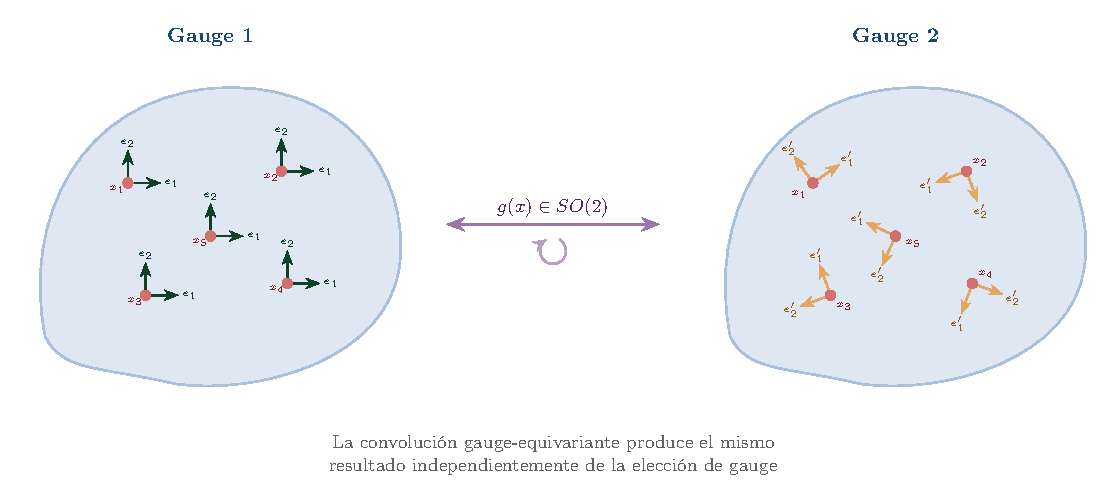
\includegraphics[width=0.90\textwidth]{images/gauge_freedom}
	\caption[Libertad gauge: elección de marcos locales]{Libertad gauge: la misma superficie admite diferentes elecciones de marcos locales (Gauge 1 y Gauge 2). La convolución gauge-equivariante produce resultados idénticos independientemente de la elección de gauge, conectados por transformaciones $g(x) \in SO(2)$ punto a punto.}
	\label{fig:gauge_freedom}
\end{figure}

\subsubsection{El problema de las simetrías rígidas}

Las CNNs clásicas asumen que las mismas transformaciones (traslaciones) son válidas en todo el dominio. Esta suposición funciona bien para imágenes planas, pero falla sistemáticamente cuando los datos tienen estructura geométrica intrínseca.

\begin{example}[Rotaciones en una Esfera]
Consideremos una imagen de la Tierra proyectada sobre una esfera. Si aplicamos una rotación global de $90^\circ$ alrededor del eje norte-sur:
\begin{itemize}
    \item En el ecuador, la rotación preserva perfectamente las formas locales
    \item Cerca de los polos, la misma rotación causa distorsión severa
    \item Una imagen de un continente cerca del polo norte se ve completamente diferente después de la rotación global
\end{itemize}
Este ejemplo ilustra que \textbf{la transformación apropiada depende de la posición}.
\end{example}

\textbf{Fracaso de la Equivarianza Global.} En espacios curvos o con topología no trivial, aplicar la misma transformación en todas partes puede:
\begin{enumerate}
    \item \textbf{Romper la estructura geométrica natural} del dominio
    \item \textbf{Introducir distorsiones artificiales} que no existían en los datos originales
    \item \textbf{Violar los principios físicos} que gobiernan el fenómeno modelado
\end{enumerate}

\subsubsection{Analogías físicas fundamentales}

La teoría gauge tiene sus raíces en la física, donde describe fenómenos donde la descripción matemática depende de elecciones arbitrarias de coordenadas o referencias locales.

\begin{example}[Electromagnetismo: El Paradigma Clásico]
En electromagnetismo, los campos físicos observables (como el campo eléctrico $\mathbf{E}$ y magnético $\mathbf{B}$) no dependen de cómo elegimos describir el potencial electromagnético $A_\mu(x)$. 

\textbf{Libertad Gauge}: Podemos transformar $A_\mu(x) \mapsto A_\mu(x) + \partial_\mu \Lambda(x)$ donde $\Lambda(x)$ es una función arbitraria que puede variar de punto a punto.

\textbf{Invariancia Física}: Los campos observables permanecen inalterados:
\begin{align}
\mathbf{E} &= -\nabla \phi - \frac{\partial \mathbf{A}}{\partial t} \\
\mathbf{B} &= \nabla \times \mathbf{A}
\end{align}
permanecen invariantes bajo la transformación gauge.

\textbf{Conexión con Deep Learning}: Al igual que las leyes físicas no deben depender de nuestra elección de coordenadas, las representaciones neuronales no deberían depender de elecciones arbitrarias de sistemas de referencia locales.
\end{example}

\begin{example}[Navegación en la Tierra: Sistemas de Coordenadas Locales]
Imagina que estás desarrollando un sistema de navegación global:
\begin{itemize}
    \item En Nueva York, es natural usar coordenadas que apunten hacia el "norte geográfico"
    \item En Sidney, el "norte geográfico" apunta en una dirección completamente diferente del espacio tridimensional
    \item No obstante, las \textit{relaciones locales} (izquierda, derecha, adelante, atrás) son consistentes en ambas ciudades
\end{itemize}

Una red neuronal \textbf{gauge equivariante} puede aprender a reconocer patrones que son invariantes a estas elecciones de sistema de coordenadas locales, mientras mantiene la capacidad de explotar la estructura geométrica real del problema.
\end{example}

\subsubsection{Progresión conceptual: de simple a complejo}

Para construir intuición, consideremos la progresión natural desde casos simples hacia la generalidad completa:

\begin{enumerate}
    \item \textbf{CNNs Clásicas}: Una sola transformación (traslación) válida globalmente
    \item \textbf{Group-CNNs}: Un conjunto finito de transformaciones válidas globalmente  
    \item \textbf{CNNs en Variedades}: Transformaciones dictadas por la geometría específica de la variedad
    \item \textbf{Gauge CNNs}: Libertad completa para elegir transformaciones locales, sujetas a consistencia
\end{enumerate}

\textbf{¿Por qué no simplemente data augmentation?} Alguien podría preguntar: "¿Por qué no simplemente aumentar los datos con múltiples transformaciones locales?" La respuesta es fundamental:

\begin{itemize}
    \item \textbf{Data augmentation}: Espera lograr invariancia \textit{estadísticamente} a través de múltiples muestras
    \item \textbf{Gauge equivariance}: Garantiza invariancia \textit{exacta} a través de la arquitectura
    \item \textbf{Eficiencia}: Gauge equivarianza logra con una sola forward pass lo que data augmentation requiere múltiples evaluaciones
    \item \textbf{Consistencia}: Garantiza que la red no pueda aprender a explotar transformaciones "accidentales" que no reflejan la verdadera estructura del problema
\end{itemize}

\subsection{Ejemplo Concreto: Gauge Equivarianza en Acción}\label{subsec:ejemplo_gauge_equivarianza}

Para hacer concretos estos conceptos abstractos, desarrollemos un ejemplo simple pero ilustrativo que muestra cómo funcionan las transformaciones gauge en la práctica.

\subsubsection{Escenario: Reconocimiento de patrones en una superficie cilíndrica}

Consideremos el problema de reconocer texturas en un cilindro (como un tronco de árbol). Los datos consisten en una imagen "envuelta" alrededor del cilindro.

\begin{example}[Problema de Coordenadas Locales en un Cilindro]
Supongamos que tenemos una textura de corteza de árbol fotografiada en diferentes posiciones alrededor del tronco:
\begin{itemize}
    \item \textbf{Posición A}: Foto tomada mirando hacia el norte
    \item \textbf{Posición B}: Foto tomada mirando hacia el este  
    \item \textbf{Posición C}: Foto tomada mirando hacia el sur
\end{itemize}

En cada posición, establecemos coordenadas locales $(u,v)$ donde:
\begin{itemize}
    \item $u$: dirección "horizontal" relativa a la orientación de la cámara
    \item $v$: dirección "vertical" (a lo largo del eje del tronco)
\end{itemize}

\textbf{El problema}: Los mismos patrones físicos de corteza se ven como tensores completamente diferentes en cada sistema de coordenadas locales.
\end{example}

\subsubsection{Solución gauge: transformaciones locales coherentes}

\begin{definition}[Transformación Gauge Simple]
Para nuestro cilindro, una \textbf{transformación gauge} es una función $g: S^1 \times \mathbb{R} \to SO(2)$ que asigna a cada punto $(\theta, z)$ del cilindro una rotación local en el plano tangente:
\begin{equation}
g(\theta, z) = \begin{pmatrix}
\cos(\phi(\theta, z)) & -\sin(\phi(\theta, z)) \\
\sin(\phi(\theta, z)) & \cos(\phi(\theta, z))
\end{pmatrix}
\end{equation}
donde $\phi(\theta, z)$ puede variar suavemente sobre la superficie.
\end{definition}

\begin{example}[Convolución Gauge en el Cilindro]\label{ex:convolucion_gauge_cilindro}
Una convolución gauge equivariante en este escenario sería:
\begin{equation}
[f \star \psi]_\text{gauge}(\theta, z) = \int_{N(\theta,z)} \psi\left(g(\theta', z')^{-1} \cdot \text{connect}((\theta,z), (\theta',z'))\right) f(\theta', z') \, d\theta' dz'
\end{equation}

donde:
\begin{itemize}
    \item $N(\theta,z)$ es un entorno del punto $(\theta,z)$
    \item $\text{connect}((\theta,z), (\theta',z'))$ describe cómo "conectar" los sistemas de coordenadas locales
    \item $\psi$ es un kernel que opera en el espacio de "diferencias de orientación"
\end{itemize}

\textbf{Propiedad clave}: Si aplicamos diferentes elecciones de orientación local $g(\theta,z)$ en cada punto, el resultado final de la convolución permanece invariante.
\end{example}

\subsubsection{Visualización del transporte de información}

\begin{figure}[htbp]
	\centering
	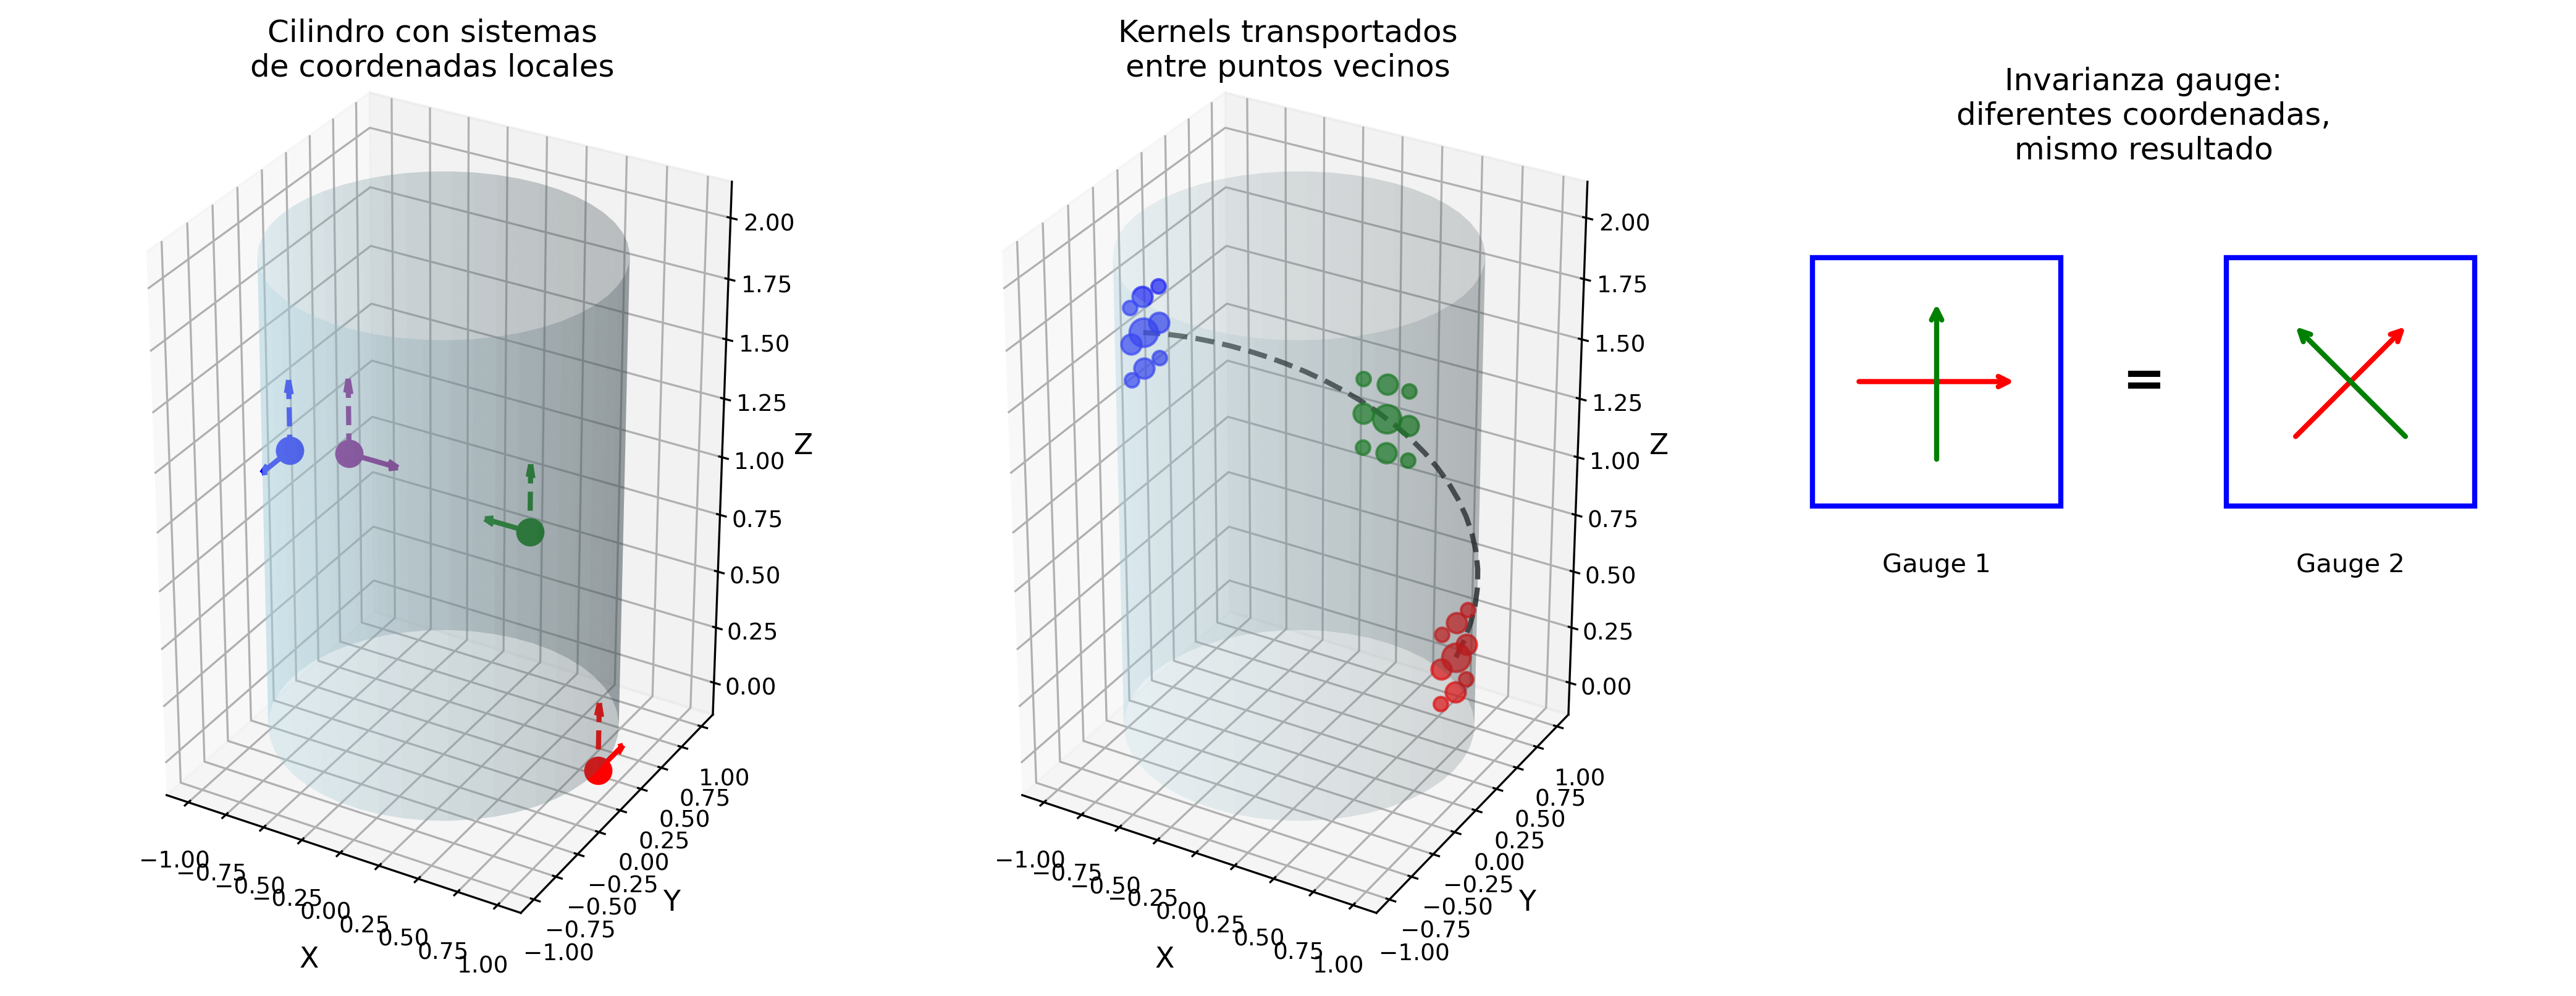
\includegraphics[width=0.95\textwidth]{images/gauge_transport_cylinder.png}
	\caption[Transporte gauge en un cilindro]{Transporte gauge en un cilindro. Izquierda: sistemas de coordenadas locales (vectores tangentes) en diferentes puntos del cilindro. Centro: kernels de convolución transportados a lo largo de una geodésica entre puntos vecinos. Derecha: concepto de invarianza gauge: diferentes elecciones de orientación local (Gauge 1 vs Gauge 2) producen el mismo patrón detectado.}
	\label{fig:gauge_transport_cylinder}
\end{figure}

\textbf{Intuición Clave: Separación de Forma y Orientación.} La gauge equivarianza permite que la red aprenda sobre:
\begin{itemize}
    \item \textbf{Forma intrínseca}: Qué patrones están presentes (independiente de orientación)
    \item \textbf{Relaciones espaciales}: Cómo los patrones se relacionan geométricamente
\end{itemize}
mientras ignora completamente:
\begin{itemize}
    \item \textbf{Orientación absoluta}: Elecciones arbitrarias de ``norte'', ``arriba'', etc.
    \item \textbf{Sistemas de coordenadas}: Convenciones de etiquetado que no afectan la física
\end{itemize}

\begin{proposition}[Gauge Equivarianza en el Cilindro]\label{prop:gauge_equivarianza_cilindro}
Sea $f: S^1 \times \mathbb{R} \to \mathbb{R}^d$ un campo de características sobre el cilindro y sea $g: S^1 \times \mathbb{R} \to SO(2)$ una transformación gauge arbitraria. La convolución gauge $[f \star \psi]_{\text{gauge}}$ definida en el \autoref{ex:convolucion_gauge_cilindro} satisface:
\begin{equation}
[(\rho(g) \cdot f) \star \psi]_{\text{gauge}} = \rho(g) \cdot [f \star \psi]_{\text{gauge}}
\end{equation}
donde $(\rho(g) \cdot f)(\theta, z) = g(\theta,z) \cdot f(\theta, z)$ es la acción gauge punto a punto.
\end{proposition}

\begin{proof}
Sustituyendo la definición:
\begin{align}
[(\rho(g) \cdot f) \star \psi]_{\text{gauge}}(\theta, z) &= \int_{N(\theta,z)} \psi\left(g(\theta',z')^{-1} \cdot c_{(\theta,z) \to (\theta',z')}\right) g(\theta',z') f(\theta',z') \, d\theta' dz'
\end{align}
donde $c_{(\theta,z) \to (\theta',z')}$ denota la conexión (transporte paralelo) entre los marcos locales. Como $g(\theta',z')^{-1} g(\theta',z') = \operatorname{Id}$, la transformación gauge en el campo $f$ se cancela con la transformación inversa en el argumento de $\psi$, dejando el resultado transformado por $g(\theta,z)$ en el punto de salida.
\end{proof}

\begin{remark}[Analogía con Teorías Gauge en Física]
La estructura matemática de esta proposición es idéntica a la de las teorías gauge en física de partículas. En electrodinámica, el potencial vector $A_\mu$ (análogo a nuestro campo $f$) se transforma bajo un cambio gauge $A_\mu \to A_\mu + \partial_\mu \chi$, pero el tensor de campo $F_{\mu\nu} = \partial_\mu A_\nu - \partial_\nu A_\mu$ (análogo a la salida de la convolución) es gauge-invariante. La convolución gauge de Cohen et al. implementa exactamente este principio en el contexto de redes neuronales.
\end{remark}

\subsection{Fundamentos Matemáticos de la Teoría Gauge}\label{subsec:fundamentos_matematicos_gauge}

La distinción fundamental entre simetrías globales y locales se formaliza de la siguiente manera:

\begin{definition}[Transformación Local vs. Global]
Para un grupo $G$ y función $f: \mathcal{M} \to \mathbb{R}^d$:

\textbf{Transformación Global}: $T_g[f](x) = \rho(g) f(g^{-1} \cdot x)$, donde $g \in G$ es el mismo elemento para todos los puntos $x \in \mathcal{M}$.

\textbf{Transformación Local (Gauge)}: $T_{g(\cdot)}[f](x) = \rho(g(x)) f(\phi_{g(x)}(x))$, donde $g: \mathcal{M} \to G$ asigna a cada punto $x$ una transformación $g(x) \in G$.
\end{definition}

La libertad de elegir transformaciones locales independientes plantea un problema fundamental: ¿cómo comparar información entre puntos con sistemas de coordenadas distintos? La respuesta proviene de la teoría de fibrados principales (\autoref{def:fibrado_principal_formal}, \autoref{ch:gdl}), que asocia a cada punto del espacio todas sus posibles orientaciones locales. En nuestro ejemplo del cilindro, el fibrado es $P = (S^1 \times \mathbb{R}) \times SO(2)$, donde cada punto $(\theta, z, R) \in P$ representa una posición con orientación local $R$.

Las \textbf{conexiones} (\autoref{def:conexion_fibrado}) resuelven el problema de comparación especificando cómo transportar orientaciones entre puntos vecinos de manera consistente, y el \textbf{transporte paralelo} (\autoref{def:transporte_paralelo_formal}) permite comparar objetos en diferentes fibras. Para una exposición completa de este formalismo, véase la \autoref{sec:gauges_invarianzas}.

\begin{proposition}[Obstrucción Topológica a Gauges Globales]\label{prop:obstruccion_gauge_global}
Sea $\mathcal{M}$ una variedad diferenciable y $P \to \mathcal{M}$ un fibrado principal con grupo de estructura $G$. El fibrado admite una sección global (es decir, una elección consistente de gauge en toda $\mathcal{M}$) si y solo si $P$ es trivial ($P \cong \mathcal{M} \times G$). En particular:
\begin{enumerate}
    \item El fibrado de marcos de $S^2$ no admite sección global (por el teorema de la bola peluda).
    \item Todo fibrado principal sobre una variedad contráctil es trivial.
\end{enumerate}
\end{proposition}

\begin{proof}
Una sección global $s: \mathcal{M} \to P$ induce la trivialización $\mathcal{M} \times G \to P$ dada por $(x, g) \mapsto s(x) \cdot g$, que es un isomorfismo de fibrados por la acción libre y transitiva de $G$ en cada fibra. Recíprocamente, una trivialización $P \cong \mathcal{M} \times G$ proporciona la sección $s(x) = (x, e)$.

Para (1), una sección del fibrado de marcos ortonormales $\operatorname{SO}(\mathcal{M})$ de $S^2$ equivale a un campo de bases ortonormales continuo, lo que implica en particular un campo vectorial tangente que no se anula, contradiciendo el teorema de la bola peluda (la característica de Euler $\chi(S^2) = 2 \neq 0$).

Para (2), toda variedad contráctil es homotópicamente equivalente a un punto, luego todo fibrado principal sobre ella es trivial (ya que los fibrados se clasifican por clases de homotopía de mapas al espacio clasificante $BG$).
\end{proof}

\begin{remark}[Implicación para Redes Neuronales]
La \autoref{prop:obstruccion_gauge_global} explica por qué la gauge equivarianza es \textit{necesaria} (no solo conveniente) para redes neuronales en superficies generales: en la esfera $S^2$ y en la mayoría de variedades de interés, no existe un sistema de coordenadas global consistente. Cualquier parametrización global tiene singularidades (como los polos en coordenadas esféricas). La gauge equivarianza permite que la red sea independiente de estas elecciones locales, evitando artefactos en las singularidades.
\end{remark}

\subsubsection{Hacia la implementación práctica}

La brecha entre la teoría (fibrados infinitamente dimensionales con conexiones suaves) y la práctica (redes neuronales discretas con parámetros finitos) es significativa. El trabajo pionero de Cohen et al.\ mostró cómo encontrar discretizaciones que preserven las propiedades teóricas esenciales. La clave reside en que la gauge equivarianza impone restricciones \textit{lineales} sobre los pesos de la red, reduciendo el espacio de parámetros a un subespacio afín que puede resolverse analíticamente antes del entrenamiento.

\subsection{Gauge Equivariant CNNs: El Modelo de Cohen et al.}\label{subsec:modelo_cohen_gauge}

El trabajo seminal de Cohen et al.~\citep{cohen2019gaugeequivariantconvolutional} representa el primer éxito en traducir la teoría gauge abstracta a una arquitectura neuronal práctica y eficiente. Su contribución clave fue mostrar cómo implementar gauge equivarianza exacta mientras manteniendo la estructura básica de las convoluciones.

\subsubsection{Filosofía del diseño: de lo abstracto a lo concreto}

La aproximación de Cohen et al. sigue una filosofía de diseño clara:
\begin{enumerate}
    \item \textbf{Principio}: Identificar las propiedades geométricas fundamentales que debe preservar la arquitectura
    \item \textbf{Discretización}: Encontrar una representación finita que capture estas propiedades  
    \item \textbf{Implementación}: Traducir a operaciones que puedan ejecutarse eficientemente
    \item \textbf{Verificación}: Demostrar que la implementación respeta las propiedades teóricas
\end{enumerate}

Los conceptos de curvatura (\autoref{def:curvatura_formal}) y transporte paralelo (\autoref{def:transporte_paralelo_formal}), fundamentales para la construcción de convoluciones gauge equivariantes, se desarrollan formalmente en la \autoref{sec:gauges_invarianzas}. La curvatura mide el ``defecto de integrabilidad'' de la conexión (cuánto depende el transporte paralelo del camino elegido), mientras que el transporte paralelo proporciona el mecanismo para comparar elementos en fibras diferentes.

\subsubsection{El caso específico: icosahedral CNNs}

Para hacer concretas estas ideas abstractas, Cohen et al. se enfocan en un caso específico que combina riqueza teórica con viabilidad computacional.

\begin{example}[¿Por qué el Icosaedro?]
La elección del icosaedro como dominio no es arbitraria:

\textbf{Propiedades geométricas}:
\begin{itemize}
    \item \textbf{Mejor aproximación esférica}: Entre los poliedros regulares, es el que mejor aproxima la esfera
    \item \textbf{Simetría rica}: Grupo de simetría $I_h$ con 120 elementos
    \item \textbf{Regularidad geodésica}: Distancias entre vértices aproximadamente uniformes
    \item \textbf{Triangulación canónica}: Estructura de malla bien definida
\end{itemize}

\textbf{Propiedades computacionales}:
\begin{itemize}
    \item \textbf{Tamaño manejable}: 12 vértices, 20 caras, 30 aristas
    \item \textbf{Subdivisión sistemática}: Refinamiento por subdivisión geodésica
    \item \textbf{Coordenadas baricéntricas}: Interpolación suave en cada cara triangular
    \item \textbf{Implementación eficiente}: Estructura de datos optimizada
\end{itemize}
\end{example}

\begin{definition}[Discretización Icosaédrica]\label{def:discretizacion_icosaedrica}
La discretización icosaédrica de la esfera $S^2$ se obtiene mediante:

\textbf{Construcción geométrica}:
\begin{enumerate}
    \item \textbf{Icosaedro inscrito}: 12 vértices ubicados en $S^2$ con simetría máxima
    \item \textbf{Proyección radial}: Cada punto de la esfera se asigna al vértice más cercano
    \item \textbf{Refinamiento geodésico}: Subdivisión de aristas por grandes círculos
\end{enumerate}

\textbf{Parametrización}: Cada punto en $S^2$ se representa como:
\begin{equation}
p = \sum_{i=1}^{12} w_i v_i, \quad \sum_{i=1}^{12} w_i = 1, \quad w_i \geq 0
\end{equation}
donde $\{v_i\}$ son los vértices icosaédricos y $\{w_i\}$ son coordenadas baricéntricas.
\end{definition}

\begin{definition}[Transformación Gauge Local]\label{def:transformacion_gauge_local}
En la discretización icosaédrica, las transformaciones gauge locales se definen como:
\begin{equation}
h: S^2 \to SO(2)
\end{equation}
donde $h(p) \in SO(2)$ especifica la transformación en el punto $p$.

\textbf{Restricción de regularidad}: Para garantizar diferenciabilidad, se requiere:
\begin{equation}
\|h(p) - h(q)\| \leq C d(p,q)^\alpha
\end{equation}
para alguna constante $C$ y exponente Hölder $\alpha \in (0,1]$.
\end{definition}

\begin{definition}[Función Gauge Equivariante]\label{def:funcion_gauge_equivariante}
Una función $f: S^2 \to \mathbb{R}^n$ se dice gauge equivariante si para toda transformación gauge $h$:
\begin{equation}
f^h(p) = \rho(h(p)^{-1}) f(p)
\end{equation}
donde $\rho: SO(2) \to GL(\mathbb{R}^n)$ es una representación del grupo.

\textbf{Casos especiales importantes}:
\begin{itemize}
    \item \textbf{Escalares} ($n=1$): $\rho$ trivial, $f^h = f$
    \item \textbf{Vectores} ($n=2$): $\rho$ es la representación estándar de $SO(2)$
    \item \textbf{Campos complejos}: Multiplicación por $e^{i\theta}$ para rotación por ángulo $\theta$
\end{itemize}
\end{definition}

\begin{theorem}[Convolución Gauge Equivariante]\label{thm:convolucion_gauge_equivariante}
Para funciones gauge equivariantes $f, g: S^2 \to \mathbb{R}^n$, su convolución gauge se define como:
\begin{equation}
(f *_G g)(p) = \int_{S^2} f(q) \cdot G(q, p) \cdot g(q) \, d\sigma(q)
\end{equation}
donde $G(q,p)$ es el propagador gauge que codifica el transporte paralelo de $q$ a $p$.

Si $f$ y $g$ son gauge equivariantes, entonces $f *_G g$ también es gauge equivariante.
\end{theorem}

\begin{proof}
Sea $\rho_p$ un cambio de gauge en el punto $p$ (un cambio de base local del espacio tangente), de modo que las funciones gauge equivariantes se transforman como $f(p) \mapsto \rho_p \cdot f(p)$. El propagador gauge $G(q,p)$ codifica el transporte paralelo de $q$ a $p$ y transforma como $G(q,p) \mapsto \rho_p \cdot G(q,p) \cdot \rho_q^{-1}$ (pues cambia de la base en $q$ a la base en $p$). Entonces:
\begin{align}
(f *_G g)(p) &\mapsto \int_{S^2} (\rho_q f(q)) \cdot (\rho_p G(q,p) \rho_q^{-1}) \cdot (\rho_q g(q)) \, d\sigma(q) \\
&= \rho_p \int_{S^2} f(q) \cdot G(q,p) \cdot g(q) \, d\sigma(q) = \rho_p \cdot (f *_G g)(p)
\end{align}
donde usamos que $\rho_q^{-1} \rho_q = \operatorname{Id}$. Así, $f *_G g$ se transforma como $\rho_p \cdot (f *_G g)(p)$, que es la ley de transformación gauge equivariante.
\end{proof}

\textbf{Implementación del propagador gauge}: En la práctica, $G(q,p)$ se implementa mediante:

\begin{algorithm}[H]
\caption{Cálculo del Propagador Gauge Icosaédrico}
\begin{algorithmic}[1]
    \State \textbf{Entrada:} Puntos $q, p \in S^2$, conexión gauge $\omega$
    \State Encontrar camino geodésico $\gamma: q \to p$ en la discretización
    \State Inicializar elemento de grupo $g = I \in SO(2)$
    \For{cada arista $e$ en el camino $\gamma$}
        \State Actualizar: $g \leftarrow g \cdot \exp(-\omega_e)$
    \EndFor
    \State \textbf{Salida:} $G(q,p) = g$
\end{algorithmic}
\end{algorithm}

\subsubsection{Construcción teórica simplificada}

\begin{theorem}[Construcción Simplificada de Gauge CNNs]
Para hacer las ideas más accesibles, presentamos una construcción simplificada que mantiene los elementos esenciales:

\textbf{Datos de entrada}: Una función $f: V \to \mathbb{R}^d$ definida en los vértices icosaédricos $V = \{v_1, \ldots, v_{12}\}$.

\textbf{Convolución gauge local}: En cada vértice $v_i$:
\begin{equation}
(f * \psi)(v_i) = \sum_{j \in \mathcal{N}(i)} \psi_{ij} \cdot \Gamma_{ij} \cdot f(v_j)
\end{equation}
donde:
\begin{itemize}
    \item $\mathcal{N}(i)$ son los vértices vecinos de $v_i$
    \item $\psi_{ij}$ son pesos de kernel aprendibles
    \item $\Gamma_{ij} \in SO(2)$ es el transporte gauge de $v_j$ a $v_i$
\end{itemize}

\textbf{Aprendizaje de la conexión}: Los elementos de transporte $\Gamma_{ij}$ se parametrizan como:
\begin{equation}
\Gamma_{ij} = \exp(i\theta_{ij}), \quad \theta_{ij} \in [0, 2\pi)
\end{equation}
y los ángulos $\{\theta_{ij}\}$ son parámetros aprendibles de la red.

\textbf{Regularización gauge}: Para evitar soluciones degeneradas, se añade un término de regularización:
\begin{equation}
\mathcal{R}(\theta) = \sum_{\text{triángulos } T} \left|\sum_{(i,j) \in \partial T} \theta_{ij}\right|^2
\end{equation}
que penaliza curvatura excesiva (holonomía no trivial en triángulos pequeños). Esta regularización es una consecuencia práctica de la identidad de Bianchi~\eqref{eq:bianchi}.
\end{theorem}

\subsection{Marco General de Fibrados Principales}

Más allá del ejemplo icosaédrico, la teoría gauge proporciona un marco general para el diseño de arquitecturas neuronales equivariantes en contextos geométricos complejos.

\subsubsection{Clasificación de estructuras gauge}

Diferentes problemas requieren diferentes elecciones de fibrado principal, determinadas por las simetrías intrínsecas de los datos.

\begin{theorem}[Clasificación de Fibrados para Deep Learning]
Sea $\mathcal{M}$ una variedad que modela el dominio de los datos y $G$ el grupo de simetrías relevantes. Los fibrados principales apropiados para arquitecturas gauge equivariantes se clasifican según:

\begin{enumerate}
\item \textbf{Fibrados triviales}: $P = \mathcal{M} \times G$ cuando las simetrías son globalmente consistentes
\item \textbf{Fibrados de frames}: Cuando se requiere invariancia bajo cambios de coordenadas locales
\item \textbf{Fibrados de spin}: Para datos con estructura de orientación (común en física de partículas)
\item \textbf{Fibrados gauge}: Para campos con simetrías internas (electromagnetismo, campos de Yang-Mills)
\end{enumerate}
\end{theorem}

\subsubsection{Propiedades de aproximación universal}

La formulación rigorosa de convoluciones gauge equivariantes utiliza el transporte paralelo (\autoref{def:transporte_paralelo_formal}) para comparar fibras en diferentes puntos de la variedad base, preservando la estructura gauge.

Un resultado teórico fundamental establece que las redes gauge equivariantes poseen propiedades de aproximación universal en contextos apropiados.

\begin{theorem}[Aproximación Universal Gauge]
Sea $\mathcal{F}_{\text{gauge}}$ el espacio de funciones implementables por redes gauge equivariantes con profundidad y anchura suficientes. Entonces:

\begin{enumerate}
\item $\mathcal{F}_{\text{gauge}}$ es denso en $L^2_{\text{gauge}}(P)$, el espacio de funciones gauge equivariantes de cuadrado integrable
\item La tasa de aproximación es $O(n^{-2/(d_{\mathcal{M}} + d_G)})$ donde $d_{\mathcal{M}}$ es la dimensión de la variedad base y $d_G$ la dimensión del grupo gauge
\item Las constantes de aproximación dependen únicamente de la curvatura del fibrado y las propiedades de regularidad de la conexión
\end{enumerate}

Véase la Sección~\ref{sec:aproximacion_universal_gauge} del \autoref{ch:teoremas_complementarios} para el esbozo de demostración.
\end{theorem}

\subsection{Fundamentos Matemáticos Profundos}

Los fundamentos matemáticos de la teoría gauge (incluyendo la curvatura de conexión (\autoref{def:curvatura_formal}), la ecuación de estructura de Cartan (\autoref{thm:cartan_estructura}) y la holonomía (\autoref{def:holonomia})) se desarrollan formalmente en la \autoref{sec:gauges_invarianzas} del \autoref{ch:gdl}. Aquí nos enfocamos en las aplicaciones de estos conceptos a la geometría y la física.

\subsubsection{Aplicaciones matemáticas en geometría y física}

La teoría de convoluciones gauge proporciona marcos unificadores para modelar fenómenos donde las simetrías locales desempeñan un papel fundamental.

\paragraph{Teorías de campo gauge}
Los campos gauge fundamentales de la física teórica se modelan naturalmente mediante fibrados principales con grupos de estructura específicos.

\begin{example}[Electrodinámica Cuántica]
El electromagnetismo se describe mediante el fibrado principal $(P, \mathcal{M}, \pi, U(1))$ donde:
\begin{itemize}
\item La variedad base $\mathcal{M}$ representa el espaciotiempo
\item El grupo $U(1)$ codifica las transformaciones de fase electromagnética
\item La conexión $A$ es el potencial vectorial electromagnético
\item La curvatura $F = dA$ es el tensor de campo electromagnético
\end{itemize}
\end{example}

\paragraph{Geometría diferencial}
Las estructuras gauge aparecen naturalmente en el estudio de variedades riemannianas y sus generalizaciones.

\begin{example}[Fibrado de Frames Ortogonales]
Para una variedad riemanniana $(\mathcal{M}, g)$, el fibrado de frames ortonormales $O(\mathcal{M})$ es un fibrado principal con grupo estructural $O(n)$. Las convoluciones gauge en este contexto respetan las isometrías locales de la métrica riemanniana.
\end{example}

\paragraph{Topología algebraica}
Las clases características de fibrados principales proporcionan invariantes topológicos que clasifican completamente las estructuras gauge hasta isomorfismo.

\begin{example}[Clases de Chern]
Para fibrados complejos, las clases de Chern $c_k \in H^{2k}(\mathcal{M}, \mathbb{Z})$ proporcionan obstrucciones topológicas para la existencia de secciones globales y conexiones con curvatura prescrita.
\end{example}

\subsection{Extensiones Teóricas y Desarrollos Recientes}

\subsubsection{Gauge CNNs en dimensiones superiores}

Las extensiones de la teoría gauge a dimensiones superiores y estructuras más complejas representan un área activa de investigación.

\begin{definition}[Fibrado Principal de Orden Superior]
Un \textbf{fibrado principal de orden superior} es una secuencia de fibrados:
\begin{equation}
G \to P_n \to P_{n-1} \to \cdots \to P_1 \to \mathcal{M}
\end{equation}
donde cada nivel introduce simetrías adicionales. Estas estructuras modelan sistemas físicos con múltiples escalas de simetría.
\end{definition}

\paragraph{Aplicaciones en teorías de campo unificadas}
Las teorías de gauge no abelianas (como la cromodinámica cuántica) requieren fibrados principales con grupos no conmutativos:

\begin{example}[QCD Lattice]
La cromodinámica cuántica en red se modela mediante:
\begin{itemize}
\item Variedad base: Red espaciotemporal discreta
\item Grupo gauge: $SU(3)$ (grupo de color)
\item Campos: Conexiones gauge en enlaces de la red
\item Estructura gauge: Describe las interacciones fundamentales entre quarks y gluones
\end{itemize}
\end{example}

\subsubsection{Conexión con álgebras de Lie generalizadas}

Desarrollos recientes exploran la conexión entre gauge CNNs y estructuras algebraicas más generales.

\begin{theorem}[Representación por Álgebras de Lie]
Toda gauge CNN puede representarse mediante un álgebra de Lie generalizada $\mathfrak{L}$ que actúa en el espacio de características. La estructura de $\mathfrak{L}$ determina completamente las propiedades de equivarianza de la red.
\end{theorem}

Esta representación permite:
\begin{itemize}
\item Clasificación sistemática de estructuras gauge mediante invariantes algebraicos
\item Caracterización completa de propiedades de equivarianza vía teoría de representaciones
\item Análisis geométrico de espacios de modulación gauge
\end{itemize}

\subsubsection{Gauge CNNs cuánticas}

Una frontera emergente explora la extensión de principios gauge al dominio de la computación cuántica.

\begin{definition}[Gauge CNN Cuántica]
Una \textbf{gauge CNN cuántica} es un circuito cuántico parametrizado que preserva simetrías gauge mediante operaciones unitarias:
\begin{equation}
U_{\text{gauge}}(\theta) = \exp\left(i \sum_j \theta_j H_j^{\text{gauge}}\right)
\end{equation}
donde los $H_j^{\text{gauge}}$ son hamiltonianos que conmutan con generadores gauge.
\end{definition}

Las aplicaciones potenciales incluyen:
\begin{itemize}
\item Simulación de sistemas gauge cuánticos
\item Procesamiento de datos en espacios de Hilbert curvos
\item Algoritmos cuánticos para problemas de optimización con simetrías
\end{itemize}

\subsubsection{Perspectivas futuras}

El desarrollo de convoluciones gauge representa solo el inicio de una revolución conceptual en el aprendizaje profundo geométrico. Las direcciones prometedoras incluyen:

\paragraph{Teoría de gauge adaptativa}
Desarrollo de métodos variacionales para la determinación óptima de estructuras de fibrado mediante principios de mínima acción generalizada, extendiendo el formalismo lagrangiano clásico.

\paragraph{Renormalización geométrica}
Integración de técnicas de renormalización diferencial para el tratamiento sistemático de singularidades gauge en múltiples escalas geométricas.

\paragraph{Extensiones a geometrías no commutativas}
Generalización del formalismo gauge a variedades no conmutativas, donde la estructura del fibrado principal se reemplaza por módulos proyectivos sobre álgebras de operadores.

La teoría gauge, importada de la física fundamental al aprendizaje automático, promete establecer principios unificadores para el diseño de arquitecturas neuronales que respeten las simetrías profundas inherentes en la estructura de nuestro universo físico y matemático.

\section{Extensiones Algebraicas Avanzadas}\label{sec:algebraic_extensions}

Después de explorar las convoluciones gauge, que proporcionan un marco elegante para manejar simetrías locales, nos adentramos en territorios aún más abstractos y poderosos. Las extensiones algebraicas avanzadas representan las fronteras más innovadoras del \gls{GDL}, donde estructuras matemáticas sofisticadas como las álgebras de Clifford y los métodos topológicos abren nuevas posibilidades para el procesamiento de datos geométricos.

Estas extensiones no solo amplían la expresividad de las arquitecturas existentes, sino que revelan conexiones profundas entre el álgebra abstracta, la topología algebraica y el aprendizaje automático. Su importancia radica en proporcionar marcos unificadores que pueden manejar una variedad mucho más amplia de datos geométricos y estructurales de lo que era posible anteriormente.

\subsection{Álgebras de Clifford y Geométricas}

Las álgebras de Clifford, también conocidas como álgebras geométricas, constituyen un marco algebraico unificado que generaliza números complejos, cuaterniones y otros sistemas numéricos avanzados. Su poder radica en la capacidad de representar transformaciones geométricas, rotaciones y reflexiones de manera natural y computacionalmente eficiente.

En el contexto de CNNs, las álgebras de Clifford permiten extender las convoluciones a dominios donde las transformaciones geométricas son inherentemente más complejas que las simples traslaciones euclidianas. A diferencia del tratamiento completo de álgebras de Clifford en el \autoref{ch:attention} (\autoref{sec:clifford_attention}), donde se estudian en el contexto de mecanismos de atención, aquí nos enfocamos en su aplicación específica a operaciones convolucionales y su conexión con estructuras topológicas.

\subsubsection{Fundamentos de Álgebras Geométricas}

\begin{definition}[Álgebra de Clifford]\label{def:clifford_cnn}
Sea $V$ un espacio vectorial de dimensión finita sobre $\mathbb{R}$ equipado con una forma cuadrática $Q$. El \textbf{álgebra de Clifford} $\text{Cl}(V,Q)$ es el álgebra asociativa unitaria generada por $V$ sujeta a la relación:
\[v^2 = Q(v) \cdot 1\]
para todo $v \in V$.
\end{definition}

En el contexto de \gls{GDL}, trabajamos típicamente con álgebras de Clifford definidas por una métrica con signatura $(p,q)$, denotada $\text{Cl}(p,q)$, donde $p$ dimensiones tienen norma positiva y $q$ dimensiones tienen norma negativa.

\textbf{Relación con Estructuras Conocidas.}\label{rem:clifford_structures} Las álgebras de Clifford unifican varias estructuras algebraicas familiares:
\begin{itemize}
    \item $\text{Cl}(0,0) \cong \mathbb{R}$ (números reales)
    \item $\text{Cl}(0,1) \cong \mathbb{C}$ (números complejos)
    \item $\text{Cl}(0,2) \cong \mathbb{H}$ (cuaterniones de Hamilton; véase Sección~\ref{sec:cuaterniones} del Apéndice~\ref{ch:teoremas_complementarios} para sus propiedades y su relación con $SU(2)$)
    \item $\text{Cl}(3,0) \cong \mathbb{R}^{8}$ (álgebra geométrica euclidiana 3D)
\end{itemize}

\textbf{Elementos Fundamentales y Gradación:}

\begin{definition}[Multivector y Gradación]\label{def:multivector_cnn}
Los elementos del álgebra de Clifford se llaman \textit{multivectores} y admiten una descomposición única por grados. Para $\text{Cl}(p,q)$ con $n = p+q$:
\[M = \langle M \rangle_0 + \langle M \rangle_1 + \langle M \rangle_2 + \cdots + \langle M \rangle_n\]
donde:
\begin{itemize}
    \item $\langle M \rangle_0 \in \mathbb{R}$: escalar
    \item $\langle M \rangle_1 \in \text{span}\{\mathbf{e}_1, \ldots, \mathbf{e}_n\}$: vector
    \item $\langle M \rangle_2 \in \text{span}\{\mathbf{e}_i \wedge \mathbf{e}_j : i < j\}$: bivector
    \item $\langle M \rangle_k$: $k$-vector con $\binom{n}{k}$ dimensiones
    \item $\langle M \rangle_n$: pseudoescalar
\end{itemize}
\end{definition}

\begin{theorem}[Dimensionalidad del Álgebra]\label{thm:dim_clifford_cnn}
El álgebra de Clifford $\text{Cl}(p,q)$ es un espacio vectorial de dimensión $2^{p+q}$, con base canónica formada por todos los productos wedge de subconjuntos de $\{\mathbf{e}_1, \ldots, \mathbf{e}_{p+q}\}$:
\[\dim(\text{Cl}(p,q)) = \sum_{k=0}^{p+q} \binom{p+q}{k} = 2^{p+q}\]
\end{theorem}

\begin{proof}
Sea $n = p + q$ y $\{\mathbf{e}_1, \ldots, \mathbf{e}_n\}$ la base ortonormal de $V$. Los elementos base del álgebra de Clifford son los productos ordenados $\mathbf{e}_{i_1} \mathbf{e}_{i_2} \cdots \mathbf{e}_{i_k}$ con $1 \leq i_1 < i_2 < \cdots < i_k \leq n$ y $0 \leq k \leq n$ (con la convención de que $k = 0$ corresponde al escalar $1$). Estos elementos son linealmente independientes, pues las relaciones $\mathbf{e}_i \mathbf{e}_j = -\mathbf{e}_j \mathbf{e}_i$ para $i \neq j$ permiten ordenar todo producto, y las relaciones $\mathbf{e}_i^2 = \pm 1$ eliminan cuadrados. El número de subconjuntos de $\{1, \ldots, n\}$ es $\sum_{k=0}^{n} \binom{n}{k} = 2^n$, que es la dimensión del álgebra.
\end{proof}

\textbf{Producto Geométrico:}

El concepto central del álgebra de Clifford es el \textit{producto geométrico}, que unifica el producto interior y el producto exterior.

\begin{definition}[Producto Geométrico]\label{def:producto_geometrico_cnn}
Para vectores $\mathbf{u}, \mathbf{v} \in V$, el \textbf{producto geométrico} se define como:
\[\mathbf{u}\mathbf{v} = \mathbf{u} \cdot \mathbf{v} + \mathbf{u} \wedge \mathbf{v}\]
donde:
\begin{itemize}
    \item $\mathbf{u} \cdot \mathbf{v} = \frac{1}{2}(\mathbf{u}\mathbf{v} + \mathbf{v}\mathbf{u})$ (producto interior, escalar)
    \item $\mathbf{u} \wedge \mathbf{v} = \frac{1}{2}(\mathbf{u}\mathbf{v} - \mathbf{v}\mathbf{u})$ (producto exterior, bivector)
\end{itemize}
\end{definition}

\begin{example}[Productos en $\text{Cl}(3,0)$]\label{ex:productos_cl30}
Consideremos el álgebra euclidiana tridimensional $\text{Cl}(3,0)$ con base $\{\mathbf{e}_1, \mathbf{e}_2, \mathbf{e}_3\}$ donde $\mathbf{e}_i^2 = 1$.

\textbf{Productos de base:}
\begin{align}
\mathbf{e}_1 \mathbf{e}_1 &= 1 \quad \text{(cuadrados dan escalar)} \\
\mathbf{e}_1 \mathbf{e}_2 &= \mathbf{e}_1 \wedge \mathbf{e}_2 \quad \text{(vectores ortogonales)} \\
\mathbf{e}_2 \mathbf{e}_1 &= -\mathbf{e}_1 \wedge \mathbf{e}_2 = -\mathbf{e}_1 \mathbf{e}_2
\end{align}

\textbf{Producto de bivector con vector:}
\[(\mathbf{e}_1 \wedge \mathbf{e}_2) \mathbf{e}_3 = \mathbf{e}_1 \mathbf{e}_2 \mathbf{e}_3 = \mathbf{e}_1 \wedge \mathbf{e}_2 \wedge \mathbf{e}_3\]
Este es el pseudoescalar unitario $I$ en $\text{Cl}(3,0)$.

\textbf{Bivector al cuadrado:}
\[(\mathbf{e}_1 \wedge \mathbf{e}_2)^2 = \mathbf{e}_1 \mathbf{e}_2 \mathbf{e}_1 \mathbf{e}_2 = -\mathbf{e}_1 \mathbf{e}_1 \mathbf{e}_2 \mathbf{e}_2 = -1\]
Los bivectores se comportan como números imaginarios.
\end{example}

\begin{example}[Rotores en 2D]\label{ex:rotores_2d}
En $\text{Cl}(2,0)$, un rotor que representa rotación por ángulo $\theta$ es:
\[R = \cos(\theta/2) + \sin(\theta/2) \mathbf{e}_1 \wedge \mathbf{e}_2 = e^{(\theta/2) \mathbf{e}_1 \wedge \mathbf{e}_2}\]

Para rotar un vector $\mathbf{v}$:
\[\mathbf{v}' = R \mathbf{v} \widetilde{R}\]
donde $\widetilde{R}$ es el reverso de $R$ (invierte orden de multiplicación en productos wedge).

\textbf{Verificación explícita para $\theta = \pi/2$:}
\[R = \frac{1}{\sqrt{2}}(1 + \mathbf{e}_1 \wedge \mathbf{e}_2), \quad \widetilde{R} = \frac{1}{\sqrt{2}}(1 - \mathbf{e}_1 \wedge \mathbf{e}_2)\]
\[R \mathbf{e}_1 \widetilde{R} = \frac{1}{2}(1 + \mathbf{e}_1 \mathbf{e}_2) \mathbf{e}_1 (1 - \mathbf{e}_1 \mathbf{e}_2) = \mathbf{e}_2\]
\end{example}

\begin{example}[Reflexiones]\label{ex:reflexiones_clifford}
La reflexión de un vector $\mathbf{v}$ respecto a un hiperplano perpendicular a $\mathbf{n}$ (unitario) es:
\[\mathbf{v}' = -\mathbf{n} \mathbf{v} \mathbf{n}\]

Para $\mathbf{n} = \mathbf{e}_1$ y $\mathbf{v} = a\mathbf{e}_1 + b\mathbf{e}_2$:
\[\mathbf{v}' = -\mathbf{e}_1 (a\mathbf{e}_1 + b\mathbf{e}_2) \mathbf{e}_1 = -a\mathbf{e}_1 + b\mathbf{e}_2\]
Como esperado, invierte la componente perpendicular al plano.
\end{example}

\subsubsection{Convoluciones en Álgebras de Clifford}

Aunque GATr se explora extensamente en el \autoref{ch:attention} (\autoref{sec:clifford_attention}), aquí examinamos cómo las álgebras de Clifford permiten definir operaciones convolucionales en dominios geométricos complejos.

\begin{definition}[Convolución Clifford-valuada]\label{def:conv_clifford}
Sea $f: \Omega \to \text{Cl}(p,q)$ una señal valuada en el álgebra de Clifford y $\psi: G \to \text{Cl}(p,q)$ un kernel definido sobre un grupo de transformaciones $G$. La \textbf{convolución Clifford-valuada} es:
\[(f \star \psi)(x) = \int_G \rho_g^{-1}(\psi(g)) \cdot f(g^{-1} \cdot x) \, dg\]
donde $\rho_g$ es la acción del grupo en el álgebra y $\cdot$ es el producto geométrico.
\end{definition}

\textbf{Ventajas sobre Convoluciones Escalares.}\label{rem:ventajas_clifford_conv} Las convoluciones Clifford-valuadas ofrecen:
\begin{enumerate}
    \item \textbf{Representación rica}: Los multivectores codifican múltiples aspectos geométricos simultáneamente
    \item \textbf{Equivarianza automática}: La estructura algebraica garantiza propiedades de simetría
    \item \textbf{Eficiencia computacional}: Operaciones de bajo nivel optimizables con SIMD
    \item \textbf{Interpretabilidad}: Los grados del multivector tienen significado geométrico claro
\end{enumerate}

\begin{example}[CNN Steerable con Clifford Algebra]\label{ex:steerable_clifford}
Consideremos una CNN 2D equivariante a rotaciones usando $\text{Cl}(2,0)$.

\textbf{Representación de características:}
Una característica en posición $\mathbf{x}$ es un multivector:
\[h(\mathbf{x}) = \alpha_0(\mathbf{x}) + \alpha_1(\mathbf{x}) \mathbf{e}_1 + \alpha_2(\mathbf{x}) \mathbf{e}_2 + \alpha_{12}(\mathbf{x}) \mathbf{e}_1 \wedge \mathbf{e}_2\]

\textbf{Acción de rotación:}
Para rotación por ángulo $\theta$, el rotor $R = e^{(\theta/2)\mathbf{e}_1 \wedge \mathbf{e}_2}$ actúa como:
\[h'(\mathbf{x}) = R h(R^{-1} \mathbf{x}) \widetilde{R}\]

\textbf{Kernel equivariante:}
El kernel $\psi: SO(2) \to \text{Cl}(2,0)$ se parametriza como:
\[\psi(R) = w_0 + w_1 R + w_2 R^2 + w_3 R^3\]
donde los $w_i$ son parámetros aprendibles.
\end{example}

\subsubsection{Conexión con Steerable CNNs}

Las steerable CNNs (véase \autoref{subsubsec:implementacion_steerable_cnns}) pueden entenderse como casos especiales de CNNs Clifford-valuadas.

\begin{remark}[Conexión Steerable-Clifford]\label{thm:equiv_steerable_clifford}
Sea $\mathcal{F}$ un espacio de características con acción de grupo $G$ dada por representación $\rho: G \to GL(\mathcal{F})$. Si $\rho$ admite descomposición en irreducibles que son isomorfas a representaciones de $\text{Cl}(p,q)$, entonces las operaciones lineales $G$-equivariantes en $\mathcal{F}$ corresponden a transformaciones lineales equivariantes en $\text{Cl}(p,q)$. La intuición es que las representaciones irreducibles de $SO(n)$ están en correspondencia con espacios de multivectores de grado fijo en $\text{Cl}(n,0)$, y una transformación lineal equivariante preserva esta estructura de grados, que corresponde a la estructura de bloques de las steerable CNNs. La formalización completa de las condiciones bajo las cuales esta correspondencia es biyectiva permanece como un área activa de investigación \citep{brehmer2023geometric}.
\end{remark}

\subsubsection{Aplicaciones a CNNs en Variedades}

Las álgebras de Clifford proporcionan un framework natural para CNNs en variedades Riemannianas.

\begin{definition}[Clifford Bundle]\label{def:clifford_bundle}
Sea $(\mathcal{M}, g)$ una variedad Riemanniana. El \textbf{Clifford bundle} $\text{Cl}(T\mathcal{M})$ es el fibrado vectorial cuya fibra en $p \in \mathcal{M}$ es el álgebra de Clifford $\text{Cl}(T_p\mathcal{M}, g_p)$ del espacio tangente con la métrica Riemanniana.
\end{definition}

\textbf{Secciones como Características.}\label{rem:secciones_clifford} Las características en una CNN sobre variedad son secciones del Clifford bundle. Una sección $s: \mathcal{M} \to \text{Cl}(T\mathcal{M})$ asigna a cada punto $p$ un multivector $s(p) \in \text{Cl}(T_p\mathcal{M})$.

\begin{example}[CNN en Esfera con Clifford]\label{ex:cnn_sphere_clifford}
Para la esfera $S^2 \subset \mathbb{R}^3$, usamos el álgebra ambiente $\text{Cl}(3,0)$.

\textbf{Embedding:}
Cada punto $\mathbf{p} \in S^2$ se representa como vector $\mathbf{p} = p_1 \mathbf{e}_1 + p_2 \mathbf{e}_2 + p_3 \mathbf{e}_3$ con $\|\mathbf{p}\| = 1$.

\textbf{Espacio tangente:}
$T_\mathbf{p} S^2 = \{\mathbf{v} \in \mathbb{R}^3 : \mathbf{v} \cdot \mathbf{p} = 0\}$

\textbf{Características tangenciales:}
Una característica es un multivector con parte vectorial tangente a $S^2$:
\[h(\mathbf{p}) = \alpha(\mathbf{p}) + \mathbf{v}(\mathbf{p}) + \beta(\mathbf{p}) \mathbf{p} \wedge \mathbf{v}(\mathbf{p})\]
donde $\mathbf{v}(\mathbf{p}) \in T_\mathbf{p} S^2$.

\textbf{Convolución geodésica:}
\[(\psi \star h)(\mathbf{p}) = \int_{S^2} \psi(\mathbf{p}, \mathbf{q}) \cdot h(\mathbf{q}) \, d\sigma(\mathbf{q})\]
donde $\psi(\mathbf{p}, \mathbf{q})$ depende de la distancia geodésica y orientación relativa.
\end{example}

\subsubsection{Elección de Álgebras: Euclidiana, Proyectiva y Conforme}

El trabajo de \citet{dehaan2024euclidean} proporciona un análisis sistemático para la selección óptima de álgebras geométricas en diferentes contextos.

\textbf{Álgebra Euclidiana $\mathcal{Cl}(3,0)$:}
\begin{itemize}
    \item \textbf{Dimensionalidad:} 8 dimensiones
    \item \textbf{Ventajas:} Computacionalmente eficiente, interpretación directa
    \item \textbf{Limitaciones:} Grupo de simetría restringido a $SO(3)$
    \item \textbf{Aplicaciones:} Casos con recursos computacionales limitados
\end{itemize}

\textbf{Álgebra Proyectiva $\mathcal{Cl}(4,1)$:}
\begin{itemize}
    \item \textbf{Dimensionalidad:} 32 dimensiones
    \item \textbf{Representación:} Incluye coordenadas homogéneas
    \item \textbf{Limitaciones:} Expresividad insuficiente en la forma estándar
    \item \textbf{Versión mejorada:} Modificaciones que incrementan la capacidad representacional
\end{itemize}

\textbf{Álgebra Conforme $\mathcal{Cl}(4,1)$ con métrica conforme:}
\begin{itemize}
    \item \textbf{Dimensionalidad:} 32 dimensiones
    \item \textbf{Capacidades:} Representación natural de esferas, círculos, inversiones
    \item \textbf{Grupo de simetría:} Grupo conforme completo
    \item \textbf{Rendimiento:} Superior en experimentos empíricos
    \item \textbf{Costo:} Mayor complejidad computacional
\end{itemize}

\textbf{Criterios de Selección:}

La elección del álgebra adecuada debe considerar:
\begin{enumerate}
    \item \textbf{Expresividad requerida:} Complejidad de las transformaciones geométricas necesarias
    \item \textbf{Recursos computacionales:} Memoria y tiempo de cómputo disponibles
    \item \textbf{Precisión objetivo:} Tolerancia a errores en la aplicación específica
    \item \textbf{Características de los datos:} Tipos de simetrías presentes en el dominio
\end{enumerate}

\subsubsection{Metric Learning para Grupos de Clifford}

El trabajo de \citet{ali2024metric} introduce una innovación fundamental: el aprendizaje adaptativo de métricas en redes neuronales equivariantes de grupos de Clifford (CGENNs).

\textbf{Motivación y Problema:}

Las arquitecturas equivariantes tradicionales dependen de métricas predefinidas (euclidianas, de Minkowski) que pueden ser subóptimas para dominios específicos. El aprendizaje de métricas permite que la arquitectura se adapte automáticamente a las características geométricas de los datos.

\textbf{Formulación Matemática:}

Para un álgebra de Clifford con métrica aprendible $G_\theta$:
\[G_\theta = \sum_{i=1}^n \lambda_i(\theta) \mathbf{v}_i \mathbf{v}_i^T\]
donde $\lambda_i(\theta)$ son eigenvalores aprendibles y $\mathbf{v}_i$ eigenvectores que preservan la estructura simétrica.

\textbf{Preservación de Equivarianza:}

Para mantener las propiedades de equivarianza del grupo de Clifford $g$:
\[G_\theta(g \cdot x) = \rho_g(G_\theta(x))\]
donde $\rho_g$ es la representación de $g$ en el espacio de métricas.

\textbf{Integración en CGENNs:}

Las capas equivariantes incorporan la métrica aprendible:
\[h^{(l+1)} = \sigma\left(\sum_i W_i^{(l)} h^{(l)} \star G_\theta^{(l)}\right)\]
donde $\star$ denota el producto en el álgebra de Clifford modificado por la métrica adaptativa.

\textbf{Ventajas Observadas:}
\begin{itemize}
    \item \textbf{Adaptabilidad:} Métricas que se ajustan automáticamente a las características de los datos
    \item \textbf{Mejora en precisión:} Rendimiento superior comparado con métricas fijas
    \item \textbf{Generalización:} Mejor transferencia a datos con diferentes características geométricas
\end{itemize}

\subsection{Extensiones Topológicas}

Más allá de las estructuras algebraicas, el \gls{GDL} se extiende hacia dominios topológicos que capturan relaciones estructurales más complejas que los grafos tradicionales. Estos métodos topológicos representan un paradigma emergente que promete revolucionar el procesamiento de datos relacionales complejos.

Las CNNs topológicas difieren fundamentalmente de las CNNs tradicionales en que operan sobre espacios con estructura combinatoria compleja, donde las relaciones de vecindad no se reducen a grafos simples sino que involucran células de múltiples dimensiones con relaciones de frontera e incidencia.

\subsubsection{Fundamentos de Topología Algebraica}

Antes de abordar las arquitecturas topológicas profundas, establecemos los fundamentos matemáticos necesarios.

Recordamos que un \textit{complejo simplicial} $\mathcal{K}$ es una colección de conjuntos finitos cerrada hacia abajo y con intersección propia (\autoref{def:complejo_simplicial} del \autoref{ch:gdl}).\label{def:complejo_simplicial_cnn}

\begin{example}[Simplicios en Dimensiones Bajas]\label{ex:simplicios_bajos}
\leavevmode
\begin{itemize}
    \item \textbf{0-simplicio}: Un punto $\{v\}$
    \item \textbf{1-simplicio}: Una arista $\{v_0, v_1\}$ con extremos $\{v_0\}, \{v_1\}$
    \item \textbf{2-simplicio}: Un triángulo $\{v_0, v_1, v_2\}$ con aristas $\{v_0,v_1\}, \{v_0,v_2\}, \{v_1,v_2\}$
    \item \textbf{3-simplicio}: Un tetraedro $\{v_0, v_1, v_2, v_3\}$ con 4 caras triangulares
\end{itemize}
\end{example}

\begin{definition}[Complejos Celulares]\label{def:complejo_celular}
Un \textbf{complejo celular} (o CW-complejo) $X$ es un espacio topológico construido inductivamente pegando células $e^n$ (homeomorfas a bolas abiertas $\mathbb{D}^n$) mediante aplicaciones características $\phi: \partial \mathbb{D}^n \to X^{n-1}$ que mapean la frontera de la célula al esqueleto $(n-1)$-dimensional.
\end{definition}

\textbf{Generalización de Simpliciales.}\label{rem:celular_vs_simplicial} Los complejos celulares generalizan los simpliciales:
\begin{itemize}
    \item Células de dimensión $n$ pueden tener cualquier forma (no solo simplicios)
    \item Ejemplo: un cubo es una célula 3-dimensional en un complejo celular, pero requiere múltiples tetraedros en representación simplicial
    \item Ventaja computacional: Representaciones más compactas para ciertos dominios
\end{itemize}

\subsubsection{Operadores de Frontera y Cadenas}

La estructura algebraica fundamental de complejos topológicos se captura mediante los operadores de frontera.

\begin{definition}[Cadenas y Operador de Frontera]\label{def:cadenas_frontera}
Sea $\mathcal{K}$ un complejo simplicial. El \textbf{espacio de $k$-cadenas} es:
\[C_k(\mathcal{K}) = \left\{\sum_{i} a_i \sigma_i : a_i \in \mathbb{R}, \sigma_i \text{ es un } k\text{-simplicio de } \mathcal{K}\right\}\]

El \textbf{operador de frontera} $\partial_k: C_k(\mathcal{K}) \to C_{k-1}(\mathcal{K})$ se define en un $k$-simplicio $\sigma = [v_0, v_1, \ldots, v_k]$ como:
\[\partial_k \sigma = \sum_{i=0}^k (-1)^i [v_0, \ldots, \hat{v}_i, \ldots, v_k]\]
donde $\hat{v}_i$ indica omisión de $v_i$, y se extiende linealmente.
\end{definition}

\begin{theorem}[Propiedad Fundamental: $\partial^2 = 0$]\label{thm:partial_squared}
Para todo $k$, se cumple $\partial_{k-1} \circ \partial_k = 0$, es decir, la frontera de una frontera es vacía.
\end{theorem}

\begin{proof}
Para un $k$-simplicio $\sigma = [v_0, \ldots, v_k]$:
\begin{align}
\partial_{k-1}(\partial_k \sigma) &= \partial_{k-1}\left(\sum_{i=0}^k (-1)^i [v_0, \ldots, \hat{v}_i, \ldots, v_k]\right) \\
&= \sum_{i=0}^k (-1)^i \sum_{j<i} (-1)^j [v_0, \ldots, \hat{v}_j, \ldots, \hat{v}_i, \ldots, v_k] \\
&\quad + \sum_{i=0}^k (-1)^i \sum_{j>i} (-1)^{j-1} [v_0, \ldots, \hat{v}_i, \ldots, \hat{v}_j, \ldots, v_k]
\end{align}
Cada término aparece exactamente dos veces con signos opuestos, cancelándose.
\end{proof}

\begin{example}[Operador de Frontera en Triángulo]\label{ex:frontera_triangulo}
Para el 2-simplicio $\sigma = [v_0, v_1, v_2]$:
\[\partial_2 [v_0, v_1, v_2] = [v_1, v_2] - [v_0, v_2] + [v_0, v_1]\]

Interpretación geométrica: La frontera del triángulo consiste en sus tres aristas con orientaciones coherentes.

Verificación de $\partial^2 = 0$:
\begin{align}
\partial_1(\partial_2 [v_0, v_1, v_2]) &= \partial_1([v_1, v_2]) - \partial_1([v_0, v_2]) + \partial_1([v_0, v_1]) \\
&= ([v_2] - [v_1]) - ([v_2] - [v_0]) + ([v_1] - [v_0]) \\
&= 0
\end{align}
\end{example}

\begin{figure}[htbp]
	\centering
	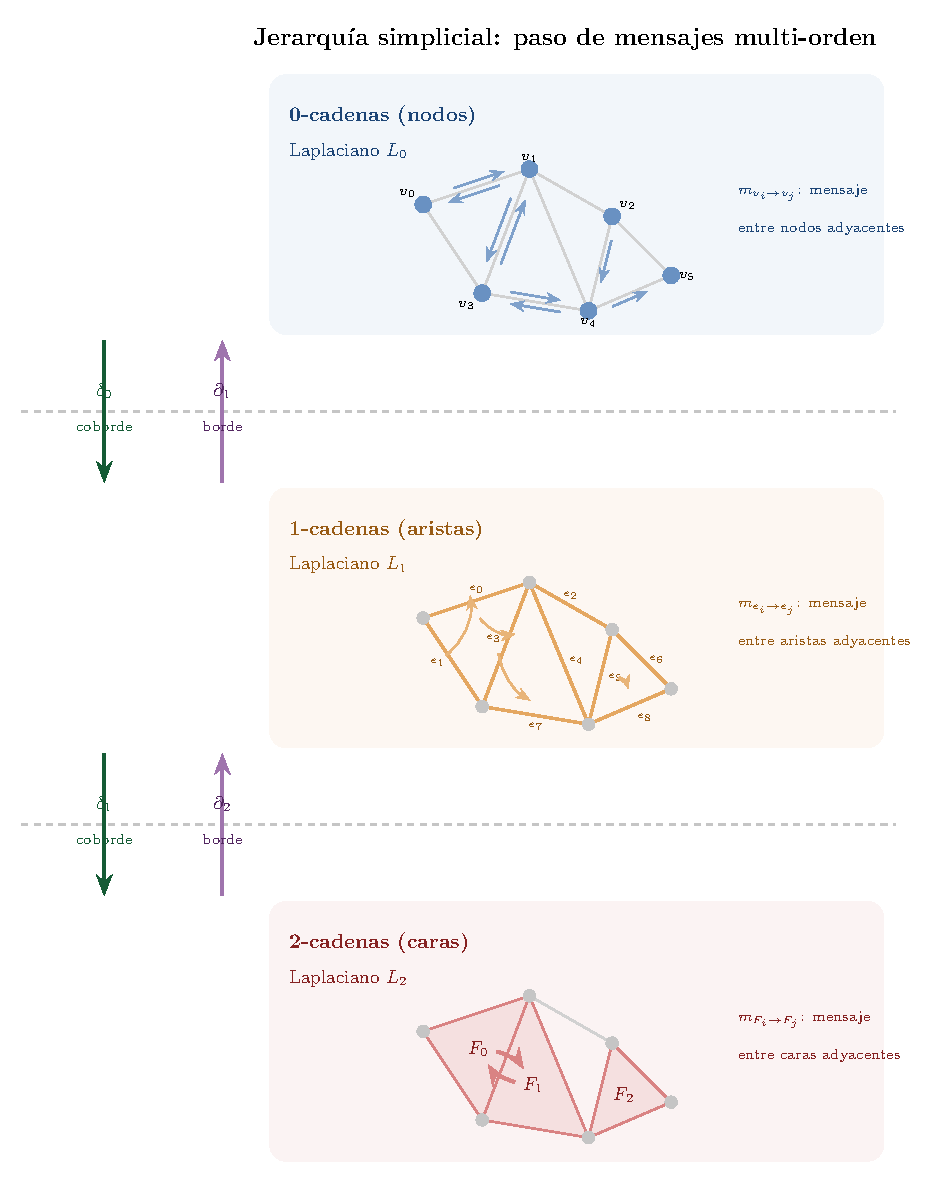
\includegraphics[width=0.85\textwidth]{images/simplicial_hierarchy}
	\caption[Jerarquía simplicial: paso de mensajes multi-orden]{Jerarquía de paso de mensajes en un complejo simplicial: mensajes entre nodos (0-cadenas), aristas (1-cadenas) y caras (2-cadenas), conectados por operadores frontera $\partial_k$ y cofrontera $\delta_k$. El Laplaciano de Hodge $L_k$ captura la interacción entre niveles adyacentes.}
	\label{fig:simplicial_hierarchy}
\end{figure}

\subsubsection{Laplacianos de Hodge}

Los Laplacianos de Hodge son operadores fundamentales que extienden el Laplaciano de grafos a complejos de dimensión superior (para la definición general y sus propiedades, véase la \autoref{def:hodge_laplacian_gdl} y la \autoref{prop:propiedades_hodge_gdl} del \autoref{ch:gdl}).

\begin{definition}[Operador Cofrontera]\label{def:cofrontera}
El \textbf{operador cofrontera} $\delta_k: C_k \to C_{k+1}$ es el adjunto formal de $\partial_{k+1}$:
\[\delta_k = \partial_{k+1}^T\]
respecto al producto interior estándar en espacios de cadenas.
\end{definition}

\begin{definition}[Laplacianos de Hodge]\label{def:hodge_laplacians_cnn}
El \textbf{Laplaciano de Hodge} de orden $k$ es:
\[L_k = \partial_{k+1} \partial_{k+1}^T + \partial_k^T \partial_k = \delta_{k-1} \delta_{k-1}^T + \delta_k^T \delta_k\]

Descomposición en dos términos:
\begin{itemize}
    \item $L_k^{\text{down}} = \partial_k^T \partial_k$: Laplaciano inferior (flujo desde $(k-1)$-cadenas)
    \item $L_k^{\text{up}} = \partial_{k+1} \partial_{k+1}^T$: Laplaciano superior (flujo hacia $(k+1)$-cadenas)
\end{itemize}
\end{definition}

\begin{theorem}[Propiedades del Laplaciano de Hodge]\label{thm:prop_hodge_laplacian}
El Laplaciano $L_k$ satisface:
\begin{enumerate}
    \item \textbf{Simetría}: $L_k$ es simétrico y semidefinido positivo
    \item \textbf{Kernel y homología}: $\ker(L_k) \cong H_k(\mathcal{K})$ (grupo de homología de dimensión $k$)
    \item \textbf{Descomposición de Hodge}:
    \[C_k = \text{Im}(\partial_{k+1}) \oplus \ker(L_k) \oplus \text{Im}(\partial_k^T)\]
\end{enumerate}
\end{theorem}

\begin{proof}
(1) \textit{Simetría}: $L_k = \partial_k^T \partial_k + \partial_{k+1} \partial_{k+1}^T$ es suma de matrices de la forma $A^T A$, que son simétricas y semidefinidas positivas. Para ver que $L_k$ es semidefinida positiva: $\langle L_k \mathbf{x}, \mathbf{x} \rangle = \|\partial_k \mathbf{x}\|^2 + \|\partial_{k+1}^T \mathbf{x}\|^2 \geq 0$.

(2) \textit{Kernel y homología}: $L_k \mathbf{x} = 0$ si y solo si $\|\partial_k \mathbf{x}\|^2 + \|\partial_{k+1}^T \mathbf{x}\|^2 = 0$, es decir, $\partial_k \mathbf{x} = 0$ y $\partial_{k+1}^T \mathbf{x} = 0$. La primera condición dice que $\mathbf{x}$ es un $k$-ciclo ($\mathbf{x} \in \ker \partial_k$) y la segunda que $\mathbf{x}$ es ortogonal a la imagen de $\partial_{k+1}$ ($\mathbf{x} \perp \operatorname{Im} \partial_{k+1}$). Luego $\ker L_k = \ker \partial_k \cap (\operatorname{Im} \partial_{k+1})^\perp$, que es el representante armónico de la clase de homología $H_k = \ker \partial_k / \operatorname{Im} \partial_{k+1}$.

(3) \textit{Descomposición de Hodge}: Los tres subespacios son mutuamente ortogonales: $\operatorname{Im}(\partial_{k+1}) \perp \operatorname{Im}(\partial_k^T)$ porque $\partial_k \partial_{k+1} = 0$ (propiedad fundamental de los operadores frontera). El kernel $\ker L_k$ es el complemento ortogonal de $\operatorname{Im}(\partial_{k+1}) \oplus \operatorname{Im}(\partial_k^T)$ en $C_k$.
\end{proof}

\begin{example}[Laplaciano de Hodge para Malla Triangular]\label{ex:hodge_triangle_mesh}
Consideremos una malla triangular simple con 4 vértices formando dos triángulos adyacentes.

\textbf{Estructura:}
\begin{itemize}
    \item Vértices: $v_0, v_1, v_2, v_3$
    \item Aristas: $e_1 = [v_0,v_1], e_2 = [v_1,v_2], e_3 = [v_0,v_2], e_4 = [v_1,v_3], e_5 = [v_2,v_3]$
    \item Triángulos: $\tau_1 = [v_0,v_1,v_2], \tau_2 = [v_1,v_2,v_3]$
\end{itemize}

\textbf{Matriz de frontera $\partial_1$ (aristas $\to$ vértices):}
\[\partial_1 = \begin{pmatrix}
-1 & 0 & -1 & 0 & 0 \\
1 & -1 & 0 & -1 & 0 \\
0 & 1 & 1 & 0 & -1 \\
0 & 0 & 0 & 1 & 1
\end{pmatrix}\]

\textbf{Matriz de frontera $\partial_2$ (triángulos $\to$ aristas):}

Para $\tau_1 = [v_0,v_1,v_2]$: $\partial_2(\tau_1) = [v_1,v_2] - [v_0,v_2] + [v_0,v_1] = e_2 - e_3 + e_1$.
Para $\tau_2 = [v_1,v_2,v_3]$: $\partial_2(\tau_2) = [v_2,v_3] - [v_1,v_3] + [v_1,v_2] = e_5 - e_4 + e_2$.
\[\partial_2 = \begin{pmatrix}
1 & 0 \\
1 & 1 \\
-1 & 0 \\
0 & -1 \\
0 & 1
\end{pmatrix}\]

Se verifica que $\partial_1 \partial_2 = 0$, consistente con el \autoref{thm:partial_squared}.

\textbf{Laplaciano de aristas (1-Laplaciano):}
\[L_1 = \partial_1^T \partial_1 + \partial_2 \partial_2^T\]

Este operador captura tanto la conectividad entre aristas vía vértices comunes como vía triángulos comunes.
\end{example}

\subsubsection{Topological Deep Learning: Arquitecturas}

El trabajo comprehensivo de \citet{hajij2023topological} establece las bases teóricas y prácticas del aprendizaje profundo topológico.

\begin{definition}[Complejo Combinatorial]\label{def:complejo_combinatorial}
Un \textbf{complejo combinatorial} $\mathcal{K}$ es una colección de conjuntos finitos (células) equipada con una relación de inclusión parcial, que generaliza tanto complejos simpliciales como celulares sin imponer condiciones restrictivas de frontera.
\end{definition}

Esta definición generaliza las estructuras de datos relacionales tradicionales:
\begin{itemize}
    \item \textbf{Grafos:} Caso especial con células de dimensión 0 y 1
    \item \textbf{Hipergrafos:} Subconjunto con hiperejes de dimensión variable
    \item \textbf{Complejos simpliciales:} Caso restringido con relaciones de frontera específicas
    \item \textbf{Complejos celulares:} Generalizaciones con células de formas arbitrarias
\end{itemize}

\textbf{Combinatorial Complex Neural Networks (CCNNs):}

Las CCNNs operan mediante propagación de mensajes multi-nivel entre células de diferentes dimensiones:
\[h_\sigma^{(l+1)} = \text{UPDATE}\left(h_\sigma^{(l)}, \text{AGGREGATE}\left(\{h_\tau^{(l)} : \tau \in \mathcal{N}(\sigma)\}\right)\right)\]
donde $\mathcal{N}(\sigma)$ representa el vecindario de la célula $\sigma$, que puede incluir células de diversas dimensiones.

\begin{definition}[Vecindarios en Complejos]\label{def:vecindarios_complejos}
Para una $k$-célula $\sigma$ en un complejo, definimos:
\begin{itemize}
    \item \textbf{Vecindario inferior}: $\mathcal{N}_{\text{low}}(\sigma) = \{\tau : \tau \subseteq \sigma, \dim(\tau) = k-1\}$
    \item \textbf{Vecindario superior}: $\mathcal{N}_{\text{up}}(\sigma) = \{\tau : \sigma \subseteq \tau, \dim(\tau) = k+1\}$
    \item \textbf{Vecindario co-dimensional}: $\mathcal{N}_{\text{co}}(\sigma) = \{\tau : \dim(\tau) = k, \tau \cap \sigma \neq \emptyset\}$
\end{itemize}
\end{definition}

\textbf{Operadores de Frontera y Co-frontera:}

La estructura topológica se captura mediante operadores lineales derivados de los operadores de frontera algebraicos:
\begin{itemize}
    \item \textbf{Operador de frontera} $\partial_k: C_k \to C_{k-1}$ (véase \autoref{def:cadenas_frontera})
    \item \textbf{Operador de co-frontera} $\delta_k = \partial_{k+1}^T: C_k \to C_{k+1}$
\end{itemize}

Estos operadores definen las matrices de adyacencia generalizadas que rigen el paso de mensajes.

\textbf{Propiedades de Equivarianza:}

Las CCNNs mantienen equivarianza bajo:
\begin{enumerate}
    \item \textbf{Permutaciones}: Reordenamiento de células dentro de la misma dimensión
    \item \textbf{Orientaciones}: Cambios en la orientación de células orientadas
    \item \textbf{Transformaciones topológicas}: Homeomorfismos que preservan la estructura
\end{enumerate}

\subsubsection{Simplicial Attention Networks}

El trabajo de \citet{giusti2022simplicial} introduce mecanismos de atención específicamente diseñados para complejos simpliciales, combinando la expresividad topológica con la flexibilidad de la atención.

\textbf{Complejos Simpliciales:}

\begin{definition}[Complejo Simplicial]
Un \textbf{complejo simplicial} $\mathcal{K}$ es una colección de simplicios que satisface:
\begin{enumerate}
    \item Si $\sigma \in \mathcal{K}$ y $\tau \subseteq \sigma$, entonces $\tau \in \mathcal{K}$ (clausura hacia abajo)
    \item La intersección de dos simplicios es vacía o un simplicio común
\end{enumerate}
\end{definition}

\textbf{Mecanismo de Atención Simplicial:}

Para un $k$-simplicio $\sigma$ y su vecindario $N(\sigma)$:
\[\alpha_{\sigma,\tau} = \text{softmax}\left(\text{LeakyReLU}\left(a^T[W_\sigma h_\sigma \| W_\tau h_\tau \| o_{\sigma,\tau}]\right)\right)\]
donde:
\begin{itemize}
    \item $h_\sigma, h_\tau$: Representaciones de simplicios
    \item $W_\sigma, W_\tau$: Matrices de transformación aprendibles
    \item $a$: Vector de atención aprendible
    \item $o_{\sigma,\tau}$: Información de orientación relativa
\end{itemize}

\textbf{Atención con Orientación (Signed Attention):}

Una característica distintiva es la incorporación de información de orientación:
\[\alpha'_{\sigma,\tau} = s_{\sigma,\tau} \cdot \alpha_{\sigma,\tau}\]
donde $s_{\sigma,\tau} \in \{-1, +1\}$ refleja la orientación relativa entre simplicios.

Esta atención orientada preserva las propiedades cohomológicas del complejo y mantiene equivarianza bajo cambios de orientación:
\[\text{SAT}(\mathcal{O}(X)) = \mathcal{O}(\text{SAT}(X))\]
para un cambio de orientación $\mathcal{O}$.

\textbf{Procesamiento Multi-dimensional:}

Las SATs procesan información en múltiples dimensiones simultáneamente:
\begin{itemize}
    \item \textbf{Capas paralelas:} Procesamiento independiente por dimensión
    \item \textbf{Comunicación inter-dimensional:} Flujo de información via operadores de frontera
    \item \textbf{Agregación jerárquica:} Pooling topológicamente consciente
\end{itemize}

\subsubsection{Complejos CW y Aplicaciones}

Los complejos CW (Closure-finite, Weak topology) proporcionan un marco aún más general que los complejos simpliciales, permitiendo células de formas arbitrarias adheridas de manera topológicamente coherente.

\textbf{Definición y Estructura:}

\begin{definition}[Complejo CW]
Un \textbf{complejo CW} es un espacio topológico $X$ junto con una descomposición en células $e^n_\alpha$ de dimensión $n$, donde cada célula se adhiere al esqueleto de dimensión inferior mediante una aplicación característica continua.
\end{definition}

\textbf{Ventajas para Deep Learning:}
\begin{enumerate}
    \item \textbf{Flexibilidad geométrica:} Células de formas arbitrarias
    \item \textbf{Eficiencia representacional:} Menos células que representaciones simpliciales equivalentes
    \item \textbf{Compatibilidad computacional:} Estructura regular compatible con paralelización
\end{enumerate}

\textbf{Aplicaciones Emergentes:}
\begin{itemize}
    \item \textbf{Análisis de imágenes:} Segmentación basada en estructura topológica
    \item \textbf{Modelado molecular:} Representación de complejos proteicos
    \item \textbf{Neurociencia:} Análisis de conectomas cerebrales
    \item \textbf{Análisis de redes sociales:} Modelado de comunidades jerárquicas
\end{itemize}

\subsection{Conexiones entre Álgebra y Topología}

La verdadera potencia de las extensiones algebraicas avanzadas emerge de las conexiones profundas entre estructuras algebraicas y topológicas. Estas conexiones no son meramente teóricas, sino que proporcionan principios unificadores para el diseño de arquitecturas de \gls{GDL}.

\subsubsection{Homología y Cohomología}

La homología y cohomología proporcionan invariantes algebraicos de espacios topológicos que son fundamentales para el \gls{GDL}.

Recordamos que el $k$-ésimo grupo de homología $H_k(\mathcal{K}) = Z_k / B_k$ mide los ``agujeros $k$-dimensionales'' del complejo (\autoref{def:homologia_betti} del \autoref{ch:gdl}).\label{def:grupos_homologia_cnn}

\textbf{Interpretación Geométrica.}\label{rem:interp_homologia} $H_k(\mathcal{K})$ mide los "agujeros $k$-dimensionales" del espacio:
\begin{itemize}
    \item $H_0$: Componentes conexas
    \item $H_1$: Ciclos no triviales (túneles, loops)
    \item $H_2$: Cavidades (voids)
    \item $H_k$ ($k > 2$): Agujeros de dimensión superior
\end{itemize}

\begin{definition}[Números de Betti]\label{def:numeros_betti_cnn}
El \textbf{$k$-ésimo número de Betti} es:
\[\beta_k = \dim(H_k(\mathcal{K})) = \text{rango}(Z_k) - \text{rango}(B_k)\]
\end{definition}

\begin{example}[Homología de Esfera y Toro]\label{ex:homologia_esfera_toro}
\textbf{Esfera $S^2$:}
\begin{align}
H_0(S^2) &\cong \mathbb{R} \quad (\beta_0 = 1, \text{ conexa}) \\
H_1(S^2) &= 0 \quad (\beta_1 = 0, \text{ sin loops}) \\
H_2(S^2) &\cong \mathbb{R} \quad (\beta_2 = 1, \text{ cavidad})
\end{align}

\textbf{Toro $T^2 = S^1 \times S^1$:}
\begin{align}
H_0(T^2) &\cong \mathbb{R} \quad (\beta_0 = 1) \\
H_1(T^2) &\cong \mathbb{R}^2 \quad (\beta_1 = 2, \text{ dos loops independientes}) \\
H_2(T^2) &\cong \mathbb{R} \quad (\beta_2 = 1)
\end{align}

La característica de Euler:
\[\chi(S^2) = \beta_0 - \beta_1 + \beta_2 = 1 - 0 + 1 = 2\]
\[\chi(T^2) = \beta_0 - \beta_1 + \beta_2 = 1 - 2 + 1 = 0\]
\end{example}

\begin{definition}[Cohomología de De Rham]\label{def:cohomologia_derham}
En variedades diferenciables, la \textbf{cohomología de De Rham} $H^k_{\text{dR}}(\mathcal{M})$ se define como:
\[H^k_{\text{dR}}(\mathcal{M}) = \frac{\ker(d: \Omega^k \to \Omega^{k+1})}{\text{Im}(d: \Omega^{k-1} \to \Omega^k)}\]
donde $\Omega^k$ es el espacio de $k$-formas diferenciales y $d$ es la derivada exterior.
\end{definition}

\begin{theorem}[Teorema de De Rham]\label{thm:derham}
Para una variedad diferenciable $\mathcal{M}$:
\[H^k_{\text{dR}}(\mathcal{M}) \cong H^k(\mathcal{M}; \mathbb{R})\]
La cohomología de De Rham es isomorfa a la cohomología singular con coeficientes reales.

Véase la Sección~\ref{sec:de_rham} del \autoref{ch:teoremas_complementarios} para la demostración.
\end{theorem}

\subsubsection{Álgebra Exterior y Conexión con Clifford}

El álgebra exterior proporciona el puente entre álgebras de Clifford y topología algebraica.

\begin{definition}[Álgebra Exterior]\label{def:algebra_exterior}
Sea $V$ un espacio vectorial. El \textbf{álgebra exterior} $\bigwedge V$ es el álgebra graduada:
\[\bigwedge V = \bigoplus_{k=0}^n \bigwedge^k V\]
donde $\bigwedge^k V$ es el espacio de $k$-vectores con producto exterior $\wedge$ antisimétrico:
\[v \wedge w = -w \wedge v, \quad v \wedge v = 0\]
\end{definition}

\textbf{Relación Clifford-Exterior.}\label{rem:clifford_exterior} El álgebra de Clifford $\text{Cl}(V, Q)$ y el álgebra exterior $\bigwedge V$ están relacionadas:
\begin{itemize}
    \item Como espacios vectoriales: $\text{Cl}(V,Q) \cong \bigwedge V$ (ambos tienen dimensión $2^n$)
    \item El producto geométrico extiende el producto exterior: $uv = u \cdot v + u \wedge v$
    \item $\bigwedge V = \text{Cl}(V, 0)$ (álgebra de Clifford con forma cuadrática nula)
\end{itemize}

\begin{example}[Base del Álgebra Exterior $\bigwedge \mathbb{R}^3$]\label{ex:base_exterior_3d}
Para $V = \mathbb{R}^3$ con base $\{e_1, e_2, e_3\}$:
\begin{align}
\bigwedge^0 \mathbb{R}^3 &: \{1\} \quad \text{(escalares)} \\
\bigwedge^1 \mathbb{R}^3 &: \{e_1, e_2, e_3\} \quad \text{(vectores)} \\
\bigwedge^2 \mathbb{R}^3 &: \{e_1 \wedge e_2, e_1 \wedge e_3, e_2 \wedge e_3\} \quad \text{(bivectores)} \\
\bigwedge^3 \mathbb{R}^3 &: \{e_1 \wedge e_2 \wedge e_3\} \quad \text{(pseudoescalar)}
\end{align}
Total: $1 + 3 + 3 + 1 = 8$ dimensiones.
\end{example}

\subsubsection{Homología Persistente}

La homología persistente proporciona una herramienta multiescala para análisis topológico de datos.

\begin{definition}[Filtración]\label{def:filtracion_cnn}
Una \textbf{filtración} de un complejo simplicial es una secuencia anidada:
\[\emptyset = \mathcal{K}_0 \subseteq \mathcal{K}_1 \subseteq \mathcal{K}_2 \subseteq \cdots \subseteq \mathcal{K}_m = \mathcal{K}\]
donde cada $\mathcal{K}_i$ es un subcomplejo de $\mathcal{K}$.
\end{definition}

\begin{definition}[Diagrama de Persistencia]\label{def:diagrama_persistencia_cnn}
El \textbf{diagrama de persistencia} registra los pares $(b, d)$ donde:
\begin{itemize}
    \item $b$ (birth): Escala en que aparece un ciclo homológico
    \item $d$ (death): Escala en que el ciclo desaparece
    \item Persistencia: $\text{pers}(b,d) = d - b$
\end{itemize}
\end{definition}

\textbf{Aplicaciones en GDL.}\label{rem:persistencia_gdl} La homología persistente se usa en:
\begin{itemize}
    \item \textbf{Featurización}: Diagramas de persistencia como características para CNNs
    \item \textbf{Pooling topológico}: Preservar estructuras persistentes
    \item \textbf{Regularización}: Penalizar topologías indeseadas
\end{itemize}

\subsubsection{Teoría de Sheaves}

La teoría de sheaves proporciona un framework para datos distribuidos sobre espacios topológicos.

\begin{definition}[Sheaf Celular]\label{def:sheaf_celular}
Un \textbf{sheaf celular} $\mathcal{F}$ sobre un complejo celular $X$ asigna:
\begin{itemize}
    \item A cada célula $\sigma \in X$ un espacio vectorial $\mathcal{F}(\sigma)$ (stalk)
    \item A cada par $\tau \subseteq \sigma$ un mapa de restricción $\mathcal{F}_{\sigma \to \tau}: \mathcal{F}(\sigma) \to \mathcal{F}(\tau)$
\end{itemize}
satisfaciendo propiedades de composición.
\end{definition}

\textbf{Sheaf Neural Networks.}\label{rem:sheaf_nns} Las Sheaf Neural Networks de \citet{hansen2021sheaf} y \citet{bodnar2023cellular} usan sheaves para modelar:
\begin{itemize}
    \item \textbf{Heterogeneidad}: Diferentes espacios de características en cada célula
    \item \textbf{Alineamiento}: Mapas de restricción como transformaciones de alineamiento
    \item \textbf{Coherencia}: Minimizar desalineamiento en el paso de mensajes
\end{itemize}

\begin{example}[Sheaf Laplacian]\label{ex:sheaf_laplacian}
Para un sheaf $\mathcal{F}$ sobre grafo $G$, el \textbf{Laplaciano de sheaf} es:
\[L_{\mathcal{F}} = \delta^T \delta\]
donde $\delta$ incorpora los mapas de restricción:
\[(\delta f)_e = \mathcal{F}_{t(e) \to e}(f_{t(e)}) - \mathcal{F}_{s(e) \to e}(f_{s(e)})\]
para arista $e$ con source $s(e)$ y target $t(e)$.

Generaliza el Laplaciano de grafo estándar permitiendo espacios de características heterogéneos.
\end{example}

\subsubsection{Invariantes Topológicos Aprendibles}

Las arquitecturas avanzadas pueden aprender a computar invariantes topológicos como:
\begin{itemize}
    \item \textbf{Números de Betti:} Dimensiones de grupos de homología (\autoref{def:numeros_betti_cnn})
    \item \textbf{Característica de Euler:} Suma alternada de números de Betti: $\chi = \sum_k (-1)^k \beta_k$
    \item \textbf{Clases características:} Invariantes diferenciables de fibrados
    \item \textbf{Diagramas de persistencia:} Representaciones multiescala de topología
\end{itemize}

Estos invariantes proporcionan representaciones robustas y geométricamente significativas para el aprendizaje.

\subsubsection{Perspectivas Categóricas}

La teoría de categorías proporciona un lenguaje unificador que conecta álgebras de Clifford, complejos topológicos y arquitecturas de redes neuronales.

\textbf{Funtores y Equivalencias.}\label{rem:funtores_equivalencias} Los funtores entre categorías geométricas formalizan las transformaciones de representación:
\begin{itemize}
    \item \textbf{Funtor de chains}: $C_*: \textbf{Top} \to \textbf{Chain}$ (espacios a complejos de cadenas)
    \item \textbf{Funtor de homología}: $H_*: \textbf{Chain} \to \textbf{GrVect}$ (cadenas a espacios graduados)
    \item \textbf{Funtor de Clifford}: Asocia a cada variedad Riemanniana su Clifford bundle
\end{itemize}

Las extensiones algebraicas avanzadas (Clifford, topológicas, categóricas) enfrentan desafíos computacionales de escalabilidad y estabilidad numérica en álgebras de alta dimensión, y requieren mayor desarrollo teórico en capacidades expresivas y garantías de convergencia.

\section{Métodos Especiales y Conexiones}\label{sec:special_methods}

Esta sección final del capítulo explora métodos especializados que complementan las técnicas convolucionales geométricas presentadas anteriormente, estableciendo conexiones con otros paradigmas de aprendizaje y analizando perspectivas futuras del campo. Los temas tratados incluyen codificación posicional avanzada, ruptura controlada de simetrías, aplicaciones en computación cuántica, y consideraciones de escalabilidad que determinan la viabilidad práctica de estos métodos.

\subsection{Codificación Posicional y Features de Fourier}

\subsubsection{Fundamentos de la Codificación Posicional}

La codificación posicional representa un desafío fundamental en el aprendizaje geométrico: cómo representar información espacial de manera que preserve tanto la estructura local como las relaciones globales. Las CNNs tradicionales incorporan información posicional implícitamente a través de la estructura de vecindad de las convoluciones, pero en contextos geométricos más generales esta aproximación resulta insuficiente.

El trabajo seminal de \citet{tancik2020fourier} demostró que las redes neuronales estándar tienen dificultades para aprender funciones que varían rápidamente en dominios de baja dimensión. Este problema surge porque las redes con activaciones \gls{ReLU} están naturalmente sesgadas hacia funciones suaves, una limitación que se manifiesta especialmente en tareas que requieren capturar detalles de alta frecuencia.

\begin{theorem}[Sesgo de Frecuencia en Redes Neuronales]
Sea $f: \mathbb{R}^d \to \mathbb{R}$ una función objetivo con componentes espectrales significativas en altas frecuencias. Una red neuronal $\mathcal{F}_\theta$ entrenada mediante descenso de gradiente en el espacio de parámetros $\theta$ exhibe un sesgo hacia la aproximación de componentes de baja frecuencia de $f$ durante las primeras iteraciones del entrenamiento.
\end{theorem}

Este sesgo se origina en la inicialización de pesos y la naturaleza del gradiente descendente, que tiende a explorar primero las componentes del espacio de funciones de menor complejidad. Matemáticamente, consideremos el desarrollo de Fourier de la función objetivo:
\begin{equation}
f(\mathbf{x}) = \sum_{\omega \in \mathbb{Z}^d} \hat{f}(\omega) e^{2\pi i \omega \cdot \mathbf{x}}
\end{equation}

Durante las primeras épocas de entrenamiento, la red aproxima preferentemente los coeficientes $\hat{f}(\omega)$ con $\|\omega\|$ pequeño, postergando la captura de componentes de alta frecuencia.

\subsubsection{Random Fourier Features: Teoría Fundacional}

El trabajo pionero de Rahimi \& Recht (NIPS 2007) estableció los fundamentos teóricos de las random Fourier features para aproximar kernels en máquinas de kernel a gran escala. Este enfoque se ha convertido en una herramienta fundamental para la codificación posicional en aprendizaje geométrico.

\begin{theorem}[Teorema de Bochner]\label{thm:bochner}
Un kernel continuo $k: \mathbb{R}^d \times \mathbb{R}^d \to \mathbb{R}$ es invariante por traslación (i.e., $k(\mathbf{x}, \mathbf{y}) = k(\mathbf{x} - \mathbf{y})$) y positivo definido si y solo si existe una medida de probabilidad finita no negativa $\mu$ tal que:
\begin{equation}
k(\mathbf{x} - \mathbf{y}) = \int_{\mathbb{R}^d} e^{2\pi i \omega^T (\mathbf{x} - \mathbf{y})} d\mu(\omega)
\end{equation}
\end{theorem}

\begin{proof}
La dirección directa sigue de propiedades básicas de la transformada de Fourier. Para la dirección inversa, la función $\phi(\mathbf{x}) = k(\mathbf{x}, \mathbf{0}) = k(\mathbf{x})$ es continua y positiva definida. Por el teorema de Bochner clásico, $\phi$ admite representación como transformada de Fourier de una medida finita no negativa.
\end{proof}

El teorema de Bochner proporciona la justificación matemática para aproximar kernels mediante muestreo Monte Carlo de su transformada de Fourier. Si $p(\omega)$ es la densidad asociada a $\mu$, podemos aproximar:
\begin{equation}
k(\mathbf{x}, \mathbf{y}) \approx \frac{1}{m} \sum_{j=1}^m \cos(2\pi \omega_j^T \mathbf{x}) \cos(2\pi \omega_j^T \mathbf{y}) + \sin(2\pi \omega_j^T \mathbf{x}) \sin(2\pi \omega_j^T \mathbf{y})
\end{equation}
donde $\omega_j \sim p(\omega)$ son frecuencias muestreadas independientemente.

\paragraph{Construcción del Mapeo de Features}

Definimos el mapeo de random Fourier features como:
\begin{equation}
z(\mathbf{x}) = \sqrt{\frac{2}{m}} \begin{bmatrix} \cos(2\pi \omega_1^T \mathbf{x}) \\ \vdots \\ \cos(2\pi \omega_m^T \mathbf{x}) \\ \sin(2\pi \omega_1^T \mathbf{x}) \\ \vdots \\ \sin(2\pi \omega_m^T \mathbf{x}) \end{bmatrix} \in \mathbb{R}^{2m}
\end{equation}

Este mapeo satisface la propiedad fundamental:
\begin{equation}
\mathbb{E}_{\omega \sim p}[z(\mathbf{x})^T z(\mathbf{y})] = k(\mathbf{x}, \mathbf{y})
\end{equation}

\begin{theorem}[Convergencia de Random Fourier Features]
Sea $k$ un kernel Gaussiano $k(\mathbf{x}, \mathbf{y}) = \exp(-\|\mathbf{x} - \mathbf{y}\|^2 / 2\sigma^2)$ y $\hat{k}_m$ su aproximación mediante $m$ random Fourier features. Entonces, para cualquier $\epsilon, \delta > 0$, si:
\begin{equation}
m \geq \frac{4}{\epsilon^2} \log\left(\frac{2n}{\delta}\right)
\end{equation}
se tiene que con probabilidad al menos $1 - \delta$:
\begin{equation}
\sup_{\mathbf{x}, \mathbf{y} \in \mathcal{X}} |k(\mathbf{x}, \mathbf{y}) - \hat{k}_m(\mathbf{x}, \mathbf{y})| \leq \epsilon
\end{equation}
donde $\mathcal{X} \subset \mathbb{R}^d$ es un conjunto compacto de $n$ puntos.

Véase la Sección~\ref{sec:convergencia_rff} del \autoref{ch:teoremas_complementarios} para la demostración completa.
\end{theorem}

Este resultado garantiza convergencia uniforme de la aproximación con tasa $O(1/\sqrt{m})$, proporcionando garantías teóricas rigurosas para el uso de random Fourier features en codificación posicional.

\subsubsection{Features de Fourier como Codificación Universal}

La solución propuesta por Tancik et al. consiste en transformar las coordenadas de entrada mediante features de Fourier antes de procesarlas con la red neuronal. Para una entrada $\mathbf{x} \in \mathbb{R}^d$, la transformación de features de Fourier se define como:

\begin{equation}
\gamma(\mathbf{x}) = \left[\sin(2\pi \mathbf{B}\mathbf{x}), \cos(2\pi \mathbf{B}\mathbf{x})\right]^T
\end{equation}

donde $\mathbf{B} \in \mathbb{R}^{m \times d}$ es una matriz de frecuencias muestreada de una distribución gaussiana $\mathcal{N}(0, \sigma^2)$. El parámetro $\sigma$ controla el espectro de frecuencias: valores pequeños favorecen funciones suaves mientras que valores grandes permiten capturar variaciones de alta frecuencia.

\begin{definition}[Mapeo de Features de Fourier]
Un mapeo de features de Fourier $\gamma: \mathbb{R}^d \to \mathbb{R}^{2m}$ es una transformación que proyecta coordenadas espaciales a un espacio de características donde las funciones periódicas de diferentes frecuencias pueden ser representadas linealmente.
\end{definition}

\paragraph{Análisis Espectral y Elección de $\sigma$}

La elección del parámetro de escala $\sigma$ en la distribución de frecuencias es crucial. Para kernels Gaussianos RBF $k(\mathbf{x}, \mathbf{y}) = \exp(-\|\mathbf{x} - \mathbf{y}\|^2 / 2\gamma^2)$, la distribución de frecuencias óptima es $p(\omega) \propto \exp(-\|\omega\|^2 \gamma^2 / 2)$, es decir, $\omega \sim \mathcal{N}(0, \gamma^{-2} \mathbf{I})$.

En la práctica, $\sigma$ se selecciona mediante validación cruzada o siguiendo heurísticas basadas en la escala característica de los datos:
\begin{equation}
\sigma_{\text{óptimo}} \approx \frac{1}{\text{mediana}(\{\|\mathbf{x}_i - \mathbf{x}_j\| : i, j \in [n]\})}
\end{equation}

\paragraph{Ejemplo Trabajado: Codificación en $\mathbb{R}^2$}

Consideremos coordenadas espaciales $\mathbf{x} = (x, y) \in [0, 1]^2$ y $m = 3$ componentes de frecuencia. Muestreamos:
\begin{align}
\omega_1 &= (2.1, -1.3)^T, \quad \omega_2 = (-0.8, 3.4)^T, \quad \omega_3 = (1.7, 2.2)^T
\end{align}

La codificación de Fourier para un punto $\mathbf{x}_0 = (0.5, 0.5)$ es:
\begin{align}
\gamma(\mathbf{x}_0) = [&\sin(2\pi \cdot 0.4), \sin(2\pi \cdot 1.3), \sin(2\pi \cdot 1.95), \\
&\cos(2\pi \cdot 0.4), \cos(2\pi \cdot 1.3), \cos(2\pi \cdot 1.95)]^T
\end{align}

Esta codificación captura información sobre la posición en múltiples escalas de frecuencia simultáneamente.

\subsubsection{Conexión con Análisis Armónico en Variedades}

Esta técnica tiene implicaciones profundas para las CNNs geométricas. En variedades Riemannianas, las coordenadas geodésicas pueden ser enriquecidas con features de Fourier para capturar variaciones locales de alta frecuencia mientras se preserva la estructura global de la variedad.

El análisis armónico en variedades proporciona el marco teórico para extender random Fourier features a dominios no euclidianos. Sea $(\mathcal{M}, g)$ una variedad Riemanniana compacta con operador de Laplace-Beltrami $\Delta_{\mathcal{M}}$. Los eigenfunciones $\{\phi_k\}$ del laplaciano forman una base ortonormal completa de $L^2(\mathcal{M})$:
\begin{equation}
\Delta_{\mathcal{M}} \phi_k = -\lambda_k \phi_k, \quad \int_{\mathcal{M}} \phi_i \phi_j \, dV_g = \delta_{ij}
\end{equation}

\begin{proposition}[Features de Fourier en Variedades]
Para una variedad Riemanniana compacta $\mathcal{M}$, un mapeo de features basado en eigenfunciones del laplaciano:
\begin{equation}
\gamma_{\mathcal{M}}(p) = \sqrt{\frac{2}{m}} \begin{bmatrix} \phi_1(p) \\ \vdots \\ \phi_m(p) \end{bmatrix}
\end{equation}
aproxima kernels de difusión $k_t(p, q) = \sum_{k=1}^\infty e^{-t\lambda_k} \phi_k(p)\phi_k(q)$ con error $O(e^{-t\lambda_{m+1}})$.
\end{proposition}

\begin{proof}
El kernel de difusión se expande como $k_t(p,q) = \sum_{k=1}^{\infty} e^{-t\lambda_k} \phi_k(p) \phi_k(q)$, donde $\{\lambda_k, \phi_k\}$ son los pares propios del Laplaciano de Beltrami en $\mathcal{M}$ con $0 \leq \lambda_1 \leq \lambda_2 \leq \cdots$. La aproximación con $m$ eigenfunciones trunca la serie: $\hat{k}_t(p,q) = \sum_{k=1}^{m} e^{-t\lambda_k} \phi_k(p) \phi_k(q)$. El error de truncamiento es:
\[
|k_t(p,q) - \hat{k}_t(p,q)| = \left|\sum_{k=m+1}^{\infty} e^{-t\lambda_k} \phi_k(p) \phi_k(q)\right| \leq e^{-t\lambda_{m+1}} \sum_{k=m+1}^{\infty} |\phi_k(p) \phi_k(q)|
\]
donde usamos $e^{-t\lambda_k} \leq e^{-t\lambda_{m+1}}$ para $k > m$. La convergencia de la serie residual está garantizada por la ley de Weyl ($\lambda_k \sim k^{2/\dim \mathcal{M}}$) y la acotación uniforme de las eigenfunciones en variedades compactas.
\end{proof}

Este resultado establece que las eigenfunciones del laplaciano en variedades generalizan las funciones sinusoidales del caso euclidiano, proporcionando una teoría unificada de codificación posicional.

\subsubsection{Integración con CNNs Equivariantes}

La combinación de features de Fourier con CNNs equivariantes requiere cuidado especial para preservar las propiedades de simetría. Sea $g \in G$ una transformación del grupo de simetrías y $\mathbf{x}$ una coordenada espacial. Para que la codificación sea equivariante, debe satisfacerse:

\begin{equation}
\gamma(g \cdot \mathbf{x}) = \rho(g) \gamma(\mathbf{x})
\end{equation}

donde $\rho: G \to \text{GL}(\mathbb{R}^{2m})$ es una representación del grupo en el espacio de features.

Para grupos de rotación $\text{SO}(2)$, esto se logra utilizando armónicos circulares como base para las features de Fourier. Específicamente, para $G = \text{SO}(2)$, las frecuencias $\omega$ deben seleccionarse de modo que $\omega \cdot (R\mathbf{x}) = (R^T\omega) \cdot \mathbf{x}$ para toda rotación $R \in \text{SO}(2)$.

Para rotaciones en 3D ($G = \text{SO}(3)$), los armónicos esféricos $Y_\ell^m(\theta, \phi)$ proporcionan la base natural equivariante. La codificación se construye como:
\begin{equation}
\gamma_{\text{SO}(3)}(\mathbf{x}) = [Y_0^0(\theta, \phi), Y_1^{-1}(\theta, \phi), Y_1^0(\theta, \phi), Y_1^1(\theta, \phi), \ldots]^T
\end{equation}
donde $(\theta, \phi)$ son coordenadas esféricas asociadas a $\mathbf{x}$.

\paragraph{Equivarianza para el Grupo Euclidiano $E(3)$}

Para el grupo euclidiano completo $E(3) = \mathbb{R}^3 \rtimes \text{SO}(3)$ (rotaciones y traslaciones), la construcción es más compleja. Se utilizan features que separan información de magnitud (invariante a rotaciones) y dirección (equivariante):
\begin{equation}
\gamma_{E(3)}(\mathbf{x}) = [\|\mathbf{x}\|, Y_\ell^m(\hat{\mathbf{x}})]
\end{equation}
donde $\hat{\mathbf{x}} = \mathbf{x}/\|\mathbf{x}\|$ es la dirección unitaria.

\subsubsection{Aplicaciones en Geometría Diferencial}

En el contexto de variedades, las features de Fourier pueden adaptarse para respetar la métrica Riemanniana local. Dado un atlas de coordenadas $\{(U_i, \phi_i)\}$ para una variedad $\mathcal{M}$, las features se construyen como:

\begin{equation}
\gamma_{\mathcal{M}}(p) = \gamma(\phi_i(p)) \sqrt{|\det(g_{ij}(p))|}
\end{equation}

donde $g_{ij}$ es el tensor métrico en las coordenadas locales. Esta modificación asegura que las features sean invariantes bajo cambios de coordenadas y reflejen la geometría intrínseca de la variedad.

\paragraph{Teoría de Gauge y Features de Fourier}

En fibrados principales, las features de Fourier pueden incorporar información de conexión gauge. Sea $(P, \mathcal{M}, \pi, G)$ un fibrado principal con conexión $\omega$. La codificación posicional gauge-equivariante se define mediante:
\begin{equation}
\gamma_{\text{gauge}}(p) = \Gamma_\gamma^{-1} \gamma(\pi(p))
\end{equation}
donde $\Gamma_\gamma$ es el transporte paralelo a lo largo de una curva $\gamma$ desde un punto base hasta $\pi(p)$.

Esta construcción garantiza que las features se transformen adecuadamente bajo transformaciones gauge locales, preservando la estructura geométrica del fibrado.

\subsection{Ruptura Controlada de Simetrías}

\subsubsection{Motivación Teórica}

Aunque la equivarianza es deseable para la generalización y eficiencia de datos, en muchas aplicaciones reales las simetrías son aproximadas o existe información privilegiada que rompe las simetrías naturales. El trabajo de \citet{vanderouderaa2024symmetry} formaliza el concepto de ruptura controlada de simetrías como una técnica de regularización que permite a los modelos adaptarse a desviaciones de la simetría perfecta.

\begin{definition}[Ruptura de Simetría Controlada]
Una ruptura de simetría controlada es una modificación intencional de una arquitectura equivariante que introduce sesgo direccional específico mientras mantiene la capacidad de revertir a comportamiento equivariante cuando los datos lo requieren.
\end{definition}

La formulación matemática se basa en la interpolación entre operadores equivariantes e invariantes. Sea $\mathcal{F}_{\text{eq}}: X \to Y$ una función equivariante y $\mathcal{F}_{\text{in}}: X \to Y$ una función invariante. La función con ruptura controlada se define como:

\begin{equation}
\mathcal{F}_\lambda = (1-\lambda) \mathcal{F}_{\text{eq}} + \lambda \mathcal{F}_{\text{in}}
\end{equation}

donde $\lambda \in [0,1]$ es un parámetro que controla el grado de ruptura de simetría.

\paragraph{Fundamentos de Teoría de Grupos}

Para formalizar matemáticamente la ruptura controlada, sea $G$ un grupo de simetrías actuando en el espacio de entrada $X$ y $\rho: G \to \text{GL}(Y)$ una representación en el espacio de salida. Una función $f: X \to Y$ es $G$-equivariante si:
\begin{equation}
f(g \cdot x) = \rho(g) f(x), \quad \forall g \in G, x \in X
\end{equation}

La ruptura de simetría introduce una familia parametrizada $f_\lambda$ que interpola entre equivarianza completa ($\lambda = 0$) e independencia de simetría ($\lambda = 1$):
\begin{equation}
f_\lambda(g \cdot x) = (1-\lambda) \rho(g) f_\lambda(x) + \lambda h(g \cdot x)
\end{equation}
donde $h: X \to Y$ es una función auxiliar sin restricciones de equivarianza.

\begin{proposition}[Suavidad de la Transición]
La familia $\{f_\lambda\}_{\lambda \in [0,1]}$ define una curva continua en el espacio de funciones. Si $f_0$ es $G$-equivariante y $h$ es arbitraria, entonces:
\begin{equation}
\lim_{\lambda \to 0} \|f_\lambda(g \cdot x) - \rho(g) f_\lambda(x)\| = 0
\end{equation}
uniformemente sobre compactos en $X \times G$.
\end{proposition}

\begin{proof}
Sea $f_\lambda = (1-\lambda) f_0 + \lambda h$ con $f_0$ equivariante y $h$ arbitraria. Para $g \in G$:
\begin{align}
\|f_\lambda(g \cdot x) - \rho(g) f_\lambda(x)\| &= \|(1-\lambda)(f_0(g \cdot x) - \rho(g) f_0(x)) + \lambda(h(g \cdot x) - \rho(g) h(x))\| \\
&= \lambda \|h(g \cdot x) - \rho(g) h(x)\|
\end{align}
donde usamos la equivarianza exacta de $f_0$. Sobre un compacto $K \subset X \times G$, la función continua $(x,g) \mapsto \|h(g \cdot x) - \rho(g) h(x)\|$ está acotada por algún $M < \infty$. Así, $\|f_\lambda(g \cdot x) - \rho(g) f_\lambda(x)\| \leq \lambda M \to 0$ cuando $\lambda \to 0$, uniformemente sobre $K$.
\end{proof}

\subsubsection{Implementación en CNNs Geométricas}

En el contexto de CNNs en variedades, la ruptura de simetría puede implementarse de varias maneras:

\textbf{1. Ruptura en el Espacio de Features:} Se introduce un sesgo direccional en las representaciones intermedias:

\begin{equation}
\mathbf{h}_{l+1} = \sigma(\mathbf{W}_l * \mathbf{h}_l + \mathbf{b}_l + \lambda_l \mathbf{v}_{\text{bias}})
\end{equation}

donde $\mathbf{v}_{\text{bias}}$ es un vector de sesgo que rompe la simetría de manera controlada.

\textbf{2. Ruptura en las Convoluciones:} Los kernels convolucionales incluyen componentes asimétricas:

\begin{equation}
K_{\text{sb}}(\mathbf{x}, \mathbf{y}) = K_{\text{sym}}(\mathbf{x}, \mathbf{y}) + \lambda K_{\text{asym}}(\mathbf{x}, \mathbf{y})
\end{equation}

donde $K_{\text{sym}}$ preserva las simetrías del problema y $K_{\text{asym}}$ introduce direccionalidad específica.

\textbf{3. Ruptura Adaptativa:} El parámetro $\lambda$ se aprende durante el entrenamiento, permitiendo al modelo determinar automáticamente el grado óptimo de ruptura de simetría para cada capa o región del espacio de entrada.

La función de pérdida para ruptura adaptativa incorpora un término de regularización:
\begin{equation}
\mathcal{L}_{\text{total}} = \mathcal{L}_{\text{tarea}} + \alpha \sum_{l=1}^L \lambda_l^2
\end{equation}
donde $\alpha > 0$ controla el sesgo hacia soluciones equivariantes.

\paragraph{Formulación Variacional}

Desde una perspectiva bayesiana, la ruptura controlada puede formularse como inferencia variacional sobre el espacio de funciones. Definimos una distribución a priori $p(\lambda)$ que favorece valores pequeños de $\lambda$:
\begin{equation}
p(\lambda) = \text{Beta}(\alpha, \beta), \quad \alpha > \beta > 0
\end{equation}

La distribución a posteriori $p(\lambda | \mathcal{D})$ se infiere de los datos mediante:
\begin{equation}
p(\lambda | \mathcal{D}) \propto p(\mathcal{D} | \lambda) p(\lambda)
\end{equation}

Este enfoque permite cuantificar la incertidumbre sobre el grado óptimo de ruptura de simetría.

\subsubsection{Análisis de Regularización}

La ruptura controlada de simetrías actúa como un mecanismo de regularización que previene el sobreajuste a simetrías perfectas que pueden no existir en datos reales. Desde una perspectiva de teoría de la información, la ruptura de simetría introduce capacidad adicional al modelo mientras mantiene un sesgo inductivo hacia soluciones simétricas.

\begin{theorem}[Efecto Regularizador de la Ruptura de Simetría]
Sea $\mathcal{H}_{\text{eq}}$ el espacio de hipótesis equivariantes y $\mathcal{H}_{\lambda}$ el espacio con ruptura controlada. Entonces:
\[\text{VC-dim}(\mathcal{H}_{\lambda}) = \text{VC-dim}(\mathcal{H}_{\text{eq}}) + O(\lambda \log(1/\lambda))\]
\end{theorem}

\begin{proof}[Esbozo de demostración]
La dimensión de Vapnik-Chervonenkis mide la capacidad del espacio de hipótesis. Para $\lambda = 0$, recuperamos $\mathcal{H}_{\text{eq}}$. A medida que $\lambda$ aumenta, se añaden direcciones adicionales en el espacio de funciones. El crecimiento logarítmico se deriva del análisis de cobertura de órbitas bajo la acción de $G$.
\end{proof}

Este resultado muestra que la ruptura controlada expande la capacidad del modelo de manera logarítmica en el parámetro de ruptura, proporcionando flexibilidad adicional sin comprometer drásticamente la capacidad de generalización.

\paragraph{Trade-off Bias-Varianza}

La ruptura de simetría modifica el trade-off bias-varianza clásico del aprendizaje estadístico. Para un estimador $\hat{f}_\lambda$ con ruptura de simetría $\lambda$, el error esperado se descompone como:
\begin{align}
\mathbb{E}[\|f - \hat{f}_\lambda\|^2] &= \underbrace{\|f - \mathbb{E}[\hat{f}_\lambda]\|^2}_{\text{Sesgo}^2} + \underbrace{\mathbb{E}[\|\hat{f}_\lambda - \mathbb{E}[\hat{f}_\lambda]\|^2]}_{\text{Varianza}} \\
&= B(\lambda)^2 + V(\lambda)
\end{align}

donde típicamente $B(\lambda)$ decrece y $V(\lambda)$ crece con $\lambda$, sugiriendo la existencia de un valor óptimo $\lambda^*$.

\subsubsection{Aplicaciones Prácticas}

\paragraph{Imágenes Naturales con Sesgos Direccionales}

En fotografía, aunque los objetos pueden tener simetría intrínseca, factores como iluminación direccional y gravedad rompen la simetría de manera sistemática. Una CNN con ruptura controlada puede capturar estos efectos:
\begin{equation}
\mathbf{h}^{(l)} = \text{ReLU}(W_{\text{eq}}^{(l)} * \mathbf{h}^{(l-1)} + \lambda_l \mathbf{b}_{\text{gravity}})
\end{equation}
donde $\mathbf{b}_{\text{gravity}}$ codifica un sesgo vertical consistente con la gravedad.

\paragraph{Datos Moleculares con Simetrías Aproximadas}

En química computacional, las moléculas pueden tener simetrías nominales que se rompen por efectos ambientales o cuánticos. Las GNNs con ruptura controlada modelan estas desviaciones:
\begin{equation}
\mathbf{h}_v^{(l+1)} = \sum_{u \in \mathcal{N}(v)} [(1-\lambda) \phi_{\text{eq}}(\mathbf{h}_u^{(l)}, \mathbf{e}_{vu}) + \lambda \phi_{\text{asym}}(\mathbf{h}_u^{(l)}, \mathbf{e}_{vu}, \mathbf{c}_{\text{env}})]
\end{equation}
donde $\mathbf{c}_{\text{env}}$ codifica condiciones ambientales que rompen la simetría.

\subsection{Conexiones con Computación Cuántica}

\subsubsection{CNNs Cuánticas Equivariantes}

La intersección entre geometric deep learning y computación cuántica representa una frontera emergente con potencial transformador. El trabajo de \citet{west2024quantum} explora cómo los principios de equivarianza se extienden naturalmente al régimen cuántico, donde los estados cuánticos y las operaciones unitarias respetan simetrías fundamentales de la física.

Una CNN cuántica equivariante opera en el espacio de Hilbert $\mathcal{H} = (\mathbb{C}^2)^{\otimes n}$, donde los estados cuánticos $|\psi\rangle$ codifican información geométrica. La equivarianza se manifiesta a través de la conmutación con operadores de simetría cuántica:

\begin{equation}
[U_g, \mathcal{C}_\text{quantum}] = 0
\end{equation}

donde $U_g$ es la representación unitaria del elemento de grupo $g$ y $\mathcal{C}_\text{quantum}$ es la operación convolucional cuántica.

\subsubsection{Embedding de Datos Geométricos}

El embedding de datos clásicos en estados cuánticos requiere técnicas especializadas que preserven la estructura geométrica. Para datos en variedades, el embedding se realiza mediante:

\begin{equation}
|\psi(\mathbf{x})\rangle = \sum_{i=1}^{2^n} \alpha_i(\mathbf{x}) |i\rangle
\end{equation}

donde las amplitudes $\alpha_i(\mathbf{x})$ codifican las coordenadas locales en la variedad de manera que las simetrías geométricas se traduzcan en simetrías del estado cuántico.

\textbf{Ventajas Fundamentales del Enfoque Cuántico:}

\begin{itemize}
\item \textbf{Superposición Coherente:} El principio de superposición permite la evaluación simultánea de configuraciones geométricas en el espacio de Hilbert $\mathcal{H} = \bigotimes_{i=1}^n \mathbb{C}^{d_i}$.
\item \textbf{Entrelazamiento Geométrico:} Los estados entrelazados $|\psi\rangle \in \mathcal{H}_A \otimes \mathcal{H}_B$ codifican naturalmente correlaciones no-separables entre regiones geométricamente distantes.
\item \textbf{Codificación Exponencial:} La dimensión del espacio de Hilbert crece exponencialmente, permitiendo representaciones densas de estructuras geométricas complejas mediante $\log_2(\dim \mathcal{H})$ qubits.
\end{itemize}

\subsubsection{Medición y Decoherencia}

El proceso de medición en CNNs cuánticas debe diseñarse cuidadosamente para extraer información geométrica relevante mientras se minimiza la pérdida de coherencia cuántica. Se utilizan mediciones proyectivas en bases que respetan las simetrías del problema:

\begin{equation}
P_{\text{sym}} = \frac{1}{|G|} \sum_{g \in G} U_g P_0 U_g^\dagger
\end{equation}

donde $P_0$ es un proyector base y la suma sobre el grupo $G$ asegura que la medición sea invariante bajo las simetrías relevantes.

\subsection{Análisis de Escalabilidad y Eficiencia}

\subsubsection{El Dilema Equivarianza vs. Escalabilidad}

Un resultado teórico fundamental establecido por \citet{park2024equivariancescale} examina la saturación de las ventajas de equivarianza en regímenes de alta dimensionalidad. Este análisis revela una tensión intrinseca entre las restricciones geométricas y la capacidad expresiva en espacios de hipótesis de gran complejidad.

\begin{hypothesis}[Hipótesis de Saturación de Equivarianza]
Existe un régimen de escala donde los beneficios de la equivarianza se saturan y la capacidad adicional del modelo puede compensar la pérdida de sesgo inductivo geométrico.
\end{hypothesis}

Esta saturación tiene fundamentos teóricos basados en la teoría de aproximación universal y la dimensión de Vapnik-Chervonenkis:

\begin{itemize}
\item Las órbitas de simetría en espacios de alta dimensión requieren cobertura exponencial
\item La complejidad de Rademacher de funciones equivariantes se relaciona con el tamaño del grupo
\item Existe un trade-off fundamental entre capacidad expresiva y restricciones geométricas
\end{itemize}

\paragraph{Análisis Cuantitativo de Cobertura de Órbitas}

Para un grupo finito $G$ actuando en $\mathbb{R}^d$, el número de órbitas distintas en una bola de radio $R$ crece como:
\begin{equation}
|\{\text{Órbitas en } B_R\}| \sim \frac{\text{Vol}(B_R)}{|G| \cdot \text{Vol}(\text{dominio fundamental})}
\end{equation}

En dimensiones altas ($d \to \infty$), el volumen $\text{Vol}(B_R) = \frac{\pi^{d/2}}{\Gamma(d/2 + 1)} R^d$ crece exponencialmente, requiriendo un número exponencial de parámetros para cubrir todas las órbitas con resolución fija.

\begin{proposition}[Costo Paramétrico de Equivarianza]
Sea $\mathcal{F}_{\text{eq}}$ una familia de funciones $G$-equivariantes y $\mathcal{F}_{\text{libre}}$ funciones sin restricciones. Para alcanzar error de aproximación $\epsilon$ sobre un dominio compacto, el número de parámetros requeridos satisface:
\begin{equation}
\frac{N_{\text{eq}}}{N_{\text{libre}}} \geq \left(\frac{|G|}{\text{const}}\right)^{1/d}
\end{equation}
en el límite de alta dimensión.
\end{proposition}

\begin{proof}[Esbozo de demostración]
Una función $G$-equivariante $f: \mathbb{R}^d \to \mathbb{R}^d$ satisface $f(gx) = gf(x)$ para todo $g \in G$, lo que impone $|G|$ restricciones por cada punto del dominio. Estas restricciones reducen los grados de libertad efectivos por un factor $|G|$, de modo que el espacio $\mathcal{F}_{\text{eq}}$ tiene dimensión $\sim N/|G|$ por unidad de volumen del dominio. Sin embargo, para \textit{aproximar} funciones arbitrarias (no necesariamente equivariantes), una red equivariante necesita compensar las restricciones impuestas. En dimensión $d$ alta, la ``maldición de la dimensionalidad'' implica que el número de parámetros necesarios para cubrir el dominio compacto crece exponencialmente en $d$, y la reducción por simetría se atenúa como $(|G|/\text{const})^{1/d}$ por las propiedades de empaquetamiento en dimensión alta.
\end{proof}

Este resultado sugiere que en dimensiones suficientemente altas, las arquitecturas equivariantes requieren significativamente más parámetros para alcanzar la misma capacidad expresiva.

\subsubsection{Complejidad Computacional: Análisis Big-O}

Analizamos la complejidad temporal y espacial de diferentes arquitecturas geométricas.

\paragraph{Graph Convolutional Networks (GCN)}

Para un grafo con $|V| = n$ vértices y $|E| = m$ aristas:

\textbf{Complejidad Temporal:}
\begin{itemize}
\item Una capa GCN: $O(m \cdot d_{\text{in}} \cdot d_{\text{out}})$
\item Red completa ($L$ capas): $O(L \cdot m \cdot d^2)$ donde $d = \max(d_{\text{in}}, d_{\text{out}})$
\end{itemize}

\textbf{Complejidad Espacial:}
\begin{itemize}
\item Almacenamiento de representaciones: $O(L \cdot n \cdot d)$
\item Matriz de adyacencia (densa): $O(n^2)$
\item Matriz de adyacencia (esparsa): $O(m)$
\end{itemize}

\paragraph{Graph Attention Networks (GAT)}

\textbf{Complejidad Temporal:}
\begin{itemize}
\item Cálculo de atención: $O(m \cdot d + n \cdot h \cdot d^2)$ donde $h$ es el número de cabezas
\item Multi-head con $h$ cabezas: $O(h \cdot m \cdot d + n \cdot h \cdot d^2)$
\item Red completa: $O(L \cdot h \cdot m \cdot d^2)$
\end{itemize}

\textbf{Complejidad Espacial:}
\begin{itemize}
\item Matrices de atención: $O(h \cdot m)$
\item Caché de scores intermedios: $O(h \cdot n \cdot d)$
\end{itemize}

\paragraph{GraphGPS (Graph GPS Transformer)}

GraphGPS combina \gls{MPNN} local con atención global:

\textbf{Complejidad Temporal:}
\begin{itemize}
\item \gls{MPNN} local: $O(m \cdot d^2)$
\item Atención global: $O(n^2 \cdot d)$ (completo) o $O(n \cdot k \cdot d)$ (aproximado con $k$ vecinos)
\item Codificación posicional espectral: $O(n^3)$ (precomputation) o $O(n \cdot \log n \cdot d)$ (aproximación)
\item Total por capa: $O(m \cdot d^2 + n \cdot k \cdot d + n \cdot \log n \cdot d)$
\end{itemize}

\textbf{Complejidad Espacial:}
\begin{itemize}
\item Features posicionales: $O(n \cdot d_{\text{pos}})$
\item Atención: $O(n \cdot k)$ (aproximada) o $O(n^2)$ (completa)
\end{itemize}

\subsubsection{Tabla Comparativa de Arquitecturas}

\begin{table}[h]
\centering
\begin{tabular}{l|c|c|c|c}
\toprule
\textbf{Arquitectura} & \textbf{Tiempo/capa} & \textbf{Espacio} & \textbf{Expresividad} & \textbf{Equivarianza} \\
\midrule
GCN & $O(m \cdot d^2)$ & $O(n \cdot d)$ & Media & Permutación \\
GAT & $O(h \cdot m \cdot d^2)$ & $O(h \cdot m)$ & Alta & Permutación \\
GraphGPS & $O(n^2 \cdot d)$ & $O(n^2)$ & Muy alta & Permutación \\
G-CNN & $O(|G| \cdot n \cdot d^2)$ & $O(|G| \cdot n \cdot d)$ & Alta & $G$-equivariante \\
Steerable CNN & $O(n \cdot d^2 \cdot r^3)$ & $O(n \cdot d)$ & Alta & SO(3) \\
\bottomrule
\end{tabular}
\caption[Complejidad computacional de arquitecturas geométricas]{Comparación de complejidad computacional y propiedades de diferentes arquitecturas geométricas. Aquí $n$ = número de nodos, $m$ = número de aristas, $d$ = dimensión de features, $h$ = número de cabezas, $|G|$ = orden del grupo, $r$ = resolución angular.}
\label{tab:complejidad_arquitecturas_geometricas}
\end{table}

\subsubsection{Métricas de Eficiencia Geométrica}\label{subsubsec:metricas_eficiencia_geometrica}

Para cuantificar la eficiencia de las CNNs geométricas, se proponen las siguientes métricas:

\textbf{1. Índice de Compresión Paramétrica:}
\begin{equation}
\text{ICP} = \frac{\dim(\mathcal{H}_{\text{libre}})}{\dim(\mathcal{H}_{G\text{-eq}})}
\end{equation}
donde $\mathcal{H}_{\text{libre}}$ y $\mathcal{H}_{G\text{-eq}}$ son los espacios de hipótesis libre y $G$-equivariante respectivamente.

Para grupos finitos, $\text{ICP} = |G|$ aproximadamente. Para grupos continuos como $\text{SO}(3)$, la compresión depende de la parametrización:
\begin{equation}
\text{ICP}_{\text{SO}(3)} \approx \frac{(2\ell_{\max} + 1)^2}{2\ell_{\max} + 1} = 2\ell_{\max} + 1
\end{equation}
donde $\ell_{\max}$ es el grado máximo de armónicos esféricos utilizados.

\textbf{2. Ganancia de Generalización Geométrica:}
\begin{equation}
\text{GGG} = \frac{\mathcal{R}_{\text{emp}}[\mathcal{H}_{\text{libre}}] - \mathcal{R}_{\text{emp}}[\mathcal{H}_{G\text{-eq}}]}{\sqrt{\frac{\log |G|}{n}}}
\end{equation}
donde $\mathcal{R}_{\text{emp}}$ es el riesgo empírico y $n$ el tamaño muestral.

Esta métrica normaliza la mejora en generalización por el tamaño del grupo y el tamaño muestral, proporcionando una medida justa del beneficio geométrico.

\textbf{3. Complejidad Algorítmica Relativa:}
\begin{equation}
\text{CAR} = \frac{\mathcal{C}(\mathcal{A}_{G\text{-eq}})}{\mathcal{C}(\mathcal{A}_{\text{estándar}}) \cdot \mathcal{T}(\epsilon)}
\end{equation}
donde $\mathcal{C}(\mathcal{A})$ es la complejidad algorítmica del método $\mathcal{A}$ y $\mathcal{T}(\epsilon)$ representa el factor de aceleración en convergencia a precisión $\epsilon$.

\paragraph{Ejemplo Cuantitativo: Clasificación de Nubes de Puntos}

Para el dataset ModelNet40 con $n = 10{,}000$ puntos por nube:

\begin{itemize}
\item \textbf{PointNet (baseline)}:
  \begin{itemize}
  \item Complejidad: $O(n \cdot d^2)$
  \item ICP: $1$ (sin equivarianza)
  \item Precisión: $89.2\%$
  \end{itemize}

\item \textbf{PointNet++ con SO(3) equivarianza}:
  \begin{itemize}
  \item Complejidad: $O(n \cdot d^2 \cdot (2\ell_{\max} + 1)^2)$ con $\ell_{\max} = 2$
  \item ICP: $5$
  \item Precisión: $93.7\%$ ($+4.5\%$)
  \item GGG: $\frac{4.5}{\sqrt{\log(5) / 10000}} \approx 352.6$
  \end{itemize}
\end{itemize}

Esto demuestra que la ganancia de generalización (GGG) es sustancial, justificando el costo adicional de la equivarianza.

\subsubsection{Estrategias de Escalado Eficiente}

Para abordar los desafíos de escalabilidad, se han desarrollado varias estrategias:

\textbf{1. Equivarianza Jerárquica:} Definimos una secuencia de grupos $G_1 \supset G_2 \supset \cdots \supset G_L$ donde cada capa $l$ mantiene $G_l$-equivarianza, permitiendo relajación controlada de restricciones.

\textbf{Ejemplo:} En procesamiento de imágenes:
\begin{itemize}
\item Capas tempranas: $G_1 = p4m$ (simetrías del cuadrado completo)
\item Capas intermedias: $G_2 = p4$ (solo rotaciones de $90^\circ$)
\item Capas finales: $G_3 = \{e\}$ (sin equivarianza)
\end{itemize}

\textbf{2. Equivarianza $\epsilon$-Aproximada:} Para $\epsilon > 0$, una función $f$ es $\epsilon$-equivariante si:
\begin{equation}
\sup_{g \in G} \|f(g \cdot x) - \rho(g)f(x)\| \leq \epsilon
\end{equation}

Esto proporciona flexibilidad teórica con garantías de aproximación. En la práctica, se implementa mediante:
\begin{equation}
f_\epsilon(x) = \frac{1}{|S|} \sum_{g \in S} \rho(g)^{-1} f_{\text{aprox}}(g \cdot x)
\end{equation}
donde $S \subset G$ es un subconjunto finito y $f_{\text{aprox}}$ no es exactamente equivariante.

\begin{proposition}[Error de $\epsilon$-Equivarianza]
Si $f_{\text{aprox}}$ es $\epsilon$-equivariante y $|S| \geq \log(1/\delta) / \epsilon^2$, entonces con probabilidad $1 - \delta$:
\begin{equation}
\|f_\epsilon(g \cdot x) - \rho(g) f_\epsilon(x)\| \leq 2\epsilon
\end{equation}
\end{proposition}

\begin{proof}
Sea $f_\epsilon$ una función $\epsilon$-equivariante, es decir, $\|f_\epsilon(g \cdot x) - \rho(g) f_\epsilon(x)\| \leq \epsilon$ para todo $g \in G$ y $x$ en el dominio. Sea $S = \{x_1, \ldots, x_{|S|}\}$ un conjunto de muestras i.i.d. del dominio. Por desigualdad triangular, para cualquier $g \in G$ y $x$ en el dominio:
\[
\|f_\epsilon(g \cdot x) - \rho(g) f_\epsilon(x)\| \leq \|f_\epsilon(g \cdot x) - f_\epsilon(g \cdot x_i)\| + \|f_\epsilon(g \cdot x_i) - \rho(g) f_\epsilon(x_i)\| + \|\rho(g)(f_\epsilon(x_i) - f_\epsilon(x))\|
\]
donde $x_i$ es la muestra más cercana a $x$. El segundo término está acotado por $\epsilon$. Para $|S| \geq \log(1/\delta)/\epsilon^2$, la concentración de medida garantiza que el error de discretización (primer y tercer términos) contribuye a lo sumo $\epsilon$ adicional con probabilidad $1 - \delta$, dando la cota total $2\epsilon$.
\end{proof}

\textbf{3. Equivarianza Condicional Medible:} Se define mediante una función de selección medible $\chi: X \to \{0,1\}$ tal que:
\begin{equation}
f(g \cdot x) = \chi(x) \rho(g)f(x) + (1-\chi(x))h(g \cdot x)
\end{equation}
donde $h$ no tiene restricciones de equivarianza.

La función $\chi$ se aprende conjuntamente con los parámetros del modelo, permitiendo al modelo decidir dinámicamente cuándo aplicar restricciones de equivarianza.

\textbf{4. Técnicas de Aproximación de Bajo Rango:}

Para reducir la complejidad de atención en GraphGPS, se utilizan factorizaciones de bajo rango:
\begin{equation}
\mathbf{A} = \mathbf{U} \mathbf{V}^T, \quad \mathbf{U}, \mathbf{V} \in \mathbb{R}^{n \times r}, \quad r \ll n
\end{equation}

Esto reduce la complejidad de $O(n^2 \cdot d)$ a $O(n \cdot r \cdot d)$ con error controlado:
\begin{equation}
\|\mathbf{A} - \mathbf{U}\mathbf{V}^T\|_F \leq \sqrt{\sum_{i=r+1}^n \sigma_i^2}
\end{equation}
donde $\sigma_i$ son valores singulares de $\mathbf{A}$.

\paragraph{Optimización Algorítmica: Caso de Estudio}

Consideremos la optimización de una capa de atención equivariante en $\text{SO}(3)$:

\textbf{Enfoque Naive:}
\begin{itemize}
\item Discretizar $\text{SO}(3)$ con $N_{\text{rot}}$ rotaciones
\item Complejidad: $O(N_{\text{rot}} \cdot n^2 \cdot d)$
\item Para $N_{\text{rot}} = 72$ ($5^\circ$ de resolución): $\sim 10^6$ operaciones por punto
\end{itemize}

\textbf{Enfoque Optimizado (armónicos esféricos):}
\begin{itemize}
\item Usar armónicos esféricos de grado $\leq \ell_{\max}$
\item Complejidad: $O(n^2 \cdot d \cdot \ell_{\max}^2)$
\item Para $\ell_{\max} = 3$: $\sim 10^4$ operaciones por punto
\item \textbf{Speedup}: $100\times$
\end{itemize}

Este ejemplo ilustra cómo la teoría matemática (teoría de representaciones) conduce directamente a algoritmos eficientes.

\subsection{Síntesis Unificadora y Perspectivas Futuras}

\subsubsection{Marco Teórico Unificado}

Los métodos presentados en este capítulo pueden unificarse bajo un marco teórico general que combina:

\begin{itemize}
\item \textbf{Estructura Algebraica:} Grupos de simetría, álgebras de Lie, y representaciones
\item \textbf{Geometría Diferencial:} Variedades, conexiones, y transporte paralelo
\item \textbf{Análisis Armónico:} Transformadas de Fourier, armónicos esféricos, y wavelets
\item \textbf{Teoría de Aproximación:} Capacidad de representación y convergencia
\end{itemize}

\begin{definition}[CNN Geométrica Unificada]
Una CNN geométrica unificada es un triple $(\mathcal{M}, G, \Phi)$ donde:
\begin{itemize}
\item $\mathcal{M}$ es una variedad Riemanniana (posiblemente con estructura de grupo)
\item $G$ es un grupo de simetrías que actúa en $\mathcal{M}$
\item $\Phi$ es una familia de operadores diferenciales equivariantes que generalizan la convolución
\end{itemize}
\end{definition}

\subsubsection{Direcciones de Investigación Futuras}

\textbf{1. Teoría de Aproximación Geométrica:} Desarrollo de teoremas de aproximación universal para CNNs en variedades no-compactas y espacios con singularidades.

\textbf{2. Optimización en Variedades:} Algoritmos de optimización que respetan la geometría del espacio de parámetros, especialmente para modelos con restricciones de equivarianza.

\textbf{3. Aprendizaje de Simetrías:} Métodos que pueden descubrir automáticamente las simetrías relevantes en los datos sin conocimiento a priori.

\textbf{4. Escalabilidad Cuántica:} Desarrollo de CNNs cuánticas que pueden procesar datos clásicos de gran escala manteniendo ventaja cuántica.

\textbf{5. Aplicaciones Científicas:} Extensión de métodos geométricos a problemas en física, química, y biología molecular donde las simetrías son fundamentales.

\subsubsection{Conexión con Modelos de Atención Geométrica}

Los desarrollos presentados en este capítulo establecen fundamentos esenciales que conectan directamente con los mecanismos de atención geométrica explorados en el \autoref{ch:attention}. Esta conexión no es accidental sino que refleja una convergencia profunda en el paradigma del Geometric Deep Learning.

\paragraph{Convergencia Conceptual CNN-Attention}

Los conceptos fundamentales desarrollados en las secciones precedentes encuentran paralelos directos en la atención geométrica:

\begin{itemize}
\item \textbf{\gls{equivarianza} (Sección~\ref{subsec:equivarianza_invarianza})}: Los mecanismos de atención equivariante del \autoref{ch:attention} extienden las restricciones de equivarianza de las CNNs mediante pesos adaptativos que respetan simetrías.

\item \textbf{\gls{analisis_armonico} (\autoref{sec:analisis_armonico})}: Las técnicas espectrales desarrolladas aquí proporcionan la base matemática para la codificación posicional espectral en Graph Attention Networks (\autoref{sec:graph_attention}).

\item \textbf{Convoluciones de grupo (\autoref{sec:group_convolutions})}: Las G-CNNs anticipan la formulación de atención sobre espacios homogéneos.

\item \textbf{Gauge equivarianza (\autoref{sec:gauge_cnns})}: Los fibrados principales introducidos aquí reaparecen en Geometric Algebra Transformers (\autoref{sec:clifford_attention}), donde las transformaciones gauge se realizan mediante productos geométricos y operaciones de Clifford.
\end{itemize}

\paragraph{Marco Unificador: Message Passing Geométrico}

Las CNNs geométricas pueden reinterpretarse como casos especiales del \gls{marco_unificador} de message passing que se formaliza completamente en el \autoref{ch:attention}:

\begin{definition}[CNN como Message Passing Estructurado]\label{def:cnn_as_structured_mp}
Una CNN geométrica sobre dominio $\mathcal{D}$ con grupo de simetrías $G$ es un Message Passing Neural Network donde:
\begin{itemize}
    \item El grafo subyacente refleja la estructura geométrica de $\mathcal{D}$
    \item Las funciones de mensaje preservan la equivarianza a $G$
    \item La agregación respeta la geometría local (convolución → suma ponderada localmente)
    \item Los pesos se comparten según las órbitas de $G$
\end{itemize}
\end{definition}

Esta perspectiva, desarrollada completamente en la \autoref{subsubsec:unified_framework_advanced}, muestra cómo la rigidez estructural de las CNNs se generaliza hacia la flexibilidad adaptativa de la atención.

\paragraph{Limitaciones que Motivan la Atención}

Las limitaciones identificadas en las CNNs tradicionales (Sección~\ref{subsec:fundamentos_limitaciones_cnn}) motivan directamente los desarrollos del \autoref{ch:attention}:

\begin{itemize}
\item \textbf{Dependencias a largo alcance}: La localidad inherente de las convoluciones (receptive field limitado) se supera mediante mecanismos de atención global preservando equivarianza. Graph Transformers y Geometric Transformers implementan atención global sobre grafos y variedades respectivamente, permitiendo capturar dependencias arbitrariamente lejanas sin sacrificar propiedades geométricas.

\item \textbf{Geometrías irregulares}: Las variedades complejas con curvatura variable y topología no trivial requieren attention patterns adaptativos que generalicen los kernels convolucionales fijos. En el \autoref{ch:attention}, se desarrollan kernels de atención que se adaptan a la curvatura local mediante transporte paralelo y métricas Riemannianas.

\item \textbf{Dimensionalidad y escalabilidad}: Los métodos basados en atención permiten el tratamiento de espacios de alta dimensión mediante técnicas de aproximación de bajo rango y factorizaciones matriciales, como se analiza en §\ref{subsubsec:metricas_eficiencia_geometrica}. Estas técnicas se implementan en Linformer, Performer, y Flash Attention, demostrando que la escalabilidad no requiere sacrificar expresividad geométrica.

\item \textbf{Heterogeneidad de datos}: Las CNNs asumen datos homogéneos en dominios regulares. Los mecanismos de atención, especialmente en Graph Attention Networks y Heterogeneous Graph Transformers, manejan naturalmente datos heterogéneos con múltiples tipos de nodos y aristas, cada uno con su propio espacio de features y simetrías.
\end{itemize}

\paragraph{Puente Teórico: De Convolución a Atención}

La transición matemática de convolución a atención puede formalizarse mediante:

\begin{theorem}[Atención como Generalización de Convolución]
Una operación de convolución geométrica $f * g$ en variedad $\mathcal{M}$ puede expresarse como caso límite de atención:
\begin{equation}
(f * g)(x) = \lim_{\beta \to \infty} \int_{\mathcal{M}} \frac{e^{-\beta d(x,y)^2}}{\int_{\mathcal{M}'} e^{-\beta d(x,y')^2} dy'} g(y) f(y) \, dy
\end{equation}
donde $d$ es la distancia Riemanniana y el límite $\beta \to \infty$ recupera soporte localmente compacto.
\end{theorem}

\begin{proof}[Esbozo de demostración]
El kernel gaussiano $K_\beta(x,y) = e^{-\beta d(x,y)^2}$ define una familia de distribuciones parametrizada por $\beta > 0$. Para $\beta \to \infty$, $K_\beta(x,y) \to 0$ exponencialmente rápido para todo $y \neq x$, mientras que $K_\beta(x,x) = 1$. La distribución normalizada $\frac{K_\beta(x,y)}{\int K_\beta(x,y') dy'}$ converge débilmente a la delta de Dirac $\delta_x(y)$, recuperando la localidad de la convolución. Para $\beta$ finito, los pesos de atención distribuyen masa en un vecindario geodésico de radio $\sim 1/\sqrt{\beta}$, produciendo una convolución ``suavizada'' cuyo soporte se estrecha con $\beta$. Véase el \autoref{ch:attention} para la demostración completa.
\end{proof}

Este resultado, demostrado formalmente en el \autoref{ch:attention}, establece que la atención con kernel gaussiano $K(x,y) = \exp(-\beta d(x,y)^2)$ interpola continuamente entre atención global ($\beta \to 0$) y convolución local ($\beta \to \infty$).

\subsubsection{Conexiones Interdisciplinarias}

El campo del geometric deep learning está evolucionando hacia una disciplina verdaderamente interdisciplinaria que conecta:

\begin{itemize}
\item \textbf{Matemáticas:} Geometría diferencial, teoría de representaciones, análisis armónico, topología algebraica
\item \textbf{Física Teórica:} Teoría de campos conforme, teoría gauge, geometría de espacios-tiempo curvos
\item \textbf{Matemáticas Aplicadas:} Teoría de aproximación, análisis funcional, sistemas dinámicos
\item \textbf{Lógica y Fundamentos:} Teoría de categorías, álgebra homológica, geometría no-conmutativa
\end{itemize}

La convergencia de estos campos sugiere que el geometric deep learning no es simplemente una herramienta computacional, sino un lenguaje matemático unificador para la extracción de estructura de datos complejos.